\documentclass[
a4paper,
11pt,
twoside,
onecolumn,
openright,      % les chapitre commencent sur la page de droite
%shotrims,       % affiche des trucs en plus en bordure
leqno,          % numéro des équation à droite
%flen,           % équation alignées à gauche
%openbib,       % chaque partie d'une ref sur une ligne
final   % bonne qualité (lent)
        % OU
%draft,  % mauvaise qualité (rapide)
]{phdlasl}

\newenvironment{changemargin}[2]{\begin{list}{}{	%Pour changer les marges d'une partie du document seulement
\setlength{\topsep}{0pt}%
\setlength{\leftmargin}{0pt}%
\setlength{\rightmargin}{0pt}%
\setlength{\listparindent}{\parindent}%
\setlength{\itemindent}{\parindent}%
\setlength{\parsep}{0pt plus 1pt}%
\addtolength{\leftmargin}{#1}%
\addtolength{\rightmargin}{#2}%
}\item }{\end{list}}

\usepackage[utf8]{inputenc}
\usepackage[francais]{babel}
\usepackage[french]{varioref}

\usepackage{fullpage}				%Pour utiliser toute la largeur de la page
\usepackage{amsmath}				%Pour les formules
\usepackage{xcolor} 				%Pour mettre le texte en couleur
\usepackage{listings}				%Pour les boxes de code
\usepackage{subfloat} 				%Pour mettre des sous figures
\usepackage{wrapfig}				%Pour enrouler du texte autour d'une figure
\usepackage{tikz}				%Pour dessiner des graphes
  \usetikzlibrary{arrows,automata}

\usepackage{multirow}				%Pour les tableaux 
\usepackage{array}

\usepackage{subfig}				%Sous-figures
\usepackage{placeins}				%positionnement des figures

\usepackage{textcomp}			%pour certains caractères spéciaux

\usepackage[french,ruled,lined,linesnumbered]{algorithm2e}				%Pour les algos
% \SetKwIF{Si}{SinonSi}{Sinon}{si}{alors}{sinon si}{alors}{finsi}	%Pour le FinSi



\usepackage[tight,french]{minitoc}
 \mtcsettitle{minitoc}{}
 \mtcsetrules{*}{off}
 \mtcsetdepth{minitoc}{3}

\usepackage{graphicx}
\usepackage{eurosym} %pour le symbole euro

\usepackage[pdftex,	 
bookmarks = true,	% Signets
bookmarksnumbered = true,	% Signets numérotés
pdfpagemode = None,	% Signets/vignettes fermé à l'ouverture
pdfstartview = FitH,	% La page prend toute la largeur
pdfpagelayout = SinglePage,	% Vue par page
colorlinks = false,	% Liens en couleur
urlcolor = blue,	% Couleur des liens externes
pdfborder = {0 0 0}	% Style de bordure : ici, pas de bordure
]{hyperref}	% Utilisation de HyperTeX

\usepackage{alltt} %Pour mettre le code XML



\definecolor{codebgcolor}{rgb}{0.9,0.9,0.9}
%\definecolor{codecolor}{rgb}{0.25,0.466,0.368}
\definecolor{codecolor}{rgb}{0,0,0}
\definecolor{codekwcolor}{rgb}{0.666,0.0,0.109}
\definecolor{codestringcolor}{rgb}{0.0,0.75,0.0}
\definecolor{codecommentcolor}{rgb}{0.5,0.5,0.5}
\lstset{%
  backgroundcolor=\color{codebgcolor},%
  basicstyle=\scriptsize\ttfamily\color{codecolor},
  showstringspaces=false,
  keywordstyle=\itshape\color{codekwcolor},
  %identifierstyle=\ttfamily,
  stringstyle=\color{codestringcolor},
  commentstyle=\color{codecommentcolor},
  rulecolor=\color{black},
  frame=single,%
  mathescape=true,%
  breaklines=true,%
  breakatwhitespace=true,%
  tabsize=1,%
  lineskip={-1.75pt}%
}

% \newcommand{\libraryCommand}[1]{((#1))}
% \begingroup%
%   \catcode`W=\active%
%   \gdef\wrapThat#1W{\libraryCommand{#1}W}%
% \endgroup

\begin{document}

	% PAGE DE TITRE
   	

\auteur{par \textbf{Ga\"etan Lesauvage}
}

\titre{Optimisation Dynamique en Environnement Incertain}
\ThesisComm{LITIS - Laboratoire d'Informatique, du Traitement de l'Information et des Syst\`emes - EA 4108}
\ThesisDiploma{Docteur de l'Universit\'e du Havre}
\specialite{Sp\'ecialit\'e~:~Informatique}
\Date{xx xxxxxxxxx 2012}

\President{Toto}

\Rapporteurs{Titi}

\Examinateurs{Tata}

\Invites{Tutu}

\Directeurs{
  Pr. F. Guinand\\
  Dr. S. Balev
}

\maketitle

%\\
%\\\textbf{U.F.R Sciences \& Techniques}:Université du Havre\\
%\\\textbf{Laboratoire}: LITIS\\
%\\\textbf{Ecole Doctorale}: SPMII
%\begin{center}
%  Manuscrit de thèse\\
%  octobre 2012\\
%\end{center}

%\noindent 
%Laboratoire : LITIS\\
%Directeur de thèse : Pr F. Guinand\\
%Co-directeur de thèse : Dr S. Balev\\



	% PAGE DE REMERCIEMENTS
	\begin{Remerciements}
  Remerciements... 
\end{Remerciements}



	%Citation, dédicace
	\begin{Dedicace}
	 Dédicace
	\end{Dedicace}

	% RESUME ET ABSTRACT
	\begin{resume}
 Résumé
\end{resume}
\begin{motscles}
 Mot1, Mot2
\end{motscles}

\begin{abstract}
 Abstract
\end{abstract}
\begin{keywords}
 1stKey, 2ndKey
\end{keywords}


	% TABLE DES MATIERES
	\tableofcontents

	%%%%%%%%%%%%%%%%%%%%%%%%%%%%%%%%%%%%%%%%%%%%%%%%%%%%%%%
	%%%%%%%%          	INTRODUCTION		%%%%%%%
	%%%%%%%%%%%%%%%%%%%%%%%%%%%%%%%%%%%%%%%%%%%%%%%%%%%%%%%  
	\chapter*{Introduction}\label{chapitre:introduction}
	\addcontentsline{toc}{chapter}{Introduction}
	%%%%%%%%%%
	%Introduction chapitre III : Simulation

Ce chapitre présente $D^2CTS$ : un simulateur de terminal portuaire à conteneurs conçu et développé durant cette thèse. Les problèmes d'ordonnancement et d'affectation ainsi que de routage dynamique sont des problématiques théoriques ici inscrites dans un contexte concret. Les terminaux portuaires à conteneurs sont des structures privées difficilement abordables. Ils fonctionnent en continu et il est donc impossible de procéder à des tests grandeur nature sur une journée d'exploitation. Un simulateur permet ainsi de réaliser ces mesures de performance dans un environnement virtuel le plus réaliste possible avant d'hypothétiquement passer à la mise en place à l'échelle réelle. 

Le programme a été élaboré lors de la participation du LITIS au projet CALAS qui est l'acronyme de \textit{CArrier LAser tracking System}. Le projet consiste à élaborer une technologie de localisation des engins de manutention capable de fonctionner à n'importe quel endroit du terminal. En effet, la technologie de géolocalisation actuelle utilise des satellites (GPS : \textit{Global Positioning System}%TODO CHECK
) afin de déterminer les coordonnées d'un émetteur. Or, le signal des satellites traversant mal le métal, les véhicules qui se trouvent sous les portiques de déchargement ou dans les travées de conteneurs ne sont pas repérés.

La société \textit{Laser Data Technology Terminal} (LDTT) a mis au point une technologie de géolocalisation utilisant un rayon laser et exploitant la caractéristique physique principale des chariots cavaliers : leur hauteur. En effet, les chariots cavaliers sont les engins mobiles autonomes les plus élevés du terminal. Il est donc possible de déterminer leur position grâce à un signal horizontal émis à la hauteur du sommet des chariots cavaliers afin d'être en mesure de localiser les véhicules équipés à n'importe quel endroit du terminal. Le système est composé d'un réseau d'émetteurs/récepteurs laser (\textit{InfraRed Intelligent Sensors}) IRIS répartis sur le terminal (voir figure \ref{fig:bornesLaser}). D'autres bornes IRIS sont installées sur les chariots cavaliers et permettent de réaliser une triangularisation du signal infrarouge (voir figure \ref{fig:triangularisation}).


\begin{figure}[ht]
\centering
 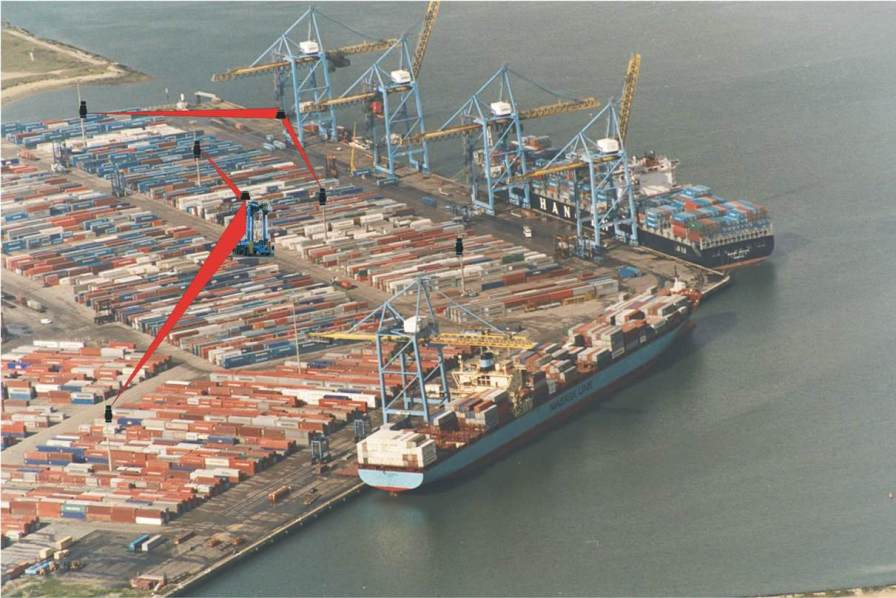
\includegraphics[width=0.6\textwidth]{./chapitres/simulation/bornesLaser.jpg}
  \caption{Réseau de bornes laser implantées sur le Terminal de Normandie (source : \href{http://www.ldtt-fr.com}{http://www.ldtt-fr.com})}
  \label{fig:bornesLaser}
\end{figure}

\begin{figure}[ht]
\centering
 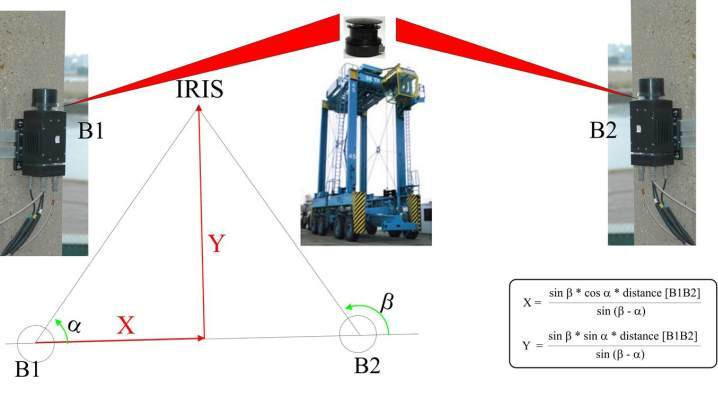
\includegraphics[width=0.6\textwidth]{./chapitres/simulation/triangularisationLaser.jpg}
  \caption{Triangularisation du signal infrarouge entre les bornes IRIS du terminal et celle d'un chariot cavalier (source : \href{http://www.ldtt-fr.com}{http://www.ldtt-fr.com})}
  \label{fig:triangularisation}
\end{figure}

Après plusieurs années de développement et de tests réels, cette technologie se montre performante et fiable et permet de connaître en temps réel la position des engins de manutention au sein du terminal. Cette information est la condition \textit{sine qua non} à toute recherche d'optimisation dynamique des activités des engins de manutention. Grâce à la position des véhicules il est ainsi possible d'optimiser dynamiquement le routage des chariots cavaliers et de prendre en compte les durées de parcours au sein du terminal. Ceci permet par conséquent, d'optimiser l'activité des chariots cavaliers tout en contrôlant le suivi de leurs opérations. En effet, lorsqu'un conteneur est chargé ou déposé par un chariot cavalier, un signal contenant la position du véhicule est envoyé au système. Ainsi, le système connaît la position de prise du conteneur (et par conséquent le conteneur chargé) ainsi que sa position de dépose. Ces informations permettent d'éviter les pertes de conteneurs au sein du terminal.

La partie LITIS du projet consistait à proposer des méthodes d'optimisation dynamique des activités des chariots cavaliers en utilisant l'information fournie par le système de géolocalisation laser. 

	
	%%%%%%%%%%%%%%%%%%%%%%%%%%%%%%%%%%%%%%%%%%%%%%%%%%%%%%%
	%%%%%%%%       Chap 2 : APPLICATION	 	%%%%%%%
	%%%%%%%%%%%%%%%%%%%%%%%%%%%%%%%%%%%%%%%%%%%%%%%%%%%%%%%  
	\chapter{Applications aux terminaux à conteneurs}\label{chapitre:application}

	\section*{Introduction}\label{partie:application-introduction}
	\addcontentsline{toc}{section}{Introduction}
        %Introduction chapitre III : Simulation

Ce chapitre présente $D^2CTS$ : un simulateur de terminal portuaire à conteneurs conçu et développé durant cette thèse. Les problèmes d'ordonnancement et d'affectation ainsi que de routage dynamique sont des problématiques théoriques ici inscrites dans un contexte concret. Les terminaux portuaires à conteneurs sont des structures privées difficilement abordables. Ils fonctionnent en continu et il est donc impossible de procéder à des tests grandeur nature sur une journée d'exploitation. Un simulateur permet ainsi de réaliser ces mesures de performance dans un environnement virtuel le plus réaliste possible avant d'hypothétiquement passer à la mise en place à l'échelle réelle. 

Le programme a été élaboré lors de la participation du LITIS au projet CALAS qui est l'acronyme de \textit{CArrier LAser tracking System}. Le projet consiste à élaborer une technologie de localisation des engins de manutention capable de fonctionner à n'importe quel endroit du terminal. En effet, la technologie de géolocalisation actuelle utilise des satellites (GPS : \textit{Global Positioning System}%TODO CHECK
) afin de déterminer les coordonnées d'un émetteur. Or, le signal des satellites traversant mal le métal, les véhicules qui se trouvent sous les portiques de déchargement ou dans les travées de conteneurs ne sont pas repérés.

La société \textit{Laser Data Technology Terminal} (LDTT) a mis au point une technologie de géolocalisation utilisant un rayon laser et exploitant la caractéristique physique principale des chariots cavaliers : leur hauteur. En effet, les chariots cavaliers sont les engins mobiles autonomes les plus élevés du terminal. Il est donc possible de déterminer leur position grâce à un signal horizontal émis à la hauteur du sommet des chariots cavaliers afin d'être en mesure de localiser les véhicules équipés à n'importe quel endroit du terminal. Le système est composé d'un réseau d'émetteurs/récepteurs laser (\textit{InfraRed Intelligent Sensors}) IRIS répartis sur le terminal (voir figure \ref{fig:bornesLaser}). D'autres bornes IRIS sont installées sur les chariots cavaliers et permettent de réaliser une triangularisation du signal infrarouge (voir figure \ref{fig:triangularisation}).


\begin{figure}[ht]
\centering
 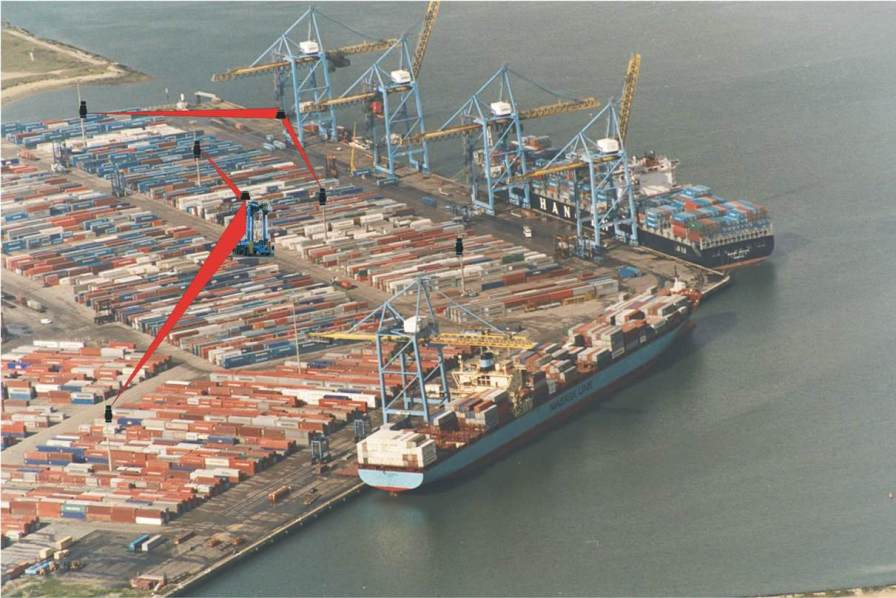
\includegraphics[width=0.6\textwidth]{./chapitres/simulation/bornesLaser.jpg}
  \caption{Réseau de bornes laser implantées sur le Terminal de Normandie (source : \href{http://www.ldtt-fr.com}{http://www.ldtt-fr.com})}
  \label{fig:bornesLaser}
\end{figure}

\begin{figure}[ht]
\centering
 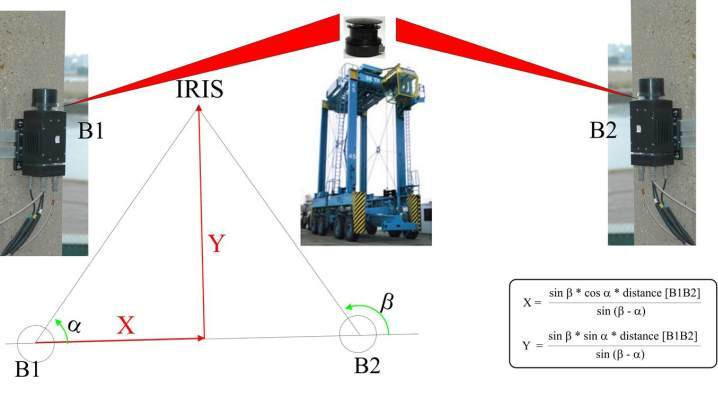
\includegraphics[width=0.6\textwidth]{./chapitres/simulation/triangularisationLaser.jpg}
  \caption{Triangularisation du signal infrarouge entre les bornes IRIS du terminal et celle d'un chariot cavalier (source : \href{http://www.ldtt-fr.com}{http://www.ldtt-fr.com})}
  \label{fig:triangularisation}
\end{figure}

Après plusieurs années de développement et de tests réels, cette technologie se montre performante et fiable et permet de connaître en temps réel la position des engins de manutention au sein du terminal. Cette information est la condition \textit{sine qua non} à toute recherche d'optimisation dynamique des activités des engins de manutention. Grâce à la position des véhicules il est ainsi possible d'optimiser dynamiquement le routage des chariots cavaliers et de prendre en compte les durées de parcours au sein du terminal. Ceci permet par conséquent, d'optimiser l'activité des chariots cavaliers tout en contrôlant le suivi de leurs opérations. En effet, lorsqu'un conteneur est chargé ou déposé par un chariot cavalier, un signal contenant la position du véhicule est envoyé au système. Ainsi, le système connaît la position de prise du conteneur (et par conséquent le conteneur chargé) ainsi que sa position de dépose. Ces informations permettent d'éviter les pertes de conteneurs au sein du terminal.

La partie LITIS du projet consistait à proposer des méthodes d'optimisation dynamique des activités des chariots cavaliers en utilisant l'information fournie par le système de géolocalisation laser. 


	%%%%%%%%%%
	\section{Structure et organisation des terminaux à conteneurs}\label{partie:application-terminaux}
	%Section Structure et organisation des terminaux à conteneurs

\subsection{Structure}
Shématiquement, un terminal portuaire à conteneurs est divisé en 5 parties : 
\begin{itemize}
 \item La zone de stockage (\textit{yard}) : composée de travées de conteneurs empilés sur plusieurs niveaux;
 \item Le dépôt : où les véhicules de manutention sont garés;
 \item La zone des camions : où les camions apportent ou viennent récupérer les conteneurs;
 \item La zone des trains : où les wagons sont acheminés pour être déchargés et/ou chargés;
 \item Les quais : où les porte-conteneurs sont arrimés. 
\end{itemize}

\begin{figure}[ht]
 \label{fig:zonesTN}
 \begin{center}
 \includegraphics[width=0.5\textwidth]{chapitres/application/3zonesDuTN.png}
 \caption{Les 3 principales zones d'échange du Terminal de Normandie}
 \end{center}
\end{figure}

La zone de stockage est divisée en blocs. Chaque bloc comporte une série de travées où sont empilés les conteneurs. La hauteur maximale d'empilement varie en fonction des terminaux. Il y a 3 étages de conteneurs dans la zone de stockage des terminaux du port du Havre.
La zone des trains comporte plusieurs rangées de rails souvent entrecoupées par des routes afin de permettre aux engins de manutention de passer sans devoir faire le tour du train entier.
La zone des camions est constituée à l'entrée du terminal par des guichets où les conducteurs annoncent leur arrivée aux portes du terminal et leur ordre de chargement/livraison. Puis à l'intérieur du terminal des zones camions sont réparties afin d'accueillir les véhicules en attente de (dé)chargement.
La zone des quais comporte des portiques, le plus souvent mobiles permettant de décharger les conteneurs des navires sur les quais ou inversement de charger les conteneurs des quais sur les navires. Il est possible également que des camions se stationnent sous un portique afin de recevoir directement un conteneur du navire déchargé, ou de décharger son conteneur directement dans le navire.

\subsection{Engins de manutention}

Dans \cite{Steenken2004}, Steenken et al. distinguent 2 catégories de véhicules pouvant être rencontrés au sein d'un terminal à conteneurs : d'une part les véhicules des clients (trains, camions et navires) et d'autres part les engins de manutention du terminal.
Le transport des conteneur au sein du terminal peut être soit vertical, soit horizontal. Le transport vertical concerne les opération de levage et de dépose des conteneurs. Les engins concernés sont les portiques de quai ou de stockage. Ces engins sont la plupart du temps mobiles (soit sur rail, soit sur pneus) ce qui permet de les déplacer le long du quai ou le long des travées de stockage (voir fig. \ref{fig:portiqueBarge}. 

\begin{figure}[ht]
 \begin{center}
  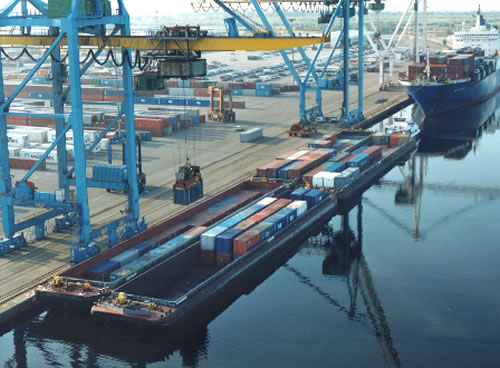
\includegraphics[width=0.5\textwidth]{chapitres/application/portique_barge.jpg}
  \caption{Portique du port du Havre, mobile sur rail, effectuant le déchargement d'une barge (source : \url{http://www.t-n.fr})}
  \label{fig:portiqueBarge}
 \end{center}
\end{figure}

Au contraire, le transport horizontal concerne les véhicules capable de déplacer un conteneur d'un endroit à un autre à l'intérieur du terminal. Les conteneurs doivent ainsi être déplacés entre la zone des camions et le yard, entre la zone des trains et le yard ainsi qu'entre les quais et le yard (et réciproquement du yard vers les zones des camions, trains et navires).
Il existe à l'heure actuelle deux procédés de gestion de ces déplacement : les véhicules passifs et les véhicules actifs.
Les véhicules actifs représente le procédé le plus moderne et consiste à utiliser des véhicules automatiques capables de transporter des conteneurs entre les différentes zones de manutention. Un système de câbles permet de délimiter les couloirs de circulation de ces engins qui sont ensuite capable de s'orienter automatiquement. Ces véhicules sont dis passifs car ils ne sont pas autonomes dans le sens où il ne sont pas capables de charger ou décharger un conteneur par eux-même. Ils doivent attendre d'être chargés ou déchargés par une grue. Ainsi, ces véhicules requirent la présence de portiques dans toutes les zones du terminal. Dans les ports utilisant cette technologie, des portiques sont utilisés pour empiler et dépiler les conteneurs des travées. Les AGV se garent sous le portique afin d'être chargés ou déchargés.

\begin{figure}[ht]
 \label{fig:AGV}
 \begin{center}
 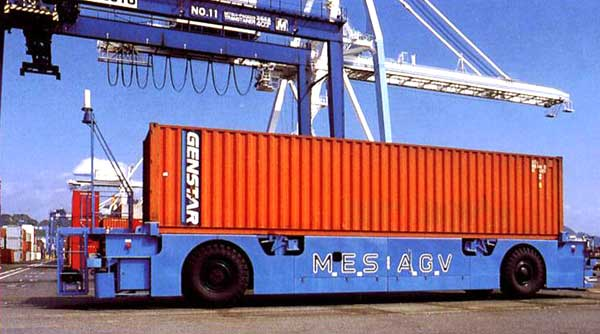
\includegraphics[width=0.5\textwidth]{chapitres/application/agv.png}
 \caption{Automated Guided Vehicle (AGV) de marque MES (source : mescranes.com)}
 \end{center}
\end{figure}

Les véhicules actifs d'autre part, consiste plus traditionnellement à utiliser des véhicules pilotés par des opérateurs et capable à la fois de transporter et de charger ou décharger un conteneur sans l'aide d'un portique. Il existe trois principaux engins de ce type : 
\begin{itemize}
 \item \textit{Forklift Truck} (chariots élévateurs) : ces chariots élévateurs permettent uniquement de manipuler des conteneurs vides. Ils servent donc à déplacer ces conteneurs dans une partie particulière du terminal où ils sont stockés;
 \item \textit{Reach Stacker }(chariots empileurs) : ces chariots sont utilisés pour charger et décharger les trains. La prise se fait par le côté, ce qui reprend l'avantage du chariot élévateur mais en permettant de soulever une charge beaucoup plus lourde;
 \item \textit{Straddle Carrier} (chariots cavaliers) : ces chariots sont les plus puissants. La prise se fait par le dessus. Ils sont capable d'enjamber une pile de conteneurs de 3 étages et permettent ainsi de se déplacer dans les travées.
\end{itemize}

Ce sont ces véhicules qui sont utilisés pour la manutention des conteneurs au sein des terminaux du port du Havre. Certains chariots sont capable d'adapter dynamiquement la longueur de leur pince afin de s'adapter aux différents types de conteneurs. D'autres chariots nécessitent de rentrer au dépôt afin qu'un mécanicien modifie l'écartement des pinces.
\begin{figure}[ht]
 \label{fig:enginsManutention}
 \begin{center}
 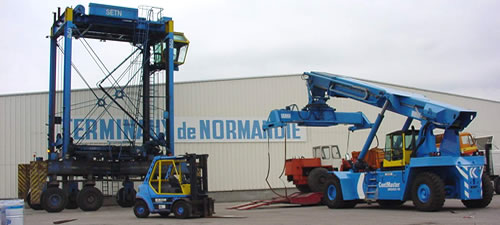
\includegraphics[width=0.5\textwidth]{chapitres/application/enginsTN.png}
 \caption{Engins de manutention utilisés par les Terminaux de Normandie (de gauche à droite) : chariot cavalier, chariot élévateur et chariot empileur (source : \url{http://www.t-n.fr)}}
 \end{center}
\end{figure}

\begin{figure}[ht]
 \label{fig:sc}
 \begin{center}
  \begin{tabular}{ccc}
	  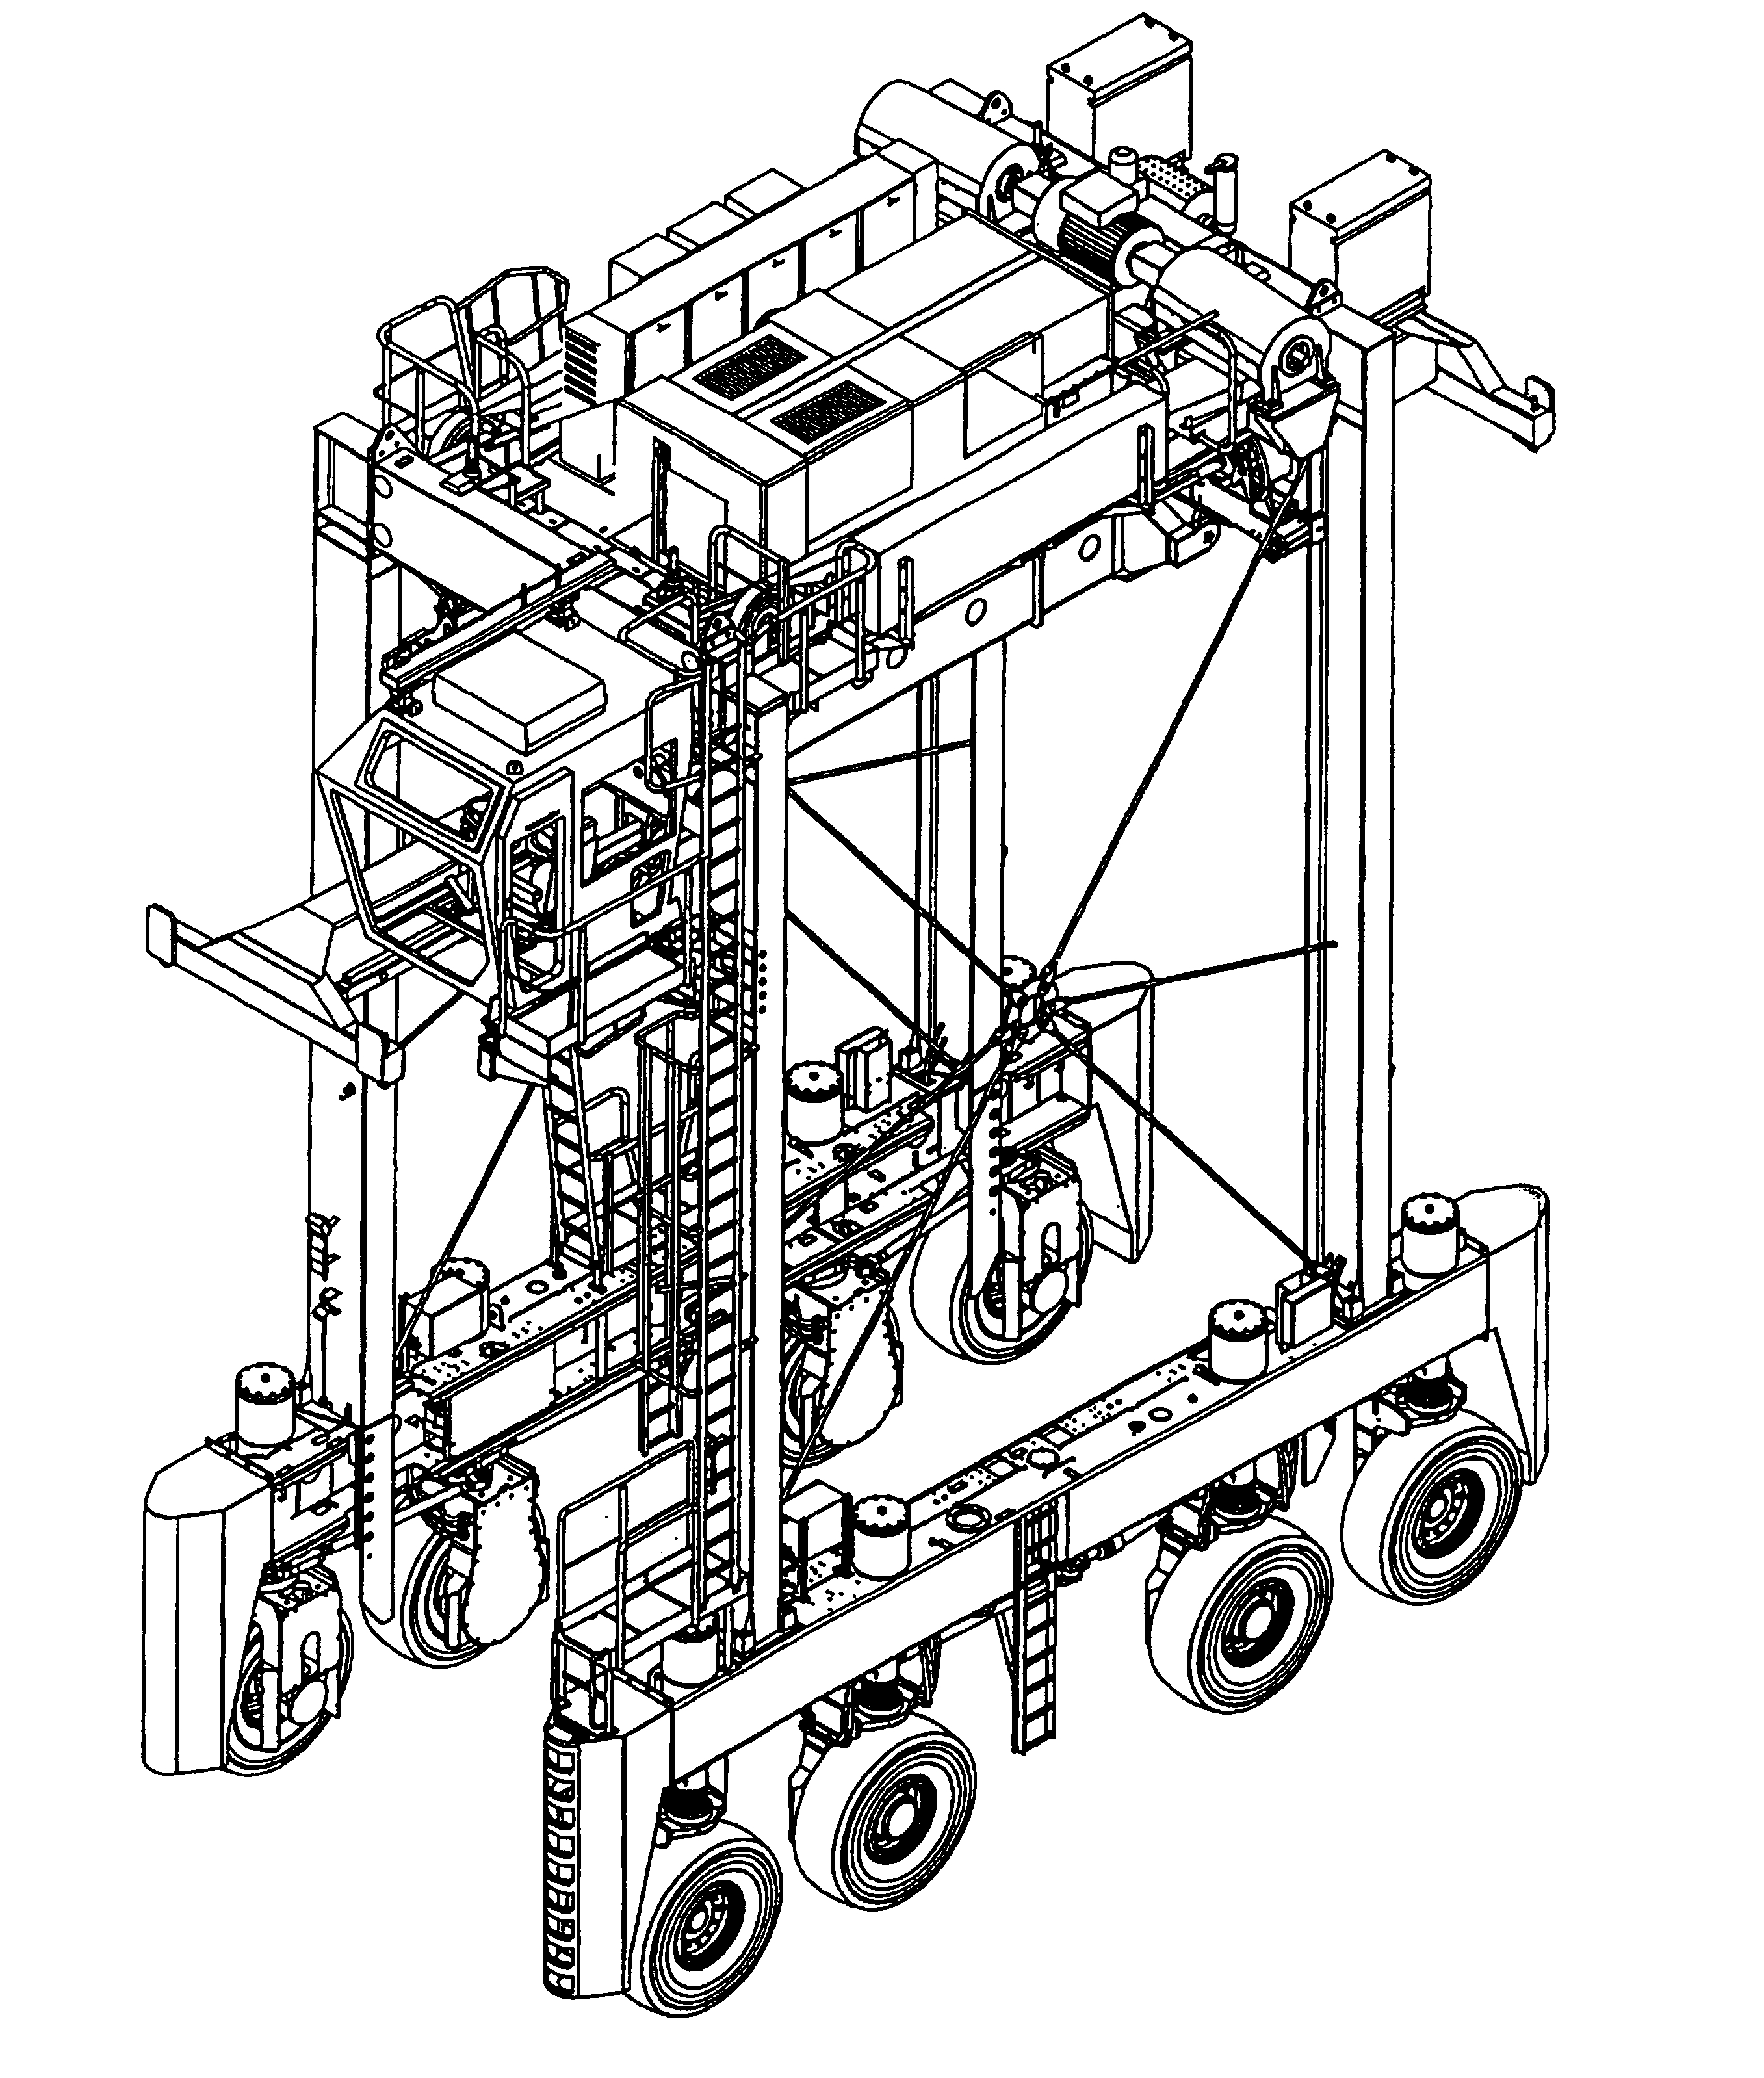
\includegraphics[height=3.5cm]{chapitres/application/schema_sc.jpg} & 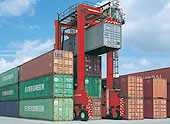
\includegraphics[height=3.5cm]{chapitres/application/tn-straddle-carriers.jpg} & 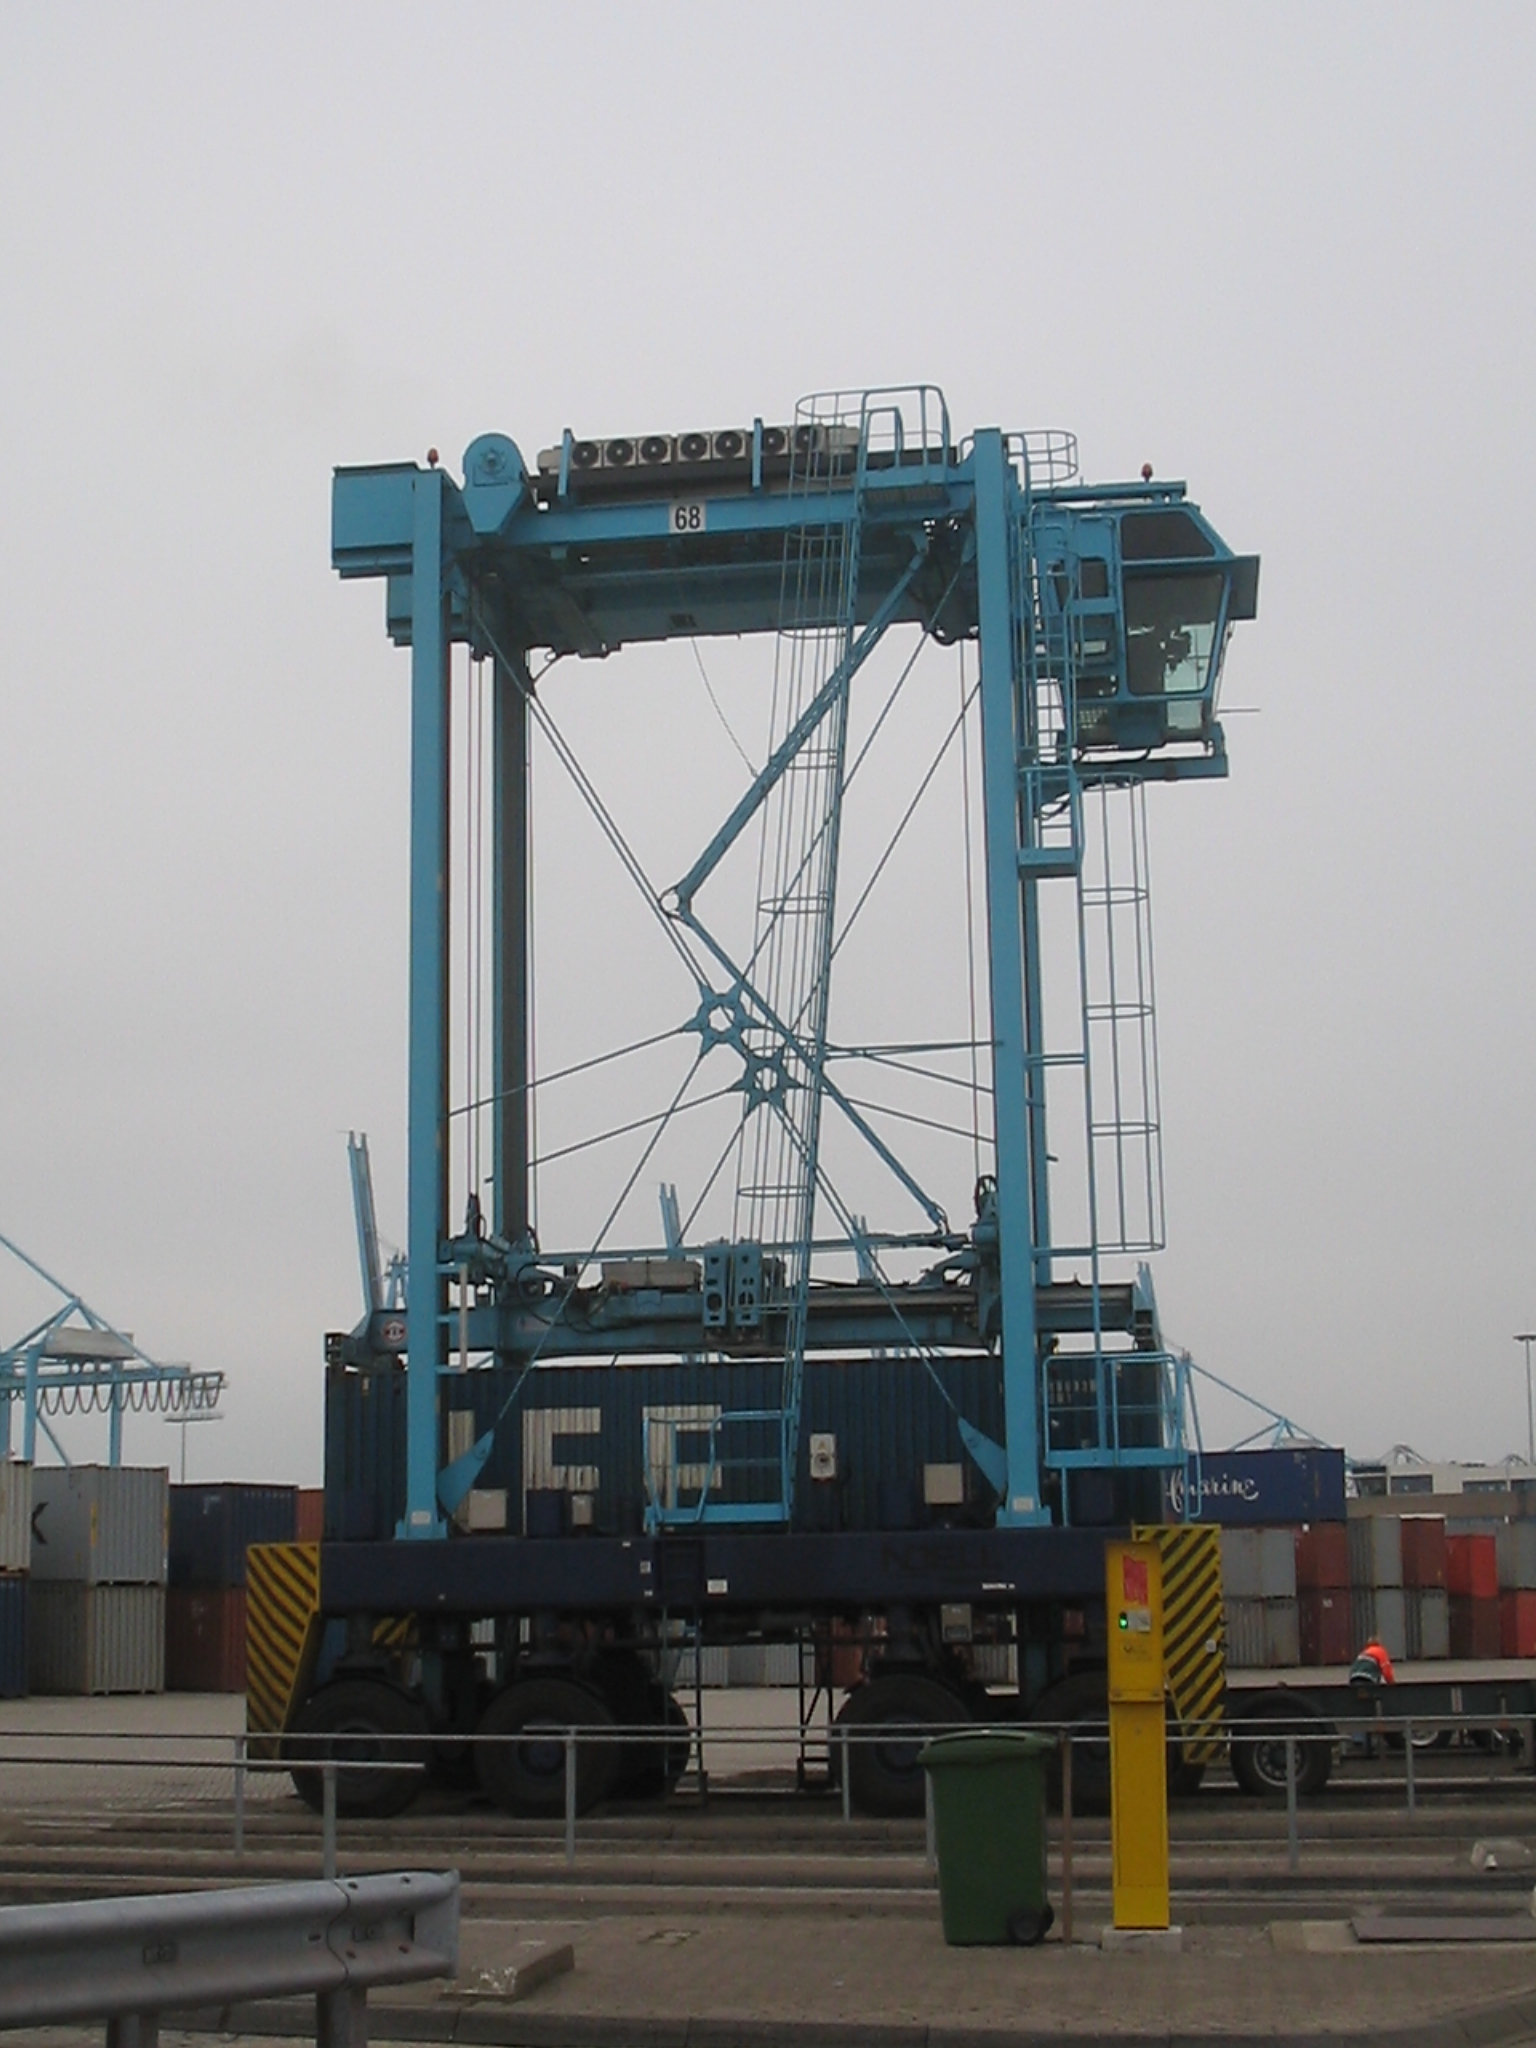
\includegraphics[height=3.5cm]{chapitres/application/containerlift_straddle_carrier.jpg}
  \end{tabular}
 \end{center}
  \caption{Chariots cavaliers}
\end{figure}

Cette thèse prend racine dans le contexte portuaire local et c'est pourquoi il ne sera question que de l'optimisation des déplacement des chariots et non pas des véhicules automatiques. Il est à noter qu'il ne sera fait référence qu'aux chariots cavaliers dans la suite de ce manuscrit tout en gardant à l'idée que les mêmes procédés s'appliquent également aux autres chariots (\textit{forklift trucks} et \textit{reach stackers}).

\subsection{Réseau routier}

Les différents blocs du terminal sont reliés grâce à un réseau constitué de routes et de carrefours. Ce réseau peut être modélisé par un graphe orienté $G=(V,A)$ où $V$ est l'ensemble des carrefours et où $A$ est l'ensemble des routes. Les travées de conteneurs constituent des routes praticables par les chariots cavaliers. Cependant, le fait d'enjamber les conteneurs rend impossible à deux chariots de se croiser ou de se doubler dans une même travée. L'espacement entre deux travée peut de même empêcher deux chariot de se croiser dans deux travées connexes. Ces routes spécifiques peuvent être modélisées par des arcs First-In-First-Out (voir \cite{Orda1990}). Ces arcs garantissent que le premier véhicule utilisant l'arc sera le premier à en ressortir.
Cette spécificité des arcs FIFO a pour conséquence de provoquer des temps d'attente potentiels des chariots en entrée de travée. Ceci peut avoir un impact lourd sur les performances du routage des chariots et doit être pris en compte avec attention. En effet, certaines zones du réseau routier du terminal sont faiblement connexe et peuvent être rapidement saturées. Un routage efficace consistera principalement à ne plus considérer la distance parcourue comme unique critère d'optimisation mais également le temps de parcours.

\subsection{Activités des chariots cavaliers}

Les chariots cavaliers sont utilisés pour déplacer les conteneurs à l'intérieur du terminal. Chaque déplacement est appelé ``mission''. Lorsqu'un chariot n'effectue aucune mission, on dit qu'il est ``libre``. Il stationne alors dans une zone spécifique du terminal appelée ''dépôt``. 
Chaque mission comporte 4 phases. D'abord une phase de déplacement vers le point de collecte, puis la phase de chargement du conteneur sur le chariot, ensuite une nouvelle phase de déplacement mais cette fois vers l'emplacement de livraison, et enfin, la phase de déchargement du conteneur du chariot.

\subsubsection{Les types de missions}
Une mission peut être de 4 types :
\begin{itemize}
 \item Entrée : un conteneur doit être stocké dans le yard
 \item Sortie : un conteneur doit être amené du yard vers une zone d'échange (camion, train ou quai)
 \item Transbordement : un conteneur doit être déplacé d'un quai à un autre
 \item Réorganisation : un conteneur doit être déplacé à l'intérieur du yard
\end{itemize}

La première catégorie de mission concerne le déchargement des camions, trains ou porte-conteneurs. Les chariots se rendent sur l'emplacement de collecte du conteneur (au dessus de la remorque du camion, du wagon, ou sous le portique de quai), prennent le conteneur concerné par la mission, puis se dirigent vers l'emplacement de livraison à l'intérieur du yard et y dépose le conteneur.
La seconde catégorie de mission concerne l'opération inverse, c'est à dire le chargement des camions, trains ou porte-conteneurs. Les chariots se rendent sur l'emplacement de collecte du conteneur dans le yard, prennent le conteneur concerné, puis se dirigent vers l'emplacement de livraison (au dessus de la remorque du camion, du wagon, ou sous le portique de quai) et dépose le conteneur sur le sol dans le cas d'un quai, ou sur la remorque du camion, ou encore sur le wagon du train.
La troisième opération concerne le chargement des conteneurs d'un navire sur un autre porte-conteneurs. Le chariot doit alors récupérer le conteneur de la mission sous le portique de quai, puis se diriger vers le portique de chargement du navire à charger et y déposer le conteneur qui sera acheminé à bord par la grue.
Enfin, l'opération de réorganisation consiste à déplacer les conteneurs à l'intérieur de la zone de stockage afin de préparer l'arrivée (la sortie) de conteneurs du terminal. Cette opération permet d'éviter d'avoir au dernier moment à dépiler un certains nombre de conteneurs pour accéder à un conteneur en bas d'une pile par exemple.

\subsubsection{Fenêtres de temps}

Deux fenêtres de temps sont attribuées à chaque mission. Ces fenêtres indiquent les périodes de temps à respecter d'une part pour collecter le conteneur, et d'autre part pour le livrer.
Si un chariot cavalier arrive avant le début de la fenêtre de temps, il devra attendre. S'il arrive après la fin de la fenêtre de temps, c'est le véhicule client (camion, train, porte-conteneur) qui devra attendre. Cette attente des clients peut provoquer des frais supplémentaires pour le terminal qui devra payer des pénalités de retard. Les fenêtres de temps peuvent être ainsi strictes (\textit{hard}) ou lâches (\textit{soft}). 
Ainsi, les fenêtres impliquant un client seront strictes afin de réduire les coûts, alors que les fenêtres de temps n'impliquant que des véhicules du terminal seront molles. En effet, lors d'une mission de chargement de camion par exemple, la collecte du conteneur à livrer se situe dans le yard. Si le chariot manque sa fenêtre de temps pour la collecte, cela n'entraînera pas de pénalité à payer pour le 
terminal.
La fenêtre de collecte est donc molle. En revanche la livraison du conteneur concerne un camion et le non respect de la fenêtre de temps entraînera des frais de pénalité à payer pour le terminal. La fenêtre de temps de livraison sera donc stricte.

\subsubsection{Objectifs des chariots cavaliers}

%Dire combien un chariot consomme de carburant
%Dire combien coute un chariot cavalier
Un chariot cavalier mesure environ 15 mètres de haut pour 10 mètres de long et 5 mètres de large et pèse près de 60 tonnes à vide.
Capable de déplacer une charge de 50 tonnes à la vitesse de 20 km/h, un chariot peut se déplacer à vide jusqu'à 40 km/h.
Sa consommation de carburant dépasse les 20 L/h. 

\begin{figure}[ht]
  \begin{center}
   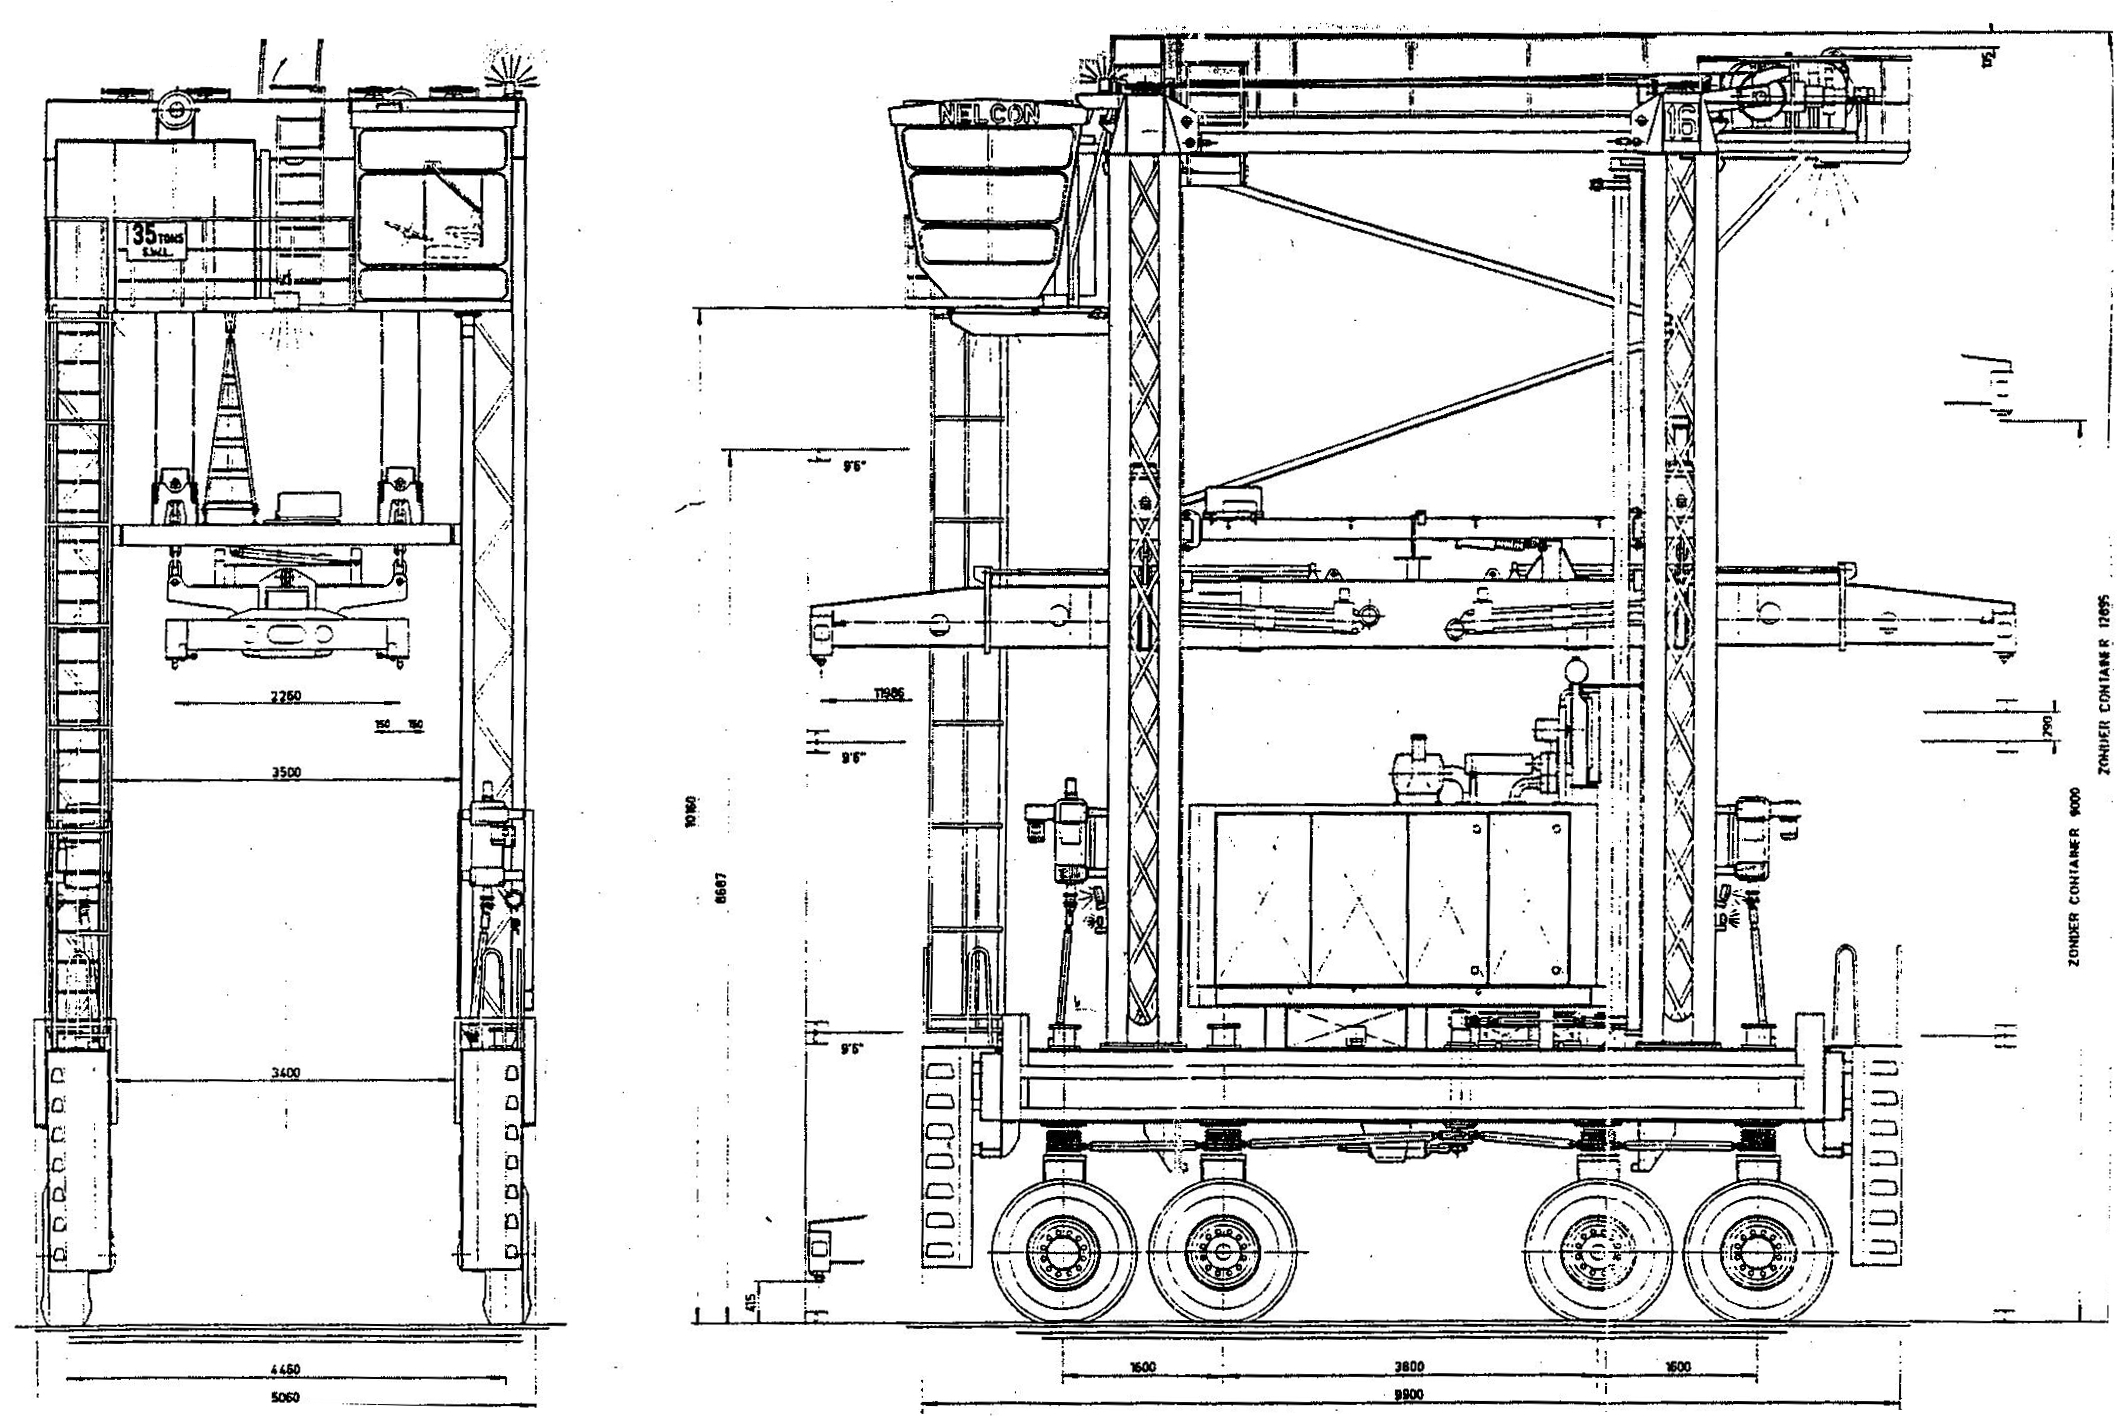
\includegraphics[width=0.9\textwidth]{chapitres/application/planSC.jpg}
   \caption{Plan d'un chariot cavalier utilisé par le port du Havre dans les années 1990}
   \label{fig:application:planSC}
  \end{center}
\end{figure}

Ces caractéristiques techniques font qu'un chariot est extrêmement coûteux à la fois à l'achat (plus de 800000 \geneuro) et à l'utilisation (voir \cite{Huang2003}).
De plus, le pilotage de ces engins requiert une main d'\oe uvre de haute qualité dotée d'une grande précision afin de réaliser des manœuvres complexe impliquant de très lourdes charges en toute sécurité.
Afin de conserver une concentration et une précision accrue, ces pilotes ne peuvent conduire un chariot cavalier que pendant une période donnée dépendant du terminal concerné. Puis une phase de repos doit être respectée avant que le conducteur puisse reprendre son travail. Pour le terminal, cette main d'\oe uvre est un coût conséquent et doit être gérée de façon optimale.

À l`échelle du terminal, l'objectif est comme pour toute entreprise de services de dégager des profits.
Il est donc important de chercher à réduire les coûts et ceci peut être réalisé en partie en minimisant le nombre de chariots à utiliser et cherchant à réduire au minimum les distances parcourues par la flotte de chariots cavaliers.

À l'échelle d'un chariot cavalier, la qualité de service offerte au clients dépendra principalement de deux facteurs. D'une part, le soin pris par le conducteur du chariot pour charger/décharger un conteneur, et surtout d'autre part le respect des fenêtres de temps de la mission. Les caractéristiques temporelles évoquées dans le paragraphe précédent doivent être prisent en compte lors du calcul de l'ordonnancement des missions.

Pour toutes ces raisons et à la fois à l'échelle du terminal et à l'échelle des chariots cavaliers, les objectifs sont double. Pour le terminal, il est nécessaire de minimiser la taille de la flotte d'engins de manutention, de mains d’œuvre... tout en maximisant la qualité de service. À l'échelle des chariots cavaliers, les objectifs sont de minimiser la distance parcourue tout en minimisant le dépassement des fenêtres de temps.

\subsection{Le Terminal de Normandie}

Le Terminal de Normandie est l'un des terminaux du port du Havre. 
Il est situé dans l'estuaire de la seine dans un bassin à marée et est délimité au Nord par deux quais. Le quai d'Asie (au Nord-Ouest) et le quai d'Osaka (au Nord-Est) offrant ainsi à tous les deux 1075 mètres d'accostage et une profondeur de 14 mètres.
La superficie totale du terminal est de 40 Hectares et sa capacité annuelle est de 450000 EVP.

\begin{figure}[ht]
  \begin{center}
    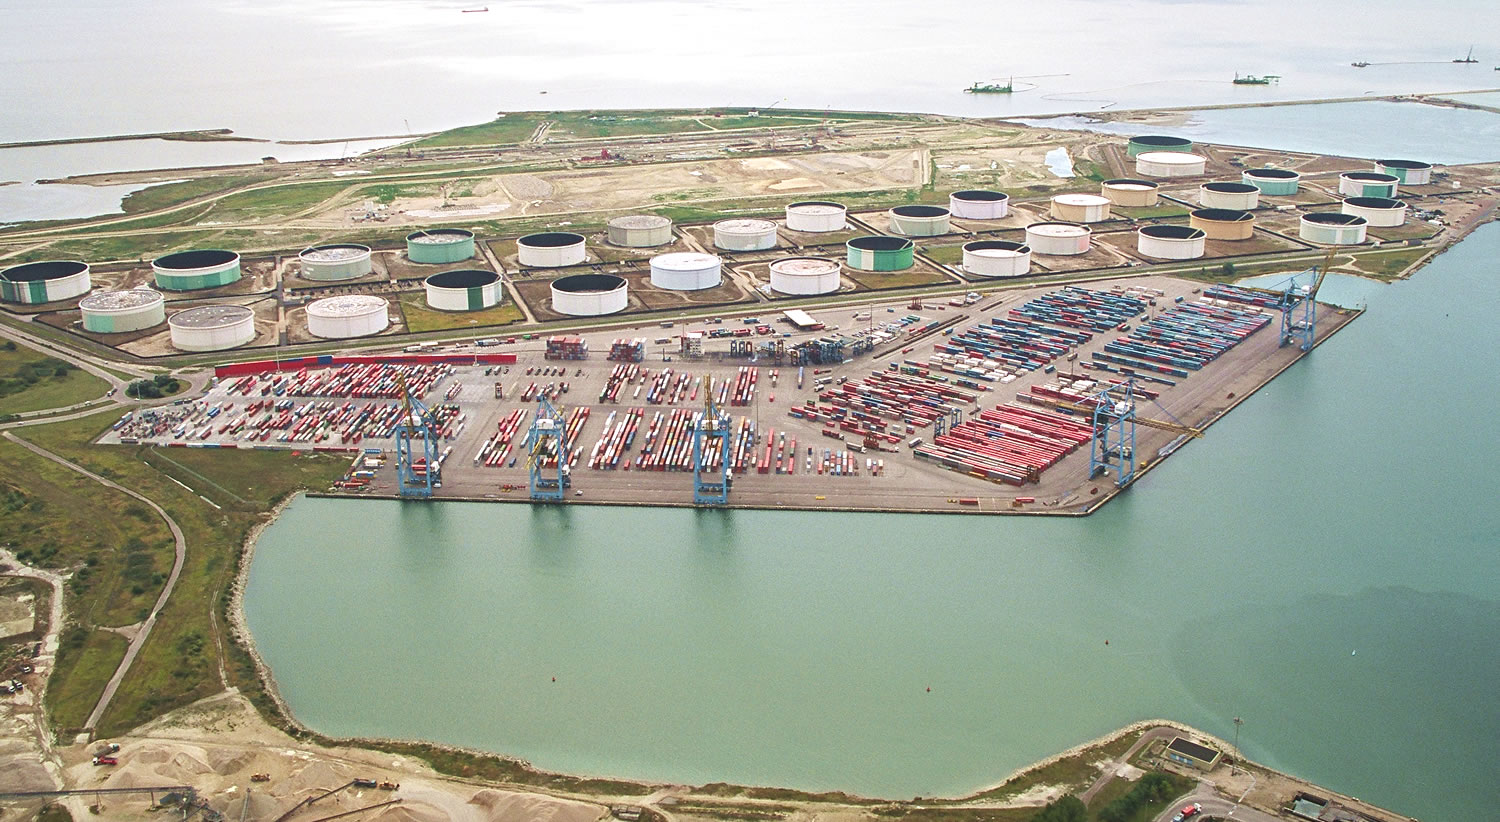
\includegraphics[width=0.8\textwidth]{chapitres/application/terminalDeNormandie.jpg}
    \caption{Terminal de Normandie, Port Autonome du Havre (source : \url{http://www.t-n.fr})}
    \label{fig:TN}
 \end{center}
\end{figure}

Le graphe représentant le réseau routier interne du terminal comporte 1170 sommets, 170 routes et 531 travées pour un total de 3500 emplacements de stockage de conteneurs. La zone de stockage est composée de 12 blocs permettant aisément de disposer les conteneurs à proximité de leur futur zone de transit. La zone des trains comporte 3 voies ferrées différentes entrecoupées sur certaines parties afin de permettre le passage des engins de manutention. Enfin, il existe 3 différentes zones de collecte et de livraison pour les camions.

Ce terminal a été créé en 1990 afin de contenir le flux d'échanges de conteneurs qui n'a cessé d'augmenter de façon de plus en plus importante. À l'époque de sa construction, ce terminal était capable d'accueillir les plus grands navires porte-conteneurs. En revanche, de nouveaux navires géants aux dimensions impressionnantes ont été construits depuis et sont gérés dans un autre terminal du port du Havre construit plus récemment.

\begin{figure}[ht]
  \begin{center}
    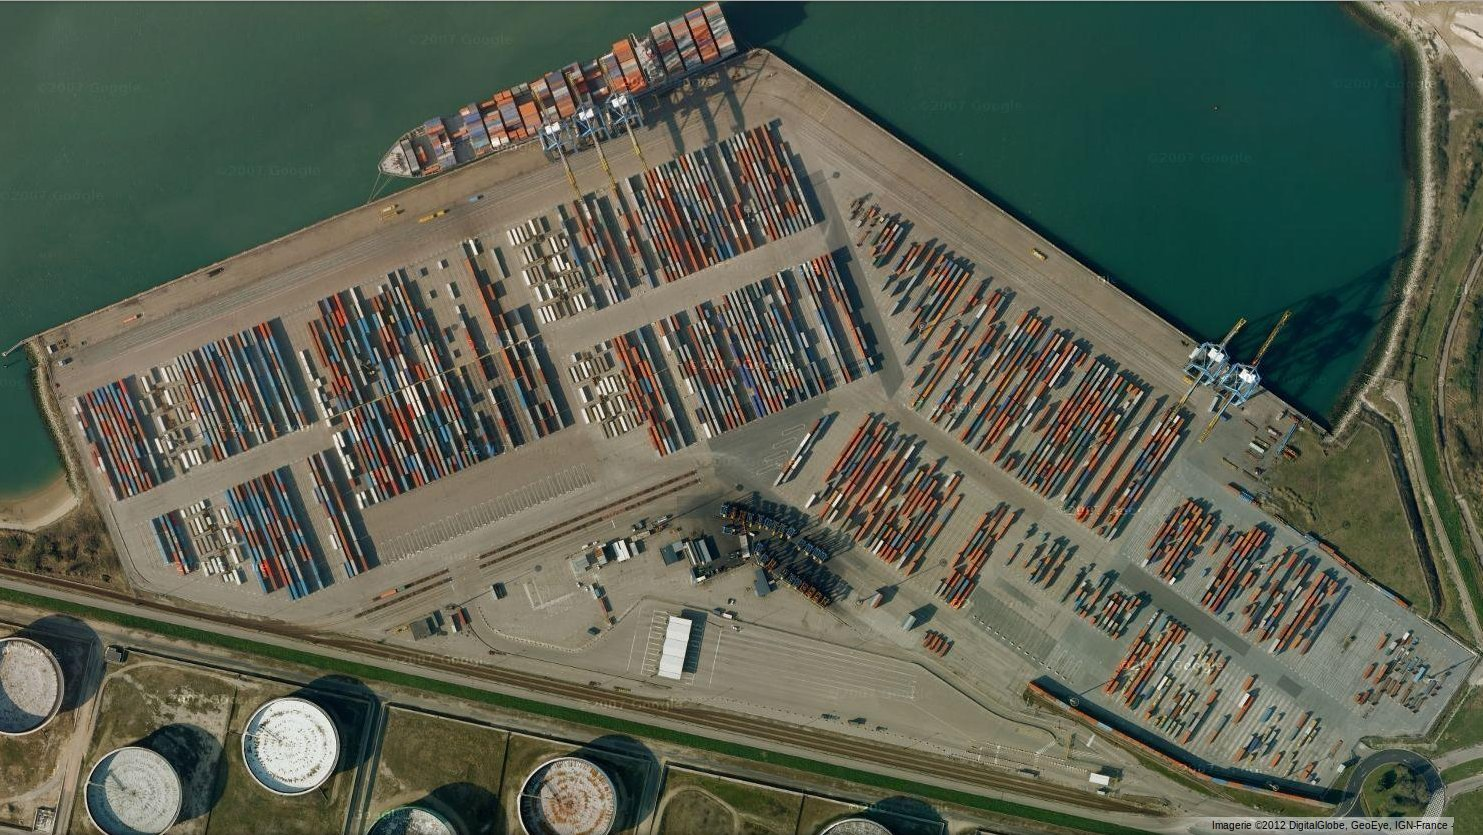
\includegraphics[width=0.8\textwidth]{chapitres/application/terminalDeNormandieGoogleMaps.jpg}
    \caption{Image satellite du Terminal de Normandie, Port Autonome du Havre (source : Google Maps)}
    \label{fig:TNGoogle}
 \end{center}
\end{figure}

5 portiques de quais et une vingtaine de chariots cavaliers assurent la manutention des conteneurs à l'intérieur du terminal où aucun portique n'est utilisé dans la zone de stockage. Les chariots cavaliers sont les seuls engins autorisés à circuler et à manipuler des conteneurs dans les blocs de travées. La régulation du trafic à l'intérieur du terminal est donc un point critique concernant la performance du terminal c'est pourquoi une bonne gestion des engins de manutention est primordiale afin d'assurer une qualité de service suffisante aux clients du terminal.\\


%détailler dans la partie SIMULATEUR la modélisation du terminal ainsi que l'acquisition des données...
	

	%%%%%%%%%%
	\section{Optimisation des terminaux à conteneurs}\label{partie:application-optimisationTerminaux}
	% Section Optimisation des terminaux à conteneurs

\subsection*{Introduction}

Le Terminal de Normandie est un exemple de terminal portuaire à conteneurs parmi tant d'autres. 
De façon générale, un terminal multimodal à conteneurs est une plate-forme logistique où les échanges doivent être réalisés dans le respect de certains critères (emplacements de stockage, fenêtres de temps, ressources humaines, etc.). 
Un certain nombre d'éléments peuvent ainsi être optimisés afin de répondre au mieux aux besoins des clients tout en maximisant les profits pour le terminal.

Les terminaux sont en concurrence les uns avec les autres. Les navires choisissent les ports leur permettant de décharger leur cargaison et de charger de nouveaux conteneurs le plus rapidement possible et pour le coût le plus faible possible. Les ports de Rotterdam, de Hambourg, d'Anvers, de Brême et du Havre sont ainsi en concurrence pour desservir le Nord de l'Europe. 
Il est donc primordial pour ces ports de réduire les coûts d'exploitation tout en assurant une productivité élevée.

On retrouve ainsi de nombreux facteurs d'optimisation dans les terminaux à conteneurs comme : 
\begin{itemize}
  \item la structure du terminal ;
  \item l'allocation des berges aux navires ;
  \item l'allocation des grues de quai ;
  \item les plans de chargement des navires ;
  \item le transbordement ;
  \item la gestion des conteneurs vides ;
  \item la gestion des effectifs ;
  \item le routage des véhicules ;
  \item le stockage (allocation des travées et des blocs) ;
  \item les transferts (quai - stockage, stockage - stockage, stockage - terre) ;
  \item l'allocation des engins de manutention.
\end{itemize}
Ces problèmes sont présents dans la littérature en tant que \textit{Berth Allocation Problem}, \textit{Quay Cranes Scheduling Problem}, \textit{Ship Loading Plan Problem}, \textit{Shortest Path Problem}, \textit{Block and Bay Allocation Problem}, \textit{Vehicle Routing Problem} et \textit{Job Scheduling Problem}. %Add quotes

\subsection{Structure du terminal}

La structure du terminal est un élément déterminant concernant la performance des engins de manutention qui s'y déplacent. Disposer de grandes zones de stockage permet d'obtenir une surface de stockage importante. Toutefois, inévitablement certains blocs se retrouveront plus éloignés d'une ou de plusieurs zones de transfert (quais, rails, zones des camions). Un quai éloigné d'une zone de stockage destinée aux transferts sur les camions engendrera des durées de déplacement plus importants mais permettra par exemple de raccourcir la distance vis-à-vis de la zone de stockage destinée aux trains.

De même, les engins de manutention doivent la plupart du temps retourner au dépôt en cas d'inactivité. La position du dépôt est donc essentielle afin de minimiser la distance à parcourir pour se rendre du dépôt aux points de collecte des conteneurs, puis pour revenir du point de livraison vers le dépôt.

Tout est affaire de compromis entre le positionnement des composantes du terminal ainsi qu'entre le choix de ces éléments et de leur quantité. Les plus grands terminaux disposent de quais immenses mais requièrent également par exemple une distance importante entre l'extrémité d'une berge et une zone de stockage même située au centre du terminal. La plupart de ces terminaux géants sont équipés en conséquence et utilisent des portiques dans les zones de stockage et des engins automatiques pour transporter les conteneurs entre les différentes zones.

Le terminal géant de Yangshan (voir Fig. \ref{fig:optTerminaux:shanghaiCT}), situé à Shanghai en Chine est un exemple de ces paradoxes entre la dimension d'un terminal et sa performance. Il est le plus grand terminal au monde à l'heure actuelle. Même si la construction de ce terminal n'est pas encore terminée, ses quais s'étendent déjà sur 6km de long et comportent 60 portiques. Il a été construit sur une île et a été relié à la métropole chinoise par le \textit{Donghai Bridge}, pont de plus de 35km de long. Le paradoxe de ce terminal gigantesque réside dans 3 points. D'une part il est rentre directement en compétition avec les terminaux déjà existant de Shanghai, ensuite le seul point le reliant au continent est un pont dont le trafic ne pourra être trop important, et enfin, sa capacité est telle qu'il ne sera pas utilisé à plein régime avant plusieurs années. Les coûts d'utilisation d'une telle plate-forme seront donc très élevés ce qui rend le terminal peu attractif vis-à-vis des autres terminaux de la 
ville. L'intérêt majeur du terminal réside dans la profondeur de ses quais qui lui confère la possibilité d'accueillir les plus gros porte-conteneurs actuels. Grâce à cette caractéristique et après étude de la structure du terminal et plus particulièrement de son isolement par rapport à la métropole, le terminal de Yangshan apparaît clairement destiné à des opérations de transbordement.


\begin{figure}[ht]
  \begin{center}
    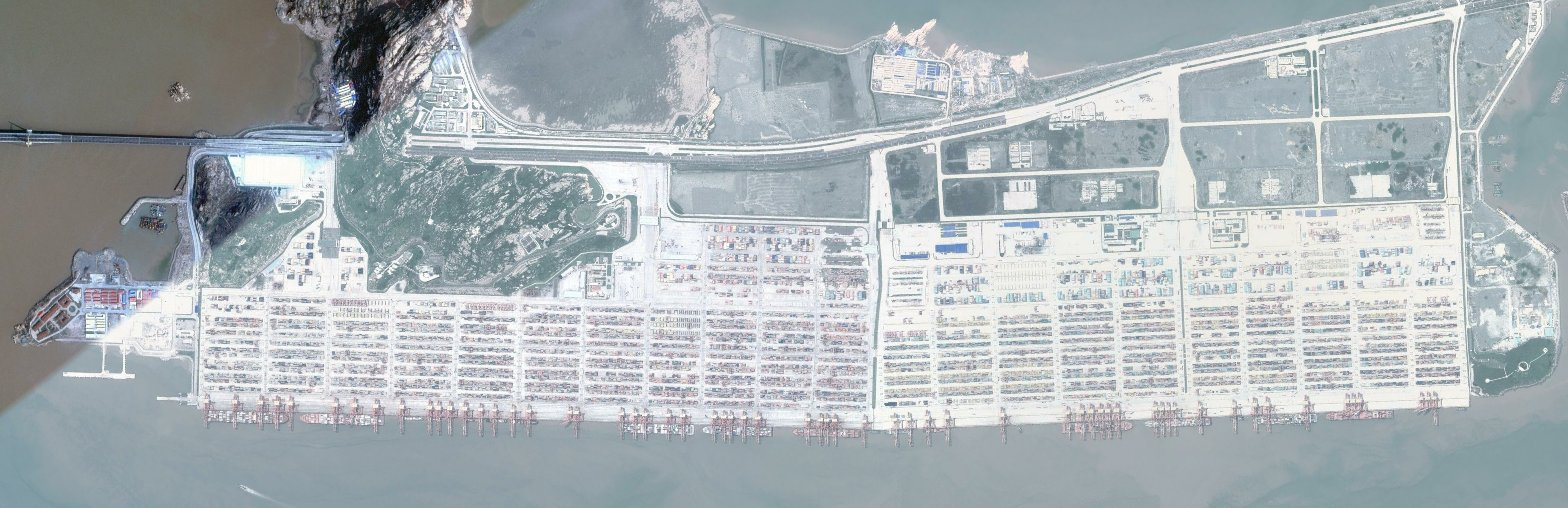
\includegraphics[width=0.8\textwidth]{chapitres/application/terminalDeYangshan.jpg}
    \caption{Terminal de Yangshan à Shanghai en Chine (source : Google Earth)}
    \label{fig:optTerminaux:shanghaiCT}
  \end{center}
\end{figure}

La dimension et l'organisation interne d'un terminal à conteneurs doit donc être étudiée avec le plus grand soin car elle déterminera en grande partie la performance et l'attractivité du terminal.

\subsection{Allocation des berges et transbordement}

Le problème d'affectation des berges (\textit{Berth Allocation Problem} ou \textit{Berth Scheduling Problem}) est l'un des problèmes d'optimisation logistique les plus connus. Il s'agit d'une variante du problème d'affectation quadratique (\textit{Quadratic Assignment Problem}) qui consiste à déterminer l'affectation d'une partie d'un quai à un navire pendant une période donnée de façon à minimiser la durée de service associée au navire (et donc indirectement la distance des déplacements des conteneurs à charger sur le bateau, ou à décharger du bateau, ainsi que les coûts de manutention associés). Tout comme le problème d'affectation quadratique, le problème d'allocation des berges est NP-Difficile.

Ce problème peut se définir dans le cas discret (les quais sont découpés en portions et les navires sont accostés sur un ou plusieurs segments contigus du quai) ou dans le cas continu (le quai n'est pas découpé en parties et les navires peuvent y accoster n'importe où), dans le cas statique (tous les navires sont présents au début du calcul) ou dans le cas dynamique (une partie des navires peuvent être présents au début des calculs, puis les autres arrivent en cours de planification).

Lorsqu'un conteneur doit être déchargé d'un navire pour être chargé sur un autre on parle d'opération de transbordement. Il est alors nécessaire de déterminer conjointement la position d'accostage des deux navires sur le quai afin de minimiser le temps de transfert des conteneurs. 
Lorsqu'un conteneur doit être chargé sur le navire, il faut prendre en compte la distance entre sa position de stockage dans le yard et la position où sera accosté le navire.
Lorsqu'un conteneur doit être déchargé du navire pour être stocké dans le yard, il faut déterminer la position de stockage de ce conteneur en fonction de sa destination future (navire, train ou camion) et chercher un emplacement à la fois proche de la destination et proche du quai où sera accosté le navire. Calculer la position d'accostage du navire revient donc à calculer les emplacements de stockage des conteneurs à décharger de façon à minimiser les déplacements.

%cite

\subsection{Allocation des grues de quai}

Le problème d'affectation des portiques de quai (\textit{Quay Crane Scheduling Problem}) est le problème rencontré une fois le problème de l'affectation du quai résolu, ou du moins en partie résolu. 
En effet, les portiques de quai (\textit{Quay Crane}, \textit{Gantry Crane}, \textit{Container Crane} ou \textit{Ship-to-Shore Crane}) sont des engins de manutention sur rails pouvant mesurer jusqu'à 60 mètres de haut. 
De tels équipements sont extrêmement onéreux et bien souvent les terminaux n'en comportent qu'un nombre restreint. 

Allouer plusieurs portiques au déchargement d'un navire permet de raccourcir la durée de service du navire, mais le portique supplémentaire affecté ne pourra pas être utilisé pour les autre navires accosté au même instant et donc le temps de service des autres navires augmentera.

Les portiques étant posés sur des rails il est impossible de déplacer une grue d'un bout à l'autre du quai si un autre portique se trouve déjà sur le quai. L'affectation d'un portique devra tenir compte de cette caractéristique. 

De même, l'affectation des grues de quai devra également être prise en compte lors de l'affectation de la berge au porte-conteneurs afin de permettre de déterminer son temps de service. 

%cite

\subsection{Positionnement des conteneurs}	%TODO voir avec Monsoria...

Une fois les navires accostés, les portiques affectés au porte-conteneurs se chargent de décharger les conteneurs sur le quai. 
Les conteneurs doivent dans un second temps être acheminés vers un emplacement de stockage en attendant d'être transférés vers un wagon ou un camion ou un autre navire. 
Le choix de cet emplacement doit tenir compte de deux facteurs. D'une part la provenance du conteneur, c'est-à-dire ne pas être situé trop loin du quai dans le cas d'un conteneur déchargé par un portique, ou de la zone du camion ou du train dans le cas d'un conteneur apporté par la route ou par le rail. D'autre part, l'emplacement doit être déterminé en tenant compte de sa destination. Si le conteneur sera chargé sur un wagon alors il devra être stocké dans une travée d'un bloc proche de la zone où le train sera à quai. Si le conteneur sera chargé sur un camion alors d'une part le camion sera dirigé vers une zone d'échange proche du point d'origine du conteneur, et le conteneur sera stocké dans une travée d'un bloc proche de cette zone. Si le conteneur est destiné à être chargé sur un navire, alors il devra être stocké dans la travée d'un bloc à proximité de la portion de quai affectée au navire sur lequel le conteneur devra être chargé.

Il existe également une position verticale à déterminer pour le conteneur. En effet, les conteneurs peuvent être empilés dans les travées sur plusieurs niveaux. Placer un conteneur devant rester dans le terminal longtemps sur le sommet d'une pile alors que les autres conteneurs de cette pile devront être déplacés rapidement engendrera des déplacements supplémentaires. Ces opérations de déplacement consistent un peu comme à la manière du jeu de Hanoï à déplacer temporairement les conteneurs d'une pile sur une autre pile afin de libérer le conteneur posé au sol, puis à reposer les conteneurs supérieurs sur la pile d'origine.
Il est donc important de prendre en compte les fenêtres de temps des missions associées à un conteneur (mission d'entrée du conteneur sur le terminal et mission de sortie du conteneur du terminal) afin de déterminer son emplacement.

Les dates d'entrée et de sortie d'un conteneur sont prises en compte également afin de prioriser l'utilisation d'emplacements proches des zones d'échanges (camions, trains, navires) aux conteneurs transitant peu de temps par le terminal. En revanche, les conteneurs devant rester sur le terminal plus longtemps seront placés plus loin sur les travées de ces zones, ou du moins seront positionnés sur le sol, à la base d'une pile.

Le choix d'un emplacement peut s'avérer difficile si le terminal est saturé. Il peut parfois être nécessaire de déplacer un conteneur à l'intérieur même du yard afin de libérer l'emplacement pour un autre conteneur. Un tel déplacement mobilise un engin de manutention pendant une durée parfois importante et le rend dont inutilisable pour d'autres missions.

Dans le cas statique, où toutes les entrées/sorties de conteneurs sont connues à l'avance, il est possible de déterminer le positionnement optimal des conteneurs afin de minimiser les distances les durées ou de service des clients. En revanche, dans le cas dynamique, les ordres de mission ne sont connues qu'en partie à l'avance, d'autres missions ne seront connues que plus tard, pendant le déroulement de la journée d'exploitation du terminal. Il est dans ce cas impossible de connaître le positionnement optimal des conteneurs de façon exacte. Tout l'enjeu de la résolution de ce problème consiste à déterminer la position optimale des conteneurs à un instant fixé en prennant en compte un facteur de risque lié à la méconnaissance des données.

\subsection{Routage des véhicules} \label{chap:contexte:opt:routageVehicules}

Raccourcir les durées de déplacement entre deux points du terminal permet de réduire le temps de service d'un client. Il est possible d'agir sur 3 facteurs : 
\begin{itemize}
 \item la vitesse de circulation des engins de manutention ;
 \item la limitation de vitesse sur le terminal ; 
 \item le chemin suivi par le véhicule.
\end{itemize}

Le premier facteur dépend des caractéristiques techniques des véhicules, mais touche, comme le second facteur, à la sécurité des personnes et des marchandises sur le terminal. Augmenter la limitation de vitesse d'un engin comme un chariot cavalier demandera aux conducteurs un effort encore plus accru pour maîtriser les 60 tonnes à vide de l'engin et risque de provoquer des accidents aux conséquence lourdes (le conducteur est positionné au sommet de l'engin, soit à plus de 10 mètres du sol).

\begin{figure}[ht]
 \begin{center}
 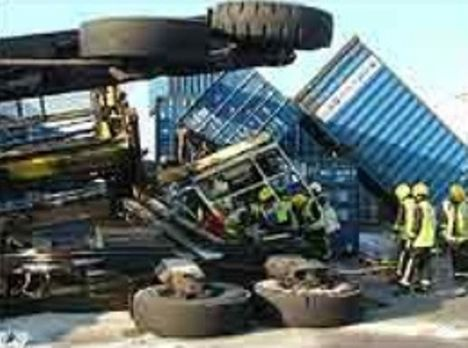
\includegraphics[width=0.4\textwidth]{chapitres/application/sc_crash.jpg}
 \caption{Accident d'un chariot cavalier sur le port d'Essex (Angleterre) le 23 octobre 2007}
 \label{fig:optTerminaux:scCrash}
 \end{center}
\end{figure}

L'unique moyen de chercher à réduire les durées de déplacements au sein du terminal est d'optimiser le guidage des véhicules. 

\subsubsection{Objectifs}
Dans un problème de routage, l'objectif est de minimiser la distance à parcourir entre deux points d'un graphe. 
Comme décrit précédemment, le réseau routier d'un terminal constitue un graphe dont les n\oe{}uds sont les carrefours du terminal et dont les arcs sont les routes et les travées de conteneurs. 

Les chariots cavaliers ont pour objectif d'atteindre des zones de collecte ou de livraisons de conteneurs pendant une fenêtre de temps définie à l'avance. Un routage efficace pour un chariot cavalier consiste donc à atteindre sa destination à l'heure prévue.

Le graphe routier du terminal comporte deux types d'arcs. Si les arcs représentant les routes peuvent facilement absorber un flot de véhicules, les arcs \textit{FIFO} modélisant les travées de conteneurs constituent des points critiques sur le graphe. 
En effet, les chariots cavaliers enjambent les conteneurs empilés dans les travées et ne peuvent donc pas se croiser à l'intérieur de celles-ci. 
Si de tels blocages se produisent ils peuvent causer des retards importants pour la réalisation d'une mission.

Le routage des chariots cavaliers revient à calculer des itinéraires en prenant en compte les temps d'attente en entrée de travées afin de minimiser à la fois la durée totale du parcours (déplacement et attente), le coût de déplacement (consommation de carburant), et l'écart de temps entre la date d'arrivée du chariot et la fenêtre de temps.

\subsubsection{Dynamique du graphe}

Le graphe routier du terminal est donc un graphe partiellement \textit{FIFO} mais ce n'est pas sa seule caractéristique. Ainsi, la durée de parcours d'un arc dépend à la fois de la distance à parcourir (longueur de l'arc) mais également du temps. 

En effet, un chariot cavalier ne se déplace pas à la même vitesse lorsqu'il transporte un conteneur que lorsqu'il se déplace à vide.
Sur le Terminal de Normandie, la vitesse d'un chariot cavalier est de 27km/h à vide contre 23 km/h en charge. 
Il est également à noter qu'un tel véhicule met environ 30 secondes afin d'atteindre les 20 km/h. 
D'autre part la vitesse de circulation d'un chariot cavalier est différente en fonction du type de voie empruntée. 
Ainsi les chariots se déplacent très lentement dans les travées et plus rapidement sur les routes du terminal.

La durée de parcours d'un arc dépend ainsi directement de la vitesse du chariot cavalier, du nombre de décélérations et d'accélérations réalisées, et également du trafic sur l'arc au moment de la traversée.
Les durées d'accélérations et de décélérations se révèlent négligeables en pratique et il est donc possible de simplifier le modèle en ne les prennant pas en compte. La durée de parcours d'un arc $(i,j)$ par un véhicule $v$ au temps $t$ sera représenté par la formule suivante : 

\begin{equation}
 \text{duree(}i,j,v,t\text{)}  = \frac{\text{distance(}i,j\text{)}}{\text{vitesse(}i,j,v,t\text{)}} + \text{attente(}i,j,t\text{)}
 \label{eq:optTerminaux:duree}
\end{equation}

Pour les arcs $(i,j)$ non \textit{FIFO} du graphe, le temps d'attente attente($i,j,t$) sera toujours nul.

\subsubsection{Problème global}

Dans un tel graphe, le problème du plus court chemin en temps peut être résolu en temps polynomial (voir \cite{Orda1990}). 
En revanche, le problème de plus court chemin en coût est NP-difficile (voir \cite{Ahuja2003}). 

Toutefois ce problème devant être résolu pour chaque véhicule du terminal, les résultats du routage d'un véhicule auront un impact sur les caractéristiques du graphe et donc sur le calcul du routage des autres véhicules. 
La résolution globale du problème de routage, c'est-à-dire pour tous les véhicules, repose sur l'ensemble des routages de chaque véhicule (routages locaux). 
Ainsi, lorsqu'un itinéraire est affecté à un chariot cavalier, il est nécessaire de vérifier si une légère modification d'une route déjà établie pour un autre véhicule n'améliorerait pas de façon significative la solution globale. 
Pour trouver la solution globale optimale, il faudrait alors calculer toutes les permutations possibles des solutions locales. 
Ce problème global est donc NP-complet.

\subsection{Ordonnancement et affectation des missions}

L'ordonnancement des missions consiste à déterminer une date d'exécution à chaque mission ainsi qu'à leur affecter une ressource, c'est-à-dire un chariot cavalier. 

%\subsubsection{Deux problèmes dépendants} 

La date d'exécution de la mission dépendra de deux facteurs. D'une part la fenêtre de temps associé à la phase de collecte du conteneur, et d'autre part la position du chariot cavalier affecté à la mission. En effet, la durée du déplacement du véhicule de sa position initiale à l'emplacement de collecte du conteneur sera prise en compte afin de déterminer la date d'exécution de la mission.

D'autre part, le choix du véhicule affecté à la mission dépendra de 2 facteurs. 
Tout d'abord, la compatibilité du véhicule avec la mission. En effet, certains chariots cavaliers ne sont pas capable d'adapter la taille de leur \textit{spreader} sans devoir être modifié au dépôt par un mécanicien. C'est pourquoi, en fonction du type de conteneur à déplacer il sera impossible pour certains véhicules de remplir la mission, ou la date d'exécution de la mission devra prendre en compte la durée de déplacement du chariot vers le dépôt ainsi que la durée de la modification par le mécanicien.
Ensuite, le deuxième facteur de choix du véhicule pour une mission particulière correspond à son activité, c'est-à-dire à son plan de charge au moment de l'ordonnancement. C'est en effet son activité qui déterminera sa position au moment de l'exécution ainsi que sa future destination après avoir accompli la mission planifiée.
L'objectif est de choisir le véhicule dont l'insertion de la mission dans le plan de charge fera le moins augmenter la distance totale parcourue par l'ensemble de la flotte de véhicules, tout en respectant les contraintes temporelles.

Il est clair que le calcul de la date d'exécution de la mission dépend du chariot qui lui a été affecté et que le choix du chariot est fonction de la date d'exécution de la mission. Le calcul des dates d'exécution et l'affectation des missions aux véhicules doivent donc faire partie du même processus de calcul.\\

Ce problème fait l'objet de cette thèse. Nous détaillerons ainsi dans le chapitre suivant, les différentes modélisations du problème ainsi que la méthode de résolution que nous avons élaboré permettant de proposer des solutions de façon dynamique.


	%%%%%%%%%%
	\section*{Conclusions}\label{partie:application-conclusions}
	\addcontentsline{toc}{section}{Conclusions}
	%Conclusion sur l'application

Un terminal multimodal à conteneurs est une plate-forme logistique d'échange de marchandises ouverte à la fois sur la terre et sur l'eau. Leur développement important montre l'importance des enjeux économiques de ces structures qui doivent être de plus en plus performantes en terme de rapidité de service et de coûts d'exploitation.
L'optimisation du terminal est donc essentielle et concerne différents problèmes comme la définition de la structure du terminal, de l'allocation des berges, des portiques de quai, du positionnement des conteneurs, du routage des véhicules ainsi que de l'affectation des opérations de déplacement de conteneurs.\\


Ce chapitre à permis de définir les tenants et les aboutissants du contexte applicatif de cette thèse et à introduit le problème d'ordonnancement et d'affectation des missions aux chariots cavaliers qui sera étudié dans le chapitre suivant.

	%%%%%%%%%%%%%%%%%%%%%%%%%%%%%%%%%%%%%%%%%%%%%%%%%%%%%%%
	%%%%%%%%          Chap 1 : Etat de l'art	%%%%%%%
	%%%%%%%%%%%%%%%%%%%%%%%%%%%%%%%%%%%%%%%%%%%%%%%%%%%%%%%  
	\chapter{Contexte théorique}\label{chapitre:art}
	
	\section*{Introduction}\label{partie:art-introduction}
	\addcontentsline{toc}{section}{Introduction}
	%Introduction chapitre III : Simulation

Ce chapitre présente $D^2CTS$ : un simulateur de terminal portuaire à conteneurs conçu et développé durant cette thèse. Les problèmes d'ordonnancement et d'affectation ainsi que de routage dynamique sont des problématiques théoriques ici inscrites dans un contexte concret. Les terminaux portuaires à conteneurs sont des structures privées difficilement abordables. Ils fonctionnent en continu et il est donc impossible de procéder à des tests grandeur nature sur une journée d'exploitation. Un simulateur permet ainsi de réaliser ces mesures de performance dans un environnement virtuel le plus réaliste possible avant d'hypothétiquement passer à la mise en place à l'échelle réelle. 

Le programme a été élaboré lors de la participation du LITIS au projet CALAS qui est l'acronyme de \textit{CArrier LAser tracking System}. Le projet consiste à élaborer une technologie de localisation des engins de manutention capable de fonctionner à n'importe quel endroit du terminal. En effet, la technologie de géolocalisation actuelle utilise des satellites (GPS : \textit{Global Positioning System}%TODO CHECK
) afin de déterminer les coordonnées d'un émetteur. Or, le signal des satellites traversant mal le métal, les véhicules qui se trouvent sous les portiques de déchargement ou dans les travées de conteneurs ne sont pas repérés.

La société \textit{Laser Data Technology Terminal} (LDTT) a mis au point une technologie de géolocalisation utilisant un rayon laser et exploitant la caractéristique physique principale des chariots cavaliers : leur hauteur. En effet, les chariots cavaliers sont les engins mobiles autonomes les plus élevés du terminal. Il est donc possible de déterminer leur position grâce à un signal horizontal émis à la hauteur du sommet des chariots cavaliers afin d'être en mesure de localiser les véhicules équipés à n'importe quel endroit du terminal. Le système est composé d'un réseau d'émetteurs/récepteurs laser (\textit{InfraRed Intelligent Sensors}) IRIS répartis sur le terminal (voir figure \ref{fig:bornesLaser}). D'autres bornes IRIS sont installées sur les chariots cavaliers et permettent de réaliser une triangularisation du signal infrarouge (voir figure \ref{fig:triangularisation}).


\begin{figure}[ht]
\centering
 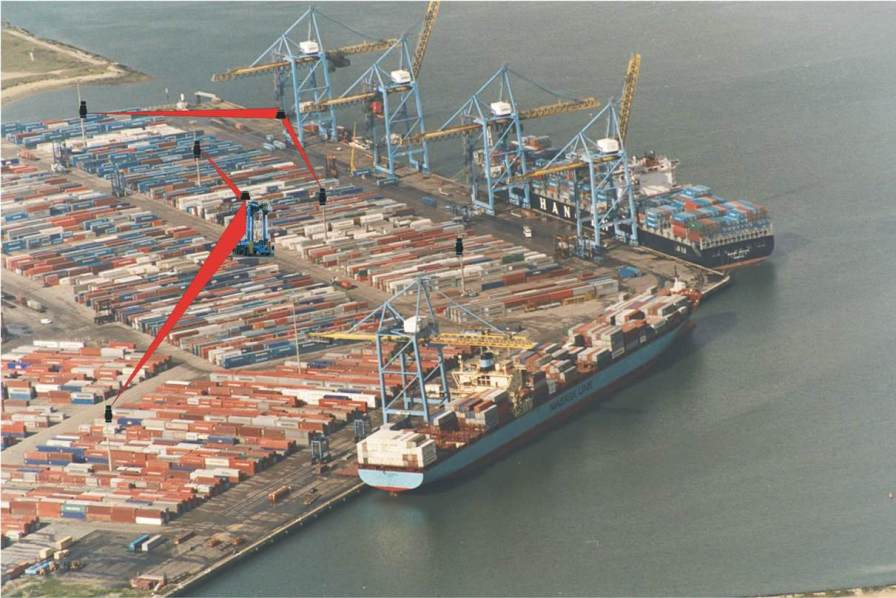
\includegraphics[width=0.6\textwidth]{./chapitres/simulation/bornesLaser.jpg}
  \caption{Réseau de bornes laser implantées sur le Terminal de Normandie (source : \href{http://www.ldtt-fr.com}{http://www.ldtt-fr.com})}
  \label{fig:bornesLaser}
\end{figure}

\begin{figure}[ht]
\centering
 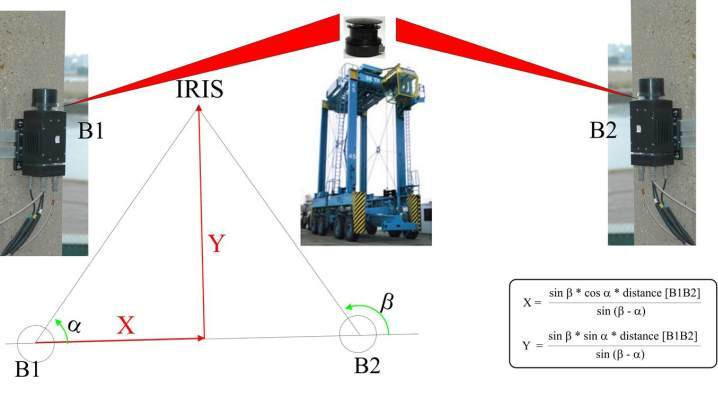
\includegraphics[width=0.6\textwidth]{./chapitres/simulation/triangularisationLaser.jpg}
  \caption{Triangularisation du signal infrarouge entre les bornes IRIS du terminal et celle d'un chariot cavalier (source : \href{http://www.ldtt-fr.com}{http://www.ldtt-fr.com})}
  \label{fig:triangularisation}
\end{figure}

Après plusieurs années de développement et de tests réels, cette technologie se montre performante et fiable et permet de connaître en temps réel la position des engins de manutention au sein du terminal. Cette information est la condition \textit{sine qua non} à toute recherche d'optimisation dynamique des activités des engins de manutention. Grâce à la position des véhicules il est ainsi possible d'optimiser dynamiquement le routage des chariots cavaliers et de prendre en compte les durées de parcours au sein du terminal. Ceci permet par conséquent, d'optimiser l'activité des chariots cavaliers tout en contrôlant le suivi de leurs opérations. En effet, lorsqu'un conteneur est chargé ou déposé par un chariot cavalier, un signal contenant la position du véhicule est envoyé au système. Ainsi, le système connaît la position de prise du conteneur (et par conséquent le conteneur chargé) ainsi que sa position de dépose. Ces informations permettent d'éviter les pertes de conteneurs au sein du terminal.

La partie LITIS du projet consistait à proposer des méthodes d'optimisation dynamique des activités des chariots cavaliers en utilisant l'information fournie par le système de géolocalisation laser. 

	
	%%%%%%%%%%
	\section{Dynamique et incertitude en optimisation}\label{partie:art-Incertitude}
	\label{sec:incertitude}


\subsection{Définition}
%Définition d'optimisation
L'optimisation peut être définie comme le processus visant à améliorer une situation vis-à-vis de son niveau de performance actuel. Mathématiquement, l'optimisation revient à minimiser ou maximiser une fonction objectif en agissant sur des paramètres tout en respectant un ensemble de contraintes. Par exemple, un commerçant cherche à définir le prix de vente de chacun de ses produits afin de maximiser son bénéfice global. Le but ici est de chercher le prix permettant de générer le plus de ventes. Un prix trop élevé repoussera les clients alors qu'un prix trop faible ne permettra pas de dégager suffisamment de marge. Stratégiquement, il est possible de définir un prix très faible pour un ensemble de produits afin d'attirer les clients dans la boutique et ainsi de pouvoir fixer un prix plus élevé sur les autres produits. Mathématiquement cet exemple consiste à maximiser la fonction $\sum \limits_{i=1}^n \left( (P_i-p_i)\cdot q_i \right)$, où $P_i$ est le prix d'achat de l'article $i$, $p_i$ son prix de vente et 
$q_i$ la quantité vendue.

On distingue deux types d'optimisation. Tout d'abord l'optimisation déterministe dans laquelle la réaction du système à la modification des paramètres est parfaitement calculable. D'autre part l'optimisation sous incertitude dans laquelle des composantes du système sont inconnues ou mal connues et peuvent rendre inadaptée voire inapplicable la solution calculée.

%Opt sous incertitude
L'incertitude peut être décrite de façon stochastique ou bornée. Dans le premier cas, on cherche généralement à optimiser le système dans le cas moyen (minimiser l'espérance mathématique de la fonction d'évaluation). Dans la représentation par intervalle borné, c'est le pire des cas qui est la plupart du temps l'objet de l'optimisation. Ainsi, une plage de valeurs possibles est prise dans un intervalle donné, et le cas le plus défavorable est utilisé afin de garantir un niveau de performance peu importe la dégradation du système liée à l'incertitude. On parle ainsi d'optimisation robuste. Le critère du regret maximal est également très répandu en optimisation robuste. Il se définit comme l'écart minimum entre les valeurs obtenues sur différents scénarios pour chaque stratégie étudiée.  %citer des papiers sur l'opt robuste
%figure pour le regret ?

%Opt Dynamique
Parallèlement, on distingue l'optimisation statique de l'optimisation dynamique. Dans cette dernière, le système évolue dans le temps. Dans ce cas, il devient nécessaire d'adapter les paramètres au cours de cette évolution, on parle alors de contrôle optimal (ou commande optimale). Chaque action aura des conséquences sur l'état futur du système. Dans le cas d'un problème déterministe il sera possible de calculer l'évolution du système en fonction de chaque action (scénarios, trajectoires). En revanche, si de l'incertitude est introduite dans le système, il devient impossible de prévoir son comportement futur. Par exemple, un système de guidage missile qui tente de calculer la trajectoire permettant d'atteindre un objectif en dépensant le moins d'énergie possible, adaptera la trajectoire si l'objectif est mobile. Le déplacement de l'objectif peut-être totalement prévisible (train, autre missile...) ou incertain (véhicule piloté par un humain). Dans ce dernier cas, il faudra effectuer des corrections de 
trajectoire à chaque nouvel état du système.

% Dans sa thèse de doctorat (voir \cite{Chachuat2001}), Chachuat a défini l'optimisation comme ``la démarche qui consiste à améliorer une performance, par rapport à un état de référence, sous l'action d'un ou plusieurs paramètres''. L'auteur donne également une définition de l'optimisation statique et dynamique : ``lorsque le comportement du procédé est décrit par des relations algébriques entre les variables d'état et les paramètres du système, on parle d'optimisation statique. Lorsqu'au contraire le procédé présente une évolution temporelle, i.e. lorsque l'évolution dynamique du système est décrite par des relations d'état différentielles, on parle d'optimisation dynamique''.

%Optimisation transformation en problème décisionnel
\subsection{Optimisation et problème décisionnel}
Tout problème d'optimisation peut être vu comme un problème décisionnel. En effet le problème peut être énoncé de la façon suivante : existe-t-il une valeur de $V$ pour laquelle $f(V) \leq k$ ? Avec $V$ vecteur de paramètres et $k$ une valeur donnée. Par exemple, le problème bien connu du sac-à-dos (\textit{Knapsack Problem}) consiste à choisir des objets ayant chacun un poids $p_i$ et une valeur $v_i$, pour remplir un sac-à-dos en cherchant a maximiser la somme des valeurs sans dépasser le poids maximal autorisé $p_{MAX}$. Le problème peut être formulé de la façon suivante. Pour chaque $x_i$, variable binaire indiquant si l'objet $i$ est mis dans le sac ($x_i=1$) ou non ($x_i=0$), existe-t-il une valeur pour laquelle $\sum \limits_{i=1}^{n} p_ix_i \leq p_{MAX}$ et $\sum \limits_{i=1}^{n} v_ix_i \geq v$ pour $v$ donné ? Il suffit pour résoudre ce problème de procéder de façon itérative en diminuant la valeur de $v$ et d'arrêter la recherche dès qu'aucune solution n'est trouvée pour un $v$ donné.

%NP-complétude
Notons qu'un problème de décision peut-être NP-complet alors qu'un problème d'optimisation ne peut-être que NP-difficile. Ainsi, sous forme de problème d'optimisation, le problème du sac-à-dos est NP-difficile, alors que dans sa version décisionnelle, ce problème est NP-complet.\\

%Prise de décision et incertitude
La plupart des problèmes d'optimisation proviennent de situations réelles dans lesquelles des décideurs doivent agir en prenant en compte leur environnement afin de prendre la décision qui s'adapte le mieux à la situation rencontrée. Mais dans certains cas, voire dans la plupart des cas réels, les décideurs n'ont qu'une connaissance partielle de leur environnement, parfois même une vision subjective, biaisée par leur vécu et leurs émotions. Comment est-il  possible, dans ces conditions, de déterminer les actions à réaliser pour obtenir la meilleure réponse possible au problème d'optimisation ?

\subsection{Identifier l'incertitude}

L'incertitude peut provenir de 3 sources différentes :
\begin{itemize}
  \item le jeu de données
  \item le scénario
  \item l'interprétation
\end{itemize}
La première source concerne l'incertitude sur les données du problème. Dans un problème d'ordonnancement par exemple, il peut s'agir d'incertitude au niveau des durées d'exécution des tâches, ou de la date limite. Il peut également s'agir des coûts de traitement, des probabilités de panne du système, etc.

L'incertitude liée au scénario concerne le contexte de l'application de la solution calculée. Ainsi, le coût de la main d’œuvre, le prix du carburant ou de l'électricité pour les machines, par exemple, font partie du contexte de l'exécution.

Enfin, l'incertitude liée à la subjectivité du décideur influence également la qualité de la solution calculée. Les valeurs ainsi que la culture propre à chaque individu influencent son comportement et provoque des divergences dans ses réactions. Par exemple, une personne habituée à jouer au casino sera plus enclin à prendre des risques qu'un gestionnaire habitué à rationaliser chaque décision. Toute décision prise en fonction d'éléments subjectifs est une source d'incertitude.\\

Après avoir identifié les sources potentielles d'incertitude dans un problème, il est nécessaire de déterminer la façon dont elle va être gérée.
%Faut-il gérer l'incertitude ?
\subsection{Gérer l'incertitude}
 
Il existe des moyens de gérer l'incertitude. Les systèmes prenant en compte cette incertitude sont dits pro-actifs, ou anticipatifs. Ils ont pour objectif de calculer une solution robuste, c'est-à-dire valable peu importe les valeurs prises par les éléments sujets à l'incertitude.

Toutefois cette gestion est limitée aux cas où l'incertitude est quantifiable (obéit à une loi stochastique par exemple) ou bornée. Lorsque l'incertitude est trop importante, c'est-à-dire que les éléments sujets à l'incertitude sont trop nombreux ou que l'incertitude n'est pas quantifiable, il est impossible d'envisager une prise en compte efficace. Il est important dans ce cas d'être réactif fasse à la découverte de nouvelles informations concernant le problème. Les systèmes comportant cette spécificité sont appelés systèmes réactifs. Dans ces systèmes, il est possible de détecter une variation si l'application d'une solution calculée ne donne pas les même résultats escomptés. Il est alors possible d'agir afin de prendre en compte cette variation dans le calcul d'une nouvelle solution. 

Dans cette thèse nous ne voulons pas essayer de prévoir l'imprévisible, de faire des prédictions, mais plutôt, à contrario, de s'adapter à tout événement. C'est pourquoi la solution proposée dans la suite de ce manuscrit sera inscrite dans la classe des systèmes réactifs. De plus, nous nous baserons sur la robustesse non pas de la solution proposée, mais plutôt par la robustesse de l'algorithme permettant d'obtenir la solution.


%Optimisation Dynamique
\subsection{Gestion de la dynamique} \label{subsec:dynamique}
%Def
L'optimisation dynamique peut être définie comme le processus visant à améliorer une situation vis-à-vis de son niveau de performance actuel au fil du temps. La fonction mathématique à minimiser ou maximiser sera également dépendante du temps. Dans \cite{Powell1995}, Powell et al. ont défini : 
\begin{itemize}
 \item qu'un problème est dynamique si au moins l'un de ses paramètres est fonction du temps;
 \item qu'un modèle est dynamique s'il incorpore de façon explicite les interactions entre les activités au fil du temps;
 \item qu'une application est dynamique si le problème sous-jacent doit être résolu à chaque fois qu'une nouvelle information est reçue.\\
\end{itemize}


%Dynamique : évolution du systeme
Du fait de l'évolution temporelle du système, une solution calculée au temps $t$ peut ainsi devenir caduque au temps $t+n$. À l'inverse de l'optimisation statique, il n'existe aucune garantie sur la stabilité des composantes du système dans le temps. Par exemple, le commerçant qui cherche à définir ses prix de vente pour maximiser son bénéfice devra prendre en compte l'évolution des prix d'achat de ses marchandises ainsi que le pouvoir d'achat de sa clientèle. La solution calculée à l'ouverture de son commerce ne sera peut-être plus la solution optimale six mois plus tard. Dans cet exemple, le commerçant a besoin d'informations concernant ses ventes afin de pouvoir calculer ses prix (quantité vendue). Il est donc possible de s'appuyer sur les résultats précédents pour définir les prix futurs. En revanche, dans le cas où l'optimisation est basée sur la situation courante, à l'instant $t$, il est impossible d'utiliser la solution calculée précédemment. La dynamique joue alors un rôle hautement perturbateur 
dans le processus d'optimisation et le plus souvent rend impossible l'application de méthodes de résolution exacte qui demanderont un temps de calcul supérieur à la durée de validité de la solution fournie.\\


%Dynamique et incertitude
En optimisation, la dynamique peut être vue comme un vecteur d'incertitude. Les composantes du système apparaissent, disparaissent, et évoluent au fil du temps. La connaissance que l'on a du système, sa perception, est alors elle même sujet à la dynamique. La dynamique étant une source d'incertitude elle peut provenir du jeu de données (les valeurs des données changent au fil du temps), du scénario (des événements surviennent au cours de l'exécution), ou de l'interprétation (la perception du décideur peut évoluer).\\

Dans \cite{Psaraftis1988,Psaraftis1995}, Psaraftis a identifié les problèmes liés à la dynamique dans le cadre d'un problème de tournée de véhicules (\ref{sec:vrp}) :
\begin{itemize}
 \item \textbf{évolution} : prise en compte du temps;
 \item \textbf{qualité} : l'information est de meilleur qualité lorsqu'elle est connue en avance;
 \item \textbf{incertitude} : l'état futur du système est incertain;
 \item \textbf{importance des événements proches du terme} : plus un événement est proche de sa date de déclenchement, plus il est important pour le système;
 \item \textbf{importance du mécanisme de mise à jour de l'information} : il faut être en mesure de communiquer efficacement les multiples variations d'information dans le système;
 \item \textbf{réajustements} : les solutions calculées au préalables peuvent devenir sous-optimales avec le temps;
 \item \textbf{réduction des temps de calcul} : besoin de pouvoir recalculer une solution entre deux événements;
 \item \textbf{report infini} : possibilité de devoir retarder une tâche à l'infini si des nouvelles tâches plus urgentes arrivent au fil du temps;
 \item \textbf{fonction objective adaptée à la dynamique} : les fonctions objectif classique peuvent ne plus s'appliquer au problème car bien souvent l'horizon de planification est inconnu;
 \item \textbf{flexibilité des contraintes temporelles} : il est parfois plus avantageux, dans les problèmes dynamique, de dépasser une fenêtre de temps plutôt que de décaler une tâche dont la fenêtre de temps n'est pas atteinte;
 \item \textbf{optimisation des ressources} : le fait de ne pas connaître l'évolution de la demande fait qu'il est difficile de réduire au minimum le nombre de ressources à utiliser (engorgement), d'autre part une partie des ressources risquent de ne pas être utilisées si la demande est insuffisante.
\end{itemize}
 

%Mesure de dynamicité
On parle de dynamicité d'un scénario lorsqu'on mesure la part de dynamique dans le problème. Dans \cite{Larsen2000}, Allan Larsen indique trois principales mesures du degré de dynamicité.

Tout d’abord, le degré de dynamicité (\textit{Degree Of Dynamism} : \textbf{dod}) est défini par Lund et al. (voir \cite{Lund1996}) comme le rapport entre le nombre de requêtes dynamiques et le nombre total de requêtes (voir eq. \ref{eq:dyn:dod}). Une requête est dite statique si elle est connue avant le début de la planification. Une requête est dite dynamique (on trouve également le terme ``immédiate'' dans la littérature) si elle n'est connue qu'une fois que l'exécution a commencé.
\begin{figure*}[h]
 \begin{equation}
    \label{eq:dyn:dod}
    dod = \frac{\eta_d}{\eta_s+\eta_d}
 \end{equation}
\end{figure*} 

Si cette mesure permet de quantifier la part de dynamique dans un scénario, elle ne permet pas d'évaluer son influence sur le système. En effet, cette mesure ne prend pas en compte la date d’arrivée des requêtes. Si les requêtes dynamiques entrent dans le système en début de scénario, le système est considéré comme aussi dynamique que si elles entraient en toute fin. Pourtant, plus ces requêtes sont connues tard et plus le système doit être réactif afin de calculer une solution dans les temps. Ces retards ont donc un impact négatif sur les performances et il est important de les prendre en compte dans la mesure de dynamicité. Pour cette raison, Larsen a défini le degré effectif de dynamicité (\textit{Effective Degree Of Dynamism} : \textbf{edod}) selon l'équation \ref{eq:dyn:edod}.
Ici, $\eta_s$ et $\eta_d$ sont respectivement le nombre de requêtes statiques et dynamiques. $t_i$ est la date d’arrivée d’une requête $i$ (avec $0 < ti < T$ ) et $T$ correspond à la date de fin de scénario. Cette
mesure prend en compte la moyenne des dates d’arrivées des requêtes dans le système. Plus les requêtes dynamiques arrivent tard, et plus $edod$ sera important. Si $edod = 0$, alors le système est totalement statique. Si $edod = 1$, le système est purement dynamique.
%formule
\begin{figure*}[h]
 \begin{equation}
    \label{eq:dyn:edod}
    edod = \frac{\sum \limits_{i=1}^{\eta_d}\left( \frac{t_i}{T} \right)}{\eta_s+\eta_d}
 \end{equation}
\end{figure*}

Un certain nombre de problèmes d'optimisation utilisent des fenêtres de temps comme pour le problème de voyageur de commerce (voir \ref{sec:tsp}), le problème de tournées de véhicules (voir \ref{sec:vrp}) ou encore les problèmes d'ateliers (voir \ref{sec:jssp}). Larsen a adapté $edod$ afin de prendre en compte l'écart temporel entre la date d'arrivée d'une requête dans le système et sa date d'exécution au plus tard. En effet, si une requête est connue à la fin de sa fenêtre de temps, le respect de celle-ci est problématique. En revanche, une requête arrivant bien avant sa date limite pourra être traitée dans les temps. Le degré effectif de dynamicité avec fenêtre de temps (\textit{Effective Degree Of Dynamism with Time Window} : \textbf{edod-tw}) se défini selon l'équation \ref{eq:dyn:edod-tw} où $r_i$ est le temps de réaction (\textit{reaction time}) de la requête $i$, ce qui correspond à l'écart entre la date d'exécution au plus tard de la requête $i$ et sa date d'arrivée dans le système ($t_i$).
\begin{figure*}[h]
 \begin{equation}
    \label{eq:dyn:edod-tw}
    edod-tw = \frac{1}{\eta_s+\eta_d} \cdot \sum \limits_{i=1}^{\eta_s+\eta_d} \left( 1 - \frac{r_i}{T} \right)
 \end{equation}
\end{figure*} 

Ces mesures permettent de quantifier de façon efficace la difficulté introduite dans le système par la dynamique.

\subsection{Méthodes de résolutions adaptées aux environnements dynamiques}

Les modifications provoquées par la dynamique imposent une grande réactivité de la méthode de résolution du problème. Pour pouvoir prendre en compte les solutions calculées pour un instant $t$, dans le calcul de solutions valides à $t+n$, il faut que la méthode d'optimisation utilise une forme de mémoire. C'est pour cette raison que les méthodes de recherche tabou, les réseaux de neurones artificiels, les algorithmes génétiques ainsi que les algorithmes fourmis sembles adaptés et seront détaillés dans les paragraphes suivants.

\subsubsection{Recherche tabou}
La recherche tabou (Tabu Search), a été proposée pour la première fois par Glover en 1986 (voir \cite{Glover1986}\cite{Glover1989}\cite{Glover1990}). Elle consiste à voyager dans l'espace des solutions  à partir du voisinage de la solution courante en ne conservant que la position minimisant la fonction objectif. Afin d'empêcher l'algorithme de visiter une nouvelle fois des parties de l'espace de recherche déjà étudiées, une sorte de mémoire est ajoutée sous forme de liste tabou dans laquelle les solutions déjà épuisées sont insérées. Appliquée au problème du voyageur de commerce, cette méthode consiste à construire un tour grâce à une heuristique quelconque (plus proches voisins par exemple) puis d'étudier les solutions voisines en inversant deux à deux les positions des arêtes à l'intérieur du tour. La meilleure solution ainsi obtenue est alors étudiée à son tour et la solution de départ est ajoutée à la liste tabou. L'algorithme se poursuit tant que le nombre maximal d'itérations n'est pas atteint ou que 
toutes les solutions voisines sont déjà dans la liste tabou.

\subsubsection{Réseaux de neurones artificiels}
Les réseaux de neurones artificiels (Artificial Neural Networks) ont été introduits par McCulloh et Pitts en 1943 (\cite{McCulloch1943}). Ils se sont basés sur les observations de W. James, père du concept de la mémoire associative qui a défini un principe de fonctionnement qui deviendra plus tard la loi de Hebb. Ainsi, en 1949, Hebb a expliqué le conditionnement chez l'animal (expérience du chien de Pavlov par exemple), par les propriétés des neurones. Selon lui, il est donc possible de modifier les réactions d'un animal vis-à-vis d'un stimulus grâce à un processus d'apprentissage. En 1948, Von Neumann défini l'automate cellulaire (voir \cite{Neumann1966}). Cet automate est capable d'accomplir une tâche élémentaire et de se multiplier pour y parvenir. Les automates cellulaires sont à la base notamment du jeu de la vie de Conway (voir \cite{Conway1970}), où l'état des cellules est déterminé en fonction de règles de voisinage.\\

%Neurone artificiel et réseaux de neurones : définition
Un neurone artificiel est un automate pourvu d'une fonction de transfert (non linéaire bornée). Cette fonction a pour entrée un vecteur $x$ associé à un vecteur $w$ de pondération (coefficients synaptiques) ainsi qu'à un éventuel biais ($b$) (voir fig. \ref{fig:tsp:nn:potentiel}). La fonction d'activation peut-être continue ou à seuil (voir fig. \ref{fig:tsp:nn:fonctionSeuil}), et s'active ou non en fonction du signal reçu en entrée.\\

\begin{figure}[h]
  \centering
  $y=f(\sum \limits^{N}_{i=1} w_i\cdot x_i + b)$
  \caption{Potentiel d'activation d'un neurone}
  \label{fig:tsp:nn:potentiel}
\end{figure}

\begin{figure}[h]
  \begin{equation*}
  f(x)= \begin{cases}
        1 & \text{si } x>0\\
        -1 & \text{sinon}
       \end{cases}
  \end{equation*}
  \caption{Exemple de fonction d'activation à seuil}
  \label{fig:tsp:nn:fonctionSeuil}
\end{figure}

Dans un réseau de neurones, les neurones sont reliés les uns aux autres par des relations de voisinage formant ainsi un graphe orienté. L'activation ou la non-activation des neurones prédécesseurs d'un neurone déterminera la sortie de ce neurone.\\

Les réseaux de neurones peuvent être bouclés ou non. Dans un réseau non bouclé, le graphe représentant le réseau est acyclique. Dans les réseaux bouclés (ou récurrents), le graphe contient au moins un cycle.\\

La pondération des neurones peut être déterminée par un processus d'apprentissage qui peut être supervisé ou non. L'apprentissage supervisé consiste à fournir des paramètres d'entrée associés à des valeurs de sorties désirées. Les poids sont donc modifiés afin d'assurer l'obtention de la sortie fournie. Dans le cas de l'apprentissage non supervisé, aucune sortie désirée n'est fournie et il s'agit alors de déterminer les poids permettant de grouper les composantes de $X$ selon une fonction $F_w$ permettant une bonne généralisation (voir \cite{Kohonen1982}).\\

%Réseaux de Neurones en optimisation
Concernant le domaine de l'optimisation, le premier champ d'application fut la reconnaissance de formes. Ainsi, en 1957, Rosenblatt a développé le modèle du Perceptron (voir \cite{Rosenblatt1958}). En 1960, Widrow a introduit le modèle Adaline (\textit{Adaptative Linear Element}, voir \cite{Widrow1960}) basé sur le perceptron de Rosenblatt mais utilisant un processus d'apprentissage différent, qui sera plus tard à l'origine de l'algorithme de rétropropagation de gradient utilisé couramment avec les Perceptrons multicouches.

%Les limites
En 1969, Minsky et Papert ont montré dans \cite{Minsky1969} les limites du modèle du Perceptron, ce qui a eu pour effet de décourager la recherche sur les réseaux de neurones artificiels.

%A new hope...
Suite à l'article de Hopfield (voir \cite{Hopfield1982}), en 1982, utilisant une méthode d'apprentissage basée sur un résultat escompté, les recherches sur les réseaux de neurones artificiels reprennent. Ainsi, en 1983, la Machine de Boltzmann permet de lever les limitations du Perceptron décrites par Minsky. En 1985, apparaît l'algorithme d'apprentissage par rétropropagation de gradient, utilisé dans les réseaux multicouches.

%Cartes auto-adaptatives
Plus récemment, des réseaux de neurones appelés cartes auto-organisatrices (ou auto-adaptatives) ont été développé par Kohonen (voir \cite{Kohonen1982}). Elles peuvent être utilisées notamment pour la compression de données, d'images. Le principe est d'entraîner un réseau de neurones afin de reproduire une image d'entrée sans recopier chacun de ses pixels. Dans le cas d'une image en couleurs, chaque pixel peut être codé grâce à 3 entiers $r$, $v$ et $b$ tels que $0\leq r, v, b < 2^8$, décrivant une couleur par ses composantes : rouge ($r$), vert ($v$) et bleu ($b$). Un pixel peut donc être stocké sur 24 bits (3 octets). Une image de résolution $1980$x$1080$ comporte $2073600$ pixels, et représente donc $49766400$ bits (environ 5.93Mo). Le but de la compression est de diminuer le nombre de pixels à stocker sans pour autant dégrader l'image de façon trop importante. Pour cela chaque neurone sera chargé de décrire un groupe de pixels de l'image. Les neurones sont initialisés de façon aléatoire, puis un 
processus d'apprentissage non-supervisé permet de déterminer quels 
neurones décrivent le mieux chaque groupe de pixels. Le résultat de la compression regroupe la description de chaque neurone ainsi que les couples $\{$groupe de pixels, neurone descripteur$\}$.\\

\subsubsection{Algorithmes génétiques}

Les algorithmes génétiques (Genetic Algorithms) sont une métaheuristique reposant sur la théorie de l'évolution. Cette méthode générale a été introduite en 1954 par Barricelli (voir \cite{Barricelli1957}) puis développée par Fraser à partir de 1957 (voir \cite{Fraser1957}). Mais c'est à partir des travaux de Holland dans les années 1970 (voir \cite{Holland1975}) que les algorithmes génétiques se sont démocratisés.
%Fonctionnement
Le principe est de représenter une solution (ici appelée individu) sous forme de chromosome (suite de gènes). Un nombre important d'individus (population, ou génome) est généré. Puis des opérateurs génétiques sont appliqués sur les gènes des chromosomes~:
\begin{itemize}
 \item \textbf{La sélection}~: cet opérateur consiste à déterminer quels individus seront conservés dans la génération suivante
 \item \textbf{Le croisement}~: cet opérateur consiste à simuler la reproduction de deux individus et ainsi à créer un nouvel individu conservant une partie des gènes de chacun de ses parents (hérédité).
 \item \textbf{La mutation}~: cet opérateur vise à altérer une partie des gènes d'un individu. Le but est de favoriser l'exploration de l'espace de recherche afin d'empêcher de piéger l'algorithme sur des optima locaux.
\end{itemize}

L'algorithme se déroule de la façon suivante. Tout d'abord une population initiale est générée (la plupart du temps de façon aléatoire). Les individus sont évalués. L'opérateur de sélection est ensuite appliqué et permet de sélectionner des couples d'individus. La génération suivante ne comportant pas les individus non sélectionnés, la population est complétée par les résultats de l'opérateur de croisement sur les individus sélectionnés. Enfin, l'opérateur de mutation est appliqué sur une très petite partie des individus (choisis de aléatoirement) et consiste généralement à ne modifier qu'une infime portion de leur génome afin de ne pas annihiler les effets de la sélection et du croisement sur la convergence de l'algorithme. Le processus est répété un nombre fixé d'itération ou quant la meilleure solution trouvée atteint un score objectif préalablement fixé.

La plus grande difficulté dans l'implémentation de cet algorithme réside dans le codage des chromosomes. En effet, il faut que les chromosomes puissent être facilement construits tout en permettant d'appliquer les opérateurs sans provoquer d'inconsistance. Ainsi, dans certains problèmes il est impossible de croiser deux individu sans garantir la validité de l'individu ainsi créé. Or, c'est bien cet opérateur de croisement qui permet d'améliorer la convergence de l'algorithme et lui permet d'être plus performant qu'une recherche basée sur un recuit simulé ou une recherche tabou. D'autre part, la fonction d'évaluation d'un individu doit être rapide à calculer car c'est d'elle (ainsi que de la taille du problème) que dépendra le temps d'exécution de l'algorithme.
%Détailler les méthodes de sélection ?
Il existe bien-sûr différentes méthodes de sélection des individus. Les plus courantes sont~: 
\begin{itemize}
 \item la sélection par rang~: les n meilleurs individus sont choisis
 \item la sélection par tournoi~: deux individus aléatoirement choisis sont mis en compétition, celui ayant le meilleur score est sélectionné
 \item la sélection uniforme~: les individus ont tous la même probabilité d'être choisis
 \item la sélection par probabilité~: les individus ont une probabilité $p_i = \frac{score_i}{\sum_n^{N}{score_n}}$ d'être choisis.
\end{itemize}

\subsubsection{Algorithmes fourmis}
L'optimisation par colonie de fourmis (Ant Colony Optimization) est également une métaheuristique basée sur une observation du vivant.

Cette technique est issue de l'observation de Deneubourg en 1983 (voir \cite{Deneubourg1983}) et 1989 (voir \cite{Goss1989}) qui a montré que les fourmis étaient capable collectivement de trouver le plus court chemin entre leur nid et une source de nourriture.
En effet, Deneubourg a observé que les fourmis commençaient à coloniser les chemins de façon aléatoire puis au fil du temps commençaient à suivre le même chemin. Il s'avère que ce chemin est le plus court.
Ce phénomène est dû à la méthode de communication des fourmis. Elles utilisent un marqueur chimique~: la phéromone afin d'indiquer, dans le cas d'une recherche de nourriture, l'attractivité d'un chemin.
Ainsi, un chemin permettant de trouver de la nourriture contiendra de la phéromone et sera donc suivi par les autres fourmis de la colonie.

Le point fort de cette méthode de communication indirecte, appelée stigmergie (voir \cite{Grasse1959}), est de permettre de trouver un chemin optimal sans pour autant qu'il n'ai été parcouru en totalité par une fourmi. En effet, la solution optimale est construite en cherchant le chemin comportant le plus de phéromone entre le nid et la source de nourriture. Les fourmis construisant leurs chemins en déposant de la phéromone, c'est bien la somme des dépôts de toutes les fourmis qui permettra de découvrir le chemin globalement optimal. Chaque individu agit positivement sur le choix des composantes du chemin (processus auto-catalytique).

D'autre part, la phéromone étant volatile, le chemin comportant le plus de phéromone sera celui sur lequel elle se sera le moins évaporée.
Ce sera donc le chemin le plus court qui contiendra le plus de phéromone.
Ce phénomène d'évaporation (rétroaction négative) permet également aux fourmis de ne pas réutiliser des chemins qui étaient les plus attractifs (les plus court) au moment de leur découverte.

L'algorithme de colonie de fourmis fut inventé par Dorigo lors de sa thèse en 1991 (voir \cite{Dorigo1992} et \cite{Dorigo1991}). Il a indiqué que la méta-heuristique pouvait s'appliquer à tout problème d'optimisation~: recherche de plus court chemin, problèmes d'ordonnancement de tâches, problème de tournées de véhicules, problème d'affectations quadratique, etc.
Les fourmis artificielles de Dorigo et al. sont légèrement différentes des fourmis réelles. Elles ont une mémoire leur permettant d'éviter de coloniser des morceaux de chemin qu'elles ont déjà parcouru. D'autre part, leur vision leur permet de choisir une destination en fonction de la distance vis à vis de leur position courante. Ce sont ces légères différences qui vont permettre aux algorithmes fourmis de converger plus rapidement vers la solution optimale.

Dans \cite{Dorigo1992}, Dorigo et al. présentent l'algorithme $Ant$-$System$ avec 3 variantes concernant le marquage des chemins~: $Ant$-$density$, $Ant$-$quantity$ et $Ant$-$cycle$.

$Ant$-$System$ est défini comme suit~: 
\begin{itemize}
  \item Soit $\tau_{ij}(t)$ l'intensité de la trace de phéromone sur l'arc $(i,j)$ au temps $t$ ;
  \item Soit $\Delta_{ij}(t,t+1)$ la quantité de phéromone déposée sur l'arc $(i,j)$ par les fourmis entre le temps $t$ et $t+1$ ;
  \item Soit $\rho$ un coefficient de persistance de la trace de phéromone tel que $0\leq\rho\leq1$ ;
  \item À chaque fin de parcours les traces de phéromones sont ainsi mises à jour (eq. \ref{eq:as:evoph})~: 
  \begin{equation}
    \tau_{ij}(t+1)=\rho\cdot\tau_{ij}(t)+\Delta_{ij}(t,t+1)
    \label{eq:as:evoph}
  \end{equation}
  \item Soit $\eta_{ij}$ l'attractivité de l'arc $(i,j)$ (représentant l'inverse de sa longueur ($1/d_{ij}$ dans le cas d'une recherche de plus court chemin par exemple).
  \item Une fourmi $k$ choisi sa destination en fonction de la loi de transition proportionnelle suivante (eq. \ref{eq:as:transition})~: 
  \begin{equation}
   p_{ij}(t) =
   \begin{cases}
    \frac{[\tau_{ij}(t)]^\alpha\cdot[\eta_{ij}]^\beta}{\sum\limits_{l \in \text{visibles}} [\tau_{il}(t)]^\alpha\cdot[\eta_{il}]^\beta} & \text{si } j \text{ n'a pas déjà été visité}\\
    0 & \text{sinon}
   \end{cases}
   \label{eq:as:transition}
  \end{equation}
  où $\alpha$ et $\beta$ sont des paramètres permettant de contrôler l'importance de l'heuristique d'attractivité ($\eta_{ij}$) par rapport à l'intensité de la trace de phéromone ($\tau_{ij}(t)$).
\end{itemize}

Les variantes $Ant$-$density$, $Ant$-$quantity$ et $Ant$-$cycle$, se définissent par rapport à la politique de dépôt de phéromone.
Dans $Ant$-$density$, la fourmi dépose une quantité fixe de phéromone sur chaque arc $(i,j)$ qu'elle emprunte (eq. \ref{eq:ph:density})~:
\begin{equation}
 \Delta_{i,j}^k(t,t+1)=
  \begin{cases}
    Q & \text{si la fourmi } k \text{ va de } i \text{ à } j \text{ entre le temps } t \text{ et } t+1\\
    0 & \text{sinon}
  \end{cases}
  \label{eq:ph:density}
\end{equation}

Dans $Ant$-$quantity$, la fourmi dépose une quantité de phéromone fonction de la pondération $w_{ij}$ de l'arc emprunté (eq. \ref{eq:ph:quantity})~:
\begin{equation}
 \Delta_{i,j}^k(t,t+1)=
  \begin{cases}
    \frac{Q}{w_{ij}} & \text{si la fourmi } k \text{ va de } i \text{ à } j \text{ entre le temps } t \text{ et } t+1\\
    0 & \text{sinon}
  \end{cases}
  \label{eq:ph:quantity}
\end{equation}

Dans $Ant$-$cycle$, la fourmi dépose une quantité de phéromone fonction de la somme des pondérations du chemin suivi~: $L_k=\sum\limits_{a_{ij}}^{\text{chemin}} w_{ij}$ (eq. \ref{eq:ph:cycle})~:
\begin{equation}
 \Delta_{i,j}^k(t,t+n)=
  \begin{cases}
    \frac{Q}{L_k} & \text{si la fourmi } k \text{ emprunte l'arc } (i,j) \text{ dans son chemin}\\
    0 & \text{sinon}
  \end{cases}
  \label{eq:ph:cycle}
\end{equation}

%Elitisme
Une stratégie élitiste est également définie. Elle consiste à renforcer la trace de phéromone sur le meilleur chemin trouvé jusqu'à présent par une quantité de phéromone égale au nombre de fourmis élitistes multiplié par $Q^*$ sur la somme des pondérations des arcs du meilleur chemin (eq. \ref{eq:as:elit})~: 
\begin{equation}
 e \cdot Q^* / L^*
 \label{eq:as:elit}
\end{equation}
Dorigo et al. ont montré que l'utilisation de cette stratégie permettait de converger plus rapidement vers l'optimum global à partir d'une certaine valeur de $e$, mais qu'au delà de cette valeur l'algorithme peut être piégé dans des optimum locaux.\\

Le principal inconvénient de cette métaheuristique réside dans le nombre de ses paramètres. Il faut en effet définir une valeur pour $\alpha$ et $\beta$, pour $\rho$, et dans le cas où la stratégie élitiste est utilisée il faut également déterminer les valeurs de $Q*$ et de $e$.

%Variantes
Suite au succès d'$Ant$-$System$, des extensions ont été développées et sont regroupées sous le terme d'ACO (Ant Colony Optimization, ie. Optimisation par Colonie de Fourmis) (voir \cite{Geurts1998}). Les plus connues sont~:

\begin{itemize}
 \item \textbf{Elitist Ant System} ($AS_{elite}$): de la phéromone est déposée à chaque itération sur les arcs du meilleur chemin découvert ;
 
 \item \textbf{Min-Max Ant System} ($MMAS$)~: développé en 2000 par Stützle et Hoos (voir \cite{Stutzle2000}). Il repose sur l'ajout d'une borne inférieure et supérieure d'intensité de phéromone. Ainsi, à l'initialisation, une quantité $q=\tau_{\text{max}}$ est déposée sur tous les arcs, puis la version élitiste d'$Ant$-$System$ se déroule normalement et lors du processus d'évaporation, les arcs contenant une quantité de phéromone inférieure à $\tau_{\text{min}}$ sont réinitialisés à la valeur $\tau_{\text{min}}$ ;
 
 \item \textbf{Ant Colony System} ($ACS$)~: dans cette version d'$Ant$-$System$ appliquée au problème du voyageur de commerce (voir \cite{Dorigo1997})~:
  \begin{itemize}
    \item le paramètre $\alpha$ d'$Ant$-$System$ a été rendu constant et vaut $1$ ;
    \item $\alpha$ devient le paramètre d'évaporation globale modifiant ainsi la formule d'évolution de la phéromone d'$Ant$-$System$ (eq. \ref{eq:as:evoph} devient eq. \ref{eq:acs:evoph})~: 
    \begin{equation}
      \tau_{ij}=(1-\alpha) \cdot \tau_{ij} + \alpha \cdot \Delta\tau_{ij}
      \label{eq:acs:evoph}
    \end{equation}
    \begin{equation*}
	\text{où } \Delta\tau_{ij}=
       \begin{cases}
        1/L^* & \text{si } (i,j)\in \text{meilleur chemin global}\\
        0 & \text{sinon}
       \end{cases}
    \end{equation*}
    \item lors de la construction de leur chemin, les fourmis déposent de la phéromone localement selon la règle suivante (eq. \ref{eq:acs:localevoph})~: 
    \begin{equation}
      \tau_{ij}=(1-\rho) \cdot \tau_{ij} + \rho \cdot \Delta\tau_{ij}
      \label{eq:acs:localevoph}
    \end{equation}
    \begin{equation*}
      \text{où } 0<\rho<1 \text{ est le paramètre d'évaporation locale.}
    \end{equation*}
    Dorigo et al. ont défini plusieurs politiques de dépôt local de phéromone. On trouve ainsi les politiques~: 
      \begin{itemize}
       \item d'absence de dépôt local de phéromone où $\Delta\tau_{ij}=0$
       \item de marquage constant où $\Delta\tau_{ij}=\tau_0$ ($\tau_0$ est la valeur d'initialisation de la marque de phéromone)
       \item $Ant-Q$ (voir \cite{Gambardella1995}), basée sur l'algorithme $Q$-learning, où $\Delta\tau_{ij}= \gamma \cdot \max\limits_{l \in J_k(j)} \tau_{jl}$ (0$\leq\gamma\leq$1 est un paramètre)
      \end{itemize}
    \item une fois que toutes les fourmis ont terminé leur chemin, la règle globale de dépôt de phéromone est appliquée (eq. \ref{eq:acs:evoph})
    \item la règle de transition utilisée est appelée règle de transition pseudo aléatoire et suit la formule suivante (eq. \ref{eq:acs:transition})~: 
    \begin{equation} 
      v = \begin{cases}
           arg \max\limits_{j \in J_k(i)} \{ [\tau_{i,j}]\cdot[\eta_{i,j}]^\beta\} & \text{si } q\leq q_0\\
           S & \text{sinon}
          \end{cases}
     \label{eq:acs:transition}
    \end{equation}
    
    Ainsi, un nombre $0<q<1$ est tiré au sort. S'il est inférieur à $q_0$, alors la fourmi choisi la ville ayant le meilleur score. Sinon, la fourmi choisi une ville selon la formule classique d'$Ant$-$System$ (voir eq. \ref{eq:as:transition}).
  \end{itemize}
  \item \textbf{Rank-based Ant System} ($AS_{rank}$)~: toujours appliquée au problème de voyageur de commerce, cette variante d'Ant-System est basée sur le renforcement des pistes de phéromones des $\sigma$ meilleures fourmis de la colonie \cite{Bullnheimer1997}. Les fourmis sont classés selon la longueur de leur solution et la formule de dépôt de phéromone devient~: 
    \begin{equation}
      \tau_{ij}(t+1) = \rho \cdot \tau_{ij} + \Delta\tau_{ij} + \Delta\tau^*_{ij}
    \end{equation}
    \begin{equation*}
      \text{Avec }\Delta\tau_{ij} = \sum\limits_{\mu=1}^{\sigma-1} \Delta\tau^{\mu}_{ij}
    \end{equation*}
    \begin{equation*}
      \text{et }\Delta\tau_{ij}^{\mu} = 
      \begin{cases}
	(\sigma - \mu) \cdot \frac{Q}{L_{\mu}} & \text{si la } \mu^{eme} \text{ meilleure fourmi emprunte l'arc } (i,j) \\
	0 & \text{sinon}
      \end{cases}
    \end{equation*}
    \begin{equation*}
      \text{et }\Delta\tau_{ij}^{*} = 
      \begin{cases}
	\sigma \cdot \frac{Q}{L_{*}} & \text{si l'arc } (i,j) \text{ fait partie du meilleur chemin} \\
	0 & \text{sinon}
      \end{cases}
    \end{equation*}
 \end{itemize}


Les méthodes de résolution de problèmes dynamique d'optimisation doivent donc, dans l'idéal utiliser les solutions calculées précédemment afin d'éviter de repartir de zéro à chaque nouvel événement. Les métaheuristiques, de par leur vitesse de calcul ainsi que la qualité de leurs solutions peuvent donc être utilisées à la condition de comporter un mécanisme de mémoire.
La recherche tabou est une métaheuristique à trajectoire pouvant être utilisée en environnement dynamique car elle consiste à effectuer une recherche locale grâce à une heuristique, rapide en terme de calcul, et à mémoriser les trajectoires étudiées afin de ne pas les évaluer de nouveau avant un certain temps.
Les réseaux de neurones artificiels consistent à relier des neurones modélisés par une fonction mathématique simple et à déterminer par un mécanisme d'apprentissage des pondérations entre eux. Ce sont ces poids qui représentent la part de mémoire de l'algorithme ou plutôt une réponse déterministe à un stimulus précis. Lorsque l'environnement évolue, une adaptation des poids pourra être nécessaire.
En 1994, Rayward-Smith a indiqué dans \cite{Rayward1994} que les algorithmes génétiques étaient robustes. Cette remarque est en effet liée à la possibilité intrinsèque de l'algorithme de s'adapter aux variations de l'environnement grâce notamment à la taille du génome ainsi qu'aux opérateurs permettant un brassage effectif de la population de gènes.
Quant aux algorithmes fourmis, ils font partie de la famille des métaheuristiques à apprentissage et population. Ici, la mémoire est modélisée par le système de marquage des fourmis par dépôt de phéromones. Les traces de phéromones s'évaporent avec le temps ce qui permet en quelque sorte ``d'oublier'' certaines solutions passées.

\subsection*{Conclusion}
Dans cette partie nous avons introduit la notion d'optimisation dynamique sous incertitude. Nous nous placerons volontairement dans cette thèse dans l'idée de ne pas chercher à évaluer les valeurs futures des données incertaines, ou à prévoir l'évolution du système. Nous proposeront une solution au problème d'optimisation étudié appartenant à la classe des systèmes réactifs. D'autre part, dans les problèmes classiques d'optimisation dynamique rencontrés dans la littérature, c'est la fonction objectif qui évolue au fil du temps. Dans le problème étudié dans cette thèse c'est l'environnement qui est sujet à la dynamique et qui influence le système d'optimisation. Nous avons donc développé, non pas une fonction dynamique, mais un algorithme suffisamment flexible pour s'adapter à l'optimisation dynamique.

	%%%%%%%%%%
	\section{Problèmes de voyageurs de commerce}\label{part:art-TSP}
	%Section de l'état de l'art sur les Plus Court Chemins
\label{sec:tsp}

\subsection{Définition}
\label{sec:tsp:definition}

Le problème du voyageur de commerce (PVC), ou en anglais \textit{Traveling Salesman Problem} (TSP), est un problème classique d'optimisation combinatoire de recherche de cycle hamiltonien de poids minimal dans un graphe complet.
Dans ce problème un voyageur de commerce doit rendre visite à une liste de clients situés dans des villes.
Il s'agit donc de calculer le plus court chemin depuis la ville de départ du voyageur de commerce (appelée dépôt), passant une fois par chaque ville à visiter, puis revenant au point de départ du voyageur.\\

Soit $G = (V,E,w)$ le graphe complet composé des $n \in V$ villes à visiter et d'une fonction $w$ de pondération des arêtes $e_{i,j} \in E$ ($\forall i,j \in V$, $i \neq j$).\\

Le nombre de cycles possibles évolue de façon combinatoire en fonction du nombre de villes à visiter. Le graphe étant complet, il existe $(|V|-1)!$ chemins possibles car il commence et fini forcément par la ville du voyageur de commerce. La fonction de coût étant symétrique dans un graphe non orienté, il revient au même d'effectuer un chemin dans un sens que dans l'autre d'où la réduction du nombre de possibilités à $\frac{(|V|-1)!}{2}$.\\

Il existe plusieurs variantes de ce problème dans lesquelles~: 
\begin{itemize}
 \item le graphe est asymétrique (Asymetric TSP)~: $G = (V,A,w)$. Le nombre de solutions est ici $(|V|-1)!$
 \item des contraintes supplémentaires sont ajoutées~: 
 \begin{itemize}
  \item Fenêtres de temps (TSP-TW)~: chaque ville doit être visitée dans une certaine période de temps. Dans ce cas, la fonction de pondération utilise le temps de parcours et non plus la distance entre deux villes. Il s'agit donc de trouver le cycle hamiltonien de poids minimal respectant les contraintes temporelles.
  \item Capacité~: le voyageur doit repasser par son point de départ tous les $n$ villes visitées.
  \item Précédence~: le voyageur doit visiter certaines villes avant de pouvoir en visiter d'autres.
 \end{itemize}
 \item la fonction objectif est multicritère~: dans la version comportant des fenêtres de temps, le but du voyageur est de visiter tous ses clients en minimisant la distance totale parcourue et en minimisant le retard. Dans ce cas il existe 3 façons d'associer les différents critères~: 
   \begin{itemize}
    \item Dominance Pareto
    \item Priorisation (l'un puis l'autre)
    \item Linéarisation (association pondérée des critères pour n'en former qu'un seul)
   \end{itemize}
\end{itemize}

 \subsection{Historique}
 \label{sec:tsp:historique}
 
 Dans \cite{Schrijver2005}, Schrijver à dressé un historique du problème du voyageur de commerce.
 
 Les premières traces de la problématique remontent à 1882 dans un manuel pour voyageur de commerce. La première formulation mathématique du problème a été donnée par Karl Menger en 1930. Il a également présenté l'algorithme de recherche exhaustive permettant de trouver la solution optimale en parcourant toutes les solutions et a observé la non-optimalité de l'heuristique du plus proche voisin. Entre 1931 et 1934, Hassler Whitney aurait introduit pour la première fois le nom de Traveling Salesman Problem.
 
 La principale avancée dans la résolution exacte du problème est apparue en 1954. Dantzig, Fulkerson et Johnson présentèrent plusieurs nouvelles méthodes de résolution du problème mettant en avant l'utilisation de la méthode des ``Cutting Planes'' (plans de coupes) leur permettant de résoudre une instance du problème comportant 49 villes (voir \cite{Dantzig1954}).
 
 C'est en 1956 que Flood fit le rapprochement entre le problème du voyageur de commerce et les jeux de Hamilton consistant à rechercher des chemins hamiltoniens dans un graphe. En 1972, Karp a caractérisé le problème de recherche de cycle hamiltonien de poids minimal dans un graphe comme appartenant à la classe des problèmes NP-Complet, ce qui par conséquent classe le problème du voyageur de commerce comme NP-difficile.
 
 Dans les années 1980 des instances comportant jusqu'à 2392 villes ont été résolues par des méthodes de Branch-and-Bound et de Cutting Planes.
 
 En 2005, Cook a trouvé la solution optimale à une instance du problème comportant 33810 villes. Un an plus tard, en 2006, Applegate a résolu une instance comportant 85900 villes.

\subsection{Méthodes de résolution}

Le problème du voyageur de commerce étant NP-difficile il n'existe pas d'algorithme permettant de le résoudre en temps polynomial. Toutefois des méthodes de résolution exacte ont été développées au cours des 80 dernières années et ont permis, conjointement au progrès technologique (puissance brute des micro processeurs, grilles de calculs, etc.), de résoudre des instances de taille intéressante (jusqu'à 85900 villes). D'autres chercheurs se sont intéressés à la résolution approchée du problème afin de fournir des solutions proches de la solution optimale et parfois même avec une garantie de performance.

Nous présenterons ici les méthodes de résolution exacte, puis approchée, en détaillant dans ce cas les approches heuristiques et les résolutions utilisant des méta-heuristiques.

\subsubsection{Méthodes de résolution exacte}

Il existe différentes approches de résolution exacte pour le problème du voyageur de commerce qui ont permis de résoudre des instances de taille de plus en plus importante au fil du temps.\\

Tout d'abord, la plus naturelle est la recherche exhaustive (Brute Force Search). Elle a été décrite par Menger dans \cite{Menger1928}. Cette méthode consiste à construire toutes les permutations de villes et mesure la combinaison de coût minimum ($O(n!)$).

Au début des années 1960, Bellman décrit dans \cite{Bellman1962} une méthode de résolution par programmation dynamique (Dynamic Programming) du problème de voyageur de commerce. L'approche est basée sur le fait que le coût de la visite d'une ville dépend uniquement du chemin précédemment parcouru. Mais c'est l'algorithme de Held-Karp \cite{Held1961}, présenté quelques mois avant celui de Bellman, qui s'avère le plus performant et résout le problème en $O(n^22^n)$.

Dès 1963, Little et al. proposent dans \cite{Little1963} un algorithme de séparation et évaluation (Branch and Bound) pour résoudre le problème de voyageur de commerce. Cette méthode consiste à calculer une borne inférieure sur le cycle de poids minimal trouvé jusqu'à présent. Les tours sont construits grâce à la méthode de recherche exhaustive tant que la borne n'est pas atteinte. Lorsqu'un tour complet est construit une nouvelle borne est définie et permet de resserrer l'espace de recherche aux solutions inférieures ou égales à celle-ci (voir \cite{Balas1985}). L'algorithme de Little et al. permet de résoudre des instances du problème jusqu'à 40 villes.

Ce sont finalement les méthodes de résolution par programmation linéaire qui s'avèrent les plus performantes pour résoudre le problème du voyageur de commerce. Elles utilisent une définition du problème sous forme de minimisation d'une fonction linéaire sur un polyèdre convexe. L'algorithme du Simplexe \cite{Dantzig63} permet ainsi de résoudre des instances jusqu'à 200 villes.

Enfin, des méthodes basées sur des procédures de séparation et évaluation, et sur l'optimisation linéaire ont été adaptées à des instances particulières du problème. Ces adaptations ``sur-mesures'' permettent ainsi de résoudre des instances de très grande taille. En 2006, Applegate a résolu un problème comportant 85900 villes (voir \cite{Applegate2006}).

\subsubsection{Méthodes de résolution approchée}

Dans la littérature on trouve deux grandes classes de méthodes de résolution approchée du problème du voyageur de commerce. D'une part les méthodes de construction, et d'autre part les méthodes d'amélioration de solution.

\paragraph{Heuristiques constructivistes~:}
\label{sec:tsp:resolution:approchee:constructivistes}
La première heuristique utilisée pour résoudre le problème du voyageur de commerce fut la méthode des plus proches voisins (Nearest Neighbour). Dès le début des années 1930 Menger a montré la non optimalité de cet algorithme glouton qui consiste à construire un chemin de façon itérative en sélectionnant à chaque itération la ville la plus proche. Cette méthode permet d'obtenir très rapidement des cycles assez court (environ 25\% de l'optimal dans les instances comportant des villes réparties aléatoirement dans l'espace). Cependant l'heuristique des plus proches voisins peut conduire à de très mauvais résultats dans certains cas particuliers.

En 2007, Ray et al. ont proposé dans \cite{Ray2007} l'heuristique des plus proches fragments (Nearest Fragment). Il s'agit d'une variante de la méthode des plus proches voisins qui permet d'obtenir de meilleurs résultats en sélectionnant à chaque itération le groupe de villes le plus proche. Le fait de regrouper les villes en clusters permet de répartir les effets de la recherche locale sur une plage plus large de l'espace de recherche. Il s'agit d'une heuristique moins locale que celle des plus proches voisins.

D'autres heuristiques permettent de réduire localement les cycles en calculant les arbres couvrants de poids minimal grâce aux algorithmes de Kruskal (voir \cite{Kruskal1956}) ou de Prim (voir \cite{Prim1957}). Ainsi, à chaque ville visitée la ville voisine étant la racine du sous arbre de poids minimal est choisie et insérée dans le tour. Là aussi les performances ne sont pas proches de l'optimal.

En 1976, Christofides a présenté dans un rapport technique (voir \cite{Christofides1976}) une nouvelle heuristique permettant de résoudre les instances du problème vérifiant l'inégalité triangulaire précisant que la distance entre les villes $i$ et $k$ est inférieure ou égale à la distance entre les villes $i$ et $j$ plus la distance entre $j$ et $k$~:
\begin{equation}
   w_{i,k} \leq w_{i,j} + w_{j,k} \text{ avec $i\neq j\neq k$} \text{ $\forall i, j, k$}    
\end{equation}
Son algorithme permet d'obtenir une solution approchée garantie à 1.5 fois la solution optimale.

En 1990 Bentley à définit une heuristique de construction d'un cycle hamiltonien sous forme de tour bitonique (voir \cite{Bentley1990}). Le principe est de relier les villes en formant un polygone monotone en cherchant le polygone ayant le périmètre le plus court. Pour maintenir la propriété de monotonie du polygone il peut être nécessaire d'inverser des arêtes.

En 2004, Kahng et Reda ont proposé une heuristique basée sur l’enchaînement de deux couplages sur le graphe (voir \cite{Kahng2004}). Le second couplage est réalisé sur le graphe privé des arêtes présentent dans le premier couplage. Le résultat de ces deux couplages successifs est un ensemble de cycles. La seconde phase de l'algorithme de Kahng et Reda consiste à assembler ces cycles pour former un tour comportant tous les sommets du graphe. Leur heuristique donne de meilleurs résultats que les autres heuristiques de construction de tour évoquée précédemment.

\paragraph{Heuristiques d'amélioration~:}
\label{sec:tsp:resolution:approchee:amelioration}

Concernant les méthodes d'amélioration les principales heuristiques sont basées sur la suppression de certaines arêtes dans la solution préalablement calculée puis à l'ajout d'arêtes permettant de reconnecter le chemin de en minimisant la distance totale. L'heuristique $V$-$opt$ consiste à retirer un nombre variable d'arêtes à la solution calculée puis de rajouter autant de nouvelles arêtes afin de reconnecter le cycle. Ainsi, en 1973, Lin et Kernighan proposèrent l'heuristique $2$-$opt$ (voir \cite{Lin1973}) qui est une heuristique dérivée de $V$-$opt$ où le nombre d'arête à supprimé est fixé à 2. Ainsi, à chaque itération, 2 arêtes sont échangées dans la solution. D'autres approches utilisent un nombre fixe $k$ d'arêtes à chaque itération ($k$-$opt$). La méthode la plus utilisée est $3$-$opt$. En 1990, Johnson a étendu l'algorithme de Lin-Kernighan en construisant une solution grâce à l'heuristique $3$-$opt$ puis en déplaçant au moins 4 arêtes dans la solution afin d'empêcher l'algorithme de rester bloqué 
sur une solution localement optimale (voir \cite{Johnson1990}).

En 1991, Martin et al. ont introduit un algorithme basé sur la procédure de Markov chain Monte Carlo (MCMC) (voir \cite{Martin1991}). Ils ont ainsi résolu de façon optimale des instance du problème jusqu'à 783 villes. Pour des instances plus grandes, leur procédure améliore le score de l'heuristique 3-opt de 1.6\% et l'algorithme de Lin-Kernighan de 1.3\%.

\paragraph{Métaheuristiques~:}
\label{sec:tsp:resolution:approchee:metaheuristique}
Des méthodes plus généralistes (méta-heuristiques) sont également largement répandues dans la littérature afin de résoudre de façon approchée le problème du voyageur de commerce.

%SIMULATED ANNEALING
\subparagraph{Le recuit simulé} (\textit{Simulated Annealing}) est une métaheuristique pouvant être utilisée pour résoudre des instances du problème de voyageur de commerce. 
Cette méthode a été inventé en 1983 par Kirkpatrick, Gelatt et Vecchi (voir \cite{Kirkpatrick1983}) et fonctionne selon une analogie avec des phénomènes physiques et quantiques. En effet, en métallurgie, les matériaux sont chauffés pour être façonnés, puis refroidis lentement. Cette baisse de température peut fragiliser le matériau si elle est trop rapide. Une opération de recuit (réchauffement) est alors utilisée pour permettre aux atomes de se placer dans la configuration la plus stable et ainsi redonner toute sa solidité au matériau.

Du point de vue de l'optimisation, il s'agit de parcourir un espace de recherche très vaste de façon locale en parcourant le voisinage d'une solution (refroidissement). Des solutions performantes diminuent l'énergie du système et des solutions moins performantes fragilisent le système (augmentent son énergie).

Une solution dégradant l'énergie du système est acceptée selon une probabilité $\mathrm{e}^{-\frac{\Delta_E}{T}}$ (règle de Metropolis \cite{Metropolis1953}) où $T$ est un paramètre virtuel de température et $\Delta_E$ est l'écart d'énergie entre la meilleure solution trouvée et la solution courante. Ce processus permet d'empêcher l'algorithme de rester piégé sur une solution localement optimale.

Au fil de la recherche le seuil de performance (la température) est diminué afin de resserrer la recherche autour de la solution courante. L'algorithme s’arrête quand l'énergie de la solution trouvée est inférieure à un niveau d'énergie défini par avance (la qualité de la solution est satisfaisante), ou que le nombre maximal d'itérations a été atteint.

Dès 1983 Kirkpatrick et al. ont résolu grâce à leur algorithme une instance du voyageur de commerce contenant 6000 villes alors que la plus grande instance résolue à cette époque ne contenait que 318 villes.

%TABU SEARCH
\subparagraph{La recherche tabou} (\textit{Tabu Search}) a été appliquée pour la première fois au PVC par Glover dans \cite{Glover1986}. L'algorithme utilise l'heuristique $2-opt$ afin de parcourir l'espace des solutions associée à une mémoire afin de ne pas explorer le voisinage d'une solution déjà étudiée précédemment. Dans sa thèse de doctorat, Troyon décrit un algorithme tabou appliqué au problème du voyageur de commerce et qui utilise également l'heuristique $2-opt$ (voir \cite{Troyon1988}). Dans \cite{Malek1989}, Malek et al. ont développé un algorithme tabou appliqué à des instances du PVC comportant de 25 à 100 villes capable d'être exécuté en environnement parallèle. Ils ont montré que la méthode de recherche tabou était plus performante que la méthode du recuit simulé en terme de temps de calculs tout en obtenant des performances similaires en terme de qualité de solution.

%Neural Networks
\subparagraph{Les réseaux de neurones artificiels} (\textit{Artificial Neural Networks}) ont été utilisés dans trois principales méthodes pour résoudre le problème du voyageur de commerce.

Tout d'abord, en 1985, Hopfield résout le problème du voyageur de commerce de taille $n$ en utilisant un réseau de $n^2$ neurones (voir \cite{Hopfield1985}). Il s'agit d'un réseau bouclé sans apprentissage où toute sortie d'un neurone est reliée à une entrée de tous les neurones (même à lui-même). Le principe de l'algorithme est de chercher, par la méthode d'apprentissage, la configuration des poids des neurones permettant de minimiser la distance parcourue par le voyageur de commerce.

D'autre part, en 1987, Durbin et al. ont proposé et étudié une approche par ``filet élastique`` (\textit{elastic net}) (voir \cite{Durbin1987} et \cite{Durbin1989}) vis-à-vis de la résolution du problème de voyageur de commerce. Le principe est d'associer l'espace en deux dimensions où sont positionnées les $n$ villes et une chaîne de $n$ neurones artificiels. En 1992, Ritter et al. ont amélioré la méthode en utilisant un nombre de neurones supérieur au nombre de villes et en initialisant les poids sur un cercle (appelé $N$-gon) positionné sur le centre de gravité des villes (voir \cite{Ritter1992}). Le cercle est alors graduellement étendu jusqu'à se trouver suffisamment proche de chaque ville pour former une tournée. L'algorithme cherche à minimiser à la fois la taille du cercle, et la distance entre le cercle et les villes. Ce modèle donne de meilleur résultats que celui de Hopfield. En effet, sur un problème de taille 30, la méthode de Hopfield obtient un tour de longueur $5.07$ après plusieurs essais 
alors que la méthode de Durbin et al. donne une longueur de $4.26$ dès le premier résultat.

Enfin, en 1988, Angéniol et al. (\cite{Angeniol1988}) ont également résolu le problème de voyageur de commerce grâce à une carte auto-organisatrice (\textit{Self Organized Map}) et ont permis de démocratiser cette méthode de résolution. Ainsi, Favata et Walker \cite{Favala1991}, Budinich et Rosario \cite{Budinich1996}, Aras et al. \cite{Aras1999}, ou plus récemment Leung et al. \cite{Leung2004}, ont utilisé une carte auto-organisatrice pour résoudre des problèmes de voyageurs de commerce comportant jusqu'à 2400 villes et ont montré que cette méthode obtenait des résultats comparables à ceux obtenus par le méthode du filet élastique.

%GA
\subparagraph{Les algorithmes génétiques} (\textit{Genetic Algorithms}) ont largement été utilisés pour résoudre le problème de voyageur de commerce. Un état de l'art des différents opérateurs et codages de chromosomes pour le problème du voyageur de commerce a été établi par Larra\~naga et al. dans \cite{Larranaga1999}. La façon la plus classique de résoudre le problème consiste à coder les chromosomes sous forme de suite de villes. Un chromosome contient donc toutes les villes dans un certain ordre. C'est sur cet ordre que l'algorithme va agir afin de converger vers la combinaison de villes permettant de minimiser la distance à parcourir. Ainsi, le chromosome $\{v_1, v_2, v_3, v_4, v_5\}$ signifie que le voyageur de commerce devra aller de son point de départ à la ville $v_1$, puis à $v_2$, ..., jusqu'à la ville $v_5$, puis enfin revenir à son point de départ.
La fonction d'évaluation consiste à additionner les distances à parcourir ($O(n)$).
Concernant l'opérateur de croisement, il n'est pas possible d'associer les moitiés de deux chromosomes en garantissant la validité de la solution. Par exemple le croisement entre deux chromosomes tels que décrits dans la figure \ref{subfig:mauvaisCroisementTSP} peut donner un chromosome non valide (qui n'appartient pas à l'ensemble $S$ des solutions possibles). Ainsi, la figure \ref{subfig:bonCroisementTSP} montre un croisement consistant a recopier le début d'un des parents, puis de recopier les villes manquantes dans l'ordre dans lequel elles apparaissent dans le chromosome de l'autre parent.

L'opérateur de mutation consiste à inverser deux villes dans le chromosome afin de modifier ses gènes sans pour autant produire une solution invalide (voir figure \ref{fig:mutationTSP}).

\begin{figure}[h]
\centering
\tiny  
   \begin{tabular}{|c|c|c|c|c|}
	  \hline
	  \textcolor{blue}{$v_1$} & \textcolor{green}{$v_2$} & \textcolor{blue}{$v_3$} & \textcolor{green}{$v_4$}	& \textcolor{blue}{$v_5$}\\
	  \hline
  \end{tabular}\\
  $\downarrow$\\
  \begin{tabular}{|c|c|c|c|c|}
	  \hline
	  \textcolor{blue}{$v_1$} & \textcolor{green}{$v_4$} & \textcolor{blue}{$v_3$} & \textcolor{green}{$v_2$}	& \textcolor{blue}{$v_5$}\\
	  \hline
  \end{tabular}\\
  \caption{Opérateur de mutation pour un chromosome modélisant une solution à un problème de voyageur de commerce}
  \label{fig:mutationTSP}
\end{figure}

\begin{figure}[h]
\centering
\tiny
\subfloat[Croisement non valide]{\label{subfig:mauvaisCroisementTSP}
   \begin{tabular}{c}
   \begin{tabular}{|c|c|c||c|c|}
	  \hline
	  \textcolor{blue}{$v_1$} & \textcolor{blue}{$v_2$} & \textcolor{blue}{$v_3$} & \textcolor{blue}{$v_4$}	& \textcolor{blue}{$v_5$}\\
	  \hline
  \end{tabular}\\\\
  \begin{tabular}{|c|c|c||c|c|}
	  \hline
	  \textcolor{green}{$v_3$} & \textcolor{green}{$v_2$} & \textcolor{green}{$v_5$} & \textcolor{green}{$v_1$} & \textcolor{green}{$v_4$}\\
	  \hline
  \end{tabular}\\\\
  $\downarrow$\\
  \begin{tabular}{ccc}
    \begin{tabular}{|c|c|c|c|c|}
	  \hline
	  \textcolor{blue}{$v_1$} & \textcolor{blue}{$v_2$} & \textcolor{blue}{$v_3$} & \textcolor{green}{$v_1$} & \textcolor{green}{$v_4$}\\
	  \hline
    \end{tabular} &
    $\cup$ &
    \begin{tabular}{|c|c|c|c|c|}
	      \hline
	      \textcolor{green}{$v_3$} & \textcolor{green}{$v_2$} & \textcolor{green}{$v_5$} & \textcolor{blue}{$v_4$} & \textcolor{blue}{$v_5$}\\
	      \hline
    \end{tabular}
  \end{tabular}\\
  \shortstack{$\downarrow$\\$\notin S$}
  \end{tabular}
}
  
  \subfloat[Croisement valide]{\label{subfig:bonCroisementTSP}
  \begin{tabular}{c}
  \begin{tabular}{|c|c|c||c|c|}
	  \hline
	  \textcolor{blue}{$v_1$} & \textcolor{blue}{$v_2$} & \textcolor{blue}{$v_3$} & \textcolor{blue}{$v_4$}	& \textcolor{blue}{$v_5$}\\
	  \hline
  \end{tabular}\\\\
  \begin{tabular}{|c|c|c||c|c|}
	  \hline
	  \textcolor{green}{$v_3$} & \textcolor{green}{$v_2$} & \textcolor{green}{$v_5$} & \textcolor{green}{$v_1$} & \textcolor{green}{$v_4$}\\
	  \hline
  \end{tabular}\\\\
  $\downarrow$\\
  \begin{tabular}{ccc}
    \begin{tabular}{|c|c|c|c|c|}
	  \hline
	  \textcolor{blue}{$v_1$} & \textcolor{blue}{$v_2$} & \textcolor{blue}{$v_3$} & \textcolor{green}{$v_5$} & \textcolor{green}{$v_4$}\\
	  \hline
    \end{tabular} &
    $\cup$ &
    \begin{tabular}{|c|c|c|c|c|}
	      \hline
	      \textcolor{green}{$v_3$} & \textcolor{green}{$v_2$} & \textcolor{green}{$v_5$} & \textcolor{blue}{$v_1$} & \textcolor{blue}{$v_4$}\\
	      \hline
    \end{tabular}
  \end{tabular}\\
  $\downarrow$\\
  $\in S$
  \end{tabular}
  }
  \label{fig:croisementTSP}
  \caption{Exemple d'une méthode non-valide (\ref{subfig:mauvaisCroisementTSP}) et d'une autre méthode valide (\ref{subfig:bonCroisementTSP}) de croisement de deux chromosomes représentant une solution au problème de voyageur de commerce}
\end{figure}

\subparagraph{L'optimisation par colonie de fourmis} (\textit{Ant Colony Optimization}) est également une métaheuristique basée sur une observation du vivant utilisée pour résoudre le problème du voyageur de commerce.
%Application au TSP
Dans \cite{Dorigo1991}, Dorigo et al. ont ainsi appliqué $Ant$-$System$ pour résoudre une instance de 30 villes du problème du voyageur de commerce. Ils ont ont établi que $Ant$-$cycle$ donne de meilleurs résultats que les deux autres variantes. Ils ont également montré que~:
\begin{itemize}
 \item les meilleurs résultats sont obtenus en utilisant un nombre de fourmis proche du nombre de villes à visiter ;
 \item la valeur du paramètre $Q$ peut être choisie arbitrairement et n'influence pas ni la capacité de l'algorithme à trouver une solution optimale, ni la rapidité de cette convergence ; 
 \item la disposition initiale des fourmis sur le graphe n'influence que très peu la convergence de l'algorithme (avec des résultats légèrement meilleurs en utilisant une répartition aléatoire) ;
 \item l'utilisation d'une version élitiste permet d'améliorer la convergence.
 \item l'utilisation de bons paramètres permettait de trouver beaucoup plus rapidement des solutions proches de l'optimal.
\end{itemize}

Les auteurs ont comparé les résultats obtenus avec la stratégie $Ant$-$cycle$ avec les performances des heuristiques $2-opt$ et $Lin-Kernighan$ (voir \ref{sec:tsp:resolution:approchee:amelioration}). Les résultats montrent que l'algorithme fourmis dépasse les performances de l'heuristique $2-opt$ et donne le même résultat que l'algorithme de $Lin-Kernighan$.

Concernant le paramétrage, Dorigo et al. ont indiqué que $\{{\alpha\text{=}1,~} {\beta\text{=}2,~} {\rho\text{=}0.5,~} {Q^*\text{=}100,~} {e\text{=}5}\}$ est une bonne configuration permettant de résoudre le problème de voyageur de commerce de taille 30 en utilisant $Ant$-$cycle$.\\

 Dans \cite{Dorigo1997}, Dorigo et Gambardella ont montré que l'algorithme \textit{Ant Colony System} donne de meilleurs résultats avec le marquage constant de phéromone sur diverses instances du problème de taille 50 ainsi que sur des instances bien connues de 30 et 48 villes. Le score moyen ainsi obtenu sur 25 exécutions est meilleur que celui obtenu en utilisant $Ant-Q$, ou sans utiliser le marquage en fonction du meilleur chemin trouvé ($\Delta\tau_{ij}=0$), ou encore sans utiliser le marquage local.
 
 Selon les auteurs le paramétrage de l'algorithme est relativement indépendant du problème. Ils ont défini l'ensemble de paramètre suivant : $\{\beta$=2, $q_0$=0.9, $\alpha$=$\rho$=0.1, $\tau_0$=$(n\cdot L_{nn})^{-1}\}$ où $L_{nn}$ correspond à la longueur du chemin construit grâce à l'heuristique du plus proche voisin (voir \ref{sec:tsp:resolution:approchee:constructivistes}) et $n$ est le nombre de villes de l'instance du problème.
 Comparé aux autres métaheuristiques comme notamment le recuit simulé ou les algorithmes génétiques, Dorigo et Gambardella ont montré qu'$ACS$ donne de meilleurs résultats sur des problèmes de taille 50, 75 et 100. $ACS$ permet à chaque fois de trouver la solution optimale et ce plus rapidement que les autres méthodes.
 
%Convergence
Les algorithmes fourmis sont, avec les algorithmes génétiques, la méthode la plus efficace pour trouver rapidement une solution proche de l'optimale au instances de taille diverses du problème de voyageur de commerce. Toutefois, l'inconvénient majeur de cette métaheuristique concerne inexistence, à l'heure actuelle, de preuve de convergence pour toutes les variantes d'algorithmes fourmis (voir \cite{Gutjahr2000,Dorigo2005}).

%Conclusion sur le TSP ?

\subsection{Généralisation à \textit{m} voyageurs : The Multiple Traveling Salesman Problem (M-TSP)}

\subsubsection{Définition}
Le problème de voyageur de commerce évoqué précédemment (voir \ref{sec:tsp:definition}) est défini pour 1 unique voyageur. Néanmoins, il existe une version généralisée à $m$ voyageurs, où $M$ est l'ensemble des voyageurs de commerce, qui caractérisée par la minimisation de la distance des tournées de plusieurs voyageurs sur un ensemble de $n$ villes. Les villes doivent être ainsi visitées une et une seule fois par n'importe lequel des voyageurs. Deux voyageurs différents ne peuvent donc pas visiter la même ville dans leur tournée respective. Comme dans le problème classique, la tournée de chaque voyageur doit commencer et se terminer au dépôt. 
Il est évident que lorsque $m$=1, il s'agit du problème classique du voyageur de commerce comme défini précédemment.

%Variantes
Cette généralisation du problème est encore plus difficile que le problème classique (où $m=1$) car il s'agit de déterminer l'affectation des villes aux voyageurs ainsi que d'optimiser l'ordre de passage des voyageurs dans les villes de leur tournée respective. Il n'existe donc pas non plus d'algorithme polynomial pour le résoudre et toutes les variantes du problème classique se retrouvent dans le problème des multi-voyageurs de commerce (PMVC).

Les variantes les plus courantes utilisent~: 
\begin{itemize}
 \item un graphe asymétrique (Asymetric M-TSP)~: $G = (V,A,w)$;
 \item des vitesses différentes en fonction des voyageurs~: $G = (V,E,w_k)$ si le graphe est symétrique, ou $G = (V,A,w_k)$ dans le cas asymétrique, $\forall k \in M$;
 \item une fonction objectif basée sur la minimisation~:
  \begin{itemize}
    \item de la somme des distances parcourues par les voyageurs (critère \textit{\mbox{MinSum}}); %MBOX pour empêcher la césure
    \item de la distance du plus long tour parmi les tours de tous les voyageurs (critère \textit{\mbox{MinMax}}, voir \cite{Franca1995}). %MBOX pour empêcher la césure
  \end{itemize}
 \item une fonction objectif multicritère (répondre aux contraintes en minimisant $m$ et la somme des longueurs des tours de chaque voyageur);
 \item plusieurs dépôts : il existe deux sous variantes : 
 \begin{itemize}
  \item en fin de parcours, les voyageurs doivent retourner au dépôt depuis lequel ils ont débuté leur tournée respective départ (voir \cite{Laporte1988});
  \item en fin de parcours, les voyageurs doivent retourner dans un dépôt, peu importe lequel (voir \cite{YangGuoXing1995})~:
    \begin{itemize}
      \item il peut y avoir plusieurs voyageurs dans le même dépôt;
      \item il ne peut y avoir qu'un seul voyageur par dépôt.
    \end{itemize}
  \end{itemize}
 \item des contraintes supplémentaires~: 
 \begin{itemize}
  \item Fenêtres de temps (M-TSP-TW)~: chaque ville doit être visitée au cours d'une certaine période de temps;
  \item Capacité~: un voyageur doit repasser par son point de départ dès qu'il a visité $n$ villes;
  \item Précédence~: un voyageur doit visiter certaines villes avant de pouvoir en visiter d'autres;\\
 \end{itemize}
\end{itemize}

Les versions du problème comportant une contrainte de capacité sont généralement catégorisés en tant que problèmes de tournées de véhicules (Vehicle Routing Problem) et seront évoqués dans la partie \ref{sec:vrp} de ce manuscrit.

\subsubsection{Problèmes rencontrés}
  Contrairement au PVC classique, la littérature ne contient que très peu de références au PMVC. En 2006, Bektas a dressé, dans \cite{Bektas2006}, une liste des problèmes réels pouvant être résolus grâce à une modélisation sous forme de $m$-$TSP$ : 
  \begin{itemize}
   \item Le problème de l'imprimeur de presse : il s'agit d'affecter des pages à imprimer à des paires de rouleaux d'impression (recto-verso)de forme diverses (4 pages, 6 pages, 8 pages) afin d'imprimer des versions différentes d'un journal périodique. Il faut déterminer quelle forme sera utilisée dans quelle série d'impression et à quel endroit dans la série.
   \item Le problème de l'annonceur de presse : il s'agit de déterminer les publicités à imprimer dans les encarts de journaux en fonction de leur ville ou région de distribution.
   \item Le problème de gestion de ressources : il s'agit de répartir un ensemble de ressources (employés, véhicules...) sur un ensemble de tâches à effectuer à des endroits différents. Par exemple~: dans le problème des réparateurs de cabines téléphoniques, un ensemble de réparateurs doivent réparer un certain nombre cabines téléphoniques réparties géographiquement. Il faut ici minimiser la distance totale parcourue par les réparateurs, ou minimiser le nombre de réparateurs utilisés.
   \item Le problème des bus de ramassage scolaires : une flotte de bus scolaires doivent parcourir un ensemble d'arrêts. L'objectif est de minimiser le nombre de bus ainsi que la distance parcourue tout en assurant que la capacité des bus permettent de transporter tous les élèves et que le temps d'une tournée ne dépasse pas une durée maximale prédéfinie.
   \item La planification de missions : déterminer l'ordonnancement optimal afin que les ressources accomplissent les missions dans le temps le plus court possible.
  \end{itemize}
  
  Bektas indique également que le PMVC peut être utilisé pour proposer des solutions à des sous-problèmes d'autres problèmes d'optimisation comme l'ordonnancement et l'affectation des portiques de (dé)chargement de navires sur un terminal à conteneurs par exemple. Dans \cite{Kim2004}, Kim et Park utilisent une modélisation sous forme de PMVC afin de définir des bornes inférieures de façon précise pour leur algorithme de Branch and Bound leur permettant de répartir les opération de manutention en fonction de leur position géographique.
  
  De part sa proximité avec le problème de tournées de véhicules, le PMVC peut être utilisé pour minimiser la distance parcourue par la flotte de véhicules ou minimiser le nombre de véhicules utilisés pour servir tous les clients en respectant les contraintes du problème. Ainsi, dans \cite{Mitrovic-Minic2006}, les auteurs proposent de minimiser le nombre de voyageurs de commerce dans le cadre d'un PMVC avec fenêtres de temps en modélisant 2 graphes de précédence~: l'un sur le minimum des fenêtres de temps, et l'autre sur le maximum. Grâce à cette modélisation il est possible de déterminer de façon polynomiale le nombre de voyageurs nécessaires pour visiter toutes les villes sans jamais dépasser une fenêtre de temps.
  
  \subsubsection{Formulation du problème}
  Bektas a identifié plusieurs formulations du problème dans la littérature.
  
  Une formulation sous forme de programmation linéaire permet à la méthode du simplexe de Dantzig (voir \cite{Dantzig1954}), également utilisée pour le PVC, de  rester applicable au PMVC. Cependant, les contraintes dérivées permettant d'empêcher de créer des sous-tours ne contenant pas le dépôt augmentent exponentiellement avec la taille du problème. Miller et al. ont proposé dans \cite{Miller1960} d'introduire d'autres variables continues permettant d'éviter ce problème en générant un nombre polynomial de contraintes d'élimination de sous-tours.
  Laporte et Norbert ont également proposés une formulation du problème induisant un nombre exponentiel de contraintes d'élimination de sous-tours. Leur formulation permet de minimiser à la fois la distance totale parcourue ainsi que le nombre de voyageurs de commerce.
  
  Tout comme pour le PVC classique, Christofides et al. ont proposé une formulation basée sur l'utilisation d'un arbre caractérisé par un centre de degré $k$ (le sommet représentant le dépôt possède $k$ arcs adjacents) afin de résoudre le problème (voir \cite{Christofides1981}). Laporte \cite{Laporte1980} a étendu utilisation de cette formulation afin de déterminer une borne inférieure pour un problème de tournée de véhicules (voir \ref{sec:vrp}).
  
  Enfin, une formulation basée sur des flots a été dérivée d'un modèle de problème de tournées de véhicules proposé par Christofides (\cite{Christofides1981}) est adaptée au PMVC en excluant les contraintes de capacité et de coût.
  
 \subsubsection{Méthodes de résolution}
  Dans \cite{Bektas2006}, Bektas a également indiqué les méthodes de résolution utilisées (exactes et approchées). Il existe selon lui 2 façons de résoudre le $m$-$TSP$~: 
  \begin{itemize}
   \item résoudre $m$ fois le problème de voyageur de commerce; 
   \item modéliser le $m$-$TSP$ sur 1 seul graphe et résoudre le problème de voyageur de commerce.
  \end{itemize}
  
  %Transformation en TSP
  \paragraph{Transformation en problème de voyageur de commerce classique}
  Afin de pouvoir utiliser les méthodes de résolution du problème classique de voyageur de commerce, il est courant de chercher à transformer le PMVC en PVC classique. Le principe le plus répandu consiste à ajouter m-1 villes fictives représentant le dépôt pour les $m$ voyageurs de commerce. Les poids des arêtes entre ces sommets fictifs sont fixés à $+\infty$ et les coûts des arêtes reliant ces sommets aux autres sommets sont fixés à $0$.
  
  Bellmore et Hong ont montré dans \cite{Bellmore1974} que le PMVC asymétrique avec $m$ voyageurs et $n$ villes peut être converti en problème asymétrique classique de voyageur de commerce avec $(m+n-1)$ nœuds. Un coût est associé à chaque voyageur et est pris en compte dès que le voyageur est utilisé dans la solution. Hong et Padberg ont également développés un graphe contenant $(n+m+4)$ sommets. Ainsi, Russell a proposé une heuristique de résolution basée sur la transformation du PMVC en PVC grâce à un graphe étendu (voir \cite{Russel1977}). Leur algorithme est une extension de l'heuristique de Lin-Kernighan (voir \ref{sec:tsp:resolution:approchee:amelioration}).
  
  Jonker et Volgenant (voir \cite{Jonker1988}) ont quant à eux utilisé le même nombre de sommets que pour le PVC classique mais en réduisant le nombre d'arcs. Ils ont indiqués que d'ajouter des copies du dépôt dégrade fortement le problème.\\
  
  En ce qui concerne la résolution directe, c'est-à-dire sans transformation du problème multi voyageurs, plusieurs approches ont été définies au fil du temps.
  
  \paragraph{Résolution exacte}
  %résolution directe du m-tsp :
  
  Laporte et Norbert ont été les premiers à proposer une méthode de résolution exacte au PMVC (voir \cite{Laporte1980}). Leur algorithme est basé sur la méthode du \textit{Branch and Price} et consiste à relaxer certaines contraintes du problème. Après chaque solution proposée, l'algorithme vérifie qu'aucune contrainte n'est violée. Si c'est le cas une nouvelle contrainte est introduite afin d'éliminer les sous-tours. Une autre version de leur algorithme consiste à évaluer les violations de contraintes avant d'obtenir une solution complète et montre de meilleurs résultats.
  Gavish et Srikanth ont proposé une méthode de résolution basée sur le principe du \textit{Branch and Bound} (voir \cite{Gavish1986}) pour résoudre des instances de taille plus importante du PMVC symétrique.
  Enfin, Gromicho et al. ont proposé un algorithme de \textit{Branch and Bound} pour résoudre le PMVC ou le nombre de voyageurs est fixé (voir \cite{Gromicho1992}). Ils utilisent une procédure d'affectation sur le problème relaxé et utilisent une borne inférieure déterminée grâce à différentes procédures de relaxation (r-arborescence et r-anti-arborescence). Ce procédé a permis de résoudre des instances de taille $n$=120 et $2\leq m\leq 12$.
  
  \paragraph{Résolution approchée}
  %V-opt
  Seules les métaheuristiques utilisées pour résoudre le problème classique peuvent être appliquée au problème multi-voyageurs sans requérir de transformation du problème.
  %METAH : TABU SEARCH -> SIMULATED ANNEALING -> Neural Networks -> GA
  Ainsi, Ryan et al. ont utilisé une recherche tabou pour résoudre le PMVC avec fenêtres de temps (voir \cite{Ryan1998}).
  Song et al. ont utilisé un algorithme de recuit simulé pour résoudre de façon approchée le PMVC avec des coûts fixes associés aux voyageurs. Ils ont réussi à résoudre des problèmes contenant 400 villes et 3 voyageurs (voir \cite{Song2003}).\\
  
  En 1989, Wacholder et al. ont proposé une méthode basée sur les réseaux de neurones d'Hopfield pour résoudre le PMVC (voir \cite{Wacholder1989}). Toutefois leur modèle a été jugé trop complexe. Dans \cite{Hsu1991}, les auteurs ont développé un réseau de neurones permettant de résoudre successivement $m$ problèmes classiques de voyageur de commerce. En 1994, Vakhutinsky et al. ont proposé un réseau de neurones artificiels basé sur la méthode du filet élastique afin de résoudre le PMVC (voir \cite{Vakhutinsky1994}). Dans \cite{Somhom1999} et \cite{Modares1999}, Somhom et al. ont introduit une méthode de résolution à base de réseau de neurones pour résoudre le problème des multi-voyageurs de commerce en prenant comme objectif de minimiser la distance de la route la plus longue parmi les routes des voyageurs. Cet objectif a été nommé \textit{MinMax}. Les performance de cet algorithme sont meilleures que celles des méthodes basées sur le filet élastique.\\
  
  Fogel a introduit une approche évolutionnaire considérant deux voyageurs de commerce et une fonction d'évaluation minimisant la différence de distance entre les deux tours (voir \cite{Fogel1990}). L'auteur a montré que les solutions obtenues étaient très proches de la solution optimale.
  D'autres auteurs ont utilisé des algorithmes génétiques afin de résoudre le PMVC. Une approche récente de Tang et al. (voir \cite{Tang2000}) consiste à transformer le PMVC en problème de voyageur de commerce classique et d'appliquer un algorithme génétique. Les auteurs utilisent ainsi un unique chromosome contenant les tournées des voyageurs, codées par des entiers (indices des villes), et séparées par un gène spécifique permettant d'identifier la fin d'un tour et le début de la tournée du voyageur suivant (voir fig. \ref{fig:mtsp:monochromosome}). Un chromosome aura donc une taille égale à $m+n-1$. Cette technique a été baptisée ``one-chromosome technique''.
  
  \begin{figure}
   \centering
   \begin{displaymath}
	\underbrace{
	  \begin{tabular}{|*{4}{p{0.4cm}|}}
	    \hline
	    \centering 2 & \centering 5 & \centering 14 & \centering 6 \tabularnewline
	    \hline
          \end{tabular}
         }_{\text{Voyageur \no 1}}
        \begin{tabular}{|p{0.4cm}|}
 	  \hline
	  \centering -1 \tabularnewline
 	  \hline
        \end{tabular}
	\underbrace{
	  \begin{tabular}{|*{4}{p{0.4cm}|}}
 	    \hline
	    \centering 1 & \centering 11 & \centering 8 & \centering 13 \tabularnewline
 	    \hline
          \end{tabular}
        }_{\text{Voyageur \no 2}}
        \begin{tabular}{|p{0.4cm}|}
 	  \hline
	  \centering -2 \tabularnewline
 	  \hline
        \end{tabular}
        \underbrace{
	  \begin{tabular}{|*{3}{p{0.4cm}|}}
 	    \hline
	    \centering 4 & \centering 10 & \centering 3 \tabularnewline
 	    \hline
          \end{tabular}
        }_{\text{Voyageur \no 3}}
        \begin{tabular}{|p{0.4cm}|}
          \hline
         \centering -3 \tabularnewline
          \hline
        \end{tabular}
        \underbrace{
	  \begin{tabular}{|*{4}{p{0.4cm}|}}
 	    \hline
	    \centering 12 & \centering 15 & \centering 9 & \centering 7 \tabularnewline
 	    \hline
          \end{tabular}
	 }_{\text{Voyageur \no 4}}
    \end{displaymath}
    \caption{Exemple de chromosome codé selon la méthode de Tang et al. pour $n=15$ et $m=4$.}
    \label{fig:mtsp:monochromosome}
  \end{figure}
  
  En 2001, Park a introduit un codage utilisant 2 chromosomes (voir \cite{Park2001}), l'un pour les villes et l'autre pour les voyageurs (voir fig. \ref{fig:mtsp:bichromosomes}). L'association de ces deux chromosomes permet d'obtenir des tuples $\{$ville, voyageur$\}$ représentant une solution au problème. Chaque voyageur devra parcourir les villes associées dans l'ordre où elles apparaissent dans le chromosome des villes. Ce codage est appelé ``two-chromosomes~technique''.
  
  \begin{figure}
  \centering
  \begin{tabular}{p{2cm} c}
    Villes~: & \begin{tabular}{|*{15}{p{0.4cm}|}}
    \hline
     \centering 1 & \centering 2 & \centering 5 & \centering 12 & \centering 4 & \centering 14 & \centering 15& \centering 6 & \centering 11 & \centering  9& \centering  7 & \centering 8 & \centering 10 & \centering 3 & \centering 13 \tabularnewline
     \hline
    \end{tabular} \tabularnewline
    
    Voyageurs~: & \begin{tabular}{|*{15}{p{0.4cm}|}}
    \hline
     \centering 2 & \centering 1 & \centering 1 & \centering 4 & \centering 3 & \centering 1 & \centering 4 & \centering 1 & \centering  2 & \centering 4 & \centering 4 & \centering 2 & \centering 3 & \centering 3 & \centering 2 \tabularnewline
     \hline
    \end{tabular}
    \tabularnewline
    \end{tabular}
    
    \caption{Exemple de chromosome codé selon la méthode à deux chromosomes pour $n=15$ et $m=4$.}
    \label{fig:mtsp:bichromosomes}
  \end{figure}

  
  Notons qu'avec ces deux types de codage, avec un ou deux chromosomes, la population peut contenir plusieurs individus décrivant les mêmes solutions sans avoir le même code génétique. La population peut donc contenir plusieurs fois les mêmes solutions avec des individus différents. Ainsi, Carter et Ragsdale ont introduit une nouvelle forme de codage utilisant un seul chromosome mais contenant deux parties (voir \cite{Carter2006}). La première partie du chromosome contient $n$ gènes représentant les villes à parcourir. La seconde partie du chromosome contient $m$ gènes qui décrivent le nombre de villes associées à chaque voyageur (voir fig. \ref{fig:mtsp:chromosome2parties}). Ce procédé permet de réduire l'espace de recherche en évitant la récurrence des solutions. En revanche les opérations de croisement et de mutations deviennent plus délicates car la somme des gènes de la seconde partie du chromosome doit être égale à $n$.
  
  \begin{figure}
   \centering
   \begin{tabular}{c|c}
    \centering Villes & \centering Villes par voyageur \tabularnewline
    \centering
    \ensuremath{
    \underbrace{
      \begin{tabular}{|*{4}{p{0.4cm}|}}
      \hline
      \centering 2 & \centering 5 & \centering 14 & \centering 6 \tabularnewline
      \hline
      \end{tabular}
    }_{\ensuremath{v_{1}}}
    \underbrace{
      \begin{tabular}{|*{4}{p{0.4cm}|}}
	    \hline
	    \centering 1 & \centering 11 & \centering 8 & \centering 13 \tabularnewline
	    \hline
	  \end{tabular}
	}_{v_{2}}
      \underbrace{
	  \begin{tabular}{|*{3}{p{0.4cm}|}}
	    \hline
	    \centering 4 & \centering 10 & \centering 3 \tabularnewline
	    \hline
	  \end{tabular}
	}_{v_{3}}
	\underbrace{
	  \begin{tabular}{|*{4}{p{0.4cm}|}}
	    \hline
	    \centering 12 & \centering 15 & \centering 9 & \centering 7 \tabularnewline
	    \hline
	  \end{tabular}
	}_{v_{4}}
  }
  &
  \ensuremath{
     \underbrace{
	\begin{tabular}{|p{0.4cm}|}
	  \hline
	  \centering 4 \tabularnewline
	  \hline
        \end{tabular}
     }_{v_{1}}
     \underbrace{
	\begin{tabular}{|p{0.4cm}|}
	  \hline
	  \centering 4 \tabularnewline
	  \hline
        \end{tabular}
     }_{v_{2}}
     \underbrace{
	\begin{tabular}{|p{0.4cm}|}
	  \hline
	  \centering 3 \tabularnewline
	  \hline
        \end{tabular}
     }_{v_{3}}
     \underbrace{
	\begin{tabular}{|p{0.4cm}|}
	  \hline
	  \centering 4 \tabularnewline
	  \hline
        \end{tabular}
     }_{v_{4}}
     }
    \end{tabular}
    \caption{Exemple de chromosome à deux parties pour $n=15$ et $m=4$.}
    \label{fig:mtsp:chromosome2parties}
  \end{figure}

  Les résultats de l'étude de Carter et Ragsdale (voir \cite{Carter2006}) montrent que les codages utilisant un seul chromosome sont plus performant que celui à deux chromosomes. Le codage par chromosomes à deux parties se révèle également plus performant que le codage avec un seul chromosome à une seule partie et spécialement lorsque l'objectif est de répartir l'effort entre les différents voyageurs.
  
  
  Plus récemment, Kiràly et Abonyi ont proposé un algorithme génétique utilisant la technique des multi-chromosomes (voir \cite{Kiraly2011}). Dans leur modèle, il existe $m$ chromosomes et les opérateurs génétiques consistent à échanger des morceaux de code génétique entre ces chromosomes (voir Fig. \ref{fig:mtsp:multichromosomes}). Cette modélisation revient, sous une forme différente, à utiliser le codage en un seul chromosome à deux parties. Le principal avantage de ce codage réside donc dans sa clarté et sa facilité d'implémentation.\\
  
\begin{figure}
 \centering
 \begin{tabular}{p{6cm} p{8cm}}
   \small Population initiale~: & \begin{tabular}{c}
    $m_1=$
   \begin{tabular}{|p{0.5cm}|p{0.5cm}|p{0.5cm}|p{0.5cm}|}
    \hline 
      \centering 2 & \centering 5 & \centering 14 & \centering 6 \tabularnewline
    \hline
   \end{tabular}\\
   $m_2=$ \begin{tabular}{|p{0.5cm}|p{0.5cm}|p{0.5cm}|p{0.5cm}}
    \cline{1-3}
     \centering 1 & \centering 11 & \centering 8 & \tabularnewline
    \cline{1-3}
   \end{tabular}\\
   $m_3=$ \begin{tabular}{|p{0.5cm}|p{0.5cm}|p{0.5cm}|p{0.5cm}|}
    \hline
     \centering 4 & \centering 10 & \centering 3 & \centering 13 \tabularnewline
    \hline
   \end{tabular}\\
   $m_4=$ \begin{tabular}{|p{0.5cm}|p{0.5cm}|p{0.5cm}|p{0.5cm}|}
   \hline
    \centering 12 & \centering 15 & \centering 9 & \centering 7 \tabularnewline
   \hline
   \end{tabular}\\
  \end{tabular}
  \tabularnewline
  \tabularnewline
  \small Après croisement entre $m_1$ et $m_3$~: & \begin{tabular}{c}
   $m_1=$
   \begin{tabular}{|p{0.5cm}|p{0.5cm}|p{0.5cm}|p{0.5cm}|p{0.5cm}|}
    \hline 
      \centering 2 & \centering 5 & \centering 10 & \centering 3 & \centering 13 \tabularnewline
    \hline
   \end{tabular}\\
   $m_2=$ \begin{tabular}{|p{0.5cm}|p{0.5cm}|p{0.5cm}|p{0.5cm}p{0.5cm}}
    \cline{1-3}
     \centering 1 & \centering 11 & \centering 8 & & \tabularnewline
    \cline{1-3}
   \end{tabular}\\
   $m_3=$ \begin{tabular}{|p{0.5cm}|p{0.5cm}|p{0.5cm}|p{0.5cm}p{0.5cm}}
    \cline{1-3}
     \centering 4 & \centering 14 & \centering 6 & & \tabularnewline
    \cline{1-3}
   \end{tabular}\\
   $m_4=$ \begin{tabular}{|p{0.5cm}|p{0.5cm}|p{0.5cm}|p{0.5cm}|p{0.5cm}}
   \cline{1-4}
    \centering 12 & \centering 15 & \centering 9 & \centering 7 & \tabularnewline
   \cline{1-4}
    \end{tabular}\\
   \end{tabular}
  \end{tabular}
  \caption{Exemple du modèle génétique multi-chromosomes de Kiràly et Abonyi pour $n=15$ et $m=4$}
   \label{fig:mtsp:multichromosomes}
\end{figure}


%ACO
Junjie et Dingwei ont développé un algorithme fourmi pour résoudre directement le problème des multi-voyageurs de commerce (voir \cite{Junjie2006}. Ils utilisent une contrainte supplémentaire afin de limiter le nombre de villes qu'un voyageur peut visiter. Ainsi, l'algorithme fonctionne de la façon suivante.
Une fourmi débute son parcourt en modélisant le tour du voyageur $i$.
Ce voyageur devra parcourir $n_i$ villes (avec $n_i$ nombre aléatoire et $n_i\leq MAX$). La fourmi choisi sa destination selon la règle définie par Dorigo et al. (voir \cite{Dorigo1992}) parmi la liste des villes non visitée. Lorsque la fourmi a parcourut ses $n_i$ villes, elle continue en cherchant le tour du voyageur suivant ($j$) en parcourant $n_j$ villes (avec $n_j$ nombre aléatoire tel que $n_j\leq MAX$). Le parcourt d'une fourmi s’arrête lorsque toutes les villes ont été visitées. Le processus marquage s'applique lorsqu'une solution a été trouvée (marquage local) et lorsqu'un nombre défini de solutions ont été trouvées (marquage global). La formule de marquage correspond à celle de Dorigo et al. utilisée par $Ant$-$System$.
Leur algorithme présente de meilleurs résultats que l'algorithme génétique modifié sur des instances de grandes taille.

En 2008, Vallivaara a proposé un algorithme fourmi afin de résoudre la version \textit{MinMax} du problème (voir \cite{Vallivaara2008}). L'algorithme s'intitule \textit{Team Ant Colony Optimization} (TACO) et consiste à remplacer chaque fourmi des algorithmes fourmis traditionnels, comme $Ant$-$System$ par exemple, par des groupes de fourmis.
Chaque groupe, ou équipe, de $m$ fourmis (où $m$ correspond au nombre de voyageurs de commerce) possède sa propre liste de villes visitées et les membres du groupe choisissent leur destination parmi les villes de cette liste. À chaque itération c'est la fourmi ayant la tournée la plus courte se déplace. Ce processus constructiviste permettant de distribuer les villes de façon uniforme pour chaque voyageur de commerce conduit souvent à des routes sous-optimales. C'est pourquoi Vallivaara a introduit une procédure de reconstruction des chemins qui consiste à vérifier, pour chaque ajout de ville dans le chemin d'une fourmi, si l'insertion de cette ville dans la tournée d'un autre membre du groupe ne permettrait pas d'améliorer la solution.
Enfin, Vallivaara utilisent une procédure $2$-$opt$, puis $3-opt$ afin d'améliorer la solution de l'algorithme TACO. 
Les résultats obtenus sont meilleurs que ceux des réseaux de neurones sur diverses instances du problème contenant de $51$ à $417$ villes pour $m \in \{2,3,4\}$.

\subsection*{Conclusion}

Dans cette section nous avons introduit le problème du voyageur de commerce ainsi que ses diverses variantes. Nous avons dressé un état de l'art des méthodes les plus couramment utilisées afin de résoudre le problème de voyageur de commerce de façon exacte ou approchée et en détaillant dans ce dernier cas les méthodes de construction, d'amélioration et les métaheuristiques.

Les méthodes de résolution exactes permettent de résoudre des instances de petite taille  grâce à des méthodes de programmation dynamique et de Branch and Bound. Des méthodes basée sur la programmation linéaire permettent de résoudre des instances de taille significative (jusqu'à 200 villes). Combinées, les méthodes de Branch and Bound et la programmation linéaire, apportent des solutions à des problèmes de taille importante (jusqu'à 85900 villes) mais le temps de calcul est encore très long (136 années CPU à l'échelle d'un AMD Opteron 250 de 2.4GHz).

Les méthodes approchées permettent, quant à elles, de fournir des solutions exactes ou proches de l'optimal à des problèmes de taille importante dans un temps raisonnable. Elles concernent les méthodes de construction heuristique (plus proches voisins, plus proches fragments, recherche d'arbres couvrants de poids minimal, algorithme de Christofides, tour bitonique, couplages successifs), les méthodes d'amélioration de tour (V-opt et k-opt ainsi que ses dérivées Lin-Kernighan, 2-opt et 3opt, et d'autre part les méthodes à base de chênes de Markov (MCMC)). Mais ce sont les métaheuristiques qui permettent d'approcher les solutions optimales des problèmes les plus grands (recherche tabou, recuit simulé, réseaux de neurones artificiels, algorithmes génétiques, les algorithme de colonie de fourmis).

Pour plus d'informations sur les méthodes locales d'optimisation pour le problème de voyageur de commerce, le lecteur pourra se référer à \cite{Johnson1997}. Les instances du problème évoquées dans cet état de l'art sont disponibles à cette adresse~: \href{http://www.tsp.gatech.edu/}{http://www.tsp.gatech.edu/}.

La version généralisée du problème à $m$ voyageurs a également été étudiée. Il existe deux paradigmes de résolution du problème : d'une part résoudre $m$ problèmes de voyageur de commerce, et d'autre part résoudre le problème classique issu de la transformation du problème multiple. Là aussi plusieurs méthodes de résolutions existes. Concernant les méthodes exactes, des méthodes de \textit{Branch and Price} et de \textit{Branch and Bound} permettent de résoudre des instances de 120 villes pour 2 à 12 voyageurs. Les méthodes approchées permettent de résoudre des instances plus importantes grâce à des méta-heuristiques (recherche tabou, recuit simulé, réseaux de neurones artificiels, algorithmes génétiques et algorithmes fourmis). 

	%%%%%%%%%%
	\section{Problèmes de tournées de véhicules}\label{partie:art-VRP}
	\label{sec:vrp}

%Introduction

\subsection{Definition}
Le problème de tournées de véhicules (\textit{Vehicle Routing Problem} : VRP) est une reformulation du problème des multi-voyageurs de commerce (\textit{Multiple Traveling Salesman Problem} : M-TSP) où chaque voyageur correspond à un véhicule. Dans le cas où il n'y a qu'un seul véhicule (\textit{Single Vehicle Routing Problem}: SVRP), le problème correspond à un problème de voyageur de commerce classique (\textit{Traveling Salesman Problem} : TSP).
L'objectif reste le même que pour le TSP : il faut, en partant du dépôt, visiter chaque client (ville), puis rentrer au dépôt, tout en minimisant la distance totale parcourue. La première formulation du problème a été introduite en 1959 par Dantzig et Ramser \cite{Dantzig1959}. Les auteurs parlent ainsi pour la première fois de problème de tournées de véhicule et de problème de la feuille de trèfle. En effet, les tournées de chaque véhicule commencent et se terminent au dépôt, formant ainsi une figure géométrique en forme de feuille de trèfle.
On retrouve ce problème dans de nombreuses applications concrètes, nottament dans le domaine de la logistique. Ces applications diverses ont permis de favoriser le développement de la recherche sur les VRP et ont abouties à la modélisation de différentes variantes du problème.\\

\subsection{Les variantes du problème}
La spécificité du VRP vis-à-vis du problème de voyageur de commerce, réside dans la présence de contraintes supplémentaires sur les ressources (véhicules pour le VRP, voyageurs pour le M-TSP). Ainsi, il existe différentes variantes du VRP:
\begin{list}{-}{\leftmargin=2em}
  \item \textbf{Capacitated Vehicle Routing Problem} (CVRP): les véhicules ont une capacité maximale de chargement. Il s'agit de la version la plus classique du problème. L'exemple le plus utilisé est celui de la compagnie de fuel qui doit livrer ses clients pour qu'ils puissent alimenter leur chaudière. La compagnie dispose de $m$ véhicules pour livrer $n$ clients. Les véhicules peuvent emporter $Q$ litres de fuel et livrent $q_i$ litres au client $i$. Lorsque le camion de livraison est vide, il doit retourner au dépôt pour être rempli afin de procéder à une autre tournée. Il existe des versions du problème dans lesquelles tous les véhicules ont la même capacité. On dit que la flotte de véhicule est homogène. Dans d'autres versions la flotte est hétérogène (voir \cite{Gendreau1999}).
  
  \item \textbf{Distance Constrained Vehicle Routing Problem} (DCVRP): une contrainte sur la distance maximale par tournée est ajoutée. Une fois que les véhicules ont atteint cette distance, ils doivent revenir au dépôt.
  
  \item \textbf{Split Delivery Vehicle Routing Problem} (SDVRP): un client peut être livré par plusieurs véhicules. Ainsi, un client demandant 500 litres de fuel peut être livré par un premier camion pour une quantité de 300 litres, puis de 200 litres par un second camion.
  
  \item \textbf{Vehicle Routing Problem with Pickup and Delivery} (VRPPD): les tournées comportent à la fois des points de collecte et des points de livraison de marchandise. Il faut dans ce cas prendre en compte la collecte de marchandise afin d'être en mesure de livrer les clients. L'exemple le plus répandu de ce problème est celui de l'entreprise postale. Une entreprise emploie $m$ postiers qui doivent collecter le courrier dans des boîtes spéciales et livrer ensuite le courrier collecté aux usagers. Il faut donc définir les tournées de chaque postier en fonction de l'emplacement des boîtes aux lettres de la compagnie et des boîtes aux lettres des clients. Ce problème est également appelé Pickup and Delivery Problem (PDP). Il existe également une version de ce problème dans laquelle l'objet livré doit être le dernier collecté (structure Last-In First-Out) afin de modéliser les problèmes rencontrés dans le monde réel par certaines entreprises de livraison où les marchandises ne peuvent pas être déchargées 
sans vider les marchandises plus proches de l'ouverture du camion au préalable (livraison de gros électroménager par exemple, ou de meubles, etc.). 
  
  
  \item \textbf{Vehicle Routing Problem with Time Windows} (VRPTW): les clients doivent être livrés dans un intervalle de temps fixé. Si le véhicule arrive en avance, c'est-à-dire avant le début de la fenêtre de temps, il devra attendre. Les fenêtres de temps peuvent être dures (hard) ou molles (soft). Avec des fenêtres de temps dures, il est strictement interdit de dépasser l'intervalle de temps. Les fenêtres de temps font partie des contraintes du problème. Avec des fenêtres molles, il faut éviter de les dépasser. Le respect des fenêtres de temps fait partie de la fonction objectif du problème. Dans ce cas, la politique la plus courante est de pénaliser le dépassement des fenêtres de temps par un coût supplémentaire. L'ajout de contrainte temporelle peut également être rencontré dans les autres versions du problème comme le Capacitated Vehicle Routing Problem with Time Windows (CAVRP-TW) ou le Vehicle Routing Problem with Pickup and Delivery and Time Windows (VRPPD-TW).
  
  \item \textbf{Multiple Depot Vehicle Routing Problem} (MDVRP): dans cette version il existe plusieurs dépôts. Il est possible de rencontrer les formes du problèmes où chaque véhicule doit débuter et terminer sa tournée au même dépôt : dans ce cas il s'agit de résoudre $k$ VRP différents (où $k$ est le nombre de dépôts), ou la version du problème où un véhicule peut terminer sa tournée dans n'importe quel dépôt. Par exemple, une grande compagnie de livraison à domicile de fuel possède $k$ dépôts de carburant répartis sur un territoire. Lorsqu'un véhicule débute une tournée il part avec une certaine quantité de carburant à livrer. Une fois sa tournée terminée il se rend au dépôt le plus intéressant afin de refaire le plein de fuel et de pouvoir repartir pour une autre tournée sans avoir besoin obligatoirement de retourner au dépôt initial et donc de couvrir une distance supplémentaire.
  
  \item \textbf{Vehicle Routing Problem with Backhauls} (VRPB): ce problème inclus un ensemble de clients à la fois à livrer ainsi qu'à reprendre des marchandises afin de les rapporter au dépôt. Par exemple, une société de vente en ligne de produits d'électroménager livre ses clients par camions. Lorsqu'un client constate une panne sur un appareil en garantie, la compagnie doit venir à ses frais chercher le produits afin de pouvoir le réparer 
  puis le retourner au client. La différence avec le VRPPD est la provenance des produits à livrer/collecter. Dans le VRPPD les marchandises sont livrées et collectées chez le clients. Dans le VRPD, les véhicules partent du dépôt avec la marchandise à livrer, puis visitent les clients et collectent les marchandises à ramener au dépôt. La plupart du temps, les VRPD ont comme contrainte de réaliser toutes les livraisons avant de pouvoir effectuer une collecte.
  
  \item \textbf{Dial A Ride Problem} (DARP): ce problème consiste à transporter des personnes à la demande. Par exemple, une compagnie de taxis collecte des demandes de transport par téléphone. Une fois les demandes connues les tournées des taxis sont calculées afin de minimiser la distance parcourue pour transporter les clients. Le \textit{Dial A Ride Problem} est un sous-problème du \textit{Pickup and Delivery Problem} avec une contrainte supplémentaire sur la durée maximale de transport pour chaque passager.
\end{list}

Les durées de manutention pour la livraison (ainsi que pour les collectes dans les versions du problème concernées) peuvent ne pas être négligeables et il est parfois indispensable de les prendre en compte dans le calcul de la solution optimale, nottament lors de l'utilisation de fenêtre de temps. Dans certains problèmes, le temps de livraison (et de collecte) est fixe, alors que dans d'autres versions la durée de manutention peut dépendre de la marchandise, du client ou de l'heure de livraison ou de collecte. Ainsi, en reprenant l'exemple de la compagnie postale, le temps de livraison du courrier est le même pour tous les clients car les boîtes aux lettres sont situées devant les habitations, dans la rue. En revanche, dans l'exemple des livreurs d'électroménager, la livraison prendra plus de temps si le clients habite au $6^{\text{ème}}$ étage dans un immeuble sans ascenseurs, que s'il habite au rez de chaussé. De même, la livraison sera plus rapide si le client a commandé un article de taille et de poids 
permettant de le déposer dans la boîte à lettres plutôt qu'un réfrigérateur par exemple.

\subsection{Problème décisionnel et formulation mathématique}\label{sec:vrp:modelMath}

Les problèmes de tournées de véhicule étant une reformulation du M-TSP, ils sont également NP-difficiles. Le problème peut-être formulé en problème décisionnel où l'on pose la question suivante : doit-on insérer le client $j$ dans la tournée du véhicule $k$ après le client $i$ ?

Golden et al. (voir \cite{Golden1977}) ont proposé une formulation du problème utilisant des variables binaires à 3 indices. Ainsi, la variable $x_{ij}^k$ correspond à la réponse à la question précédente, c'est-à-dire $x_{ij}^k=1$ si le véhicule $k$ doit parcourir l'arc $(i,j)$ dans sa tournée, $x_{ij}^k=0$ sinon. Le problème décisionnel est ainsi NP-Complet.

Le graphe représentant les clients est complet. Dans le problème symétrique le graphe est non orienté et est défini ainsi : $G=(V,E)$, alors que dans la version asymétrique le graphe est orienté : {$G=(V,A)$}. $V$ est l'ensemble est sommets du graphe qui correspondent aux clients à livrer ($v_1, \cdots, v_n$) et $v_0$ représente le dépôt. La pondération des arcs correspond à la distance à parcourir pour relier les deux clients connectés par l'arc. Ainsi, le coût $c_{ij}$ est la distance entre le client $i$ et le client $j$.

Mathématiquement le problème s'écrit de la façon suivante : 
\begin{equation}
 \min \sum \limits_{i=1}^{n} \sum \limits_{j=1}^{n} \left( c_{ij} \sum \limits_{k=1}^{m} x_{ij}^k \right) 
 \label{eq:vrp:cvrp}
\end{equation}
La contrainte indiquant que les clients ne doivent être livrés qu'une seule fois s'écrit selon les équations \ref{eq:vrp:contrainte1} et \ref{eq:vrp:contrainte2} : 
\begin{equation}
 \sum \limits_{i=1}^{n} \sum \limits_{k=1}^{m} x_{ij}^k = 1 \text{, }\forall \text{ } 1 \leq j \leq n
 \label{eq:vrp:contrainte1}
\end{equation}
\begin{equation}
 \sum \limits_{j=1}^{n} \sum \limits_{k=1}^{m} x_{ij}^k = 1 \text{, }\forall \text{ } 1 \leq i \leq n
 \label{eq:vrp:contrainte2}
\end{equation}
La contrainte de continuité de la tournée indiquant qu'un véhicule livrant un client repart de son point de livraison après avoir accompli sa tâche est la suivante : 
\begin{equation}
 \sum \limits_{i=1}^{n} x_{ip}^k - \sum \limits_{j=1}^{n} x_{pj}^k = 0 \text{, }\forall \text{ } 1 \leq k \leq m \text{; } \forall \text{ } 1 \leq p \leq n
 \label{eq:vrp:contrainte3}
\end{equation}
Les véhicules débutent et terminent leur tournée au dépôt :
\begin{equation}
 \sum \limits_{i=1}^{n} x_{i0}^k = 1 \text{, }\forall \text{ } 1 \leq k \leq m
 \label{eq:vrp:contrainte4}
\end{equation}
\begin{equation}
 \sum \limits_{j=1}^{n} x_{0j}^k = 1 \text{, }\forall \text{ } 1 \leq k \leq m
 \label{eq:vrp:contrainte5}
\end{equation}
Les clients ne peuvent demander plus que le véhicule est capable de transporter au cours de sa tournée : 
\begin{equation}
 \sum \limits_{i=0}^{n} \sum \limits_{j=1, j\neq i}^{n} x_{ij}^k \cdot q_j \leq Q^k \text{, }\forall \text{ } 1 \leq k \leq m
 \label{eq:vrp:contrainte6}
\end{equation}
Enfin la variable $x_{ij}^k$ est binaire : 
\begin{equation}
 x_{ij}^k \in \left\{0,1\right\} \text{, } \forall \text{ } 0 \leq i,j \leq n \text{, }\forall \text{ } 1 \leq k \leq m
 \label{eq:vrp:contrainte7}
\end{equation}


\subsection{Fonction objectif}

Concernant la fonction objectif, les plus courantes sont la minimisation de la : 
\begin{itemize}
 \item distance totale parcourue;
 \item durée des tournées;
 \item taille de la flotte de véhicules;
 \item du coûts des tournées.
\end{itemize}

Il existe également des approches multi-objectifs (voir \cite{Talbi2001}) dans lesquelles il est possible d'utiliser une combinaison linéaire de plusieurs de ces critères afin de transformer le problème multi-objectif en problème mono-objectif, ou de chercher une ou plusieurs solutions Pareto-optimales. En effet, certains objectifs peuvent être antinomiques. La réduction de la taille de la flotte de véhicules peut pousser les véhicules restant à devoir repasser par le dépôt afin d'être en mesure de livrer une quantité suffisante de marchandise aux clients et donc vont parcourir plus de distance qu'en utilisant plus de véhicules. 

\subsection{Méthodes de résolution}
Les problèmes de tournées de véhicules ont été largement étudiés au cours des dernières décennies. Dérivé du problème de voyageur de commerce, ce problème d'optimisation combinatoire peut-être résolu par des méthodes exactes ou approchées. Toutefois, les approches exactes restent très peu applicable pour des problèmes réels à cause de l'explosion combinatoire du nombre de solutions possibles. Les approches approchées font appel à des heuristiques ou à des métaheuristiques. En pratique, seules les méthodes approchées sont utilisées en raison du temps requis pour l'obtention de résultats sur des instances réelles de taille souvent importante. Le livre de Toth et Vigo (voir \cite{Toth2001}) propose un état de l'art complet des méthodes de résolution exactes et approchées des problèmes de tournées de véhicules. Les auteurs sont des spécialistes du domaine et il n'est pas du tout question de présenter un tour d'horizon exhaustif des méthodes de résolution du VRP dans cette thèse, mais de présenter les évolutions 
majeures dans la résolution du problème.

\subsubsection{Méthodes de résolution exacte}

Les méthodes exactes peuvent s'appliquer à des problèmes de taille raisonnable.

La première méthode consiste à énumérer toutes les solutions possibles et à mesurer la performance de chaque solution grâce à la fonction objectif. À la fin de l'énumération, la (ou les) solution(s) optimale(s) est (sont) connu(s).

Une seconde méthode repose sur le principe du Branch and Bound et permet d'obtenir une solution exacte pour des problèmes de taille raisonnable. Dans \cite{Fisher1994}, Fisher utilise, dans le cadre d'un CVRP, une recherche d'arbre couvrant comportant $K+n$ arcs où $K$ est le nombre de véhicules et $n$ le nombre de clients à visiter. Leur but est de rechercher un tel arbre ayant de plus deux arcs incident au dépôt ainsi que des contraintes supplémentaires liées à la capacité des véhicules et au principe de ne visiter chaque client qu'une et une seule fois. La résolution utilise un algorithme de type branch and bound utilisant une borne inférieure fournie par le problème dual obtenu après dualisation lagrangienne sur les contraintes. Fisher a ainsi résolu des problèmes comportant 100 clients et 10 véhicules. 

Dans \cite{Laporte1985}, Laporte et al. étendent le principe développé par Dantzig et al. pour le TSP dans \cite{Dantzig1954}.  Leur algorithme de \textit{Branch-and-Cut} utilise une borne calculée grâce à une méthode de \textit{cutting planes} qui repose sur des inégalités liées aux contraintes d'élimination de sous-tours. Le \textit{Branch-and-Bound} utilisant la borne inférieure calculée précédemment permet de résoudre des instances du CVRP comportant jusqu'à 60 villes.
De la même façon, Cornuéjuols et Hache ont étendu dans \cite{Cornuejols1993} la méthode des \textit{cutting planes} utilisée dans la résolution du problème de voyageur de commerce afin de résoudre le CVRP ainsi que le Geographical Vehicle Routing Problem (GVRP). Ce dernier problème est une relaxation du CVRP dans lequel les capacités des véhicules sont ignorées. Le GVRP est donc une autre formulation du $m-TSP$. Les auteurs ont ainsi résolu de façon exacte un problème comportant 18 clients pour 2, 3 et 4 véhicules.

D'autre part, dans \cite{Bramel2001}, Bramel et Simchi-Levi utilisent une approche basée sur la couverture ensembliste (\textit{Set Covering}). Ils utilisent une relaxation lagrangienne avec une borne inférieure efficace mais qui demande néanmoins un effort intense en terme de calculs, rendant cette méthode inapplicable même pour des instances de taille raisonnable.

Fukasawa et al. ont défini récemment une méthode de \textit{Branch-and-Cut-and-Price} (voir \cite{Fukasawa2006}) permettant de résoudre toutes les instances classiques de la littérature jusqu'à 135 clients.  Enfin, Baldacci et al. ont développé dans \cite{Baldacci2008b} une méthode basée sur la formulation de la couverture ensembliste permettant de fournir de meilleures bornes inférieures que la méthode de Fukasawa et al. et de façon plus rapide.

Toutes ces méthodes de résolution exactes ont pour point commun d'être envisageable pour des instances de taille raisonnable. Cependant, elles ne sont que rarement utilisées dans les applications réelles du problème au profit de méthodes approchées permettant d'obtenir des solutions proches de l'optimal en un temps beaucoup plus court.

\subsubsection{Méthodes de résolution approchée}

L'utilisation de méthodes approchées est devenue indispensable pour résoudre des instances réelles de problèmes de tournées de véhicules. Le principe est, comme pour les problèmes de voyageurs de commerce, d'orienter la recherche dans l'espace de solutions afin de n'en parcourir qu'une infime partie et ainsi d'obtenir un résultat rapidement et de préférence de bonne qualité. Ces heuristiques sont souvent facilement adaptable aux différentes variantes du problème.

Il existe deux types d'heuristiques. D'une part celle consistant à construire une solution de façon itérative en choisissant à chaque étape le client à insérer dans une route, et d'autre part celles utilisant une solution initiale de qualité médiocre en cherchant à l'améliorer au fil de l'exécution de l'algorithme.

\paragraph{Heuristiques constructivistes~:}

La première heuristique fut proposée par Dantzig et Ramser en 1959 (\cite{Dantzig1959}). Elle est basée sur un algorithme de programmation linéaire et permet d'obtenir une solution proche de l'optimal au CVRP. En 1964, Clarke et Wright ont amélioré l'algorithme de Dantzig et Ramser en mettant au point une heuristique gloutonne appelée \textit{Saving Algorithm} (voir \cite{Clarke1964}). Le principe est d'abord de déterminer des ``économies`` (\textit{savings}) $s_{ij}$ avec $s_{ij}=c_{i0}+c_{0j}-c_{ij} \text{ , } \forall i,j \in \{1,\cdots,n\} \text{ and } i \neq j$ correspondant au coût, en terme de distance, de la fusion de deux tournées en un point. Les fusions de tournées permettant de réaliser la plus grande économie est réalisée jusqu'à ce qu'aucune économie ne puisse être obtenue.

En 1974, Gillet et Miller ont proposé l'heuristique de construction par balayage (\textit{sweep heuristic}, voir \cite{Gillett1974}). Cette heuristique consiste à regrouper les clients de façon à constituer des cercles connectés au dépôt. Dès qu'il est impossible d'ajouter un client à la tournée en respectant les contraintes du problème, un nouveau cercle est créé. Il s'agit d'une construction de type \textit{Cluster First - Route Second}, c'est-à-dire que les clients sont d'abord regroupés en fonction de leur position, puis, dans un second temps, l'ordre de passage des véhicules dans chaque groupe de clients est déterminé. Fisher et Jakumar ont utilisé ce principe dans \cite{Fisher1981}, rédigé en 1979 mais publié qu'en 1981. Ils ont résolu le VRP en déterminant les groupes de clients (\textit{clusters}) par la résolution du problème d'affectation généralisé (\textit{Generalized Assignment Problem}) connexe, puis en optimisant chaque tournée en résolvant le problème de voyageur de commerce associé.

L'approche inverse consiste d'abord à construire une unique tournée regroupant tous les clients, puis à découper cette tournée en sous tournées pour chaque véhicule. On dit alors que la construction est de type \textit{Route First - Cluster Second}. Cette heuristique a été introduite par Beasley en 1983 (voir \cite{Beasley1983}). L'auteur génère plusieurs tournées géantes regroupant tous les clients, puis utilise l'algorithme de Floyd (voir \cite{Floyd1962}) afin de calculer les meilleurs sous-chemins dans chaque tour géant et ainsi de déterminer le découpage optimal en sous-tournées. Beasley souligne donc que l'utilisation de l'algorithme de Floyd a pour conséquence de borner la complexité de sa méthode au cube de la taille du problème : $O(n^3)$. Ulusoy a utilisé également une méthode \textit{Route First - Cluster Second} pour résoudre un CVRP (voir \cite{Ulusoy1985}). Son algorithme comporte 4 étapes. Tout d'abord, la résolution d'un problème de postier chinois (problème de voyageur de commerce sur les 
arêtes du graphe au lieu des sommets) permet d'obtenir un tour géant. Ensuite, la deuxième étape consiste à diviser le tour géant en tournées de façon à respecter les contraintes de capacité des véhicules. La troisième étape consiste à résoudre un problème de plus court chemin sur un nouveau graphe résultant de la transformation du graphe précédent où les sommets du nouveau graphe sont les arêtes du tour géant, et les arêtes du nouveau graphe sont les sous-tours obtenus à l'étape précédente. Enfin la dernière phase consiste à améliorer la solution à posteriori. 

%conclusion sur les heuristiques constructivistes ?

\paragraph{Heuristiques d'amélioration~:}

Concernant les méthodes par amélioration, les heuristiques utilisées pour le problème de voyageur de commerce se retrouvent également dans la résolution du VRP, comme par exemple $k-opt$ ($2-opt$ et $3-opt$). Ces méthodes de recherche locale permettent d'améliorer les résultats fournis par les heuristiques constructivistes comme l'algorithme glouton de Clarke et Wright, ou la méthode d'Ulusoy par exemple. Ainsi, 	dans \cite{Irnich2006}, Irnich et al. formalisent une méthode générique de recherche locale pour les problèmes de tournées de véhicules. Les résultats montrent qu'un gain important en terme de vitesse de convergence est obtenu en utilisant un voisinage de type $3-opt$.
Ces méthodes peuvent être utilisées dans plusieurs métaheuristiques basées sur des recherches locales comme la recherche tabou par exemple.\\

%Conclusion sur les heuristiques

Plus de détails concernant les heuristiques appliquées aux problèmes de tournées de véhicules peuvent-être trouvés dans \cite{Bodin1983} et \cite{Laporte1992}. Plus de précision sur les méthodes de recherche locale, nottament sur les différents voisinages, sont apportés par Funke et al. dans \cite{Funke2005}. D'autre part, dans \cite{Laporte2000}, Laporte et al. dressent un tour d'horizon des heuristiques utilisées dans la résolutions des problèmes de tournées de véhicules. Ils classent les méthodes en deux catégories : les heuristiques classiques d'une part, et les heuristiques modernes d'autre part. Cependant la seconde catégorie fait état de la méthode de recherche tabou, qui appartient en réalité à la famille des métaheuristiques. En revanche, leur classification reste valable car en effet les heuristiques ont été développées bien avant les métaheuristiques. La qualité des solutions obtenues par ces dernières surpassent ainsi les résultats des heuristiques.


\paragraph{Métaheuristiques~:}

On distingue deux grandes classes de métaheuristiques pour le VRP. D'une part les méthodes de recherche de trajectoire qui consiste à partir d'une solution initiale, de plus ou moins bonne qualité, pour s'en éloigner en parcourant l'espace des solutions en suivant une trajectoire. D'autre part, les méthodes à population, consistent quant-à-elles à travailler sur un ensemble de solutions (population) et de le faire évoluer de façon itérative. L'intérêt de cette seconde classe est de distribuer l'exploration de l'espace des solutions.

\subparagraph{Méthodes à trajectoires~:\\}

Dans les méthodes à trajectoires, dites de recherche locale, il est question de parcourir l'espace des solutions de façon à converger vers un optimum, tout en évitant de bloquer sur une solution localement optimale. Parmi ces méthodes, on peut citer le recuit simulé (\textit{Simulated Annealing}), ou la recherche tabou (\textit{Tabu Search}).\\

En 1993, dans \cite{Osman1993}, Osman a introduit une méthode de recuit simulé ainsi qu'une recherche tabou appliqués au CVRP sous contrainte de distance. Son recuit simulé construit des solutions voisines en échangeant un seul arc depuis la solution courante. Ceci permet de ne pas générer de solutions trop éloignées de la solution courante comme c'est le cas lorsqu'une solution est générée de façon aléatoire. L'autre avantage réside également dans la garantie d'une exploration complète des solutions voisines. L'algorithme de recuit simulé de Osman est donc une hybridation entre un recuit simulé classique (où les solutions sont générées de façon aléatoires) et une heuristique de recherche locale ($k-opt$).\\

La méthode de recherche tabou d'Osman est basée sur celle originelle de Glover (voir \cite{Glover1989,Glover1990}). La liste tabou est modélisée par une matrice comportant $(n+1)$ lignes et $m$ colonnes (où $n$ est le nombre de clients, une ligne supplémentaire permet de représenter le passage par le dépôt (\textit{shift}), et $m$ est le nombre de véhicules disponibles).

Les 2 méthodes ont été testées sur 17 instances de la littérature comportant de 29 à 199 clients et sur 9 nouveaux problèmes de taille 50, 75, et 100 clients. Les résultats montrent que bien que le recuit simulé soit efficace vis-à-vis des meilleures solutions connues aux problèmes de la littérature, la recherche tabou donne de meilleurs résultats et requiert moins de temps de calcul. En effet, la recherche tabou donne de meilleures solutions à 14 des 17 problèmes et trouve la même solution au 3 autres. Le nombre de véhicules nécessaire est également moindre dans les résultats de la recherche tabou que dans les solutions de la littérature.

Parallèlement à Osman, dans \cite{Gendreau1994}, Gendreau et al. ont proposé l'algorithme \textit{TABUROUTE} basé sur une recherche tabou. La différence avec la méthode d'Osman se situe au niveau du respect des contraintes. En effet, Gendreau et al. autorisent la construction de solutions qui ne respectent pas les contraintes afin de les utiliser comme solution étape, lors de la recherche de la solution optimale. Les solutions ne respectant pas  les contraintes de capacité ou de distance sont alors pénalisées mais néanmoins autorisées. Les résultats sont comparables avec ceux d'Osman.

Bien d'autres méthodes tabou ont été appliquées avec succès à différentes variantes du problème de tournées de véhicules comme celles de Cordeau et al. (voir \cite{Cordeau1997,Cordeau2001} par exemple.
Concernant les problèmes avec collecte et livraisons (PDP et PDP-TW), on peut citer les travaux de Nanry et Barnes \cite{Nanry2000}, Caricato et al. \cite{Caricato2003}, et Codeau et Laporte \cite{Cordeau2003}.\\

Récemment des méthodes à voisinage variable (\textit{Variable Neighborhood Search}) ont été introduites (voir \cite{Mladenovic1997,Hansen2010}). L'algorithme comporte deux étapes. Tout d'abord l'application d'une recherche locale permettant de trouver un optimum local. Puis, une fois qu'aucune solution voisine ne permet d'améliorer la qualité de la solution courante, une perturbation est appliquée afin de faire un saut conséquent dans l'espace des solutions. Il existe deux principales heuristiques de descente pour le \textit{VNS} : choisir la solution voisine améliorant le plus la solution courante parmi tous les voisins (\textit{Best Improvement}), ou choisir la première solution voisine améliorant la solution courante (\textit{First Improvement}).

Dans \cite{Polacek2004}, Polacek et al. déclarent être les premiers à appliquer le \textit{VNS} à un VRP. Ils ont montré que l'algorithme était compétitif vis-à-vis de la recherche tabou à la fois en terme de qualité de solution et de vitesse d'exécution. Néanmoins, Bräysy a développé dans le même temps un même algorithme (voir \cite{Braysy2003}) et sera le premier publier ses résultats. En 2009, Fleszar et al. ont appliqué un \textit{VNS} à l'\textit{Open Vehicle Routing Problem} (OVRP). Dans ce problème les véhicules ne sont pas obligé de revenir au dépôt à la fin de leur tournée. L'algorithme consiste à minimiser d'abord le nombre de véhicules utilisés puis à minimiser la distance parcourue par ces véhicules (voir \cite{Fleszar2009}).

Dernièrement Kytöjoki et al. ont utilisé un \textit{VNS} appliqué à des instances de grande taille comportant jusqu'à 20000 clients (voir \cite{Kytojoki2007}). Leurs résultats montrent qu'une telle méthode est applicable à des problèmes rencontrés dans le monde réel.\\

%GRASP
La méhtode Greedy Randomized Adaptive Search Procedure (GRASP) a été introduite par Feo et Resende en 1989 (voir \cite{Feo1989}). 
Le principe est de construire une solution en utilisant à la fois une méthode gloutone et une méthode aléatoire. Ainsi, à chaque étape de la construction d'une solution, les éléments pouvant être insérés dans la solution construite sont placés dans une liste qui est triée en fonction d'une fonction objectif. Dans un second temps, l'élément inséré à la solution est tiré au sort parmi les meilleurs éléments présents dans cette liste triée. Le processus est répété jusqu'à ce qu'une solution complète soit construite.\\

Dans \cite{Kontoravdis1995}, Kontoravdis et Bard ont appliqué la métaheuristique GRASP à l'\textit{Open Vehicle Routing Problem with Time-Windows} (OVRP-TW). Afin de tester leur méthode, les auteurs l'ont appliqués avec succès à différentes variantes du VRP-TW comme le \textit{Pickup and Delivery Problem with Time Windows} (PDP-TW).

\subparagraph{Méthodes à population~:\\}

Les métaheuristiques à population fonctionnent grâce à des mécanismes d'intelligence collective. Les principales métaheuristiques à population utilisées dans la résolution du VRP sont les algorithmes génétiques et les algorithmes fourmis.

%AG
Les premiers algorithmes génétiques développés ont cherché à résoudre les versions du problème utilisant des fenêtres de temps. La très grande majorité des algorithmes génétiques utilisés pour résoudre le VRP sont dits ''hydrides`` car ils utilisent un opérateur de mutation. C'est cet opérateur qui utilise des heuristiques de recherche locale afin d'optimiser la solution. Par exemple, l'opérateur de mutation le plus simple consiste à inverser deux gènes dans le chromosome et applique ainsi la méthode $2-opt$.
Les premiers travaux mettant en exergue les algorithmes génétiques dans la résolution des VRP-TW datent des années 1990. En 1991, Thangiah a présenté dans sa thèse (voir \cite{Thangiah1991}) GIDEON, un algorithme génétique appliqué au VRP-TW capable de battre 41 des 56 instances classiques sur lesquelles il a été testé. En 1993, Blanton et Wainwright ont présenté dans \cite{Blanton1993} deux opérateurs de croisement adapté au problème de tournées de véhicules avec fenêtres de temps. Le premier opérateur, appelé $MX1$, consiste à parcourir les gènes des deux chromosomes parents $A$ et $B$ et de déterminer quel est le gène apparaissant en premier dans le vecteur des contraintes de précédence. Ce gène sera placé dans le chromosome fils $AB$. Dans le cas où le gène $x_i$ sélectionné soit celui de $A$ ($x_i^A$), le gène ayant la même valeur $x_j^B$ (avec $i \neq j$) est inversé dans $B$ avec $x_i^B$ afin de conserver la validité de la solution représentée. Puis le gène suivant des parents sera examiné, etc. Le 
second opérateur, appelé $MX2$, consiste à comparer deux gènes $x_i$ et $x_j$ dans $A$ et $B$ en commençant à $i=j=1$, puis en plaçant le gène apparaissant en premier dans le vecteur de précédence dans $AB$ à l'indice $k$. Si c'est $x_i^A$ qui est sélectionné, alors le gène de B ayant la valeur de $x_i^A$ sera supprimé et $i$ et $k$ seront incrémentés pour pouvoir passer à l'indice suivant.
En 1996, Potvin et Bengio ont présenté dans \cite{Potvin1996} l'algorithme GENEROUS (GENEneric ROUting System) qui utilise deux opérateurs de croisement afin de générer les générations d'individus. Le premier est appelé \textit{Sequence-Based Crossover} (SBX) et croisent deux parties des parents pour obtenir un nouvel individu. Une procédure de réparation est ensuite appliquée pour réparer les chromosomes ne comportant pas une et une seule fois chaque client à servir. Le second opérateur s'appelle \textit{Route-Based Crossover} (RBX) et remplace une partie des gènes d'un individu par ceux d'un autre individu pour créer un nouveau chromosome. La procédure de réparation évoquée précédemment permet de rétablir la validité d'un individu.
En 1998, Berger et al. ont proposé dans \cite{Berger1998} un algorithme génétique hybride utilisant une méthode de recherche locale. Les performance de cet algorithme sont supérieurs aux résultats des algorithmes génétiques publiés jusqu'alors.
En 1999, Gehring et Homberger ont proposés dans \cite{Gehring1999,Homberger1999} (puis d'autres versions en 2001 dans \cite{Gehring2001} et en 2005 \cite{Homberger2005}), un algorithme génétique à deux phases (ainsi que sa version parallèle) consistant à d'abord minimiser le nombre de véhicules utilisés puis, dans une seconde phase à minimiser la distance parcourue.

En 2001, Tan et al. ont utilisé une représentation des chromosomes sous forme de chaînes de caractères (contrairement à la représentation binaire utilisée par Thangiah dans \cite{Thangiah1991}).
En 2004, Berger et Barkaoui ont présenté dans \cite{Berger2004} un algorithme génétique pour le VRP-TW faisant évoluer deux populations distinctes : l'une cherche à minimiser la distance totale parcourue alors que la seconde essaye de minimiser le nombre de contraintes temporelles non respectées. Là aussi, les performances dépassent ou égalent les meilleurs résultats des algorithmes de la littérature. La version parallèle de l'algorithme permet un facteur de \textit{speed-up} de 5.
En 2006, Ombuki et al. ainsi que Tan et al., ont développé respectivement dans \cite{Ombuki2006} et \cite{Tan2006}, un algorithme génétique multi-objectifs pour le VRP-TW cherchant les solutions Pareto dominantes au problème.
\\

Concernant les problèmes de tournées de véhicule sans contraintes de temps, les premiers algorithmes génétiques datent des années 1990. Dans \cite{Chu1997}, Chu et Baseley ont utilisé une représentation pour le \textit{Generalized Assignment Problem} pouvant être appliquée au VRP. Dans cette formulation, les indices des véhicules sont inscrits dans les gènes. Ainsi, un chromosome sera composé de $n$ gènes (pour $n$ clients) et chaque gène aura pour valeur un nombre compris entre $1$ et $m$. Toutefois, même si cette notation a l'avantage de résoudre le sous-problème de \textit{bin-packing}, elle ne permet pas de connaître l'ordre des visites dans la tournée de chaque véhicule.
Malgré les travaux de Chu en 1997, les premiers résultats concernant l'application d'algorithmes génétiques au VRP sans contraintes de temps ne sont apparus qu'à partir de 2003. En effet, dans \cite{Baker2003}, Baker et Ayechew utilise la représentation de Chu pour les chromosomes et déterminent l'ordre de visite des clients en résolvant $m$ problèmes de voyageurs de commerce. Leur algorithme n'atteint pas les performance des algorithmes de recherche tabou (nottament le TABUROUTE de Gendreau et al) mais permet d'obtenir des solutions de bonne qualité en un temps raisonnable.
Berger et Barkaoui ont présenté également dans \cite{Berger2003}, une méthode de résolution du CVRP utilisant un algorithme génétique à deux populations. Leur algorithme baptisé HGA-VRP (\textit{Hybrid Genetic Algorithm VRP}), consiste à faire migrer des individus entre les deux populations afin de diversifier la recherche de solutions. Les performances sont comparables à celles obtenues par les méthodes de recherche tabou.

En 2003, Jaszkiewicz et Komineck ont utilisé dans \cite{Jaszkiewicz2003} une méthode de recherche locale génétique (\textit{Genetic Local Search}) appelée également algorithme mémétique (\textit{memetic algorithm}) qui est en fait une hybridation entre un algorithme génétique et une méthode de recherche locale. Leurs résultats montrent que leur approche hybride obtient de meilleurs résultats que les approches génétiques et la recherche locale utilisées séparément. Une approche similaire a été proposé également par Kubiak dans \cite{Kubiak2004}.

En 2004, Prins a proposé dans \cite{Prins2004}, un algorithme génétique hybride pour le DVRP plus performant que les méthodes tabou sur la plupart des 14 instances données par Christofides et meilleur sur 20 instances de grande taille formulées par Golden et al. La méthode consiste à utiliser des chromosomes représentant la liste ordonnée des clients à visiter, sans délimiter les tournées, puis, dans un second temps, de découper le chromosome afin d'obtenir les tournées. Cette approche est de type \textit{route first - cluster second}.

En 2006, Alba et Dorronsoro ont introduit dans \cite{Alba2006} un algorithme génétique cellulaire appelé \textit{JCell2oli} pour le CVRP. La différence avec un AG classique réside dans la notion de voisinage entre individus. Dans la plupart des AG classiques, lors de la phase de sélection, des individus sont sélectionnés parmi la population globale de façon pseudo-aléatoire puis seule une partie de cette sous-population est conservée. La population de chromosomes de l'AGc d'Alba et Dorronsoro est organisée sous forme d'un tore 2D et utilise un voisinage de Von Neumann. Ainsi lors de la phase de sélection, un individu entre en compétition avec ses 4 voisins (Nord, Est, Sud et Ouest). Cet algorithme est capable d'approcher les résultats des meilleurs méthodes de résolution du CVRP.

En 2007, Mester et al. ont proposé dans \cite{Mester2007} un algorithme génétique hybride utilisant une population à un seul chromosome. La génération du chromosome de la génération suivante est assurée par la mutation du chromosome de la génération courante. L'algorithme permet d'égaler et même d'améliorer 42\% des meilleurs résultats de 199 jeux de tests de la littérature.
Dans \cite{Mester2007b}, Mester et Bräysy ont combinés 3 différentes stratégies de sélection de clients à insérer dans une tournée. La première stratégie consiste à les insérer par proximité avec le véhicule. La seconde consiste à choisir aléatoirement $(0.2 + 0.5a)$ clients ($a$ est un nombre aléatoire uniformément distribué sur $[0;1]$) puis à prendre les autres en fonction de leur proximité. Enfin, la dernière stratégie consiste à déterminer un rayon de façon aléatoire afin de construire 2 cercles centrés sur le dépôt puis de choisir un nombre aléatoire de clients par proximité par rapport aux cercles. Une des trois stratégies est choisie à chaque itération de l'algorithme afin de faire varier l'exploration de l'espace des solutions. L'algorithme a été testé sur 76 instances de la littérature et a ainsi été capable de donner 70 des 76 meilleurs résultats.

Concernant les problèmes avec collectes et livraisons, les algorithmes génétiques ont été également largement utilisés. Parmi les principaux travaux, on peut citer ceux de Pankratz (voir \cite{Pankratz2005b}) ainsi que ceux de Ganesh et Narendran (voir \cite{Ganesh2007}).\\


%ACO
Les premiers algorithmes fourmis dédiés aux problèmes de tournées de véhicules datent de la fin des années 1990. Dans \cite{Bullnheimer1997b,Bullnheimer1997c}, Bullnheimer et al. ont développé un algorithme fourmis basé sur le \textit{Ant System} de Dorigo (voir \cite{Dorigo1992}) pour le CVRP avec contrainte de distance. Chaque fourmis construit une tournée puis retourne au dépôt lorsque la capacité du véhicule ou la distance maximale est dépassée. Les résultats montrent que l'algorithme hybridé avec une optimisation locale de type $2-opt$ permet d'approcher les résultats obtenus par les algorithmes tabou mais toutefois sans les améliorer.

En 1999, Gambardella et al. ont proposé dans \cite{Gambardella1999} l'algorithme \textit{MACS} pour le VRPTW. L'algorithme utilise deux colonies de fourmis. La première cherche à minimiser le nombre de véhicules utilisés alors que la seconde cherche à minimiser la distance totale parcourue par les véhicules.

En 2000, Doerner et al. ont appliqué la métaheuristique ACO au problème avec collecte et livraison avec fenêtres de temps (PDP-TW). Ils proposent ainsi dans \cite{Doerner2000} un algorithme fourmis capable de résoudre le \textit{Pickup and Delivery Problem with Time Windows} et montrent qu'il est nécessaire d'adapter l'implémentation de l'algorithme en fonction du problème afin d'obtenir de bons résultats.

Dans \cite{Doerner2001}, Doerner et al. décrivent leur méthode nommée COMPETAnts. Elle consiste à utiliser deux populations de fourmis chacune avec leur propre objectif et de pondérer la priorité d'une population vis-à-vis de l'autre en fonction des besoins du problème. Certaines fourmis appelées ''espionnes'' (\textit{spies}) utilisent la phéromone de l'autre colonie en plus de la trace de phéromone de leur propre colonie alors que les fourmis traditionnelles n'utilisent que leur propres traces de phéromone. Doerner et al. ont appliqué cet algorithme à un PDP-TW et ont montré que l'utilisation de deux colonies avec le système de communication inter-colonies par mécanismes d'espionnage permet d'obtenir de meilleurs résultats qu'avec une métaheuristique fourmis classique.

Dans \cite{Reimann2004}, Reimann et al. utilisent l'heuristique de Clarke et Wright (voir \cite{Clarke1964}) afin de définir le comportement des fourmis. Une version parallèle de l'algorithme a été proposée par Doerner et al. dans \cite{Doerner2005}. Bell et McMullen ont indiqué dans \cite{Bell2004} que les algorithmes fourmis étaient capable de donner des résultats approchant les solutions optimales (à 1\% près) à des problèmes de tournées de véhicules. Ils ont également montrés que l'utilisation d'une colonie différente pour chaque véhicule utilisant sa propre phéromone permettait d'améliorer les résultats, spécialement pour les instances les plus grandes. Mazzeo et Loiseau ont proposé dans \cite{Mazzeo2004}, un algorithme fourmis pour le CVRP. Leur algorithme procède à la construction des tournées par une fourmis qui rentre au dépôt lorsque la capacité du véhicule de la tournée est atteinte. En 2006, Li et Tian ont développé dans \cite{Li2006} un algorithme fourmis similaire pour l'\textit{Open Vehicle 
Routing Problem}.  Enfin, Chen et Ting \cite{Chen2005} ont proposé un algorithme fourmis hybridé avec une méthode de recuit simulé afin de résoudre le VRPTW. Le principe est d'applique la méthode du recuit simulé sur les solutions fournies par l'algorithme fourmis.
En 2008, Gajpal et Abad ont appliqué dans \cite{Gajpal2008} un algorithme \textit{MACS} au VRPB. Puis, en 2009 les auteurs ont proposé un algorithme basé sur l'\textit{ACS} (voir \cite{Dorigo1997}) à un problème de tournées de véhicules avec collectes et livraisons simultanées (voir \cite{Gajpal2009}.\\

%Conclusion sur les métaheuristiques
Plus d'informations concernant les métaheuristiques appliquées aux différents problèmes de tournées de véhicules peuvent être trouvées dans l'excellente revue de littérature de Gendreau et al (voir \cite{Gendreau2008}). Plus récemment, Vidal et al. ont proposé un tour d'horizon des heuristiques (au sens large) appliquées au VRP (voir \cite{Vidal2011}).
Les métaheuristiques ont permis récemment d'obtenir des solutions d'excellente qualité à des instances du problème de taille importante. Même si les meilleurs résultats ont été obtenus grâce à des algorithmes basés sur la méthode de recherche tabou, d'autres métaheuristiques comme les algorithmes génétiques et les colonies de fourmis artificielles fournissent des solutions intéressantes et ont l'avantage inestimable d'être adaptés à l'utilisation au sein d'un environnement dynamique.

Concernant la version hétérogène du CVRP, un tour d'horizon détaillé des méthodes de résolution peut-être trouvé dans \cite{Baldacci2008} et \cite{Berbeglia2007}. 

Le problème a donc été largement étudié au cours des 40 dernières années. Néanmoins, beaucoup de méthodes de résolution évoquées précédemment ne peuvent pas s'appliquer à certains problèmes réels. En effet, lorsque les requêtes des clients ne sont connues qu'au cours des tournées, le problème devient dynamique et nécessite une résolution adaptée.

\subsection{Problème dynamique}
Lorsque certaines informations portant sur les ordres de livraisons, ou sur les caractéristiques du problème, ne sont connues qu'une fois que les tournées des véhicules ont débuté, le problème de tournées de véhicule est dit ``dynamique'' (\textit{Dynamic Vehicle Routing Problem}: DVRP). Lorsque l'évolution du système comporte une part de prédictibilité, le problème est dit ``stochastique`` (voir \cite{Gendreau1996}) et est appelé \textit{Stochastic Vehicle Routing Problem}: SVRP, \textit{Vehicle Routing Problem with Stochastic Demands}: VRPSD ou encore \textit{Probalistic Vehicle Routing Problem}: PVRP. Dans ces problèmes il est possible de prévoir l'évolution des demandes de façon probabiliste afin d'adapter les tournées des véhicules à de probables modifications futures. Dans le PVRP les clients ont une probabilité de demander à être visité par un véhicule alors que dans le SVRP la probabilité peut porter sur la demande de visite, la quantité à livrer ainsi que les temps de parcours.

Ainsi, de nombreux problèmes réels sont dynamique. En effet, les itinéraires des véhicules sont désormais calculés dynamiquement en tenant compte du trafic sur les routes par exemple. Plusieurs exemples types de VRP se révèlent dynamique dans la vie réelle. Ainsi, lorsqu'un client appelle en urgence la compagnie de fuel l'hiver, la compagnie prend en compte sa demande en optimisant les tournées courantes de ses camions de livraison afin d'essayer d'intégrer cette nouvelle demande. Dans le cas de la compagnie de taxis, un client peut appeler pour annuler son taxi à la dernière minute, alors que le taxi en question est déjà en route vers l'emplacement du client. La compagnie va alors essayer de rediriger le taxi vers une autre demande afin de minimiser le coût induit par cette annulation.

Ce qui était impossible dans le passé devient réalisable grâce au développement de la technologie et nottament grâce aux téléphones portables (GPRS, 3G) et au système de positionnement par satellite (GPS). Les compagnies sont capable de rediriger leurs véhicules à n'importe quel moment. C'est grâce à ce développement technologique que le problème dynamique de tournées de véhicules est devenu au fil du temps de plus en plus présent dans la littérature scientifique.

Dans \cite{Psaraftis1988}, Psaraftis identifie 12 points de différence entre le problème statique et le problème dynamique de tournées de véhicules. Il indique que dans le problème dynamique:
\begin{enumerate}
 \item La dimension temporelle est primordiale;
 \item L'horizon peut être non défini;
 \item L'information sur le futur peut-être imprécise ou inconnue;
 \item Les événements proches de leur terme sont plus importants;
 \item Les mécanismes de mise-à-jour de l'information sont essentiels;
 \item Les décisions de réaffectation, ainsi que de réorganisation peuvent être nécessaires pour garantir la validité de la solution;
 \item Des temps de calculs plus courts sont nécessaire;
 \item La prise en compte des reports infinis est essentielle;
 \item La fonction objectif peut être différente;
 \item Les contraintes de temps peuvent être différentes;
 \item Le degré de flexibilité en terme de variation de la taille de la flotte de véhicules est moindre;
 \item La gestion des files d'attente de demandes peut devenir un facteur important.
\end{enumerate}

La dynamique pousse donc le système à devoir s'adapter suffisamment rapidement afin de limiter l'impact des perturbations. Les méthodes de résolutions doivent donc permettre d'obtenir une solution satisfaisante rapidement.

\subsubsection{Méthodes de résolution du problème dynamique}

Il n'est pas question ici d'appliquer des méthodes de résolution exactes, à cause du temps de calcul nécessaire pour ces méthodes. Les méthodes heuristiques permettent d'insérer les nouvelles demandes rapidement et obtiennent des résultats satisfaisant. Toutefois, les meilleurs résultats sont obtenus par des métaheuristiques permettant d'allier qualité des solutions et rapidité de calculs.

Le premier algorithme exact à un problème dynamique, en l'occurence au DARP, a été proposé en 1980 par Psaraftis (voir \cite{Psaraftis1980}). Basé sur la programmation dynamique, le programme calcul un nouveau plan de charge pour les véhicules à chaque arrivée de nouvelle demande dans le système. Plus récemment, Chen et Xu ont proposés dans \cite{Chen2006} un algorithme de génération dynamique de colonnes (\textit{DYCOL : DYnamic COLumn}) appliqué au DVRP-TW. Leur méthode permet d'obtenir des solutions exactes plus rapidement qu'avec d'autres méthodes déterministes.

Concernant les heuristiques, les premiers algorithmes d'insertion des nouvelles demandes dans des tournées déjà planifiées ont été développés par Wilson et al. dans les années 1970 dans le cadre du problème de transport à la demande (voir \cite{Wilson1971,Wilson1975,Wilson1977}). Dans le DARP, les horizons de calcul sont très court et la fréquence des demandes est élevée. Ce problème est donc intrinsèquement dynamique. En 1985, Psaraftis a défini l'algorithme \textit{MORSS} (MIT Ocean Routing and Scheduling System) dans \cite{Psaraftis1985} permettant de résoudre un problème dynamique de routage de cargo en situation d'urgence.
Madsen et al. ont transformé des procédures d'insertion utilisées dans les problèmes statiques pour les utiliser dans les problèmes dynamique (voir \cite{Madsen1995}). De même, dans \cite{Swihart1999}, Swihart et Papastavrou ont testé plusieurs heuristiques classiques appliquées à un problème dynamique de collectes et livraisons (\textit{Dynamic Pickup and Delivery Problem: DPDP}). Ainsi, l'heuristique du plus proche voisin consiste dans ce cas à procéder à la collecte du client le plus proche de la position courante du véhicule. Cette méthode donne d'excellents résultats dans plusieurs cas.

En 1998, Savelsbergh et Sol ont proposé dans \cite{Savelsbergh1998} une méthode de \textit{Branch-and-Price} pour résoudre un problème de tournées de véhicules appliqué à une entreprise de transport dans le Benelux.

Plus récemment, les travaux de Yang et al. (voir \cite{Yang2004}) concernent des problèmes dynamiques avec collectes et livraisons. Le problème statique est d'abord résolu par un programme linéaire en nombre entier, puis les requêtes dynamiques sont insérées en fonction de politiques temps réel. 

%TS
Concernant les métaheuristiques, les premiers travaux ont été proposé par Gendreau et al. en 1999 (voir \cite{Gendreau1999}). Ils ont développé un algorithme de recherche tabou utilisant un ensemble de solutions initiales maintenu en fonction de l'évolution dynamique des requêtes. Cet ensemble a été nommé ``mémoire adaptative''. 

%GA
Plusieurs algorithmes génétiques ont été développés pour résoudre des problèmes dynamiques de tournées de véhicules, nottament celui de Benyahia et Potvin \cite{Benyahia1998} appliqué à un DPDP. Dans \cite{Jih1999}, Jih et Hsu ont développé un algorithme génétique hybride pour un PDP-TW capable de s'adapter à une version dynamique du problème. Dans \cite{Pankratz2005b}, Pankratz propose également un algorithme génétique pour résoudre les sous instances du DPDP-TW. À chaque requête, un nouveau PDP-TW est résolu en utilisant la connaissance acquise lors du calcul des solutions précédentes.

%ACO
Dans \cite{Montemanni2005}, Montemanni et al. proposent l'algorithme ACS-DVRP. La méthode est basée sur l'Ant Colony System de Dorigo et Gambardella (voir \cite{Dorigo1997}) et est appliqué à un problème dynamique de tournées de véhicules. Le principe est de découper le temps en périodes appelées quartiers (slices) comme décris dans \cite{Kilby1998} dans lesquels toute nouvelle requête est différée à la fin de la période. Cette approche permet d'éviter de recalculer une solution à chaque événement. Chaque période de temps est vu comme un problème statique et est résolu par un $ACS$ et l'information laissée par les fourmis (phéromone) permet de prendre en compte les calculs précédents lors de l'insertion des nouvelles requêtes. Leur méthode a été comparée à une méthode de type \textit{GRASP} et a montré de bons résultats. Les auteurs ont également appliqué l'algorithme à un cas concret concernant la ville de Lugano en Suisse et comportant 50 clients et 10 véhicules. Les résultats sont également commentés par 
Rizzoli et al. dans \cite{Rizzoli2007}.\\


La version dynamique des problèmes de tournées de véhicules constitue un pan entier du domaine de recherche avec ses propres spécificités. Ainsi, plusieurs thèses de doctorats lui sont entièrement consacrées (\cite{Larsen2000} pour le DVRP, et \cite{Mitrovic-Minic2001} pour le PDPD-TW). Des tours d'horizon récents du problème peuvent être trouvés dans \cite{Gendreau2008}, \cite{Larsen2008}, \cite{Berbeglia2010} et \cite{Pillac2011}.

\subsection*{Conclusion}

Le problème de tournées de véhicules est une spécialisation du problème des multiples voyageurs de commerce. Dans sa forme la plus classique il consiste à optimiser les tournées d'une flotte de véhicules de façon à servir chaque client en respectant les capacités des véhicules (ainsi que bien souvent une distance maximale par véhicule) tout en minimisant la distance totale parcourue. Certaines versions du problèmes comportent des contraintes temporelles sous forme de fenêtres de temps.
Dans sa version dynamique, le problème devient plus difficile à résoudre à cause du besoin d'obtenir une solution rapidement. L'incertitude liée à la dynamique impose l'utilisation de métaheuristiques permettant d'utiliser les solutions calculées précédemment pour calculer des nouvelles solutions lorsqu'un événement survient. Les méthodes les plus utilisées sont la recherche tabou, les algorithmes génétiques et les algorithmes fourmis.



	%%%%%%%%%%
	\section{Problèmes d'ateliers}\label{part:art-JSSP}
	\label{sec:jssp}

\subsection*{Introduction}
Dans cette section nous introduiront les problèmes d'ateliers. De nombreux problèmes de tournées de véhicules peuvent ainsi être modélisés par des problèmes d'ateliers et nottament par le problème de \textit{Job Shop}. Nous passerons donc en revue les méthodes de résolution utilisées puis nous aborderont la version dynamique du problème en insistant sur les méthodes de résolution basées sur les algorithmes fourmis.

\subsection{Définition et variantes du problème}
Un ordonnancement consiste à affecter dans le temps des tâches à des ressources. Les problèmes d'ateliers consistent à produire un ordonnancement qui optimise la fabrication de produits au sein d'une usine de production en affectant des tâches à des machines.
Dans ces problèmes, $m$ machines $M_j$ ($\forall j \in [1;m]$) doivent effectuer $n$ tâches (\textit{Jobs}) $J_i$ ($\forall i \in [1;n]$). L'objectif est de produire un ordonnancement, c'est-à-dire d'associer chaque tâche à une ou plusieurs périodes de temps sur une ou plusieurs machines, de façon à minimiser ou maximiser un ou plusieurs critères tout en respectant certaines contraintes.
Chaque tâche $J_i$ est divisée en $n_i$ opérations $O_{i1}, \cdots, O_{in_i}$ et une date de disponibilité (\textit{release date}) $r_i$ correspondant à la date à partir de laquelle la première opération ($O_{i1}$) de la tâche $J_i$ peut être effectuée. D'autre part chaque opération $O_{ij}$ est associée à une liste de machines $\mu_{ij} \subseteq \{M_1,\cdots,M_m\}$ sur lesquelles elle peut être réalisée. Dans le cas où $\mu_{ij}$ ne comporte pas qu'une seule machine alors le problème est dit \textit{Multi-Purpose Machines} (MPM).
Le coût de la réalisation de la tâche $J_i$ au temps $t$ est définie par la fonction $f_i(t)$.
Un ordonnancement est dit réalisable (ou valide) si et seulement si deux intervalles de temps ne se chevauchent pas sur une même machine, si deux intervalles de temps alloué à une même tâche ne se recoupent pas et si les contraintes spécifiques du problème sont respectées.
L'optimisation consiste à fournir un ordonnancement minimal c'est-à-dire minimisant un ou plusieurs critères.

\subsubsection{Notation de Graham et al.} \label{chap:art:sec:jssp:subsec:def:graham}
Devant le nombre important de types de problèmes d'ateliers, Graham et al. ont introduit dans \cite{Graham1979} une notation en trois parties : $\{\alpha | \beta | \gamma \}$ permettant de déterminer et de classer les problèmes les uns par rapport aux autres. Dans cette notation, le champ $\alpha$ correspond à l'environnement machine du problème, $\beta$ aux caractéristiques des tâches, et $\gamma$ indique le (ou les) critère(s) d'optimalité.

\paragraph{Environnement machine ($\alpha$)}

L'environnement machine peut prendre plusieurs valeurs. Lorsque $\alpha$ est vide, cela signifie que chaque tâche $J_i$ doit être effectuée sur une unique machine déterminée. Si $\alpha=P$ alors les machines sont parallèles et similaires.

Si $\alpha=Q$, alors les machines sont parallèles et uniformes c'est-à-dire que la durée d'exécution d'une tâche $J_i$ sur la machine $M_j$ dépendra de la vitesse (\textit{speed}) $s_j$ de $M_j$. Si $\alpha=R$ alors les machines sont parallèles et indépendantes c'est-à-dire que la vitesse de la machine $M_j$ dépend de la tâche à effectuer et que les vitesses d'exécution de la tâche $J_i$ dépend également de la machine sur laquelle elle sera effectuée.

Si $\alpha \in \{G, X, O, J, F\}$  alors le problème est appelé \textit{General Shop} ($\alpha=G$). Ce problème général est caractérisée par le découpage des tâches en opérations. Lorsque $\alpha=J$ le problème est appelé \textit{Job Shop} et comporte une relation de précédence entre les opérations $O_{i1},\cdots,O_{in_i}$ d'une tâche $J_i$. Ainsi, il n'est pas possible d'effectuer une opération $O_{il}$ tant que $O_{ik}$ (avec $k<l$) n'a pas été réalisée. Dans le \textit{Flow Shop} ($\alpha=F$), au moins une opération de chaque tâche doit être effectuée par chaque machine et une machine ne peut traiter qu'une seule tâche à la fois. L'\textit{Open Shop} ($\alpha=O$) reprend les contraintes du \textit{Flow Shop} sans la relation de précédence entre les opérations d'une tâche. Ainsi au moins une tâche de chaque job doit être effectuée sur chacune des machines mais $O_{il}$ peut être réalisée avant $O_{ik}$ (avec $k<l$, $i=1,\cdots,n$).

\paragraph{Caractéristiques des tâches ($\beta$)}

La classification de Graham et al. définit les caractéristiques des tâches grâce à 6 éléments $\beta_1$, $\beta_2$, $\beta_3$, $\beta_4$, $\beta_5$ et $\beta_6$.
\begin{itemize}
 \item $\beta_1=pmtn$ si les tâches sont préemptibles c'est-à-dire si l'exécution des tâches peut être interrompue puis relancée même sur d'autres machines.
 \item $\beta_2$ décrit la relation de précédence entre les tâches et peut prendre les valeurs \textit{prec}, \textit{intree}, \textit{outtree}, \textit{tree}, \textit{chains}, ou \textit{sp-graph}.
 \item $\beta_3 = r_i$ si les tâches comportent des dates de disponibilité (\textit{release date}).
 \item $\beta_4$ décrit la durée d'exécution des tâches ou le nombre d'opérations. Si les tâches ont toutes la même durée d'exécution on dit alors qu'elles ont une durée unitaire et $\beta_4=1$.
 \item $\beta_5= d_i$ si les tâches doivent être réalisées avant une certaine date limite (\textit{due date}).
 \item $\beta_6$ indique si les tâches doivent être regroupées afin d'être ordonnancées (\textit{batching problem}). Dans ce cas $\beta_6$ vaut \textit{p-batch} ou {s-batch} selon si la longueur du groupe correspond à la durée maximale des tâches du groupe ou à la somme de ces durées.
\end{itemize}
D'autres caractéristiques peuvent être également prises en compte et nottament dans les problèmes où l'exécution d'une tâche $J_i$ par une machine $M_j$ requiert une durée de mise en place (\textit{setup time}). En effet, dans certains de ces problèmes les durées de mise en place d'une tâche dépend de la tâche exécutée précédemment par la machine. Dans ce cas, on dit que le coût de mise en place est dépendent de la séquence (\textit{sequence dependent setup times}) et $\beta = ST_{SD}$. Un tour d'horizon de ces problèmes a été rédigé par Allahverdi et al. (voir \cite{Allahverdi1999}).

\paragraph{Critères d'optimalité ($\gamma$)}

Graham et al. définissent deux principaux types de critères d'optimalité. D'une part les critères d'étranglement (\textit{bottleneck objective}) correspondant minimiser la valeur maximale des fonctions de coût du problème et d'autre part, les critères de somme (\textit{sum objective} visant à minimiser la somme des fonctions de coût du problème. Si la fonction de coût n'est pas spécifiée dans la notation, $\gamma$ vaudra $f_{max}$ ou $\sum f_i$.
La fonction d'évaluation peut concerner :
\begin{itemize}
 \item la date de fin d'exécution de l'ensemble des tâches (\textit{makespan}) et dans ce cas $\gamma = C_{max}$
 \item la durée totale de traitement (\textit{total flow time}) où $\gamma = \sum C_i$
 \item la durée totale de traitement pondérée (\textit{weighted total flow time} : $\gamma = \sum w_i C_i$
 \item le retard algébrique (\textit{lateness}) définit comme la différence entre la date limite de la tâche et sa date de fin d'exécution : $L_i = C_i - d_i$. Dans ce cas $\gamma = \sum L_i$ ou $\gamma = \max L_i$
 \item le retard (\textit{tardiness}) définit comme le max entre le retard algébrique et 0 ($T_i = \max \{0, C_i - d_i\}$) : $\gamma = \sum T_i$ ou $\gamma = \max T_i$
 \item l'avance (\textit{earliness}) définit ainsi : $E_i = \max \{0, d_i - C_i\}$. Dans ce cas $\gamma = \sum E_i$ ou $\gamma = \max E_i$
 \item le retard algébrique, le retard, ou l'avance pondérés : $\gamma = \sum w_i L_i$, $\gamma = \sum w_i T_i$, $\gamma = \sum w_i E_i$.
\end{itemize}

Tous ces critères sont présents dans la littérature mais il est important de remarquer que la plupart des problèmes rencontrés tentent de minimiser le \textit{makespan}.

\subsubsection{Lien avec les problèmes de tournées de véhicules}

Le problème abordé dans cette thèse bien qu'assimilé de prime abord à un problème de tournées de véhicules peut être également modélisé en tant que problème d'atelier. En effet, les véhicules correspondent aux machines et les clients à visiter correspondent à des tâches. La durée de déplacement entre deux clients ou entre le dépôt et un client est assimilée à la durée de mise en place (\textit{setup time}) de la tâche sur la machine. De fait, les durées de mise en place sont dépendent de la séquence (\textit{sequence dependent setup times}. La durée nécessaire aux véhicules pour rentrer au dépôt en fin de tournée correspond au temps d'arrêt de la tâche sur la machine (\textit{removal time}).
Chacun de ces problèmes concernent l'optimisation d'une planification et d'une affectation de ressources à des tâches. Néanmoins, les méthodes de résolution peuvent être différente d'un problème à l'autre et c'est pourquoi il peut être intéressant d'essayer de transformer un problème de tournée de véhicule en problème d'atelier (et vice versa).
Dans \cite{Beck2003,Beck2006}, Beck et al. montrent que cette transformation ne conduit pas forcément à l'obtention de meilleurs résultats. Les auteurs indiquent qu'il est nécessaire d'adapter la représentation du problème nottament en ajoutant certaines contraintes.

\subsection{Méthodes de résolution}

Dans \cite{Brucker2007}, Brucker a dressé une revue des différents problèmes d'ordonnancement. Nous ne nous intéresserons ici qu'aux problèmes d'ateliers et nottament au problème de \textit{Job Shop}. La NP-Complétude de ce problème a été démontrée par Lenstra et Rinooy Kan dans \cite{Lenstra1979} et la difficulté est telle que l'instance proposée par Muth et Thomson en 1963 dans \cite{Muth1963} comportant 10 machines et 10 tâches n'a été résolue de façon optimale qu'en 1989 (voir \cite{Carlier1989}). Dans \cite{Jain1998} et \cite{Blazewicz1996}, respectivement Jain et Meeran et Blazewicz et al. ont dressé un état de l'art des méthodes de résolution de ce problème.

\subsubsection{Résolution exacte}
Concernant les méthodes déterministes, le premier algorithme efficace a été introduit par en 1954 par Johnson dans \cite{Johnson1954}. Cet algorithme permet de résoudre un problème de \textit{Flow Shop} à deux machines. Ce fut le premier algorithme visant à minimiser le \textit{makespan}. D'autres travaux ont traité de problèmes comportant 2 machines (voir \cite{Akers1956,Jackson1956,Hefetz1982}), mais restent inapplicables pour des instances plus importantes.

\subsubsection{Résolution p-approchée}
Lorsqu'il est impossible d'utiliser une méthode exacte, il est possible d'approcher le résultat avec une marge garantie par rapport à l'optimal. Ces algorithmes appelés ``p-approchés'' (\textit{p-approximated}) consistent en effet à garantir une solution dont le score est supérieur à $p$\% du score optimal. Shmoys et al. ont proposé plusieurs algorithmes p-approchés par rapport au pire des cas (voir \cite{Shmoys1994}) et en 1997 Williamson et al. ont apporté la preuve qu'il n'existe pas d'algorithme polynomial p-approché pour $p < \frac{5}{4}$ (voir \cite{Williamson1997}). Jain et Meeran indiquent dans leur tour d'horizon qu'il n'existe aucun algorithmes déterministe ou p-approchés efficaces pour des problèmes comportant au moins 3 machines et 3 tâches. French et al. ont d'ailleurs indiqué dans \cite{French1982} qu'aucun algorithme efficace ne sera jamais développé pour la majorité des problèmes d'ordonnancement.

\subsubsection{Résolution mathématique}
Lorsqu'il n'est pas possible d'utiliser une méthode exacte ou p-approchée, la recherche s'est orientée vers des méthodes énumératives. Le principe est de générer les ordonnancement un par un en utilisant des procédés d'élagage de l'espace des solutions. En effet, lorsqu'une solution construite est vérifiée comme sous optimale, l'exploration d'une partie de l'espace des solutions devient inutile. Ce procédé est repris par les méthodes de programmation linéaire en nombre entiers (\textit{Mixed Integer Linear Programming}), de relaxation Lagrangienne (\textit{Lagrangian Relaxation}) et de décomposition (\textit{Decomposition Methods}). Toutefois, le nombre de variables générées afin de relâcher les contraintes augmente de façon exponentielle et rend ces procédés applicables uniquement sur de très petites instances. Jain et Meeran ajoutent que ces méthodes donnent de mauvais résultats à cause d'une trop grande déviation par rapport à l'optimum.

Des algorithmes de \textit{Branch and Bound} ont été utilisés afin de résoudre des problèmes d'ateliers. Les deux principales stratégies de branchement sont la \textit{General Active Schedules: GAS} (voir \cite{Lageweg1977}) et la \textit{Settling Essential Conflicts: SEC} (voir \cite{Barker1985}). $GAS$ procède à l'énumération des solutions dans un ordre prédéfini alors que $SEC$ utilise une heuristique visant à déterminer l'ordre de parcours des opérations deux à deux. Les premiers algorithmes de \textit{Branch and Bound} appliqués aux problèmes d'ateliers ont été ceux de Balas en 1969 (voir \cite{Balas1969}) et Florian et al. en 1971 dans \cite{Florian1971}. Des améliorations successives ont été apportées par Calier et Pinson entre 1988 et 1994 sur le calcul de la borne inférieure de l'algorithme (voir \cite{Pinson1988,Carlier1989,Carlier1990,Carlier1994}). Toutes ces approches utilisent un graphe disjonctif afin de représenter les incompatibilités des tâches et des machines. Ces méthodes demandent un 
temps considérable pour obtenir une solution exacte à des problèmes de taille importante. Néanmoins ils permettent d'obtenir des solutions approchées assez rapidement.

\subsubsection{Heuristiques}

Pour obtenir encore plus rapidement des solutions approchées, des heuristiques ont été définies dont deux sont les plus largement répandues dans la littérature. \\

La première utilise des règles de priorités et ont été utilisées nottament par Baker dans \cite{Baker1974}, French dans \cite{French1982}, Morton et Pentico dans \cite{Morton1993}. Parmi les règles de priorités les plus utilisées on peut citer : 
\begin{itemize}
 \item \textit{First Fit} : les tâches sont exécutées dans l'ordre d'arrivée (indice de la tâche);
 \item \textit{Shortest Processing Time} : les tâches les plus courtes sont prioritaires;
 \item \textit{Longest Processing Time} : les tâches les plus longues à exécutées sont traitées en premier;
 \item \textit{Most Work Remaining} : les tâches comportant le plus d'opérations non traitées sont prioritaires.
\end{itemize}

Une revue de littérature concernant ces règles de priorités peut être trouvée dans \cite{Panwalkar1977}.\\

La deuxième heuristique est celle du goulot d'étranglement (\textit{bottleneck}) et consiste à réaliser un ordonnancement au plus tôt sur chaque machine afin d'identifier les goulets d'étranglement c'est-à-dire les tâches retardant l'ensemble du processus. Une fois identifiée la tâche bloquante est déplacée dans le plan de charge des machines afin de minimiser le \textit{makespan}. Ce mécanisme d'amélioration locale est répété tant qu'il existe des goulots d'étranglement. Cette procédure appelée \textit{Shifting Bottleneck Procedure}: SBP a été introduite en 1988 dans \cite{Adams1988} par Adams et al. D'autres procédures fonctionnant sur le même principe ont été proposées par Applegate et Cook (voir \cite{Applegate1991}), Dauzère-Pérès et Lassere (voir \cite{Dauzere1993}), Balas et al. (voir \cite{Balas1995}) et par Balas et Vazacopoulos (voir \cite{Balas1998}).

\subsubsection{Métaheuristiques}

Des métaheuristiques ont également été employées pour résoudre les problèmes d'ateliers comme les méthodes de recuit simulé, de recherche tabou, les algorithmes génétiques ainsi que les algorithmes à colonies de fourmis.

\paragraph{Recuit Simulé (\textit{Simulated Annealing})}

La méthode du recuit a été utilisée pour résoudre le problème du \textit{Job Shop} pour la première fois par Matsuo et al en 1989 (voir \cite{Matsuo1989}). Ils ont appliqué la métaheuristique pour résoudre un problème à une machine avec comme critère d'optimalité la minimisation du retard pondéré (\textit{weighted tardiness}). Parallèlement, Van Laarhoven et al. ont proposé un recuit simulé pour le problème général de \textit{Job Shop} visant à minimiser le \textit{makespan}. Le recuit simulé permet ainsi d'améliorer les solutions obtenues par les autres méthodes de résolution de l'époque pour des problèmes comportant jusqu'à 30 tâches et 20 machines. En revanche le temps d'exécution est supérieur au temps requis pour les méthodes heuristiques et nottament celle du goulot d'étranglement.

\paragraph{Recherche Tabou (\textit{Tabu Search})}

Dans \cite{Blazewicz1996}, Blazewicz et al. indiquent que le critère d'optimisation dans une recherche locale est de minimiser la dégradation induite par l'affectation d'une tâche dans le plan de charge d'une machine.
En 1993, dans \cite{DellAmico1993}, Dell'Amico et Trubian ont trouvé la solution optimale à un problème comportant 5 machines et 20 tâches en seulement deux minutes et trente secondes grâce à une procédure de recherche tabou. 
L'algorithme le plus connu est nommé \textit{Parallel Tabu Search} de Taillard. Il a été proposé en 1994 dans \cite{Taillard1994}. L'originalité de cet algorithme repose sur l'utilisation d'une mémoire de taille variable. Ainsi, la taille de la liste tabou est modifiée dynamiquement toutes les 15 itérations. Combiné à une parallélisation du processus, l'algorithme de Taillard permet d'obtenir de très bonnes solutions pour des instances même très grandes (jusqu'à 20 machines et 100 tâches).
En 1995, Barnes et Chambers ont résolu un problème d'ateliers en utilisant la meilleur solution parmi les solutions fournies par 14 heuristiques différentes en tant que solution initiale à une procédure de recherche tabou (voir \cite{Barnes1995}).
La même année, Sun et al. ont développé dans \cite{Sun1995} une méthode de recherche tabou et ont montré qu'elle était plus performante que l'heuristique du goulot d'étranglement.
En 1996, Song et Lee ont utilisé une méthode de recherche tabou pour résoudre un problème d'atelier périodique (\textit{Periodic Job Shop Scheduling Problem}: PJSSP) dans lequel un ensemble de produits sont construits de façon répétée (voir \cite{Song1996}). En 1998, Almeida et Centeno ont appliqué la recherche tabou au problème de Job Shop à 1 seule machine dont le critère d'optimalité est la minimisation de l'avance et du retard (earliness and tardiness) (voir \cite{Almeida1998}). Une approche similaire a été utilisée par James dans \cite{James1997} afin de résoudre la version à plusieurs machines de ce problème.
Cependant, selon Blazewicz et al., Les méthodes tabou les plus efficaces pour les problèmes de \textit{Job Shop} sont celles proposées par Nowicki et Smutnicki (voir \cite{Nowicki1996}) et Balas et Vazacopulos (voir \cite{Balas1998}).
L'algorithme de Nowicki et Smutnicki a été proposé en 1993 puis publié en 1996 et consiste à utiliser non pas une seule meilleur solution mais une liste des meilleurs solutions. Cet algorithme cumule une recherche tabou et un processus de \textit{backtracking}. Ainsi lorsqu'une solution améliorant la meilleur solution courante est trouvée, elle est ajoutée en tête de liste. Lorsque plus aucune meilleur solution n'est trouvée par l'algorithme où que la condition d'arrêt a été rencontrée (temps d'exécution maximum, ou itération maximale), alors l'algorithme est relancé avec une ancienne meilleur solution jusqu'à ce que la liste des meilleurs solutions soit vide. Cette méthode a permis d'obtenir la solution optimale à un problème comportant 5 machines et 20 tâches en seulement 3 secondes.
L'algorithme de Balas et Vazacopulos (proposé en 1995 puis publié en 1998) consiste à inverser plusieurs arcs disjonctifs sur un chemin critique à chaque itération. Leur méthode consiste à construire une énumération partielle des solutions sous forme d'arbre où chaque nœud correspond à un ordonnancement, et chaque arc représente l'inversion de deux opérations sur un chemin critique. Les auteurs ont inclus cette méthode de recherche locale guidée utilisant un arbre de solutions à l'intérieur de la méthode du goulot d'étranglement. La recherche tabou est ainsi utilisée en tant que phase de post-optimisation de l'heuristique. Les résultats obtenus par les auteurs montrent que l'algorithme permet d'obtenir des solutions optimales ou proches de l'optimal de façon très rapide à diverses instances classiques de la littérature.
Enfin, en 2001, Schmidt a proposé dans \cite{Schmidt2001} une méthode tabou pour résoudre la version du problème où le coût de mise en place est dépendant de la séquence (\textit{Job Shop Scheduling Problem with Sequence Dependent Setup Times}: JSSP-ST$_{sd}$).

\paragraph{Algorithmes génétiques (\textit{Genetic Algorithms})}

La première tentative de résolution d'un problème de \textit{Job Shop} a été réalisée par Davis en 1985 (voir \cite{Davis1985}). Depuis, de nombreux algorithmes génétiques ont été élaborés et adaptés aux problèmes de \textit{Job Shop}. Ainsi on peut distinguer les approches utilisant une modélisation des chromosomes par des enchaînements de règles de priorité et celles utilisant la modélisation des chromosomes utilisée pour le problème de voyageur de commerce et qui consiste à définir des permutations de tâches. Concernant la première approche, elle a été utilisée nottament par Della Croce et al. dans \cite{DellaCroce1995}. Leur algorithme est appelé \textit{Priority-rule based Genetic Algorithm}: P-GA et consiste à déterminer la meilleure séquence de règles de priorités à utiliser pour résoudre le problème. Cette approche est l'une des plus performantes. La seconde représentation a été nottament introduite par Bierwirth dans \cite{Bierwirth1995} pour répondre au problème posé par la médiocre performance des 
opérateurs de croisements (voir \cite{Dorndorf1995} et \cite{Bierwirth1995}). 
Tout comme pour le problème de voyageurs de commerce, les algorithmes génétiques les plus performants sont en réalité des méthodes hybrides combinant un environnement génétique et une recherche locale. En 1995, Dorndorf et Pesch ont introduit l'algorithme \textit{Shifting Bottleneck Genetic Algorithm}: SB-GA qui comme son nom l'indique utilise l'heuristique du goulot d'étranglement au sein d'un algorithme génétique. Cette méthode donne des résultats comparables à ceux de Della Croce et al. et de façon plus rapide. En 1991, Nakano et Yamada (voir \cite{Nakano1991}) puis en 1994 Aarts et al. (voir \cite{Aarts1994}) ont développé des algorithmes génétiques guidés par des méthodes de recherche locale (\textit{Guided Local Search based Genetic Algorithm}: GLS-GA).
Plus récemment, Gonçalves et al. ont présenté dans \cite{Goncalves2005} un algorithme génétique hybride combinant un algorithme similaire au \textit{Priority-rule based Genetic Algorithm} de Della Croce et al. et une heuristique locale. L'algorithme se montre plus performant que la plupart des méthodes de la littérature à l'exception de la méthode tabou de Nowicki et Smutnicki (voir \cite{Nowicki1996}).

\paragraph{Optimisation par colonies de fourmis (\textit{Ant Colony Optimization})}

Le premier algorithme de colonies de fourmis utilisé pour résoudre un problème de Job Shop a été proposé par Colorni et al. en 1994 dans \cite{Colorni1994}. L'algorithme est basé sur le \textit{Ant System} de Dorigo et al. (voir \cite{Dorigo1992}). Le principe est de minimiser le \textit{makespan} d'un ordonnancement en modélisant les possibilités d'ordonnancement des opérations des tâches par un graphe complet. Chaque arc est pondéré par deux valeurs: d'une part la trace de phéromone (mémoire), et d'autre part une valeur représentant l'attractivité de l'utilisation de l'arc dans l'ordonnancement (heuristique). Les fourmis colonisent ainsi le graphe et chaque sommet visité est inséré dans une liste tabou. Lorsque la liste est pleine, la qualité de l'ordonnancement est évalué et de la phéromone est déposée sur les arcs utilisés en fonction de la qualité obtenue. Les auteurs ont montré que cette méthode permettait d'obtenir des solutions proches de l'optimal sans pour autant demander de modifications 
importantes afin de l'adapter spécifiquement au problème.
Plus récemment, dans \cite{Udomsakdigool2011} Udomsakdigool et Kachitvichyanukul ont étendu l'utilisation d'un algorithme fourmis pour résoudre la version multi-critères du problème avec contraintes de temps (\textit{Multi-criteria Job Shop Scheduling Problem with Time Windows}). Le but est ici de minimiser la combinaison linéaire pondérée de la durée de fin d'exécution (\textit{makespan}), la durée moyenne de traitement (\textit{mean flow time}), ainsi que du retard moyen (\textit{mean tardiness}). Les fourmis sont ainsi séparées en 3 colonies utilisant chacune leur propre heuristique représentant chacun des objectifs. Les auteurs ont testé leur algorithme sur des instances comportant jusqu'à 15 tâches et 10 machines et ont montré que l'algorithme permet d'obtenir rapidement des solutions de bonne qualité.

Dans \cite{Ponnambalam2005}, Ponnambalam et al. ont introduit un algorithme fourmis pour résoudre des instances de grandes taille (20 tâches et 15 machines) du Flexible Job Shop Scheduling Problem (FJSSP). Dans ce problème introduit pour la première fois par Brücker et Schlie (voir \cite{Brucker1990}), toutes les machines sont capables de réaliser n'importe quelle opération. Le problème est NP-difficile pour des instances comportant plus de 2 machines.
Dans \cite{Xing2010}, Xing et al. ont utilisé une méthode hybride d'optimisation pour le FJSSP utilisant à la fois des modèles à base de connaissance, et des modèles fourmis. L'algorithme mémorise les éléments interessants des itérations précédentes pour guider l'algorithme fourmis vers les meilleurs solutions.

Un tour d'horizon des algorithmes utilisés pour résoudre les problèmes de Job Shop avec des coûts de mise en place dépendant de la séquence (JSSP-ST$_{sd}$) peut être trouvé dans \cite{Allahverdi2008}. Même si les méthodes de résolution évoquées dans les paragraphes précédents sont destinés au problème statique du \textit{Job Shop}, certaines techniques peuvent être utilisées lors de la résolution des versions dynamique du problème.

\subsection{Problème dynamique}

Dans sa version dynamique le problème d'atelier (\textit{Dynamic Job Shop Scheduling Problem}: DJSSP) prend en compte des événements (voir \cite{Ramasesh1990}). Cela implique qu'un ordonnancement calculé peut devenir caduque au cours de l'exécution.

\subsubsection{Identification et politiques de gestion de la dynamique}
Différents événements peuvent se produire. Selon Ouelhadj et Petrovic, ces événements peuvent être liés soit aux ressources, soit aux tâches (voir \cite{Ouelhadj2009}). En effet, dans les environnements réels de production, d'une part les machines peuvent tomber en panne ou les temps de mise en place peuvent être variables, et d'autre part les tâches peuvent arriver en retard ou en avance à l'atelier ou peuvent être annulées au dernier moment, etc.

Dans \cite{Ouelhadj2009}, Ouelhadj et Petrovic établissent un tour d'horizon concernant le DJSSP et indiquent qu'il existe 4 approches pour traiter ce problème : 
\begin{itemize}
 \item ordonnancement complètement réactif;
 \item ordonnancement prédictif et réactif;
 \item ordonnancement robuste prédictif et réactif;
 \item ordonnancement robuste pro-actif.
\end{itemize}

Dans \cite{Suresh1993}, Suresh et Chaundhuri regroupent ces approches en deux classes : l'ordonnancement réactif d'une part et l'ordonnancement prédictif d'autre part. Dans les systèmes réactifs, l'ordonnancement est calculé en fonction des événements qui surviennent. L'approche mixte (prédictive et réactive) est la plus rencontrée et consiste à calculer un ordonnancement statique avant le début de l'exécution en tenant compte des événements futurs puis de recalculer cet ordonnancement lorsqu'un événement survient pendant l'exécution. Dans les systèmes prédictifs, l'ordonnancement est déterminé de façon à faciliter la gestion des événements futurs potentiels.
Chacune de ces approches nécessite des opérations de replanification. Selon Ouelhadj et Petrovic, il existe 3 politiques de replanification dans la littérature : 
\begin{itemize}
 \item la replanification périodique (\textit{periodic rescheduling});
 \item la replanification guidée par l'évenement (\textit{event driven rescheduling});
 \item la replanification mixte (\textit{hybrid rescheduling}).
\end{itemize}
Les auteurs expliquent que la politique de replanification périodique peut être suffisante pour gérer la dynamique du problème à condition de déterminer de façon précise la taille de la période. Toutefois, les auteurs indiquent que dans chaque article étudié dans leur tour d'horizon, la politique de replanification guidée par l'événement donne de meilleurs résultats que la politique de replanification périodique.

Dans la politique de replanification guidée par l'événement il est question de prendre en compte les nouvelles caractéristiques du problème. Il est donc possible soit de recalculer totalement l'ordonnancement, soit de réparer l'ordonnancement à chaque fois qu'un événement le rend invalide. Cependant, la première méthode se révèle inutilisable en pratique à cause du délai trop court entre deux arrivées d'événements.

\subsubsection{Méthodes de résolution}

Tout comme pour la version dynamique du problème de tournées de véhicules, il n'est plus possible d'utiliser des méthodes exactes de résolution, qui même dans le cas statiques ne sont quasiment jamais utilisées dans les environnements réels de production. En effet, les délais de calcul d'une nouvelle solution deviendraient supérieurs à l'intervalle de temps entre deux événements. Plusieurs études ont été portées sur des méthodes heuristiques et métaheuristiques, ainsi que sur les techniques utilisées en intelligence artificielle et sur des approches multi-agents pour résoudre le DJSSP.

Dans \cite{Gere1966}, Gere a introduits des heuristiques à la fois pour le problème statique de \textit{Job Shop} et pour le DJSSP. L'auteur a mesuré l'efficacité de chaque heuristique et a montré que le choix de l'heuristique la plus adaptée au problème est plus important dans la qualité de la solution que le choix de la règle de priorités à utiliser pour les tâches. Gere a conclu que les heuristiques basées sur l'anticipation amélioraient de façon significative la qualité de la solution sans augmenter de façon trop importante le temps de calcul de cette solution.

Les méthodes utilisées en intelligence artificielle sont également applicables au DJSSP comme les algorithmes à base de connaissance, les réseaux de neurones artificiels, les raisonnements à base de cas, la logique floue ou encore les réseaux de Petri.

De récentes approches utilisant des Systèmes Multi-Agents (SMA) ont été développées pour résoudre la version dynamique du problème d'atelier. Dans \cite{Yoo2002}, Yoo et Müller ont introduit un système multi-agents utilisant une méthode de recuit simulé pour optimiser les solutions proposées par les agents.

Les métaheuristiques constituent les principales méthodes de résolution du DJSSP. Les algorithmes génétiques sont les plus souvent rencontrés dans la littérature. Lin et al. ont proposé dans \cite{Lin1997} un algorithme génétique pour le DJSSP et ont dans un premier temps comparé les performances de leur algorithme avec les résultats obtenus en utilisant des règles de priorités dans le cadre d'une replanification intégrale. Puis, dans un second temps, ils ont montré que l'utilisation d'une partie du génome de la génération précédente permet une replanification efficace lors de l'arrivée d'un événement.
Dans \cite{Qi2000}, Qi et al. ont proposé un algorithme génétique parallèle à plusieurs populations pour résoudre le DJSSP multi-critère. Les auteurs ont implémenté leur algorithme sur la plateforme MATLAB et ont pu ainsi vérifier que leur technique obtenait des résultats de qualité proche de l'optimal tout en nécessitant peu de temps de calcul et en conservant une grande flexibilité face aux critères d'évaluation utilisés. Dans \cite{Madureira2001}, Madureira et al.  présentent un algorithme génétique pour résoudre la version dynamique du problème d'ordonnancement à une machine (\textit{Dynamic Single Machine Scheduling Problem} : DSMSP) ainsi qu'un algorithme génétique permettant de résoudre le DJSSP. Leur approche construit des prédictions de planification en fonction des éléments connus au moment du calcul.

Bien que répandus pour résoudre la version statique des problèmes de tournées de véhicules et du problème d'ateliers, les algorithme d'optimisation par colonies des fourmis ne sont que très peu utilisés dans la résolution de la version dynamique du problème de \textit{Job Shop}. Dans \cite{Vogel2002}, Vogel et al. ont proposé un algorithme fourmis fonctionnant en continu pour résoudre le \textit{Real World Shop Floor Scheduling Problem}. Leur algorithme est comparé aux performances des heuristiques à base de règles de priorités et à un algorithme génétique. Les auteurs concluent que les résultats obtenus n'égalent pas pour le moment ceux de l'algorithme génétique mais que la piste est prometteuse et permettra d'ouvrir la voie aux travaux futurs.
Plus récemment, Zhou et al. ont proposés dans \cite{Zhou2008} un algorithme d'optimisation par colonies de fourmis pour résoudre le DJSSP. Les auteurs ont mesuré les performances de l'algorithme sur deux problèmes comportant les mêmes tâches mais avec des degrés de dynamicité différents. Ils ont montré que l'algorithme fourmis était performant dans les deux cas et qu'augmenter le nombre de fourmis ou le nombre d'itérations maximum n'améliorait pas forcément la qualité de la solution fournie.

Les méthodes de résolution adaptées à la dynamique évoquées dans la première partie de ce chapitre ont donc été utilisées avec succès dans la résolution de la version dynamique du problème de Job Shop. Néanmoins, la littérature reste mince concernant ce problème et des travaux supplémentaire seront nécessaire à la création et à la validation de méthodes efficaces et robustes.

\subsection*{Conclusion}
Dans cette partie nous avons passé en revue les caractéristiques des problèmes d'ateliers et plus précisément du problème de \textit{Job Shop}. Tout comme pour les problèmes de voyageurs de commerce et de tournées de véhicules des méthodes de résolution exacte et approchées ont été utilisées. D'ailleurs, Beck et al. ont montré dans \cite{Beck2003} que les problèmes de \textit{Job Shop} et de tournées de véhicules étaient similaires. Néanmoins, tout comme pour les problèmes de tournées de véhicules, seules les méthodes approchées sont utilisées dans les problèmes concrets à cause de la complexité du problème et des délais relativement cours rencontrés dans les environnements de production réels.
Ainsi les méthodes à base de règles de priorité, l'heuristique du goulot d'étranglement ainsi que les métaheuristiques du recuit simulé, de recherche tabou, les algorithmes génétiques et les algorithmes fourmis sont utilisés pour résoudre les instances de taille importante du JSSP.
Concernant la version dynamique du problème, les algorithmes génétique constituent la méthode la plus efficace permettant de proposer une nouvelle planification sans tout recalculer de zéro. Les algorithmes fourmis restent néanmoins une voie à explorer pour résoudre la version dynamique des problèmes d'ateliers.

	%%%%%%%%%%
	\section*{Conclusions}\label{partie:art-conclusions}
	\addcontentsline{toc}{section}{Conclusions}
	%Conclusion sur l'application

Un terminal multimodal à conteneurs est une plate-forme logistique d'échange de marchandises ouverte à la fois sur la terre et sur l'eau. Leur développement important montre l'importance des enjeux économiques de ces structures qui doivent être de plus en plus performantes en terme de rapidité de service et de coûts d'exploitation.
L'optimisation du terminal est donc essentielle et concerne différents problèmes comme la définition de la structure du terminal, de l'allocation des berges, des portiques de quai, du positionnement des conteneurs, du routage des véhicules ainsi que de l'affectation des opérations de déplacement de conteneurs.\\


Ce chapitre à permis de définir les tenants et les aboutissants du contexte applicatif de cette thèse et à introduit le problème d'ordonnancement et d'affectation des missions aux chariots cavaliers qui sera étudié dans le chapitre suivant.

	%%%%%%%%%%%%%%%%%%%%%%%%%%%%%%%%%%%%%%%%%%%%%%%%%%%%%%%
	%%%%%%%%       Chap 3 : Ordo et affectation 	%%%%%%%
	%%%%%%%%%%%%%%%%%%%%%%%%%%%%%%%%%%%%%%%%%%%%%%%%%%%%%%%  
	\chapter{Ordonnancement et affectation des missions des chariots cavaliers}\label{chapitre:ordo}
	
Comme définit dans le chapitre précédent, ce problème concerne deux problèmes dépendants : attribuer les missions aux chariots cavaliers et calculer les dates d'exécution de ces missions de façon à minimiser une fonction de coût. 
Nous détaillerons dans ce chapitre les caractéristiques du problème et nottament l'impact de la dynamique et de l'incertitude vis-à-vis de la résolution, puis nous proposerons deux modélisations possibles faisant le lien avec le contexte théorique détaillé dans le premier chapitre. Enfin nous décrirons les méthodes de résolution élaborées durant cette thèse et permettant de proposer des solutions de façon dynamique. Il sera question d'une méthode de résolution exacte d'une part, puis de plusieurs méthode de résolution approchée d'autre part. Plusieurs heuristiques seront ainsi présentées et deux méthodes utilisant la métaheuristique fourmi seront décrites.

\section{Dynamique et incertitude}

\subsection{Gestion du temps}

Pour plus de simplicité nous choisissons de considérer le problème sur une période de temps fixée que nous appellerons journée. Il est à noter que dans la plupart des terminaux, l'exploitation ne s'arrête jamais. Cette utilisation continue est la raison pour laquelle une modélisation statique du problème est totalement inapplicable.

Néanmoins, une partie des missions à réaliser sont connues bien à l'avance et peuvent être ainsi plus facilement allouées aux chariots cavaliers. Au contraire d'autres missions ne sont connues qu'une fois la journée d'exploitation débutée et doivent être ordonnancées en tenant compte des calculs précédents.

Dans le cadre du problème d'affectation des missions aux chariots cavaliers, la notion de degré effectif de dynamicité de Larsen (voir \ref{subsec:dynamique}) permettant de définir la difficulté induite par la dynamique d'un jeu de données devra être adaptée. En effet, la difficulté à ordonnancer une mission est associée à l'écart de temps entre la date de l'arrivée de la mission dans le système de planification et la date de début au plus tard de la mission, c'est-à-dire la date au delà de laquelle la fenêtre de temps ne pourra plus être respectée. Ainsi, plus une mission est connue en avance, plus elle est facile à ordonnancer. En revanche une mission qui est connue au dernier moment doit être immédiatement insérée dans le plan de charge d'un véhicule afin de pouvoir être accomplie dans les temps. Définissons ainsi $\eta$ le nombre de missions à réaliser, $t_i$ ($1 \leq i \leq \eta$) la date d'arrivée de la $i^{\text{ème}}$ mission dans le système et $T_i$ sa date de début au plus tard. Le degré effectif 
de dynamicité peut donc être définit selon la formule suivante : 

\begin{equation}
 edod = \frac{\sum \limits_{i=1}^{\eta}\left( \frac{t_i}{T_i} \right)}{\eta}
\end{equation}

Selon cette formule, le degré effectif de dynamicité peut être supérieur à 1 si une ou plusieurs mission sont connues après leur date de début au plus tard. Dans ce cas, les contraintes de temps ne pourrons pas être respectées mais la mission devra quand même être planifiée en cherchant à minimiser le retard.


\subsection{Incertitude}
En plus de la notion de dynamicité, il existe de l'incertitude sur les données des missions. L'incertitude peut se situer à différents niveaux.

\subsubsection{Incertitude liée aux clients du terminal}

Le bassin du Terminal de Normandie est un bassin à marée, c'est-à-dire que la hauteur de l'eau dépend de la marée et donc que les fenêtres de temps d'arrivée et de départ des portes-conteneurs suivent un rythme d'un peu plus de 12 heures.
Si un porte-conteneurs manque la marée, ne serait-ce que d'une heure, il devra attendre la marée suivante au large face à l'entrée du port. Dans ce cas, les missions de déchargement/chargement du navire prévues à l'avance seront annulées et devrons être planifiées à nouveau afin de prendre en compte les nouveaux horaires de présence du porte-conteneurs à quai. Ce décalage des missions aura des conséquences sur les autres missions du terminal et une planification globale devra être calculée.
D'autre part, si le chargement du navire est retardé dans le terminal, son départ peut être décalé à la marée suivante. Dans ce cas le terminal devra verser des pénalités à l'armateur du navire.

Concernant les camions, les heures d'arrivées sont souvent connues à l'avance mais sont sujettes aux variations du trafic. Ainsi, au Havre les voies d'accès au port empruntent différents ponts-levant. Si les ponts sont abaissés, les camions seront à l'heure. En revanche un pont levé peut retarder les camions de plusieurs dizaines de minutes. D'autres camions ne sont parfois pas prévus dans le registre du terminal et doivent être tout de même servis. Le système d'affectation des missions doit être suffisamment flexible afin de permettre d'intégrer ces missions dans les plans de charge des chariots cavaliers pour répondre aux demandes dynamiques.
Si un camion, présent à l'heure sur le terminal n'est pas servi dans les temps par un chariot cavalier, le terminal devra payer des frais de pénalité au transporteur.

Grâce à un réseau ferré développé et à un trafic maîtrisé, les trains sont moins sujets aux retards, ou du moins, ceux-ci sont annoncé à l'avance. En revanche, si les wagons ne sont pas chargés/déchargés à temps, le terminal devra également payer des pénalités.

\subsubsection{Incertitude liée aux chariots cavaliers}

La seconde source d'incertitude est liée aux chariots cavaliers à travers leurs pannes et leurs conducteurs.

\paragraph{Panne des chariots cavaliers}
%Panne
Comme détaillé dans le chapitre précédent, un chariot cavalier est un engin mécanique soumis à d'énorme contraintes physiques. 
Afin d'éviter des pannes, une maintenance régulière et approfondie est effectuée. Ainsi, la totalité de la flotte n'est que rarement disponible pour l'exploitation. Néanmoins, il arrive qu'un chariot cavalier tombe en panne et doive être réparé.

Une panne peut concerner soit la partie fille du chariot, c'est-à-dire le système de levage (\textit{spreader}), soit la partie mère c'est-à-dire le chariot en lui-même (partie moteur, train roulant, système électrique, etc), soit les deux à la fois. 
En fonction du type de panne la réparation peut être réalisée sur place ou nécessitera un passage par le dépôt. 
Dans le cas d'une panne empêchant le déplacement autonome du chariot, un remorquage sera nécessaire. Toutes ces opérations de retour au dépôt, réparation, retour sur zone d'exploitation, provoquent un retard à la fois lié à l'indisponibilité du véhicule et à l'inaccessibilité de la travée sur laquelle le véhicule est tombé en panne.

Si la panne concerne le système de levage, il existe deux cas de figure. D'une part, le conteneur à déplacer n'a pas pu être chargé sur le chariot cavalier et dans ce cas le chariot sera réparé et pendant ce temps la mission sera réaffectée à un autre véhicule. D'autre part, le conteneur a déjà été soulevé par le chariot cavalier et dans ce cas il faudra attendre la réparation du véhicule avant de pouvoir décharger le conteneur à nouveau.

\paragraph{Facteur humain}
%Non respect de la mission affectée + Perte de conteneurs
Les chariots cavaliers sont pilotés par des opérateurs qui agissent selon leurs propres décisions. 
Lorsqu'un conducteur est disponible il demande au système de planification une liste de missions à effectuer. 
Le système lui fourni ainsi un plan de charge à respecter. 
Néanmoins, le conducteur peut décider de respecter ce plan ou non. 
Il indique au système chaque nouvelle mission débutée afin de mettre à jour la base de données et d'avertir les autres conducteurs de chariots cavaliers de son intention (ceci évite de mobiliser deux véhicules pour une même mission). 
Cependant, il arrive que le conducteur indique réaliser une mission alors qu'il en effectue une autre. 
De même, il peut oublier d'indiquer la réalisation d'une mission lorsque celle-ci est terminée. 
Le système considère alors dans le premier cas que le conteneur de la mission a été déplacé, et dans le second cas que le conteneur est toujours au même endroit. 
Tous ces comportements provoquent des incohérences dans le système qui conduisent bien souvent à des pertes de conteneurs. 
Des agents sont donc chargés de se déplacer à pieds dans les gigantesques travées du terminal afin de rechercher les conteneurs perdus.

%Non respect d'itinéraire
D'autre part, lorsqu'un conducteur valide son intention de réaliser une mission, le système lui propose un itinéraire à suivre afin d'atteindre le point de collecte, puis le point de livraison du conteneur. 
Dans le cadre de la gestion du trafic sur le terminal, le système de routage peut tenir compte de la présence d'autres véhicules afin de minimiser les temps d'attente en entrée de travée. 
Lorsque le conducteur débute sa mission, les travées qu'il va emprunter sont ainsi réservées afin d'empêcher un autre chariot de les emprunter au même moment. 
De même, l'itinéraire est calculé afin de permettre au véhicule d'éviter les zones congestionnées et donc d'arriver à l'heure prévue par le système. 
Si le conducteur ne respecte pas cet itinéraire, il peut arriver en retard (ou parfois en avance) à l'entrée de la travée ce qui peut provoquer un engorgement du fait du non respect de la période de réservation de cette travée.\\

En plus de la complexité naturelle du problème, la dynamique et l'incertitude viennent troubler les solutions calculées. Il est ainsi difficile d'envisager de le résoudre de façon exacte. La durée de validité de la solution ainsi calculée pourrait être inférieure à son temps de calcul. Une solution approchée, suffisamment performante, devra être calculée tout en tenant compte de la dynamique et de la méconnaissance de certaines parties du problème.


\section{Modélisations du problème}

Le problème peut-être abordé sous plusieurs formes. La première consiste à le modéliser sous forme d'un problème de tournées de véhicules. C'est la représentation la plus naturelle d'un problème utilisant des véhicules. La seconde modélisation est de considérer un problème d'atelier.

\subsection{Problème de tournées de véhicules}\label{chapitre:ordo:sec:modelisation:subsec:vrp}

Comme décrit précédemment, le problème de tournées de véhicules est une spécialisation du problème du voyageur de commerce où une série de lieux doivent être visités par des véhicules de la flotte. Dans ce problème, deux véhicules différents ne peuvent pas visiter une même ville et une ville ne peut-être visitée qu'une seule fois. L'objectif est de minimiser la distance totale parcourue tout en respectant les contraintes de capacité de chaque véhicule.


%Voyageurs
Concernant l'application aux chariots cavaliers et aux terminaux à conteneurs, le problème se caractérise dans le cas général par des véhicules à capacité unitaire. La non possibilité de transporter plusieurs conteneurs simplifie le problème qui se révèle appartenir au problème des multiples voyageurs de commerce à $m$ voyageurs (où $m$ est égal au nombre de véhicules). 


La flotte de véhicules peut-être homogène ou hétérogène. Nous considérerons le cas le plus général, c'est-à-dire en conservant la possibilité de rencontrer des véhicules de différents types. Dans ce cas, il est indispensable de distinguer les véhicules les uns des autres. Définissons ainsi $M$ l'ensemble des voyageurs de commerce (et donc par extension l'ensemble des véhicules) et le $k^{\text{ème}}$ voyageur $m_k$ ($\forall$ $k$ $\in$ $[1;m]$).

Dans le problème théorique les véhicules (ou les voyageurs de commerce) débutent tous leur tournée du dépôt et y retournent à la fin de leur tournée. Dans notre problème, les tournées peuvent être calculées en plein milieu d'une journée d'exploitation du terminal. Ainsi, les véhicules débutent leur tournée depuis l'emplacement où ils se trouvent s'ils sont inactifs, ou depuis l'emplacement où ils se trouveront à la fin de leur activité courante dans le cas contraire.

%Villes
D'autre part, une mission correspond à une ville à visiter par l'un des voyageurs de commerce. Soit $N$ l'ensemble des villes à visiter et $n_i$ la ville de la $i^{\text{ème}}$ mission à effectuer ($\forall$ $i$ $\in$ $[1;n]$) plus $n_0$ le dépôt. Chaque ville $i$ doit être visitée en respectant deux fenêtres de temps (\textit{Time Windows}) $TW_{i,1}$ et $TW_{i,2}$ respectivement de collecte et de livraison. $TW_{i,1}^{\min}$ et $TW_{i,1}^{\max}$ correspondent au minimum et au maximum de la fenêtre de temps $TW_{i,1}$.

\subsubsection{Structure du graphe}
%Graphe
Ce problème est ainsi modélisé par un graphe complet où les n\oe{}uds sont les missions (villes) et où les arcs correspondent à l'enchaînement de deux missions. 
Définissons ainsi $G^{(t)}=(V,A)$ le graphe complet où $V$ est l'ensemble des villes (plus le dépôt des véhicules) et $A$ est l'ensemble des arcs.

\begin{figure}[h]
\begin{center}
 \begin{tikzpicture}[xscale=5,yscale=5,->,shorten >=2pt,shorten <=2pt, auto,inner sep=2pt,semithick,bend angle=10]
    \tikzstyle{every state}=[circle,draw,fill=white,line width=0.5pt,minimum size=22pt,inner sep=0pt,font=\tiny]
    \node[state] (depot) at (1,1) {$depot$};
    \node[state] (v_3) at (0,1)      {$v_3$};
    \node[state] (v_2) at (0,0)      {$v_2$};
    \node[state] (v_1) at (1,0)      {$v_1$};
    \path (depot) edge [bend right,looseness=0.9] node[font=\tiny, black,sloped,above] {$c^k_{(\text{depot},v_1)}$}            (v_1)
		  edge [bend right,looseness=0.9] node[font=\tiny, black,sloped,above,near start] {$c^k_{(\text{depot},v_2)}$}            (v_2)
		  edge [bend right,looseness=0.9] node[font=\tiny, black,sloped,above] {$c^k_{(\text{depot},v_3)}$}            (v_3)
	  (v_1) 	  edge [bend right,looseness=0.9] node[font=\tiny, black,sloped,above] {$c^k_{(v_1,\text{depot})}$}            (depot)
		  edge [bend right,looseness=0.9] node[font=\tiny, black,sloped,above] {$c^k_{(v_1,v_2)}$}            (v_2)
		  edge [bend right,looseness=0.9] node[font=\tiny, black,sloped,above,near start] {$c^k_{(v_1,v_3)}$}            (v_3)
	  (v_2) 	  edge [bend right,looseness=0.9] node[font=\tiny, black,sloped,below,near start] {$c^k_{(v_2,\text{depot})}$}            (depot)
		  edge [bend right,looseness=0.9] node[font=\tiny, black,sloped,below] {$c^k_{(v_2,v_1)}$}            (v_1)
		  edge [bend right,looseness=0.9] node[font=\tiny, black,sloped,above] {$c^k_{(v_2,v_3)}$}            (v_3)
	  (v_3) 	  edge [bend right,looseness=0.9] node[font=\tiny, black,sloped,below] {$c^k_{(v_3,\text{depot})}$}            (depot)
		  edge [bend right,looseness=0.9] node[font=\tiny, black,sloped,below,near start] {$c^k_{(v_3,v_1)}$}            (v_1)
		  edge [bend right,looseness=0.9] node[font=\tiny, black,sloped,above] {$c^k_{(v_3,v_2)}$}            (v_2);
  \end{tikzpicture}
\caption{Graphe d'un problème de tournées de véhicules de taille 3}
\end{center}
\end{figure}

La pondération des arcs doit donc représenter le coût de l'enchaînement de deux missions et le coût de passage d'une mission $n_i$ à $n_j$ est différent du coût de passage de $n_j$ à $n_i$. Pour cette raison, le graphe est orienté. En effet, ici une mission est un déplacement entre une position de départ et un point de collecte puis entre ce point de collecte et un point de livraison. La distance entre le point de livraison du conteneur de la mission $n_i$ et du point de collecte du conteneur de la mission $n_j$ peut-être différente de celle entre le point de livraison de $n_j$ et le point de collecte de $n_i$. Notons au passage que le problème correspond à la version asymétrique du problème des multiples voyageurs de commerce.\\

\subsubsection{Fonction d'évaluation et pondération}
%BI CRITERES
Dans le cadre d'un terminal portuaire à conteneurs, l'objectif est de minimiser à la fois les déplacements et le temps de dépassement des fenêtres de temps. 
La fonction d'évaluation est donc bi-critères. 
%MULTI CRITERES
Respecter les fenêtres de temps signifie pour un chariot cavalier de ne pas atteindre un emplacement trop tard, c'est-à-dire après la fin de la fenêtre temporelle. 
Le cas inverse doit être également pris en compte. En effet, l'objectif pour le chariot cavalier est de minimiser ses déplacements mais aussi de minimiser son temps d'attente. Si un chariot arrive trop tôt sur un emplacement, il devra attendre jusqu'au début de la fenêtre temporelle.\\

Le retard et l'avance peuvent être considérés en tant que critère unique (retard algébrique ou \textit{lateness}), cependant dans le problème étudié seul le retard engendre le paiement de pénalités. Le retard a une importance relative supérieure à celle de l'avance. 
La fonction de pondération devra donc être multi-critères et concernera les critères de distance, de retard (\textit{tardiness}) et d'avance (\textit{earliness}). 
Le retard est définit par l'équation \ref{eq:tardiness} et l'avance est décrite par l'équation \ref{eq:earliness} (voir p. \pageref{eq:earliness}).
Il est intéressant de noter que la prise en compte de l'avance dans les critères de la fonction objectif permet également d'améliorer la vitesse de convergence des algorithmes de résolution du problème. Ceci permet en effet d'éviter de parcourir des parties importantes de l'espace de recherche des solutions.


Le retard et l'avance sont deux critères correspondant à une durée, alors que le premier critère est une distance. Afin d'intégrer ces trois facteurs dans une même fonction il est nécessaire de les convertir afin d'utiliser une unité commune. Or, la vitesse des différents chariots cavalier étant connue, il est possible de transformer la distance à parcourir en durée de parcours. La pondération dépendra donc également du chariot cavalier empruntant l'arc car la flotte de véhicules est hétérogène.
Toutes ces durées seront ainsi indiquées en secondes.

De plus, comme évoqué précédemment, la durée d'un parcours entre deux points du terminal ne dépend pas uniquement de la distance et de la vitesse du véhicule. 
En effet, les temps d'attente en entrée de travées viennent complexifier la mesure et doivent également être pris en compte. Ainsi $\text{attente}^k_{ij}(t)$ correspond au temps d'attente du véhicule $k$ sur le parcours reliant le point de livraison de la mission $i$ au point de collecte de la mission $j$ et $\text{attente}^k_{jj}(t^k_P)$ correspond au temps d'attente de $k$ entre le point de collecte et de livraison du conteneur de la mission $j$.
Un système de routage utilisant un mécanisme de réservation d'itinéraire permettra de prévoir les points de ralentissement sur le réseau routier et ainsi de définir les temps d'attentes.

Cette mesure est ainsi dépendante du temps à laquelle le parcours à lieu.
La fonction de pondération d'un arc doit donc également prendre en compte le temps, et ce temps dépend lui-même de la date de disponibilité de chariot cavalier. 
Cette date correspond soit à la date de fin de service de la mission précédente (\textit{Completion Time}: $C_i^k$), soit à la date de fin de réparation (\textit{Repair Completion Time}: $R^k$) si le véhicule est hors service, ou soit au temps courant ($t^{now}$) si le véhicule est disponible et inutilisé.
$C_i^k$ est définit par récurrence en fonction du plan de charge du véhicule $k$. La date de fin de la mission $i$ dépend en effet de la date de fin de la mission précédemment réalisée par le véhicule $k$. Soit $C^k_{\text{pred}^k_i}$ la date de fin de la mission précédente réalisée par $k$ juste avant de réaliser la mission $i$. La date de fin de la mission $i$ réalisée par $k$ s'écrit alors selon l'équation suivante : 
\begin{equation}
 \label{eq:completionTime}
 C_i^k = 
 \begin{cases}
  C^k_{\text{pred}^k_i} + duree^k_{\text{pred}^k_i,i} & \text{ si pred}^k_i \neq \emptyset \\
  duree^k_{0,i} & \text{ sinon}
 \end{cases}
\end{equation}
La fonction de distance est ainsi définie dans l'équation \ref{eq:distance}.\\

Afin de pondérer l'importance relative de ces trois critères, il est nécessaire d'introduire trois constances : $F_1$, $F_2$, et $F_3$ indiquant respectivement l'importance du premier, du deuxième et du troisième critère dans la fonction de \textit{Fitness} ($c^k_{ij}$) définie dans l'équation \ref{eq:cost}. Ces valeurs devront être fixées en fonction de l'instance du problème à résoudre.\\

Définissons ainsi : 
\begin{itemize}
 \item $D^{k}_{ij}$ : le temps en secondes nécessaire au véhicule $k$ pour se rendre du point de livraison de la mission $i$ au point de collecte de la mission $j$. Si $i=j$ il s'agit du temps nécessaire au véhicule $k$ pour se rendre du point de collecte du conteneur au point de livraison. Si $i=0$ il s'agit du temps nécessaire pour rallier le point de collecte de la mission $j$ en partant du dépôt, et à contrario, si $j=0$, il s'agit alors du temps nécessaire pour rentrer au dépôt après avoir effectué la mission $i$.
 \item $T^{k}_{ij}$ : le retard en secondes lors de l'arrivée du véhicule $k$ au point de collecte de la mission $j$ après être parti du point de livraison de la mission $i$;
 \item $E^{k}_{ij}$ : l'avance en secondes lors de l'arrivée du véhicule $k$ au point de collecte de la mission $j$ après être parti du point de livraison de la mission $i$;
 \item $c^{k}_{ij}$ : l'évaluation (coût) de l'enchaînement de la mission $i$ à la mission $j$ pour le véhicule $m_k$.
\end{itemize}

et les équations suivantes : 
%distance en temps
\begin{equation}
 \label{eq:distance}
  D^{k}_{ij} = \frac{distance_{ij}+distance_{jj}}{vitesse_k} + attente_{ij}^k(t) + attente_{jj}^k(t^k_P)
\end{equation}
\begin{center}
$\scriptstyle \text{ avec } t = C^k_i \text{ ou } t = R^k \text{ ou } t=t^{now} \text{ et } t^k_P \text{ correspond à la date d'arrivée de $k$ au point de collecte de } j$
\end{center}

\begin{equation}
 \label{eq:tardiness}
    T^k_{ij} = \max \left( 0 , t^k_P - TW_{j,1}^{\max} \right) +  \max \left( 0 , t^k_D - TW_{j,2}^{\max} \right)
\end{equation}
\begin{center}
  $\scriptstyle \text{ avec } t^k_P \text{ le temps d'arrivée de $k$ au point de collecte de } j \text{ et } t^k_D \text{ le temps d'arrivée de $k$ au point de livraison de } j$
\end{center}
 
\begin{equation}
\label{eq:earliness}
   E^{k}_{ij} = \max \left( 0 , TW_{j,1}^{\min} - t^k_P\right) + \max \left( 0 ,  TW_{j,2}^{\min} - t^k_D\right)
\end{equation}
\begin{center}
$\scriptstyle \text{ avec } t_P\text{ le temps d'arrivée de $k$ au point de collecte de } j \text{ et } t_D \text{ le temps d'arrivée de $k$ au point de livraison de } j$
\end{center}

\begin{equation}
  \label{eq:cost}
  c^k_{ij} = D^k_{ij} \cdot F_1 + T^k_{ij} \cdot F_2 + E^k_{ij} \cdot F_3
\end{equation}

$c^k_{ij}$ définissant le coût de l'enchaînement de la mission $j$ après la mission $i$ par le chariot cavalier $k$, les arcs du graphe seront donc pondérés par cette valeur.

La fonction globale d'évaluation à minimiser correspondra à l'équation suivante : 
\begin{equation}
  \min \sum \limits^{n}_{i=1} \sum \limits^{n}_{j=1} \sum \limits^{m}_{k=1} \left( c^k_{ij} \cdot x^k_{ij} \right)
\end{equation}
\begin{center}
 Avec $x^k_{ij}$ : variable binaire indiquant si l'arc $(ij)$ fait partie de la tournée du voyageur $k$.
\end{center}

Il peut être intéressant pour le terminal de considérer le dépassement des fenêtres de temps uniquement pour les dépassements engendrant le paiement de pénalités aux clients. Dans ce cas, la fonction de retard devra prendre en compte les variables binaires $y_{j}$ et $z_{j}$ indiquant si le retard des fenêtres de temps respectivement de collecte et de livraison de la mission $j$ doivent être comptabilisés. $y_j = 1$ si un retard au point de collecte de la mission $j$ engendrera des frais pour le terminal, 0 sinon. $z_j=1$ si un retard au point de livraison de la mission $j$ provoquera le versement de pénalités au client, 0 sinon. La fonction de retard précédemment définie par l'équation \ref{eq:tardiness} est alors remplacée par l'équation suivante : 
\begin{equation}
 \label{eq:tardiness2}
    T^k_{ij} = \max \left( 0 , (t^k_P - TW_{j,1}^{\max})\cdot y_{j} \right) +  \max \left( 0 , (t^k_D - TW_{j,2}^{\max})\cdot z_{j} \right)
\end{equation}
\begin{center}
  $\scriptstyle \text{ avec } t^k_P \text{ le temps d'arrivée de $k$ au point de collecte de } j \text{ et } t^k_D \text{ le temps d'arrivée de $k$ au point de livraison de } j$
\end{center}

La fonction d'évaluation prend désormais en compte la somme des retards pondérés.

\subsubsection{Coût de réalisation d'une mission}

Lorsqu'un voyageur de commerce visite une ville $i$ cela correspond à la réalisation d'une mission par un chariot cavalier dans le contexte du terminal à conteneurs. Cette réalisation comporte ainsi 6 étapes : 
\begin{itemize}
 \item Le chariot se déplace du point de livraison de la mission $i-1$ si elle existe, ou de sa position courante sinon, au point de collecte du conteneur de la mission $i$;
 \item Le chariot attend que le conteneur à collecté soit disponible (si il est arrivé en avance, ou que le camion à déchargé n'est pas encore arrivé, etc);
 \item Le chariot prend en charge le conteneur;
 \item Le chariot se déplace vers le point de livraison de la mission $j$;
 \item Le chariot attend que le conteneur puisse être livré (s'il est arrivé en avance, que le véhicule du client à livrer n'est pas encore arrivé, etc);
 \item Le chariot dépose le conteneur.
\end{itemize}

À ces 6 étapes il faut rajouter une étape supplémentaire dans le cas où le chariot à terminé sa tournée. Dans ce cas il doit se rendre au dépôt.
La réalisation d'une mission a donc un coût en terme d'utilisation du chariot cavalier qui se retrouve mobilisé de la première étape à la sixième voire à la septième. Le temps d'occupation peut varier en fonction des temps d'attente du chariot et pendant ces temps d'attente, le véhicule ne peut pas être utilisé pour réaliser d'autres missions, ni même d'autres parties de missions (problème de tournées de véhicules avec transbordement). Il est ainsi bon de remarquer qu'il n'existe pas de préemption pour une mission. En effet, une fois que le conteneur de la mission a été pris en charge par le chariot cavalier, la capacité de ce dernier est atteinte et il devra obligatoirement déposer le conteneur avant de pouvoir en charger un autre. Le fait de déposer le conteneur de façon temporaire sur un emplacement afin de pouvoir déplacer un autre conteneur sera alors vu comme une modification de la première mission. Ainsi, l'emplacement et la fenêtre de temps de livraison du conteneur seront modifiés et une nouvelle 
mission consistant à collecter le conteneur sur l'emplacement temporaire puis à le livrer à l'emplacement initial de livraison sera ajoutée.

Le temps de manutention d'un conteneur est supposé fixe est sera décrit par la constante $\kappa$. La durée totale de manutention (prise et dépose) du conteneur par mission sera donc égale à $2\kappa$.


La durée minimale\footnote{En supposant que les véhicules clients soient présents sur le terminal dès le début de la fenêtre de temps} de réalisation d'une mission $i$ sera donc définie par l'équation \ref{eq:duree} où $t^{\text{start}}_P$ correspond à la date de début de la phase de collecte du conteneur et $t^{\text{start}}_D$ correspond à la date de début de la phase de livraison, c'est-à-dire à la date de fin de collecte du conteneur.

\begin{equation}
\label{eq:duree}
  duree^{k}_{i} = \max \left( d^k_{i-1,i} ,   TW^{\min}_{i,1} - t^{\text{start}}_P\right) + \max \left( d^k_{i,i} , TW^{\min}_{i,2} - t^{\text{start}}_D\right) + 2\kappa
\end{equation}

\subsubsection{Dynamique du graphe}

La durée de parcours d'un chariot cavalier d'un point à un autre du terminal est donc fonction du temps. La pondération des arcs est par conséquent dynamique et évolue ainsi au fil du temps. Mais il ne s'agit pas là de la seule source de dynamique dans le graphe constitué des missions. En effet, seule une partie de ces dernières sont connues à l'avance. Lorsqu'une nouvelle mission arrive dans le système, un sommet est ajouté au graphe ainsi que les arcs permettant de conserver la structure de la clique. La ville correspondante devra être insérée dans une tournée d'un des voyageurs.
Au contraire, lorsqu'une mission est annulée, le sommet correspondant est retiré du graphe ainsi que tous les arcs connexes. La ville équivalente sera également supprimée de la tournée du voyageur de commerce qui lui avait été affecté.
Une mission peut-être également mise-à-jour. L'une ou plusieurs de ses caractéristiques peuvent être modifiées au fil du temps, comme l'emplacement de collecte et/ou de livraison ou les dates de ses fenêtres de temps. Dans ce cas, c'est le poids des arcs entrants et sortants du sommet correspondant à la mission qui devront être mis-à-jour.
Dans tout les cas ces modifications du graphe provoque le besoin de recalculer les tournées des voyageurs de commerce afin de prendre en compte les nouvelles caractéristiques globales du problème.

\subsubsection{Formulation mathématique}

La formulation mathématique du problème d'ordonnancement et d'affectation de missions aux chariots cavaliers reprend la formulation du problème de tournées de véhicules décrite dans le chapitre \ref{chapitre:art} (voir p. \pageref{sec:vrp:modelMath}).

Les seules réelles différences se situent au niveau de la fonction objectif et au niveau de la capacité des véhicules. La fonction d'évaluation doit en effet prendre en compte les coûts des déplacements. La flotte de véhicules étant hétérogène, l'équation \ref{eq:vrp:cvrp} (voir p. \pageref{eq:vrp:cvrp}) est remplacée par l'équation \ref{eq:ordo:cvrp} ci-dessous.
D'autre part, ne pouvant déplacer qu'un unique conteneur à la fois $Q^k = 1$, $\forall$  $1 \leq k \leq m$, et chaque mission ne concernant qu'un seul conteneur $q_i = 1$, $\forall$ $1 \leq i \leq n$, la contrainte mathématique de l'équation \ref{eq:vrp:contrainte6} (voir p. \pageref{eq:vrp:contrainte6}) devient inutile et peut être supprimée.

Le problème s'écrit alors de la façon suivante : 
\begin{equation}
 \min \sum \limits^{n}_{i=1} \sum \limits^{n}_{j=1} \sum \limits^{m}_{k=1} \left( c^k_{ij} \cdot x^k_{ij} \right)
 \label{eq:ordo:cvrp}
\end{equation}
\begin{equation}
 \sum \limits_{i=1}^{n} \sum \limits_{k=1}^{m} x_{ij}^k = 1 \text{, }\forall \text{ } 1 \leq j \leq n
 \label{eq:ordo:contrainte1}
\end{equation}
\begin{equation}
 \sum \limits_{j=1}^{n} \sum \limits_{k=1}^{m} x_{ij}^k = 1 \text{, }\forall \text{ } 1 \leq i \leq n
 \label{eq:ordo:contrainte2}
\end{equation}
\begin{equation}
 \sum \limits_{i=1}^{n} x_{ip}^k - \sum \limits_{j=1}^{n} x_{pj}^k = 0 \text{, }\forall \text{ } 1 \leq k \leq m \text{; } \forall \text{ } 1 \leq p \leq n
 \label{eq:ordo:contrainte3}
\end{equation}
\begin{equation}
 \sum \limits_{i=1}^{n} x_{i0}^k = 1 \text{, }\forall \text{ } 1 \leq k \leq m
 \label{eq:ordo:contrainte4}
\end{equation}
\begin{equation}
 \sum \limits_{j=1}^{n} x_{0j}^k = 1 \text{, }\forall \text{ } 1 \leq k \leq m
 \label{eq:ordo:contrainte5}
\end{equation}
\begin{equation}
 x_{ij}^k \in \left\{0,1\right\} \text{, } \forall \text{ } 0 \leq i,j \leq n \text{, }\forall \text{ } 1 \leq k \leq m
 \label{eq:ordo:contrainte7}
\end{equation}

L'équation \ref{eq:ordo:cvrp} correspond à la fonction d'évaluation. Les équations \ref{eq:ordo:contrainte1} et \ref{eq:ordo:contrainte2} indiquent qu'un véhicule ne peut effectuer qu'une seule fois une même mission et qu'une mission ne peut être effectuée que par un seul véhicule. La contrainte de continuité de la tournée indiquant qu'un véhicule effectuant la livraison d'un conteneur repart de son point de livraison après avoir accompli sa tâche est indiqué par l'équation \ref{eq:ordo:contrainte3}. Les équations \ref{eq:ordo:contrainte4} et \ref{eq:ordo:contrainte5} indiquent que les véhicules débutent et terminent leur tournée au dépôt. Enfin, l'équation \ref{eq:ordo:contrainte7} définit la variable binaire $x_{ij}^k$.\\

%CNCL
Le problème d'ordonnancement et d'affectation des déplacements de conteneurs aux chariots cavaliers peut donc être modélisé sous la forme d'un problème de voyageurs de commerce. Il est également possible de le modéliser sous forme d'un problème d'atelier.

\subsection{Problème d'atelier}

La section précédente modélise le problème d'affectation et d'ordonnancement des déplacements de conteneurs aux chariots cavaliers en tant qu'un problème de tournées de véhicules. Néanmoins, un problème d'ordonnancement et d'affectation comme celui-ci peut également être modélisé sous forme d'un problème d'atelier et plus précisément de \textit{Job Shop}.

Sous cette forme, chaque chariot cavalier correspond à une machine et chaque mission de déplacement de conteneur correspond à une tâche. Le problème consiste à déterminer l'ordonnancement (\textit{Schedule}) $S$ des $n$ tâches (\textit{Jobs}) $J_i$ $(i=1,\cdots,n)$ sur $m$ machines $M_j$ $(j=1,\cdots,m)$. Cet ordonnancement est représenté par le plan de charge (\textit{Workload}) $W_{M_j}$ de chaque machine $M_j$. Le plan de charge $W_{M_j}$ est constitué d'une liste ordonnée de tâches allouées à la machine $M_j$.

\begin{equation}
 \begin{cases}
  S = \left\{W_1,\cdots,W_m\right\} & \text{et}\\
  W_i = \left\{J_{\alpha_1},\cdots,J_{\alpha_k}\right\} & \text{avec } k \leq n\text{, et } W_i \cap W_j = \emptyset\text{, } \forall \text{ } i \neq j
 \end{cases}
\end{equation}


Chaque tâche comporte deux opérations :
\begin{itemize}
 \item $O_1$ : collecte du conteneur;
 \item $O_2$ : livraison du conteneur.
\end{itemize}

Ces deux opérations concernent la manutention d'un même conteneur, elles doivent donc être réalisées par la même machine (chariot cavalier), et ce en respectant l'ordre $O_1$ puis $O_2$. De plus, entre l'exécution des deux opérations, le véhicule doit se rendre d'un emplacement (point de collecte du conteneur) à un autre (point de livraison) et ce déplacement constitue un délai entre $O_1$ et $O_2$ lié à la distance entre les deux emplacements, à la vitesse du véhicule ainsi qu'à l'état du trafic sur le réseau routier du terminal.

\subsubsection{Coût de mise en place}

Lorsqu'un chariot cavalier débute la réalisation d'une mission, il doit d'abord se rendre au point de collecte du conteneur. La durée de déplacement peut-être considérée comme un coût de mise en place (\textit{setup time cost}). Ce coût dépend directement de la position du véhicule au début de la mission et cette position dépend du plan de charge du véhicule. En effet, si le chariot cavalier vient de terminer une mission au moment de débuter la mission courante, alors la durée de déplacement entre la position du véhicule et le point de collecte de la mission à réaliser correspond à la distance entre le point de livraison de la mission précédente et le point de collecte de la mission courante. En revanche, si le véhicule est inutilisé au commencement de la nouvelle mission, cela signifie que le véhicule est soit au dépôt, soit sur le chemin du dépôt. La durée du déplacement est calculée alors entre la position courante du véhicule et le point de collecte de la mission. Les coûts de mise en place dépendent 
ainsi de l'enchaînement des missions du véhicule concerné (\textit{sequence dependent setup times : $ST_{sd}$}).

Définissons deux tâches $J_i$ et $J_j$ chacune composée de deux opérations $O_i^1$, $O_i^2$ et $O_j^1$, $O_j^2$. Chaque opération doit être réalisée à des emplacements précis sur le terminal. Ainsi $position(O^k_p)$ correspond à l'emplacement (\textit{location}) de  l'opération $p$ ($p \in \{1,2\}$) de la tâche $J_k$. Dans ce cas, si une machine est affectée à deux tâches $J_i$ et $J_j$, dans cet ordre, alors le coût de mise en place sera proportionnel à $D(position(O_2^i),position(O_1^j))$ où $D(position,position')$ correspond à la distance du plus court chemin entre les emplacements $position$ et $position'$.

La durée de mise en place de la machine sur une tâche est également liée à la vitesse du véhicule correspondant à la machine, ainsi qu'au trafic présent sur le terminal au moment de la réalisation de la mission. En effet, une travée de conteneurs ne pouvant être empruntée que par un seul chariot cavalier à la fois, les temps d'attente en entrée et sortie de travée peuvent augmenter le temps nécessaire à un véhicule pour atteindre un emplacement.

Le coût de mise en place d'une machine $M_k$ pour la tâche $J_j$ après avoir réalisé la tâche $J_i$ est ainsi définit par l'équation \ref{eq:setupJSSP} où $t$ correspond à la date d'exécution de $M_j$ c'est-à-dire soit à la date de fin de service la mission $M_i$ (\textit{Completion Time} : $C^k_i$) si elle existe, à la date de disponibilité du véhicule s'il est en panne (\textit{Repair Completion Time} : $R^k$) ou soit au temps courant ($t^{now}$) si le véhicule est inutilisé.
\begin{equation}
 \label{eq:setupJSSP}
  setup^{k}_{ij} = \frac{distance_{ij}}{vitesse_k} + attente_{ij}^k(t)
\end{equation}

\begin{figure}[ht]
\begin{changemargin}{-1cm}{-1cm}
 \tiny
 \begin{center}
    \begin{tabular}{|c|c|c|c|c|} 
    \hline
    {\bf Missions} & \multicolumn{2}{|c|}{\bf Collecte} & \multicolumn{2}{|c|}{\bf Livraison} \\ \hline
    $M_1$	 & $00:01:09$ & $00:03:17$	& $00:03:52$ & $00:06:00$\\
    $M_2$	 & $00:01:32$ & $00:04:10$	& $00:04:35$ & $00:06:47$\\
    $M_3$	 & $00:07:10$ & $00:09:52$	& $00:09:14$ & $00:12:20$\\
    \hline
    \multicolumn{5}{c}{Fenêtres de temps ($hh:mm:ss$)}
    \end{tabular}
\end{center}
\begin{center}
    \begin{tabular}{|c|c|} 
    \hline
    {\bf Vehicle} & {\bf Vitesse moyenne (km/h)} \\ \hline
    $V_1$	 & $20$\\
    $V_2$	 & $25$\\
    \hline
    \multicolumn{2}{c}{Vitesse des véhicules (km/h)}
    \end{tabular}
  \end{center}
  
  \begin{center}
    \begin{tabular}{|c|c|c|c|c|} 
    \hline
    
    \multirow{2}{*}{\bf{Origin}} & \multicolumn{4}{c|}{\bf{Destination}}\\ \cline{2-5}
    	 	& {\bf $Depot$}	& {\bf $M_1$}	& $M_2$		& $M_3$\\ \hline
    {\bf $Depot$}	& $0$		& $173$		& $334$		& $328$\\
    {\bf $M_1$}		& $347$		& $306$		& $642$		& $636$\\
    {\bf $M_2$}		& $344$		& $317$		& $413$		& $407$\\
    {\bf $M_3$}		& $348$		& $399$		& $399$		& $396$\\
    \hline
    \multicolumn{5}{c}{Distance en mètres (lecture: $Depot\rightarrow M_1 : 173 m$)}
    \end{tabular}

  \end{center}

  \begin{center}
    \begin{tabular}{|c|c|c|c|c|c|c|c|c|} 
    \hline
     \multirow{3}{*}{\bf{Origine}}	& \multicolumn{8}{c|}{\bf{Destination}}\\ \cline{2-9}
	& \multicolumn{2}{c|}{$Depot$}	& \multicolumn{2}{c|}{$M_1$}	& \multicolumn{2}{c|}{$M_2$}		& \multicolumn{2}{c|}{$M_3$}\\ \cline{2-9}
    	 	& $V_1$ & $V_2$	& $V_1$ & $V_2$ & $V_1$ & $V_2$ & $V_1$ & $V_2$\\ \hline
    {\bf $Depot$}	& $00:00:00$	& $00:00:00$		& $00:00:31$ & $00:00:25$		& $00:01:00$ & $00:00:48$		& $00:00:59$	& $00:00:47$\\
    {\bf $M_1$}		& $00:01:02$	& $00:00:50$		& $00:00:55$ & $00:00:44$		& $00:01:56$ & $00:01:32$		& $00:01:54$	& $00:01:32$\\
    {\bf $M_2$}		& $00:01:02$	& $00:00:50$		& $00:00:57$ & $00:00:46$		& $00:01:14$ & $00:00:59$		& $00:01:13$	& $00:00:59$\\
    {\bf $M_3$}		& $00:01:03$	& $00:00:50$		& $00:01:12$ & $00:00:57$		& $00:01:12$ & $00:00:57$		& $00:01:11$	& $00:00:57$\\
    \hline
    \multicolumn{9}{c}{Temps de parcours en fonction du véhicule (lecture: $Depot \rightarrow M_1 \text{pour} V_1\text{ : }31s$)}
    \end{tabular}
  \end{center}
\begin{center}
  \begin{tikzpicture}[-,thick,xscale=0.25,yscale=0.4]
    \tikzstyle{v1}=[thin,dashed,->]
    \tikzstyle{v2}=[thin,->]
    \tikzstyle{tw}=[very thick,-,black]
    \tikzstyle{time}=[thin,dashed,->]
    \tikzstyle{trait}=[thin,dashed]

    \node (M1) at (5,1) {$M_1$};
    \node (M2) at (5,2) {$M_2$};
    \node (M3) at (5,3) {$M_3$};
    
    %M1
    \draw[tw] (6.9,1) -- (19.7,1);
    \draw[tw] (23.2,1) -- (36.0,1);
    %M2
    \draw[tw] (9.2,2) -- (25,2);
    \draw[tw] (27.5,2) -- (40.7,2);
    %M3
    \draw[tw] (43,2.9) -- (59.2,2.9);
    \draw[tw] (55.4,3.1) -- (74.0,3.1);

    %M1 : P -> D
    \draw[v1] (19.7,0.9) -- (25.2,0.9);
    \draw[v2] (19.7,1.1) -- (24.1,1.1);
    %M1 -> M3
    \draw[v1] (36,0.9) -- (47.4,0.9);
    \draw[v2] (36,1.1) -- (45.3,1.1);
    %M2 : P -> D
    \draw[v1] (25,1.9) -- (31.2,1.9);
    \draw[v2] (25,2.1) -- (29.7,2.1);
    %M2 -> M3
    \draw[v1] (40.7,1.9) -- (48,1.9);
    \draw[v2] (40.7,2.1) -- (46.6,2.1);
    %M3 : P -> D
    \draw[v1] (59.2,2.8) -- (66.3,2.8);
    \draw[v2] (59.2,3.0) -- (64.9,3);
    
    \draw[time] (5,0) -- (75.0,0);

    \draw[trait] (6.9,1) -- (6.9,-0.5);
    \draw[trait] (19.7,1) -- (19.7,-0.5);
    \draw[trait] (23.2,1) -- (23.2,-0.5);
    \draw[trait] (36,1) -- (36,-0.5);
    
    \draw[trait] (9.2,2) -- (9.2,-1.5);
    \draw[trait] (25,2) -- (25,-1.5);
    \draw[trait] (27.5,2) -- (27.5,-0.5);
    \draw[trait] (40.7,2) -- (40.7,-1.5);

    \draw[trait] (43,3) -- (43,-0.5);
    \draw[trait] (59.2,3) -- (59.2,-0.5);
    \draw[trait] (55.4,3) -- (55.4,-1.5);
    \draw[trait] (74,3) -- (74,-1.5);

    \node (m1PMin) at (6.9,-1) {$t_{p_1}^{min}$};
    \node (m1PMax) at (19.7,-1) {$t_{p_1}^{max}$};
    \node (m1DMin) at (23.2,-1) {$t_{d_1}^{min}$};
    \node (m1DMax) at (36.1,-1) {$t_{d_1}^{max}$};
    
    \node (m2PMin) at (9.2,-2) {$t_{p_2}^{min}$};
    \node (m2PMax) at (25,-2) {$t_{p_2}^{max}$};
    \node (m2DMin) at (27.5,-1) {$t_{d_2}^{min}$};
    \node (m2DMax) at (40.7,-2) {$t_{d_2}^{max}$};

    \node (m3PMin) at (43,-1) {$t_{p_3}^{min}$};
    \node (m3PMax) at (59.2,-1) {$t_{p_3}^{max}$};
    \node (m3DMin) at (55.4,-2) {$t_{d_3}^{min}$};
    \node (m3DMax) at (74,-2) {$t_{d_3}^{max}$};

    \node (t) at (75,-0.5) {t};

    \draw[v1] (25,-3) -- (28, -3);
    \draw[v2] (45,-3) -- (48,-3);

    \node (v1Legend) at (30, -3) { : $ V_1$ };
    \node (v2Legend) at (50, -3) { : $ V_2$ };
  \end{tikzpicture}

\caption{Exemple d'un problème à 2 machines ($V_1$ et $V_2$) and 3 tâches ($M_1$, $M_2$ et $M_3$).}
\label{fig:exempleJSSP}
\end{center}

\end{changemargin}
\end{figure}

\subsubsection{Fonction d'évaluation}
L'objectif est d'ordonnancer les tâches sur les machines de façon à minimiser la valeur de la fonction d'évaluation. Cette fonction reprend les critères définis pour la modélisation sous forme de problème de tournées de véhicules. Ainsi, la distance totale parcourue par les véhicules ainsi que la somme des retards pondérés sont les deux critères principaux. Dans une moindre mesure, l'avance des véhicules lors de l'arrivée sur les points de collecte et de livraison est également prise en compte afin de guider plus efficacement l'algorithme de résolution dans la recherche de la solution optimale.

\paragraph{Distance et durée de parcours}

Pour chaque séquence de tâches ($J_i$, $J_j$) réalisées par une machine $M_k$, la distance couverte est égale à :
\begin{equation}
\text{distance}(\text{position}(O_1^i),\text{position}(O_2^i)) + \text{distance}(\text{position}(O_1^j),\text{position}(O_2^j)) 
\end{equation}
Si $J_i$ est la première tâche exécutée par la machine, alors la distance vaudra :
\begin{equation}
\text{distance}(\text{position}(\text{depot}),\text{position}(O_1^i)) 
\end{equation}

Si $J_j$ est la dernière tâche exécutée, alors une distance supplémentaire doit être ajoutée à la distance totale parcourue correspondant au retour du véhicule au dépôt : 
\begin{equation}
\text{distance}(\text{position}(O_2^j),\text{position}(\text{depot}))
\end{equation}

Comme les autres critères d'évaluation d'une solution sont des mesures de temporelles, il est nécessaire de convertir cette distance parcourue en durée de parcours. Cette durée est obtenue en prennant en compte à la fois la vitesse du véhicule qui a couvert la distance, et à la fois le temps d'attente lié au trafic sur ce parcours pour ce véhicule. La durée est ainsi calculée selon l'équation \ref{eq:distance} (voir p. \pageref{eq:distance}) également utilisée par la modélisation sous forme de tournées de véhicules.

La durée totale du parcours d'un chariot cavalier $M_k$ liée à la réalisation des $card(W_k)$ tâches de son plan de charge $W_k$ est définie par l'équation suivante où $\kappa$ définit le temps de pose et de dépose d'un conteneur et est supposé constant : 
\begin{equation}
D^k = D^k_{(\text{depot},1)} + \sum \limits_{i=2}^{\text{card}(W_k)} \left( D^k_{(i-1, i)} \right) + D^k_{\left(\text{card}\left(W_k\right), \text{depot}\right)} + 2\kappa
\end{equation}


\paragraph{Retard et Avance}

Le deuxième et le troisième critère sont liés aux fenêtres de temps associées aux opérations des tâches. Si une mission dépasse une ou ses deux fenêtres de temps, alors un retard est comptabilisé. En fonction du type d'opération concernée, le retard peut engendrer le paiement de pénalités aux clients du terminal. Le retard ainsi comptabilisé devra être pondéré afin de ne prendre en compte uniquement les retards ayant un impact négatif sur le terminal. On définit ainsi $T_{ij,O_1}$ le retard (\textit{Tardiness}) lié au dépassement de la fenêtre de temps de collecte du conteneur de la mission $M_j$ après avoir réalisé la mission $M_i$, et $T_{ij,O_2}$ le retard lié au dépassement de la fenêtre de livraison de cette même mission. $y_j$ et $z_j$ sont des variables binaires indiquant respectivement si le retard de collecte et de livraison doivent être pris en compte. Le retard total $T^k_{ij}$ correspondra à la somme des retards de collecte et de livraison (voir \ref{eq:retardJSSP}).

\begin{equation}
 \label{eq:retardPickupJSSP}
 T^k_{ij,O_1} = \max \left( 0 , (t^k_P - TW_{j,1}^{\max}) \cdot y_j \right)
\end{equation}

\begin{equation}
 \label{eq:retardDeliveryJSSP}
 T^k_{ij,O_2} = \max \left( 0 , (t^k_D - TW_{j,2}^{\max}) \cdot z_j \right)
\end{equation}

\begin{equation}
 \label{eq:retardJSSP}
 T^k_ij = T_{ij,O_1} + T_{ij,O_2}
\end{equation}

De la même façon, l'avance (\textit{earliness}) d'un chariot cavalier $M_k$ pour une mission $j$ après avoir réalisé la mission $i$ est définie par la somme de l'avance du chariot cavalier au point de collecte au point de livraison de $j$ : 
\begin{equation}
 \label{eq:earlinessPickupJSSP}
   E^{k}_{ij,O_1} = \max \left( 0 , TW_{j,1}^{\min} - t^k_P\right)
\end{equation}

\begin{equation}
 \label{eq:earlinessDeliveryJSSP}
   E^{k}_{ij,O_2} = \max \left( 0 , TW_{j,1}^{\min} - t^k_P\right)
\end{equation}

\begin{equation}
 \label{eq:earlinessJSSP}
   E^{k}_{ij} = E^{k}_{ij,O_1} + E^{k}_{ij,O_2}
\end{equation}
 
 La fonction globale d'évaluation est donc définie par l'équation suivante: 
 
 \begin{equation}
  \label{eq:costJSSP}
  c^k_{ij} = D^k_{ij} \cdot F_1 + T^k_{ij} \cdot F_2 + E^k_{ij} \cdot F_3
 \end{equation}

 Le critère de l'avance ne servant qu'à guider l'algorithme de résolution il peut être écarté de la fonction d'évaluation. Le problème d'atelier correspondant au problème d'ordonnancement et d'affectation des missions aux chariots cavaliers est alors définit par la notation de Graham (voir \ref{chap:art:sec:jssp:subsec:def:graham}, p. \pageref{chap:art:sec:jssp:subsec:def:graham}) suivante : ${ J|ST_{sd}, R_{sd}|\sum w_j.T_{j} , \sum distance(i)}$.
 
 \subsection{Conclusion}
 
 La modélisation sous forme de problème d'atelier reprend exactement les mêmes équations que la modélisation sous forme de tournées de véhicules. Les seules différences se situent dans la formulation du problème et dans le vocabulaire ainsi utilisé. La résolution de l'une ou l'autre modélisation sera la même et visera à minimiser la valeur de la fonction globale d'évaluation proposée dans l'équation \ref{eq:ordo:cvrp} (voir p. \pageref{eq:ordo:cvrp}).
 
 Dans les deux formulations, la dynamique influence les données du modèle et chaque événement se produisant conduira à vérifier la validité de la solution préalablement calculée. Si la solution est devenue inutilisable, une nouvelle solution devra être calculée.
 
\section{Méthodes de résolution} \label{chap:ordo:reso}

L'objet de cette thèse est de développer une méthode d'optimisation permettant de proposer une solution approchée à un problème dynamique sous incertitude. L'objectif est de proposer une méthode de résolution basée sur les connaissances actuelles des caractéristiques du problème sans prendre en compte les événements futurs. En effet, il ne sera pas question ici d'essayer de prévoir la réalisation ou la non réalisation, ni même la probabilité de réalisation d'un événement, mais plutôt de réagir aux nouvelles caractéristiques afin de toujours proposer une solution réalisable.

Afin de mesurer la performance relative de notre algorithme, une méthode de résolution exacte du problème est également proposée et revêt la forme d'un algorithme de \textit{Branch and Bound}. Cependant, la complexité de ce problème rend inapplicable une telle méthode même avec des instance de taille raisonnable. Des méthodes approchées ont alors été élaborées et utilisent des heuristiques gloutonnes selon différentes politiques.
Nous proposons ainsi dans ce chapitre le détail de ces méthodes ainsi que le fonctionnement de nos algorithmes dynamiques. Deux versions sont ainsi élaborées. L'une propose une solution hors-ligne et itérative au problème et doit être exécuté lors de chaque nouvel événement. L'autre est une méthode continue dite en ligne (\textit{on-line}) qui permet de proposer une solution à tout moment.

\subsection{Méthode de résolution exacte} \label{chap:ordo:reso:BB}

La recherche de la solution optimale au problème comporte deux étapes. D'une part la recherche d'une solution valide, puis prouver qu'il n'existe pas de solution plus performante que celle-ci. Pour ce faire, il est nécessaire de parcourir l'espace de recherche. Toutefois, cet espace est immense et une recherche exhaustive des solutions est inapplicable.
Afin d'éviter de parcourir inutilement tout l'espace de recherche, une borne supérieure est utilisée. L'initialisation de cette borne est réalisée grâce à une méthode gloutonne, puis elle est mise-à-jour en fonction des nouvelles solutions trouvée. Cette borne correspond à la valeur de la fonction d'évaluation de la meilleure solution trouvée jusqu'alors. Elle indique ainsi que la solution optimale est au moins aussi performante que la meilleure solution trouvée jusque là.
Une fois la borne initialisée, un parcours exhaustifs de l'espace des solutions est réalisé. Chaque mission est insérée dans le plan de charge de chaque véhicule selon toutes les combinaisons possibles. Après chaque insertion d'une mission dans un plan de charge, le score de la solution partielle est évalué et s'il dépasse la borne supérieure alors le sous-arbre de recherche ne sera pas exploré. Ceci permet de couper des branches entières de l'arbre de recherche des solutions.

\subsubsection{Exemple}
La figure \ref{fig:arbreBB} montre la construction de l'arbre des solutions du problème à 2 machines et 3 missions de l'exemple de la figure \ref{fig:exempleJSSP} (voir p. \pageref{fig:exempleJSSP}).


Dans cet exemple, les hypothèses les plus favorables sont considérées :
\begin{itemize}
 \item il n'y a pas de temps d'attente sur le réseau routier du terminal ($attente^k_{ij}(t)=0s$) ;
 \item les véhicules des clients sont sur place dès le début de la fenêtre de temps ;
 \item tous les retards impliquent des pénalités ($y_i=z_i=1$, $\forall i \in [1;n]$);
 \item les temps de pose et de dépose des conteneurs sont considérés nuls ($\kappa = 0s$) ;
 \item les véhicules sont stationnés au dépôt au moment de l'exécution de la première mission ;
 \item tous les véhicules sont disponibles;
 \item $F_1 = 1$, $F_2 = 10$ et $F_3 = 2$.
\end{itemize}

L'arbre de la figure \ref{fig:arbreBB}\subref{subfig:arbreBBinit} est construit par un processus de retour sur trace (\textit{backtracking}) permettant de générer toutes les combinaisons possible, sans toutefois gérer les doublons. Lors de l'évaluation, les branches de l'arbre ayant déjà été évaluées (doublons) seront coupées. 

Il est intéressant de noter que malgré la trivialité de cet exemple, il existe déjà 24 combinaisons possibles d'ordonnancement et d'affectation des missions aux chariots cavaliers.

La figure \ref{fig:arbreBB}\subref{subfig:arbreBBinitBorne} décrit l'initialisation de la borne supérieure réalisé en affectant toutes les missions au premier véhicule. En prennant en compte les hypothèses précédente, la branche $\{M_1,M_2,M_3\}\{\emptyset\}$ de l'arbre est construite et permet d'initialiser la borne à 1829. Le calcul des chemins se poursuit donc avec cette borne jusqu'à trouver une nouvelle borne supérieure (voir \ref{fig:arbreBB}\subref{subfig:arbreBBrech}) : ici 1211. Les calculs se poursuivent et la borne supérieure de 1211 se trouve dépassée lors du calcul du sous-arbre $\{M2,M1\} \{\emptyset\}$ dont le score est de 2084. Les sous-branches de cette partie de l'arbre sont donc élaguées (voir \ref{fig:arbreBB}\subref{subfig:arbreBBcoupure}). La recherche de borne supérieure est poursuivie jusqu'à ce que toutes les branches de l'arbre aient été soit évaluées soit élaguées. La solution optimale est donc : $\{M_2,M_3\}\{M_1\}$, dont le score de 1186 est indiqué sur le sous arbre rouge (voir \
ref{fig:arbreBB}\subref{subfig:arbreBBfinal}).

\addtocounter{figure}{4}

\begin{figure}[hb]
\tiny
\centering
\begin{changemargin}{-1cm}{-1cm}
\subfloat[Arbre des solutions d'un problème à 2 machines et 3 missions]{\label{subfig:arbreBBinit}
\begin{tikzpicture}[grow=down,level 1/.style={sibling distance=3cm},level 2/.style={sibling distance=0.75cm},level 3/.style={sibling distance=0.25cm},yscale=1.5]
 \node {}
 child{ node[rotate=270]{\{$M_1$\}\{$\emptyset$\}}
  child {	node[rotate=270] {\{$M_1,M_2$\}\{$\emptyset$\}}
		  child {	node[rotate=270] {\{$M_1,M_2,M_3$\}\{$\emptyset$\}} }
		  child {	node[rotate=270] {\{$M_1,M_2$\}\{$M_3$\}}	}
	}
  child {	node[rotate=270] {\{$M_1$\}\{$M_2$\}}	
		  child {	node[rotate=270] {\{$M_1,M_3$\}\{$M_2$\}} }
		  child {	node[rotate=270] {\{$M_1$\}\{$M_2,M_3$\}}}
	}
  child {	node[rotate=270] {\{$M_1,M_3$\}\{$\emptyset$\}}
		  child {	node[rotate=270] {\{$M_1,M_3,M_2$\}\{$\emptyset$\}} }
		  child {	node[rotate=270] {\{$M_1,M_3$\}\{$M_2$\}}}
	}
  child {	node[rotate=270] {\{$M_1$\}\{$M_3$\}}
		  child {	node[rotate=270] {\{$M_1,M_2$\}\{$M_3$\}} }
		  child {	node[rotate=270] {\{$M_1$\}\{$M_3,M_2$\}}}
	}
  }
 child{ node[rotate=270]{\{$M_2$\}\{$\emptyset$\}}
  child {	node[rotate=270] {\{$M_2,M_1$\}\{$\emptyset$\}}
		  child {	node[rotate=270] {\{$M_2,M_1,M_3$\}\{$\emptyset$\}} }
		  child {	node[rotate=270] {\{$M_2,M_1$\}\{$M_3$\}}	}
	}
  child {	node[rotate=270] {\{$M_2$\}\{$M_1$\}}	
		  child {	node[rotate=270] {\{$M_2,M_3$\}\{$M_1$\}} }
		  child {	node[rotate=270] {\{$M_2$\}\{$M_1,M_3$\}}}
	}
  child {	node[rotate=270] {\{$M_2,M_3$\}\{$\emptyset$\}}
		  child {	node[rotate=270] {\{$M_2,M_3,M_1$\}\{$\emptyset$\}} }
		  child {	node[rotate=270] {\{$M_2,M_3$\}\{$M_1$\}}}
	}
  child {	node[rotate=270] {\{$M_2$\}\{$M_3$\}}
		  child {	node[rotate=270] {\{$M_2,M_1$\}\{$M_3$\}} }
		  child {	node[rotate=270] {\{$M_2$\}\{$M_3,M_1$\}}}
	}
  }
  child{ node[rotate=270]{\{$M_3$\}\{$\emptyset$\}}
  child {	node[rotate=270] {\{$M_3,M_1$\}\{$\emptyset$\}}
		  child {	node[rotate=270] {\{$M_3,M_1,M_2$\}\{$\emptyset$\}} }
		  child {	node[rotate=270] {\{$M_3,M_1$\}\{$M_2$\}}	}
	}
  child {	node[rotate=270] {\{$M_3$\}\{$M_1$\}}	
		  child {	node[rotate=270] {\{$M_3,M_2$\}\{$M_1$\}} }
		  child {	node[rotate=270] {\{$M_3$\}\{$M_1,M_2$\}}}
	}
  child {	node[rotate=270] {\{$M_3,M_2$\}\{$\emptyset$\}}
		  child {	node[rotate=270] {\{$M_3,M_2,M_1$\}\{$\emptyset$\}} }
		  child {	node[rotate=270] {\{$M_3,M_2$\}\{$M_1$\}}}
	}
  child {	node[rotate=270] {\{$M_3$\}\{$M_2$\}}
		  child {	node[rotate=270] {\{$M_3,M_1$\}\{$M_2$\}} }
		  child {	node[rotate=270] {\{$M_3$\}\{$M_2,M_1$\}}}
	}
  }
  child{ node[rotate=270]{\{$\emptyset$\}\{$M_1$\}}
  child {	node[rotate=270] {\{$M2$\}\{$M_1$\}}
		  child {	node[rotate=270] {\{$M_2,M_3$\}\{$M_1$\}} }
		  child {	node[rotate=270] {\{$M_2$\}\{$M_1,M_3$\}}	}
	}
  child {	node[rotate=270] {\{$\emptyset$\}\{$M_1,M_2$\}}	
		  child {	node[rotate=270] {\{$M_3$\}\{$M_1,M_2$\}} }
		  child {	node[rotate=270] {\{$\emptyset$\}\{$M_1,M_2,M_3$\}}}
	}
  child {	node[rotate=270] {\{$M_3$\}\{$M_1$\}}
		  child {	node[rotate=270] {\{$M_3,M_2$\}\{$M_1$\}} }
		  child {	node[rotate=270] {\{$M_3$\}\{$M_1,M_2$\}}}
	}
  child {	node[rotate=270] {\{$\emptyset$\}\{$M_1,M_3$\}}
		  child {	node[rotate=270] {\{$M_2$\}\{$M_1,M_3$\}} }
		  child {	node[rotate=270] {\{$\emptyset$\}\{$M_1,M_3,M_2$\}}}
	}
  }
 child{ node[rotate=270]{\{$\emptyset$\}\{$M_2$\}}
  child {	node[rotate=270] {\{$M_1$\}\{$M_2$\}}
		  child {	node[rotate=270] {\{$M_1,M_3$\}\{$M_2$\}} }
		  child {	node[rotate=270] {\{$M_1$\}\{$M_2,M_3$\}}	}
	}
  child {	node[rotate=270] {\{$\emptyset$\}\{$M_2,M_1$\}}	
		  child {	node[rotate=270] {\{$M_3$\}\{$M_2,M_1$\}} }
		  child {	node[rotate=270] {\{$\emptyset$\}\{$M_2,M_1,M_3$\}}}
	}
  child {	node[rotate=270] {\{$M_3$\}\{$M_2$\}}
		  child {	node[rotate=270] {\{$M_3,M_1$\}\{$M_2$\}} }
		  child {	node[rotate=270] {\{$M_3$\}\{$M_2,M_1$\}}}
	}
  child {	node[rotate=270] {\{$\emptyset$\}\{$M_2,M_3$\}}
		  child {	node[rotate=270] {\{$M_1$\}\{$M_2,M_3$\}} }
		  child {	node[rotate=270] {\{$\emptyset$\}\{$M_2,M_3,M_1$\}}}
	}
  }
  child{ node[rotate=270]{\{$\emptyset$\}\{$M_3$\}}
  child {	node[rotate=270] {\{$M_1$\}\{$M_3$\}}
		  child {	node[rotate=270] {\{$M_1,M_2$\}\{$M_3$\}} }
		  child {	node[rotate=270] {\{$M_1$\}\{$M_3,M_2$\}}	}
	}
  child {	node[rotate=270] {\{$\emptyset$\}\{$M_3,M_1$\}}	
		  child {	node[rotate=270] {\{$M_2$\}\{$M_3,M_1$\}} }
		  child {	node[rotate=270] {\{$\emptyset$\}\{$M_3,M_1,M_2$\}}}
	}
  child {	node[rotate=270] {\{$M_2$\}\{$M_3$\}}
		  child {	node[rotate=270] {\{$M_2,M_1$\}\{$M_3$\}} }
		  child {	node[rotate=270] {\{$M_2$\}\{$M_3,M_1$\}}}
	}
  child {	node[rotate=270] {\{$\emptyset$\}\{$M_3,M_2$\}}
		  child {	node[rotate=270] {\{$M_1$\}\{$M_3,M_2$\}} }
		  child {	node[rotate=270] {\{$\emptyset$\}\{$M_3,M_2,M_1$\}}}
	}
  }
  ;
\end{tikzpicture} 
}
\end{changemargin}
\end{figure}

\begin{figure}[hb]
 \ContinuedFloat
 \tiny
 \centering
 \begin{changemargin}{-1cm}{-1cm}
\subfloat[Initialisation de la borne supérieure]{\label{subfig:arbreBBinitBorne}
\begin{tikzpicture}[grow=down,level 1/.style={sibling distance=3cm},level 2/.style={sibling distance=0.75cm},level 3/.style={sibling distance=0.25cm},level 4/.style={sibling distance=0.25cm},yscale=1.5]
 \node {}
 child[color=black]{ node[rotate=270,color=black]{\{$M_1$\}\{$\emptyset$\}}
  child[color=black] {	node[rotate=270,color=black] {\{$M_1,M_2$\}\{$\emptyset$\}}
		  child[color=black] {	node[rotate=270,color=black] {\{$M_1,M_2,M_3$\}\{$\emptyset$\}}
		    child[color=blue] { node[rotate=270,color=red] {1829}}
		  }
		  child[color=lightgray] {	node[rotate=270,color=lightgray] {\{$M_1,M_2$\}\{$M_3$\}}	}
	}
  child[color=lightgray] {	node[rotate=270,color=lightgray] {\{$M_1$\}\{$M_2$\}}	
		  child[color=lightgray] {	node[rotate=270,color=lightgray] {\{$M_1,M_3$\}\{$M_2$\}} }
		  child[color=lightgray] {	node[rotate=270,color=lightgray] {\{$M_1$\}\{$M_2,M_3$\}}}
	}
  child[color=lightgray] {	node[rotate=270,color=lightgray] {\{$M_1,M_3$\}\{$\emptyset$\}}
		  child[color=lightgray] {	node[rotate=270,color=lightgray] {\{$M_1,M_3,M_2$\}\{$\emptyset$\}} }
		  child[color=lightgray] {	node[rotate=270,color=lightgray] {\{$M_1,M_3$\}\{$M_2$\}}}
	}
  child[color=lightgray] {	node[rotate=270,color=lightgray] {\{$M_1$\}\{$M_3$\}}
		  child[color=lightgray] {	node[rotate=270,color=lightgray] {\{$M_1,M_2$\}\{$M_3$\}} }
		  child[color=lightgray] {	node[rotate=270,color=lightgray] {\{$M_1$\}\{$M_3,M_2$\}}}
	}
  }
 child[color=lightgray]{ node[rotate=270,color=lightgray]{\{$M_2$\}\{$\emptyset$\}}
  child[color=lightgray] {	node[rotate=270,color=lightgray] {\{$M_2,M_1$\}\{$\emptyset$\}}
		  child[color=lightgray] {	node[rotate=270,color=lightgray] {\{$M_2,M_1,M_3$\}\{$\emptyset$\}} }
		  child[color=lightgray] {	node[rotate=270,color=lightgray] {\{$M_2,M_1$\}\{$M_3$\}}	}
	}
  child[color=lightgray] {	node[rotate=270,color=lightgray] {\{$M_2$\}\{$M_1$\}}	
		  child[color=lightgray] {	node[rotate=270,color=lightgray] {\{$M_2,M_3$\}\{$M_1$\}} }
		  child[color=lightgray] {	node[rotate=270,color=lightgray] {\{$M_2$\}\{$M_1,M_3$\}}}
	}
  child[color=lightgray] {	node[rotate=270,color=lightgray] {\{$M_2,M_3$\}\{$\emptyset$\}}
		  child[color=lightgray] {	node[rotate=270,color=lightgray] {\{$M_2,M_3,M_1$\}\{$\emptyset$\}} }
		  child[color=lightgray] {	node[rotate=270,color=lightgray] {\{$M_2,M_3$\}\{$M_1$\}}}
	}
  child[color=lightgray] {	node[rotate=270,color=lightgray] {\{$M_2$\}\{$M_3$\}}
		  child[color=lightgray] {	node[rotate=270,color=lightgray] {\{$M_2,M_1$\}\{$M_3$\}} }
		  child[color=lightgray] {	node[rotate=270,color=lightgray] {\{$M_2$\}\{$M_3,M_1$\}}}
	}
  }
  child[color=lightgray]{ node[rotate=270,color=lightgray]{\{$M_3$\}\{$\emptyset$\}}
  child[color=lightgray] {	node[rotate=270,color=lightgray] {\{$M_3,M_1$\}\{$\emptyset$\}}
		  child[color=lightgray] {	node[rotate=270,color=lightgray] {\{$M_3,M_1,M_2$\}\{$\emptyset$\}} }
		  child[color=lightgray] {	node[rotate=270,color=lightgray] {\{$M_3,M_1$\}\{$M_2$\}}	}
	}
  child[color=lightgray] {	node[rotate=270,color=lightgray] {\{$M_3$\}\{$M_1$\}}	
		  child[color=lightgray] {	node[rotate=270,color=lightgray] {\{$M_3,M_2$\}\{$M_1$\}} }
		  child[color=lightgray] {	node[rotate=270,color=lightgray] {\{$M_3$\}\{$M_1,M_2$\}}}
	}
  child[color=lightgray] {	node[rotate=270,color=lightgray] {\{$M_3,M_2$\}\{$\emptyset$\}}
		  child[color=lightgray] {	node[rotate=270,color=lightgray] {\{$M_3,M_2,M_1$\}\{$\emptyset$\}} }
		  child[color=lightgray] {	node[rotate=270,color=lightgray] {\{$M_3,M_2$\}\{$M_1$\}}}
	}
  child[color=lightgray] {	node[rotate=270,color=lightgray] {\{$M_3$\}\{$M_2$\}}
		  child[color=lightgray] {	node[rotate=270,color=lightgray] {\{$M_3,M_1$\}\{$M_2$\}} }
		  child[color=lightgray] {	node[rotate=270,color=lightgray] {\{$M_3$\}\{$M_2,M_1$\}}}
	}
  }
  child[color=lightgray]{ node[rotate=270,color=lightgray]{\{$\emptyset$\}\{$M_1$\}}
  child[color=lightgray] {	node[rotate=270,color=lightgray] {\{$M2$\}\{$M_1$\}}
		  child[color=lightgray] {	node[rotate=270,color=lightgray] {\{$M_2,M_3$\}\{$M_1$\}} }
		  child[color=lightgray] {	node[rotate=270,color=lightgray] {\{$M_2$\}\{$M_1,M_3$\}}	}
	}
  child[color=lightgray] {	node[rotate=270,color=lightgray] {\{$\emptyset$\}\{$M_1,M_2$\}}	
		  child[color=lightgray] {	node[rotate=270,color=lightgray] {\{$M_3$\}\{$M_1,M_2$\}} }
		  child[color=lightgray] {	node[rotate=270,color=lightgray] {\{$\emptyset$\}\{$M_1,M_2,M_3$\}}}
	}
  child[color=lightgray] {	node[rotate=270,color=lightgray] {\{$M_3$\}\{$M_1$\}}
		  child[color=lightgray] {	node[rotate=270,color=lightgray] {\{$M_3,M_2$\}\{$M_1$\}} }
		  child[color=lightgray] {	node[rotate=270,color=lightgray] {\{$M_3$\}\{$M_1,M_2$\}}}
	}
  child[color=lightgray] {	node[rotate=270,color=lightgray] {\{$\emptyset$\}\{$M_1,M_3$\}}
		  child[color=lightgray] {	node[rotate=270,color=lightgray] {\{$M_2$\}\{$M_1,M_3$\}} }
		  child[color=lightgray] {	node[rotate=270,color=lightgray] {\{$\emptyset$\}\{$M_1,M_3,M_2$\}}}
	}
  }
 child[color=lightgray]{ node[rotate=270,color=lightgray]{\{$\emptyset$\}\{$M_2$\}}
  child[color=lightgray] {	node[rotate=270,color=lightgray] {\{$M_1$\}\{$M_2$\}}
		  child[color=lightgray] {	node[rotate=270,color=lightgray] {\{$M_1,M_3$\}\{$M_2$\}} }
		  child[color=lightgray] {	node[rotate=270,color=lightgray] {\{$M_1$\}\{$M_2,M_3$\}}	}
	}
  child[color=lightgray] {	node[rotate=270,color=lightgray] {\{$\emptyset$\}\{$M_2,M_1$\}}	
		  child[color=lightgray] {	node[rotate=270,color=lightgray] {\{$M_3$\}\{$M_2,M_1$\}} }
		  child[color=lightgray] {	node[rotate=270,color=lightgray] {\{$\emptyset$\}\{$M_2,M_1,M_3$\}}}
	}
  child[color=lightgray] {	node[rotate=270,color=lightgray] {\{$M_3$\}\{$M_2$\}}
		  child[color=lightgray] {	node[rotate=270,color=lightgray] {\{$M_3,M_1$\}\{$M_2$\}} }
		  child[color=lightgray] {	node[rotate=270,color=lightgray] {\{$M_3$\}\{$M_2,M_1$\}}}
	}
  child[color=lightgray] {	node[rotate=270,color=lightgray] {\{$\emptyset$\}\{$M_2,M_3$\}}
		  child[color=lightgray] {	node[rotate=270,color=lightgray] {\{$M_1$\}\{$M_2,M_3$\}} }
		  child[color=lightgray] {	node[rotate=270,color=lightgray] {\{$\emptyset$\}\{$M_2,M_3,M_1$\}}}
	}
  }
  child[color=lightgray]{ node[rotate=270,color=lightgray]{\{$\emptyset$\}\{$M_3$\}}
  child[color=lightgray] {	node[rotate=270,color=lightgray] {\{$M_1$\}\{$M_3$\}}
		  child[color=lightgray] {	node[rotate=270,color=lightgray] {\{$M_1,M_2$\}\{$M_3$\}} }
		  child[color=lightgray] {	node[rotate=270,color=lightgray] {\{$M_1$\}\{$M_3,M_2$\}}	}
	}
  child[color=lightgray] {	node[rotate=270,color=lightgray] {\{$\emptyset$\}\{$M_3,M_1$\}}	
		  child[color=lightgray] {	node[rotate=270,color=lightgray] {\{$M_2$\}\{$M_3,M_1$\}} }
		  child[color=lightgray] {	node[rotate=270,color=lightgray] {\{$\emptyset$\}\{$M_3,M_1,M_2$\}}}
	}
  child[color=lightgray] {	node[rotate=270,color=lightgray] {\{$M_2$\}\{$M_3$\}}
		  child[color=lightgray] {	node[rotate=270,color=lightgray] {\{$M_2,M_1$\}\{$M_3$\}} }
		  child[color=lightgray] {	node[rotate=270,color=lightgray] {\{$M_2$\}\{$M_3,M_1$\}}}
	}
  child[color=lightgray] {	node[rotate=270,color=lightgray] {\{$\emptyset$\}\{$M_3,M_2$\}}
		  child[color=lightgray] {	node[rotate=270,color=lightgray] {\{$M_1$\}\{$M_3,M_2$\}} }
		  child[color=lightgray] {	node[rotate=270,color=lightgray] {\{$\emptyset$\}\{$M_3,M_2,M_1$\}}}
	}
  }
  ;
\end{tikzpicture} 
}
\end{changemargin}
\end{figure}

\begin{figure}[hb]
 \ContinuedFloat
 \tiny
 \centering
 \begin{changemargin}{-1cm}{-1cm}
\subfloat[recherche d'une nouvelle borne supérieure : ici 1229]{\label{subfig:arbreBBrech}
\begin{tikzpicture}[grow=down,level 1/.style={sibling distance=3cm},level 2/.style={sibling distance=0.75cm},level 3/.style={sibling distance=0.25cm},level 4/.style={sibling distance=0.25cm},yscale=1.5]
 \node {}
 child[color=black]{ node[rotate=270,color=black]{\{$M_1$\}\{$\emptyset$\}}
  child[color=black] {	node[rotate=270,color=black] {\{$M_1,M_2$\}\{$\emptyset$\}}
		  child[color=black] {	node[rotate=270,color=black] {\{$M_1,M_2,M_3$\}\{$\emptyset$\}}
		    child[color=blue] { node[rotate=270,color=blue] {1829}}
		  }
		  child[color=black] {	node[rotate=270,color=black] {\{$M_1,M_2$\}\{$M_3$\}}
		    child[color=blue] { node[rotate=270,color=blue] {1972}}
		  }
	}
  child[color=black] {	node[rotate=270,color=black] {\{$M_1$\}\{$M_2$\}}	
		  child[color=black] {	node[rotate=270,color=black] {\{$M_1,M_3$\}\{$M_2$\}} 
		    child[color=blue] { node[rotate=270,color=red] {1229}}
		  }
		  child[color=lightgray] {	node[rotate=270,color=lightgray] {\{$M_1$\}\{$M_2,M_3$\}}}
	}
  child[color=lightgray] {	node[rotate=270,color=lightgray] {\{$M_1,M_3$\}\{$\emptyset$\}}
		  child[color=lightgray] {	node[rotate=270,color=lightgray] {\{$M_1,M_3,M_2$\}\{$\emptyset$\}} }
		  child[color=lightgray] {	node[rotate=270,color=lightgray] {\{$M_1,M_3$\}\{$M_2$\}}}
	}
  child[color=lightgray] {	node[rotate=270,color=lightgray] {\{$M_1$\}\{$M_3$\}}
		  child[color=lightgray] {	node[rotate=270,color=lightgray] {\{$M_1,M_2$\}\{$M_3$\}} }
		  child[color=lightgray] {	node[rotate=270,color=lightgray] {\{$M_1$\}\{$M_3,M_2$\}}}
	}
  }
 child[color=lightgray]{ node[rotate=270,color=lightgray]{\{$M_2$\}\{$\emptyset$\}}
  child[color=lightgray] {	node[rotate=270,color=lightgray] {\{$M_2,M_1$\}\{$\emptyset$\}}
		  child[color=lightgray] {	node[rotate=270,color=lightgray] {\{$M_2,M_1,M_3$\}\{$\emptyset$\}} }
		  child[color=lightgray] {	node[rotate=270,color=lightgray] {\{$M_2,M_1$\}\{$M_3$\}}	}
	}
  child[color=lightgray] {	node[rotate=270,color=lightgray] {\{$M_2$\}\{$M_1$\}}	
		  child[color=lightgray] {	node[rotate=270,color=lightgray] {\{$M_2,M_3$\}\{$M_1$\}} }
		  child[color=lightgray] {	node[rotate=270,color=lightgray] {\{$M_2$\}\{$M_1,M_3$\}}}
	}
  child[color=lightgray] {	node[rotate=270,color=lightgray] {\{$M_2,M_3$\}\{$\emptyset$\}}
		  child[color=lightgray] {	node[rotate=270,color=lightgray] {\{$M_2,M_3,M_1$\}\{$\emptyset$\}} }
		  child[color=lightgray] {	node[rotate=270,color=lightgray] {\{$M_2,M_3$\}\{$M_1$\}}}
	}
  child[color=lightgray] {	node[rotate=270,color=lightgray] {\{$M_2$\}\{$M_3$\}}
		  child[color=lightgray] {	node[rotate=270,color=lightgray] {\{$M_2,M_1$\}\{$M_3$\}} }
		  child[color=lightgray] {	node[rotate=270,color=lightgray] {\{$M_2$\}\{$M_3,M_1$\}}}
	}
  }
  child[color=lightgray]{ node[rotate=270,color=lightgray]{\{$M_3$\}\{$\emptyset$\}}
  child[color=lightgray] {	node[rotate=270,color=lightgray] {\{$M_3,M_1$\}\{$\emptyset$\}}
		  child[color=lightgray] {	node[rotate=270,color=lightgray] {\{$M_3,M_1,M_2$\}\{$\emptyset$\}} }
		  child[color=lightgray] {	node[rotate=270,color=lightgray] {\{$M_3,M_1$\}\{$M_2$\}}	}
	}
  child[color=lightgray] {	node[rotate=270,color=lightgray] {\{$M_3$\}\{$M_1$\}}	
		  child[color=lightgray] {	node[rotate=270,color=lightgray] {\{$M_3,M_2$\}\{$M_1$\}} }
		  child[color=lightgray] {	node[rotate=270,color=lightgray] {\{$M_3$\}\{$M_1,M_2$\}}}
	}
  child[color=lightgray] {	node[rotate=270,color=lightgray] {\{$M_3,M_2$\}\{$\emptyset$\}}
		  child[color=lightgray] {	node[rotate=270,color=lightgray] {\{$M_3,M_2,M_1$\}\{$\emptyset$\}} }
		  child[color=lightgray] {	node[rotate=270,color=lightgray] {\{$M_3,M_2$\}\{$M_1$\}}}
	}
  child[color=lightgray] {	node[rotate=270,color=lightgray] {\{$M_3$\}\{$M_2$\}}
		  child[color=lightgray] {	node[rotate=270,color=lightgray] {\{$M_3,M_1$\}\{$M_2$\}} }
		  child[color=lightgray] {	node[rotate=270,color=lightgray] {\{$M_3$\}\{$M_2,M_1$\}}}
	}
  }
  child[color=lightgray]{ node[rotate=270,color=lightgray]{\{$\emptyset$\}\{$M_1$\}}
  child[color=lightgray] {	node[rotate=270,color=lightgray] {\{$M2$\}\{$M_1$\}}
		  child[color=lightgray] {	node[rotate=270,color=lightgray] {\{$M_2,M_3$\}\{$M_1$\}} }
		  child[color=lightgray] {	node[rotate=270,color=lightgray] {\{$M_2$\}\{$M_1,M_3$\}}	}
	}
  child[color=lightgray] {	node[rotate=270,color=lightgray] {\{$\emptyset$\}\{$M_1,M_2$\}}	
		  child[color=lightgray] {	node[rotate=270,color=lightgray] {\{$M_3$\}\{$M_1,M_2$\}} }
		  child[color=lightgray] {	node[rotate=270,color=lightgray] {\{$\emptyset$\}\{$M_1,M_2,M_3$\}}}
	}
  child[color=lightgray] {	node[rotate=270,color=lightgray] {\{$M_3$\}\{$M_1$\}}
		  child[color=lightgray] {	node[rotate=270,color=lightgray] {\{$M_3,M_2$\}\{$M_1$\}} }
		  child[color=lightgray] {	node[rotate=270,color=lightgray] {\{$M_3$\}\{$M_1,M_2$\}}}
	}
  child[color=lightgray] {	node[rotate=270,color=lightgray] {\{$\emptyset$\}\{$M_1,M_3$\}}
		  child[color=lightgray] {	node[rotate=270,color=lightgray] {\{$M_2$\}\{$M_1,M_3$\}} }
		  child[color=lightgray] {	node[rotate=270,color=lightgray] {\{$\emptyset$\}\{$M_1,M_3,M_2$\}}}
	}
  }
 child[color=lightgray]{ node[rotate=270,color=lightgray]{\{$\emptyset$\}\{$M_2$\}}
  child[color=lightgray] {	node[rotate=270,color=lightgray] {\{$M_1$\}\{$M_2$\}}
		  child[color=lightgray] {	node[rotate=270,color=lightgray] {\{$M_1,M_3$\}\{$M_2$\}} }
		  child[color=lightgray] {	node[rotate=270,color=lightgray] {\{$M_1$\}\{$M_2,M_3$\}}	}
	}
  child[color=lightgray] {	node[rotate=270,color=lightgray] {\{$\emptyset$\}\{$M_2,M_1$\}}	
		  child[color=lightgray] {	node[rotate=270,color=lightgray] {\{$M_3$\}\{$M_2,M_1$\}} }
		  child[color=lightgray] {	node[rotate=270,color=lightgray] {\{$\emptyset$\}\{$M_2,M_1,M_3$\}}}
	}
  child[color=lightgray] {	node[rotate=270,color=lightgray] {\{$M_3$\}\{$M_2$\}}
		  child[color=lightgray] {	node[rotate=270,color=lightgray] {\{$M_3,M_1$\}\{$M_2$\}} }
		  child[color=lightgray] {	node[rotate=270,color=lightgray] {\{$M_3$\}\{$M_2,M_1$\}}}
	}
  child[color=lightgray] {	node[rotate=270,color=lightgray] {\{$\emptyset$\}\{$M_2,M_3$\}}
		  child[color=lightgray] {	node[rotate=270,color=lightgray] {\{$M_1$\}\{$M_2,M_3$\}} }
		  child[color=lightgray] {	node[rotate=270,color=lightgray] {\{$\emptyset$\}\{$M_2,M_3,M_1$\}}}
	}
  }
  child[color=lightgray]{ node[rotate=270,color=lightgray]{\{$\emptyset$\}\{$M_3$\}}
  child[color=lightgray] {	node[rotate=270,color=lightgray] {\{$M_1$\}\{$M_3$\}}
		  child[color=lightgray] {	node[rotate=270,color=lightgray] {\{$M_1,M_2$\}\{$M_3$\}} }
		  child[color=lightgray] {	node[rotate=270,color=lightgray] {\{$M_1$\}\{$M_3,M_2$\}}	}
	}
  child[color=lightgray] {	node[rotate=270,color=lightgray] {\{$\emptyset$\}\{$M_3,M_1$\}}	
		  child[color=lightgray] {	node[rotate=270,color=lightgray] {\{$M_2$\}\{$M_3,M_1$\}} }
		  child[color=lightgray] {	node[rotate=270,color=lightgray] {\{$\emptyset$\}\{$M_3,M_1,M_2$\}}}
	}
  child[color=lightgray] {	node[rotate=270,color=lightgray] {\{$M_2$\}\{$M_3$\}}
		  child[color=lightgray] {	node[rotate=270,color=lightgray] {\{$M_2,M_1$\}\{$M_3$\}} }
		  child[color=lightgray] {	node[rotate=270,color=lightgray] {\{$M_2$\}\{$M_3,M_1$\}}}
	}
  child[color=lightgray] {	node[rotate=270,color=lightgray] {\{$\emptyset$\}\{$M_3,M_2$\}}
		  child[color=lightgray] {	node[rotate=270,color=lightgray] {\{$M_1$\}\{$M_3,M_2$\}} }
		  child[color=lightgray] {	node[rotate=270,color=lightgray] {\{$\emptyset$\}\{$M_3,M_2,M_1$\}}}
	}
  }
  ;
\end{tikzpicture} 
}
\end{changemargin}
\end{figure}

\begin{figure}[hb]
 \ContinuedFloat
 \tiny
 \centering
 \begin{changemargin}{-1cm}{-1cm}
\subfloat[Coupure du sous-arbre de la branche $\{M2,M1\}\{\emptyset\}$]{\label{subfig:arbreBBcoupure}
\begin{tikzpicture}[grow=down,level 1/.style={sibling distance=3cm},level 2/.style={sibling distance=0.75cm},level 3/.style={sibling distance=0.25cm},level 4/.style={sibling distance=0.25cm},yscale=1.5]
 \node {}
 child[color=black]{ node[rotate=270,color=black]{\{$M_1$\}\{$\emptyset$\}}
  child[color=black] {	node[rotate=270,color=black] {\{$M_1,M_2$\}\{$\emptyset$\}}
		  child[color=black] {	node[rotate=270,color=black] {\{$M_1,M_2,M_3$\}\{$\emptyset$\}}
		    child[color=blue] { node[rotate=270,color=blue] {1829}}
		  }
		  child[color=black] {	node[rotate=270,color=black] {\{$M_1,M_2$\}\{$M_3$\}}
		    child[color=blue] { node[rotate=270,color=blue] {1972}}
		  }
	}
  child[color=black] {	node[rotate=270,color=black] {\{$M_1$\}\{$M_2$\}}	
		  child[color=black] {	node[rotate=270,color=black] {\{$M_1,M_3$\}\{$M_2$\}} 
		    child[color=blue] { node[rotate=270,color=blue] {1229}}
		  }
		  child[color=black] {	node[rotate=270,color=black] {\{$M_1$\}\{$M_2,M_3$\}}
		    child[color=blue] { node[rotate=270,color=red] {1211}}
		  }
	}
  child[color=black] {	node[rotate=270,color=black] {\{$M_1,M_3$\}\{$\emptyset$\}}
		  child[color=black] {	node[rotate=270,color=black] {\{$M_1,M_3,M_2$\}\{$\emptyset$\}} 
		    child[color=blue] { node[rotate=270,color=blue] {7491}}
		  }
		  child[color=black] {	node[rotate=270,color=black] {\{$M_1,M_3$\}\{$M_2$\}}}
	}
  child[color=black] {	node[rotate=270,color=black] {\{$M_1$\}\{$M_3$\}}
 		  child[color=black] {	node[rotate=270,color=black] {\{$M_1,M_2$\}\{$M_3$\}} }
 		  child[color=black] {	node[rotate=270,color=black] {\{$M_1$\}\{$M_3,M_2$\}}
		      child[color=blue] { node[rotate=270,color=blue] {7008}}
 		  }
	}
  }
 child[color=black]{ node[rotate=270,color=black]{\{$M_2$\}\{$\emptyset$\}}
  child[color=black] {	node[rotate=270,color=green] {\{$M_2,M_1$\}\{$\emptyset$\}}
% 		  child[color=lightgray] {	node[rotate=270,color=lightgray] {\{$M_2,M_1,M_3$\}\{$\emptyset$\}} }
% 		  child[color=lightgray] {	node[rotate=270,color=lightgray] {\{$M_2,M_1$\}\{$M_3$\}}	}
	}
  child[color=lightgray] {	node[rotate=270,color=lightgray] {\{$M_2$\}\{$M_1$\}}	
		  child[color=lightgray] {	node[rotate=270,color=lightgray] {\{$M_2,M_3$\}\{$M_1$\}} }
		  child[color=lightgray] {	node[rotate=270,color=lightgray] {\{$M_2$\}\{$M_1,M_3$\}}}
	}
  child[color=lightgray] {	node[rotate=270,color=lightgray] {\{$M_2,M_3$\}\{$\emptyset$\}}
		  child[color=lightgray] {	node[rotate=270,color=lightgray] {\{$M_2,M_3,M_1$\}\{$\emptyset$\}} }
		  child[color=lightgray] {	node[rotate=270,color=lightgray] {\{$M_2,M_3$\}\{$M_1$\}}}
	}
  child[color=lightgray] {	node[rotate=270,color=lightgray] {\{$M_2$\}\{$M_3$\}}
% 		  child[color=lightgray] {	node[rotate=270,color=lightgray] {\{$M_2,M_1$\}\{$M_3$\}} }
		  child[color=lightgray] {	node[rotate=270,color=lightgray] {\{$M_2$\}\{$M_3,M_1$\}}}
	}
  }
  child[color=lightgray]{ node[rotate=270,color=lightgray]{\{$M_3$\}\{$\emptyset$\}}
  child[color=lightgray] {	node[rotate=270,color=lightgray] {\{$M_3,M_1$\}\{$\emptyset$\}}
		  child[color=lightgray] {	node[rotate=270,color=lightgray] {\{$M_3,M_1,M_2$\}\{$\emptyset$\}} }
		  child[color=lightgray] {	node[rotate=270,color=lightgray] {\{$M_3,M_1$\}\{$M_2$\}}	}
	}
  child[color=lightgray] {	node[rotate=270,color=lightgray] {\{$M_3$\}\{$M_1$\}}	
		  child[color=lightgray] {	node[rotate=270,color=lightgray] {\{$M_3,M_2$\}\{$M_1$\}} }
		  child[color=lightgray] {	node[rotate=270,color=lightgray] {\{$M_3$\}\{$M_1,M_2$\}}}
	}
  child[color=lightgray] {	node[rotate=270,color=lightgray] {\{$M_3,M_2$\}\{$\emptyset$\}}
		  child[color=lightgray] {	node[rotate=270,color=lightgray] {\{$M_3,M_2,M_1$\}\{$\emptyset$\}} }
		  child[color=lightgray] {	node[rotate=270,color=lightgray] {\{$M_3,M_2$\}\{$M_1$\}}}
	}
  child[color=lightgray] {	node[rotate=270,color=lightgray] {\{$M_3$\}\{$M_2$\}}
		  child[color=lightgray] {	node[rotate=270,color=lightgray] {\{$M_3,M_1$\}\{$M_2$\}} }
		  child[color=lightgray] {	node[rotate=270,color=lightgray] {\{$M_3$\}\{$M_2,M_1$\}}}
	}
  }
  child[color=lightgray]{ node[rotate=270,color=lightgray]{\{$\emptyset$\}\{$M_1$\}}
  child[color=lightgray] {	node[rotate=270,color=lightgray] {\{$M2$\}\{$M_1$\}}
		  child[color=lightgray] {	node[rotate=270,color=lightgray] {\{$M_2,M_3$\}\{$M_1$\}} }
		  child[color=lightgray] {	node[rotate=270,color=lightgray] {\{$M_2$\}\{$M_1,M_3$\}}	}
	}
  child[color=lightgray] {	node[rotate=270,color=lightgray] {\{$\emptyset$\}\{$M_1,M_2$\}}	
		  child[color=lightgray] {	node[rotate=270,color=lightgray] {\{$M_3$\}\{$M_1,M_2$\}} }
		  child[color=lightgray] {	node[rotate=270,color=lightgray] {\{$\emptyset$\}\{$M_1,M_2,M_3$\}}}
	}
  child[color=lightgray] {	node[rotate=270,color=lightgray] {\{$M_3$\}\{$M_1$\}}
		  child[color=lightgray] {	node[rotate=270,color=lightgray] {\{$M_3,M_2$\}\{$M_1$\}} }
		  child[color=lightgray] {	node[rotate=270,color=lightgray] {\{$M_3$\}\{$M_1,M_2$\}}}
	}
  child[color=lightgray] {	node[rotate=270,color=lightgray] {\{$\emptyset$\}\{$M_1,M_3$\}}
		  child[color=lightgray] {	node[rotate=270,color=lightgray] {\{$M_2$\}\{$M_1,M_3$\}} }
		  child[color=lightgray] {	node[rotate=270,color=lightgray] {\{$\emptyset$\}\{$M_1,M_3,M_2$\}}}
	}
  }
 child[color=lightgray]{ node[rotate=270,color=lightgray]{\{$\emptyset$\}\{$M_2$\}}
  child[color=lightgray] {	node[rotate=270,color=lightgray] {\{$M_1$\}\{$M_2$\}}
		  child[color=lightgray] {	node[rotate=270,color=lightgray] {\{$M_1,M_3$\}\{$M_2$\}} }
		  child[color=lightgray] {	node[rotate=270,color=lightgray] {\{$M_1$\}\{$M_2,M_3$\}}	}
	}
  child[color=lightgray] {	node[rotate=270,color=lightgray] {\{$\emptyset$\}\{$M_2,M_1$\}}	
		  child[color=lightgray] {	node[rotate=270,color=lightgray] {\{$M_3$\}\{$M_2,M_1$\}} }
		  child[color=lightgray] {	node[rotate=270,color=lightgray] {\{$\emptyset$\}\{$M_2,M_1,M_3$\}}}
	}
  child[color=lightgray] {	node[rotate=270,color=lightgray] {\{$M_3$\}\{$M_2$\}}
		  child[color=lightgray] {	node[rotate=270,color=lightgray] {\{$M_3,M_1$\}\{$M_2$\}} }
		  child[color=lightgray] {	node[rotate=270,color=lightgray] {\{$M_3$\}\{$M_2,M_1$\}}}
	}
  child[color=lightgray] {	node[rotate=270,color=lightgray] {\{$\emptyset$\}\{$M_2,M_3$\}}
		  child[color=lightgray] {	node[rotate=270,color=lightgray] {\{$M_1$\}\{$M_2,M_3$\}} }
		  child[color=lightgray] {	node[rotate=270,color=lightgray] {\{$\emptyset$\}\{$M_2,M_3,M_1$\}}}
	}
  }
  child[color=lightgray]{ node[rotate=270,color=lightgray]{\{$\emptyset$\}\{$M_3$\}}
  child[color=lightgray] {	node[rotate=270,color=lightgray] {\{$M_1$\}\{$M_3$\}}
		  child[color=lightgray] {	node[rotate=270,color=lightgray] {\{$M_1,M_2$\}\{$M_3$\}} }
		  child[color=lightgray] {	node[rotate=270,color=lightgray] {\{$M_1$\}\{$M_3,M_2$\}}	}
	}
  child[color=lightgray] {	node[rotate=270,color=lightgray] {\{$\emptyset$\}\{$M_3,M_1$\}}	
		  child[color=lightgray] {	node[rotate=270,color=lightgray] {\{$M_2$\}\{$M_3,M_1$\}} }
		  child[color=lightgray] {	node[rotate=270,color=lightgray] {\{$\emptyset$\}\{$M_3,M_1,M_2$\}}}
	}
  child[color=lightgray] {	node[rotate=270,color=lightgray] {\{$M_2$\}\{$M_3$\}}
		  child[color=lightgray] {	node[rotate=270,color=lightgray] {\{$M_2,M_1$\}\{$M_3$\}} }
		  child[color=lightgray] {	node[rotate=270,color=lightgray] {\{$M_2$\}\{$M_3,M_1$\}}}
	}
  child[color=lightgray] {	node[rotate=270,color=lightgray] {\{$\emptyset$\}\{$M_3,M_2$\}}
		  child[color=lightgray] {	node[rotate=270,color=lightgray] {\{$M_1$\}\{$M_3,M_2$\}} }
		  child[color=lightgray] {	node[rotate=270,color=lightgray] {\{$\emptyset$\}\{$M_3,M_2,M_1$\}}}
	}
  }
  ;
\end{tikzpicture} 
}
\end{changemargin}
\end{figure}

\begin{figure}[hb]
 \ContinuedFloat
 \tiny
 \centering
 \begin{changemargin}{-1cm}{-1cm}
\subfloat[La solution optimale se situe sur la branche rouge]{\label{subfig:arbreBBfinal}
\begin{tikzpicture}[grow=down,level 1/.style={sibling distance=3cm},level 2/.style={sibling distance=0.75cm},level 3/.style={sibling distance=0.25cm},level 4/.style={sibling distance=0.25cm},yscale=1.5]
 \node {}
 child[color=black]{ node[rotate=270,color=black]{\{$M_1$\}\{$\emptyset$\}}
  child[color=black] {	node[rotate=270,color=black] {\{$M_1,M_2$\}\{$\emptyset$\}}
		  child[color=black] {	node[rotate=270,color=black] {\{$M_1,M_2,M_3$\}\{$\emptyset$\}}
		    child[color=blue] { node[rotate=270,color=blue] {1829}}
		  }
		  child[color=black] {	node[rotate=270,color=black] {\{$M_1,M_2$\}\{$M_3$\}}
		    child[color=blue] { node[rotate=270,color=blue] {1972}}
		  }
	}
  child[color=black] {	node[rotate=270,color=black] {\{$M_1$\}\{$M_2$\}}	
		  child[color=black] {	node[rotate=270,color=black] {\{$M_1,M_3$\}\{$M_2$\}} 
		    child[color=blue] { node[rotate=270,color=blue] {1229}}
		  }
		  child[color=black] {	node[rotate=270,color=black] {\{$M_1$\}\{$M_2,M_3$\}}
		    child[color=blue] { node[rotate=270,color=blue] {1211}}
		  }
	}
  child[color=black] {	node[rotate=270,color=black] {\{$M_1,M_3$\}\{$\emptyset$\}}
		  child[color=black] {	node[rotate=270,color=black] {\{$M_1,M_3,M_2$\}\{$\emptyset$\}} 
		    child[color=blue] { node[rotate=270,color=blue] {7491}}
		  }
% 		  child[color=black] {	node[rotate=270,color=black] {\{$M_1,M_3$\}\{$M_2$\}}}
	}
  child[color=black] {	node[rotate=270,color=black] {\{$M_1$\}\{$M_3$\}}
%  		  child[color=black] {	node[rotate=270,color=black] {\{$M_1,M_2$\}\{$M_3$\}} }
 		  child[color=black] {	node[rotate=270,color=black] {\{$M_1$\}\{$M_3,M_2$\}}
		      child[color=blue] { node[rotate=270,color=blue] {7008}}
 		  }
	}
  }
 child[color=red]{ node[rotate=270,color=red]{\{$M_2$\}\{$\emptyset$\}}
  child[color=black] {	node[rotate=270,color=green] {\{$M_2,M_1$\}\{$\emptyset$\}}
% 		  child[color=lightgray] {	node[rotate=270,color=lightgray] {\{$M_2,M_1,M_3$\}\{$\emptyset$\}} }
% 		  child[color=lightgray] {	node[rotate=270,color=lightgray] {\{$M_2,M_1$\}\{$M_3$\}}	}
	}
  child[color=red] {	node[rotate=270,color=red] {\{$M_2$\}\{$M_1$\}}	
		  child[color=red] {	node[rotate=270,color=red] {\{$M_2,M_3$\}\{$M_1$\}} 
		      child[color=red] { node[rotate=270,color=red] {1186}}
		  }
		  child[color=black] {	node[rotate=270,color=black] {\{$M_2$\}\{$M_1,M_3$\}}
		      child[color=blue] { node[rotate=270,color=blue] {1266}}
		  }
	}
  child[color=black] {	node[rotate=270,color=black] {\{$M_2,M_3$\}\{$\emptyset$\}}
		  child[color=black] {	node[rotate=270,color=black] {\{$M_2,M_3,M_1$\}\{$\emptyset$\}} 
		      child[color=blue] { node[rotate=270,color=blue] {8642}}
		  }
% 		  child[color=lightgray] {	node[rotate=270,color=lightgray] {\{$M_2,M_3$\}\{$M_1$\}}}
	}
  child[color=black] {	node[rotate=270,color=black] {\{$M_2$\}\{$M_3$\}}
% 		  child[color=lightgray] {	node[rotate=270,color=lightgray] {\{$M_2,M_1$\}\{$M_3$\}} }
		  child[color=black] {	node[rotate=270,color=black] {\{$M_2$\}\{$M_3,M_1$\}}
		    child[color=blue] { node[rotate=270,color=blue] {7893}}
		  }
	}
  }
  child[color=black]{ node[rotate=270,color=black]{\{$M_3$\}\{$\emptyset$\}}
%   child[color=lightgray] {	node[rotate=270,color=lightgray] {\{$M_3,M_1$\}\{$\emptyset$\}}
% 		  child[color=lightgray] {	node[rotate=270,color=lightgray] {\{$M_3,M_1,M_2$\}\{$\emptyset$\}} }
% 		  child[color=lightgray] {	node[rotate=270,color=lightgray] {\{$M_3,M_1$\}\{$M_2$\}}	}
% 	}
  child[color=black] {	node[rotate=270,color=black] {\{$M_3$\}\{$M_1$\}}	
		  child[color=black] {	node[rotate=270,color=black] {\{$M_3,M_2$\}\{$M_1$\}}
		    child[color=blue] { node[rotate=270,color=blue] {7491}}
		  }
		  child[color=black] {	node[rotate=270,color=black] {\{$M_3$\}\{$M_1,M_2$\}}
		    child[color=blue] { node[rotate=270,color=blue] {1547}}
		  }
	}
  child[color=black] {	node[rotate=270,color=green] {\{$M_3,M_2$\}\{$\emptyset$\}}
% 		  child[color=lightgray] {	node[rotate=270,color=lightgray] {\{$M_3,M_2,M_1$\}\{$\emptyset$\}} }
% 		  child[color=lightgray] {	node[rotate=270,color=lightgray] {\{$M_3,M_2$\}\{$M_1$\}}}
	}
  child[color=black] {	node[rotate=270,color=black] {\{$M_3$\}\{$M_2$\}}
		  child[color=black] {	node[rotate=270,color=black] {\{$M_3,M_1$\}\{$M_2$\}} 
		      child[color=blue] { node[rotate=270,color=blue] {8330}}
		  }
		  child[color=black] {	node[rotate=270,color=black] {\{$M_3$\}\{$M_2,M_1$\}}
		      child[color=blue] { node[rotate=270,color=blue] {2084}}
		  }
	}
  }
  child[color=black]{ node[rotate=270,color=black]{\{$\emptyset$\}\{$M_1$\}}
%   child[color=lightgray] {	node[rotate=270,color=lightgray] {\{$M2$\}\{$M_1$\}}
% 		  child[color=lightgray] {	node[rotate=270,color=lightgray] {\{$M_2,M_3$\}\{$M_1$\}} }
% 		  child[color=lightgray] {	node[rotate=270,color=lightgray] {\{$M_2$\}\{$M_1,M_3$\}}	}
% 	}
  child[color=black] {	node[rotate=270,color=black] {\{$\emptyset$\}\{$M_1,M_2$\}}	
% 		  child[color=lightgray] {	node[rotate=270,color=lightgray] {\{$M_3$\}\{$M_1,M_2$\}} }
		  child[color=black] {	node[rotate=270,color=black] {\{$\emptyset$\}\{$M_1,M_2,M_3$\}}
		      child[color=blue] { node[rotate=270,color=blue] {1474}}
		  }
	}
%   child[color=lightgray] {	node[rotate=270,color=lightgray] {\{$M_3$\}\{$M_1$\}}
% 		  child[color=lightgray] {	node[rotate=270,color=lightgray] {\{$M_3,M_2$\}\{$M_1$\}} }
% 		  child[color=lightgray] {	node[rotate=270,color=lightgray] {\{$M_3$\}\{$M_1,M_2$\}}}
% 	}
  child[color=black] {	node[rotate=270,color=black] {\{$\emptyset$\}\{$M_1,M_3$\}}
% 		  child[color=lightgray] {	node[rotate=270,color=lightgray] {\{$M_2$\}\{$M_1,M_3$\}} }
		  child[color=black] {	node[rotate=270,color=black] {\{$\emptyset$\}\{$M_1,M_3,M_2$\}}
		      child[color=blue] { node[rotate=270,color=blue] {6996}}
		  }
	}
  }
 child[color=black]{ node[rotate=270,color=black]{\{$\emptyset$\}\{$M_2$\}}
%   child[color=lightgray] {	node[rotate=270,color=lightgray] {\{$M_1$\}\{$M_2$\}}
% 		  child[color=lightgray] {	node[rotate=270,color=lightgray] {\{$M_1,M_3$\}\{$M_2$\}} }
% 		  child[color=lightgray] {	node[rotate=270,color=lightgray] {\{$M_1$\}\{$M_2,M_3$\}}	}
% 	}
  child[color=black] {	node[rotate=270,color=green] {\{$\emptyset$\}\{$M_2,M_1$\}}	
	}
%   child[color=lightgray] {	node[rotate=270,color=lightgray] {\{$M_3$\}\{$M_2$\}}
% 		  child[color=lightgray] {	node[rotate=270,color=lightgray] {\{$M_3,M_1$\}\{$M_2$\}} }
% 		  child[color=lightgray] {	node[rotate=270,color=lightgray] {\{$M_3$\}\{$M_2,M_1$\}}}
% 	}
  child[color=black] {	node[rotate=270,color=black] {\{$\emptyset$\}\{$M_2,M_3$\}}
% 		  child[color=lightgray] {	node[rotate=270,color=lightgray] {\{$M_1$\}\{$M_2,M_3$\}} }
		  child[color=black] {	node[rotate=270,color=black] {\{$\emptyset$\}\{$M_2,M_3,M_1$\}}
		      child[color=blue] { node[rotate=270,color=blue] {8038}}
		  }
	}
  }
  child[color=black]{ node[rotate=270,color=black]{\{$\emptyset$\}\{$M_3$\}}
%   child[color=lightgray] {	node[rotate=270,color=lightgray] {\{$M_1$\}\{$M_3$\}}
% 		  child[color=lightgray] {	node[rotate=270,color=lightgray] {\{$M_1,M_2$\}\{$M_3$\}} }
% 		  child[color=lightgray] {	node[rotate=270,color=lightgray] {\{$M_1$\}\{$M_3,M_2$\}}	}
% 	}
  child[color=black] {	node[rotate=270,color=green] {\{$\emptyset$\}\{$M_3,M_1$\}}	
% 		  child[color=lightgray] {	node[rotate=270,color=lightgray] {\{$M_2$\}\{$M_3,M_1$\}} }
% 		  child[color=lightgray] {	node[rotate=270,color=lightgray] {\{$\emptyset$\}\{$M_3,M_1,M_2$\}}}
	}
%   child[color=lightgray] {	node[rotate=270,color=lightgray] {\{$M_2$\}\{$M_3$\}}
% 		  child[color=lightgray] {	node[rotate=270,color=lightgray] {\{$M_2,M_1$\}\{$M_3$\}} }
% 		  child[color=lightgray] {	node[rotate=270,color=lightgray] {\{$M_2$\}\{$M_3,M_1$\}}}
% 	}
  child[color=black] {	node[rotate=270,color=green] {\{$\emptyset$\}\{$M_3,M_2$\}}
% 		  child[color=lightgray] {	node[rotate=270,color=lightgray] {\{$M_1$\}\{$M_3,M_2$\}} }
% 		  child[color=lightgray] {	node[rotate=270,color=lightgray] {\{$\emptyset$\}\{$M_3,M_2,M_1$\}}}
	}
  }
  ;
\end{tikzpicture} 
}
\caption{Exemple de fonctionnement de l'algorithme de résolution exacte}
\label{fig:arbreBB}
\end{changemargin}
\end{figure}

Dans l'exemple précédent, la première borne trouvée est relativement fine. Néanmoins, elle aurait pu être bien plus large et par conséquent requérir l'exploration d'un nombre supérieur de sous-arbres. Une initialisation fine de la borne supérieure peut donc influencer positivement la performance de l'algorithme (vitesse de convergence). D'autre part, l'arbre de cet exemple est parcouru en profondeur dans l'ordre préfixe. L'évaluation est donc réalisée dès le premier sommet (racine $\rightarrow \{M1\}\{\emptyset\}$), ce qui permet d'arrêter l'évaluation d'une branche dont la partie supérieure dépasse la borne courante.  

\FloatBarrier

\subsubsection{Algorithmes}

L'algorithme \ref{algo:BranchAndBound} et la fonction d'évaluation présentés p.\pageref{algo:func:evaluationBranchAndBound} décrivent le fonctionnement de la méthode de séparation et évaluation. Cette méthode de résolution utilise l'arbre des solutions construit par un mécanisme de retour sur trace exhaustif (\textit{backtracking}). La seconde étape est l'évaluation de la borne supérieure initiale et est réalisée grâce à une des heuristiques présentées dans la section suivante (voir \ref{chapitre:ordo:sec:resolution:subsection:heuristiques} p.\pageref{chapitre:ordo:sec:resolution:subsection:heuristiques}). Une fois l'initialisation terminée, l'évaluation des sous-arbres débute par la racine de l'arbre. La fonction \textit{evaluation(A,S)} consiste donc à évaluer les fils de la racine de l'arbre $A$. Si un fils possède un score supérieur à la borne courante, sa branche est éliminée. Dans le cas contraire, la descente se poursuit récursivement dans son sous-arbre. Si le fils est une feuille et que son score 
est inférieur à la borne 
supérieure courante, alors cela signifie qu'il constitue une nouvelle borne. Une fois que tous les fils de la racine de l'arbre ont été évalués, la fonction d'évaluation renvoie le chemin qui relie la racine à une feuille et qui possède le score optimal.

Le processus de \textit{backtracking} générant plusieurs fois les même combinaisons, il est nécessaire de maintenir une structure de mémorisation des solutions déjà évaluées. Ainsi, lors de l'évaluation d'un fils, si celui-ci a déjà été évalué, il est éliminé. Sinon il est ajouté à la mémoire et il est évalué.

Il est possible de paralléliser les appels à la fonction d'évaluation à condition de synchroniser les accès à la borne supérieure ainsi qu'à la mémoire.

%TODO paragraphe sur les temps de calculs?

\begin{algorithm}[H]
\Res{Feuille de l'arbre ayant le score le plus faible}
\Deb{
$A \leftarrow$ initialiserArbre()\;
$S \leftarrow$ initialiserBorne($A$)\;
$S \leftarrow $ evaluation($A$,$S$)\;
\Retour{$S$\;}
}
\caption{Algorithme d'évaluation séparation}
\label{algo:BranchAndBound}
\end{algorithm}

\begin{function}[H]
\Donnees{\\
\begin{tabular}{m{0.2cm}m{0.1cm}m{13cm}}
  $A$ & : & sous-arbre à évaluer\\
  $S$ &: & borne supérieure courante
\end{tabular}
}
\Deb{
\PourCh{fils $f$ de $A$}{
  $fScore \leftarrow$ score($f$)\;
  \Si{$fScore \leq$ score($S$)}{
    \eSi{$f$ est une feuille}
      {
	%Nouveau record
	$S \leftarrow f$\;
      }
      {
	%On continu avec ses fils
	$S \leftarrow$ evaluation($f$,$S$)\;
      }
  }
  %Sinon on s'arrete
}
\Retour{$S$}
}
\caption{evaluation($A$,$S$)}
\label{algo:func:evaluationBranchAndBound}
\end{function}

\subsection{Méthodes de résolution approchées}\label{chapitre:ordo:sec:resolution:subsection:heuristiques}

Les méthodes de résolution approchées permettent de trouver rapidement une solution en sacrifiant la garantie d'optimalité de cette dernière. La qualité de la solution ainsi trouvée dépendra fortement de la stratégie utilisée pour son élaboration. Les principales stratégies utilisées sont la méthode des plus proches voisins, la méthode aléatoire et la méthode de répartition de charge. Enfin une méthode, basée sur la méthode gloutonne a été développée afin d'améliorer la qualité de la solution de cette dernière tout en modérant le temps de calcul.

%Méthode aléatoire
\subsubsection{Algorithme d'affectation aléatoire}\label{chap:ordo:reso:random}

Cette méthode consiste à déterminer les plans de charge des véhicules de façon aléatoire. À chaque étape une mission est tirée au sort, puis un véhicule est également choisi aléatoirement. La mission est insérée à la fin du plan de charge du véhicule choisi. Le processus est répété jusqu'à ce que toutes les missions aient été affectées.

Il est clair qu'aucune évaluation ne guide le choix des missions et des véhicules, ni concernant l'affectation, ni vis-à-vis de l'ordre de l'ajout des missions dans les plans de charge. L'inconvénient de cette méthode est donc de bien souvent produire des solutions de piètre qualité. En revanche, l'absence de calculs conduit une grande rapidité d'obtention d'une solution.

Vu la rapidité d'obtention d'une solution grâce à cette méthode, il est envisageable d'améliorer la qualité de la solution produite. Il est ainsi possible, par exemple, de combiner cette méthode avec l'heuristique \textit{2-opt} de Lin et Kernighan (voir \cite{Lin1973}), ou dans le cas général \textit{k-opt}, ou encore de produire plusieurs solutions et de ne conserver que la meilleure.

%Linear
\subsubsection{Politique de répartition de charge}\label{chap:ordo:reso:linear}

Cette méthode consiste à répartir les tâches sur les différentes ressources. Ainsi, les missions sont triées par date de début au plus tard, puis tour-à-tour affectées à un chariot cavalier différent. Lorsque tous les véhicules ont obtenu une mission, l'opération est répétée jusqu'à ce que toutes les missions aient été affectées.

Cette méthode permet d'éviter de dépasser les fenêtres de temps des missions en répartissant les missions proches temporellement sur différents chariots cavaliers. En revanche, elle provoque une augmentation de la distance parcourue car un grand nombre de véhicules sont utilisés et donc doivent rentrer au dépôt à la fin de leur tournée, alors que les trajets vers le dépôt sont minimisé en enchaînant plusieurs missions sur un même véhicule.

Au niveau de la complexité, cette méthode utilise un tri qui sera l'élément critique de performance de l'algorithme. Plus le tri sera efficace, plus la solution sera obtenue rapidement. De façon générale, les solutions sont obtenues très rapidement et sont de meilleure qualité que celles produites par la méthode aléatoire. Il est également possible de combiner cette méthode avec l'heuristique \textit{k-opt} ou d'utiliser de l'aléatoire dans le choix de l'ordre des véhicules, ou de combiner cette dernière méthode afin de générer plusieurs solutions et de ne garder que la plus performante.

%Greedy algorithm statique
\subsubsection{Algorithme glouton : méthode des plus proches voisins}\label{chap:ordo:sec:resolution:subsec:heuristiques:glouton}

La méthode des plus proches voisins consiste à déterminer les enchaînements de missions dont les coûts sont les plus faibles. Les couples (ressource,tâche) sont triés par coût, puis le couple de poids minimal est choisi. L'affectation se poursuit jusqu'à ce que toutes les missions aient été attribuées. Ici, la notion de proximité correspond donc, non pas à la distance entre les missions, mais bien à la valeur de la fonction d'évaluation associées à l'enchaînement des missions.

Cette méthode gloutonne permet d'obtenir rapidement des solutions sans garantie d'optimalité. Il s'agit d'une optimisation locale liée à chaque nouvelle affectation de mission. L'optimisation globale résultant de la somme des optimisations locales est bien souvent de mauvaise qualité. La méthode développée dans le paragraphe suivant permet d'améliorer la qualité de la solution obtenue par la méthode des plus proches voisins.

%Greedy algorithm dynamique
\subsubsection{Méthode gloutonne élaborée}\label{chap:ordo:reso:greedyOpt}

Cette heuristique consiste à déterminer pour chaque mission à affecter, à la fois le véhicule à associer ainsi que la position d'insertion de la mission dans le plan de charge du véhicule, de façon à minimiser la valeur de la fonction d'évaluation. Ainsi, pour chaque mission, toutes les combinaisons possibles d'insertion sont calculées et la mission est insérée dans le plan de charge du véhicule et à l'indice de coût minimal.
Il s'agit également d'optimisation locale car le résultat dépend de l'ordre dans lequel les missions sont considérées, mais qui fournit des solutions de meilleure qualité que la simple méthode des plus proches voisins.
Toutefois, le temps de calcul d'un tel ordonnancement est bien supérieur à celui des méthodes heuristiques évoquées précédemment du fait du nombre de combinaisons à tester.
Elle ne sera donc pas utilisable pour des instances de grande taille.


\subsection{Méthodes dynamiques}

Les méthodes heuristiques permettent d'obtenir une solution au problème en privilégiant la rapidité de calcul à la qualité. La complexité du problème, même dans le cas statique, rend inapplicable une approche de résolution exacte. Dans le cas dynamique il sera nécessaire de recalculer la solution à chaque changement d'une caractéristique du problème. Les méthodes de résolution doivent donc être en mesure de calculer une solution suffisamment rapidement pour rester valide au moment de son application. Parallèlement au besoin de réactivité, la méthode de résolution doit fournir une solution dont la qualité est proche de la solution optimale.

Pour toutes ces raisons, cette thèse introduit une méthode de résolution dynamique basée sur une métaheuristique. Une méthode à base de colonies de fourmis est utilisée pour produire l'ordonnancement et l'affectation de missions aux chariots cavaliers. Deux versions de l'algorithme ont été mises au point : l'une permettant d'obtenir une solution de façon itérative et l'autre de façon continue.

La première méthode est dite hors-ligne (\textit{off-line}) et permet de calculer une solution dès qu'une caractéristique du problème a changé. La solution ainsi obtenue est complète. La seconde méthode, est une méthode en ligne (\textit{on-line}) permettant de calculer continuellement une solution au problème. Cette solution peut ici être partielle et les missions non-affectées à l'instant $t$ le seront à l'instant $t+t'$.

%Algorithme fourmis itératif (avec graphe complet)
\subsubsection{Méthode de résolution hors-ligne à colonies de fourmis}\label{chap:ordo:reso:offlineACO}

Cette méthode résout de façon dynamique le problème de voyageurs de commerce associé au problème d'ordonnancement et d'affectation de missions. La métaheuristique reprend le comportement naturel des individus d'une colonie de fourmis. Ici, chaque fourmi artificielle de la colonie représente un voyageur de commerce, c'est-à-dire un chariot cavalier. Il y a donc $m$ fourmis dans la colonie qui évolue sur un graphe.

\paragraph{Graphe}

Soit le graphe complet $G^{(t)}=(V,A)$ où :

\begin{itemize}
 \item $V$ est l'ensemble des sommets et est constitué des villes à visiter (missions à réaliser) $v_1 \cdots v_n$ plus le sommet représentant le dépôt des véhicules $v_0$;
 \item $A$ est l'ensemble des arcs $(v_i,v_j)$ indiquant la visite de la ville $v_j$ immédiatement après $v_i$.
\end{itemize}

La section \ref{chapitre:ordo:sec:modelisation:subsec:vrp} (voir p. \pageref{chapitre:ordo:sec:modelisation:subsec:vrp}) décrit la construction d'un tel graphe.

Chaque fourmi artificielle est initialisée sur le noeud de dépôt et l'algorithme prend en compte : 
\begin{itemize}
 \item soit la position courante du chariot cavalier correspondant s'il est inactif au moment du calcul de la solution;
 \item soit la position future du véhicule ainsi que sa date de disponibilité s'il est occupé.
\end{itemize}

\paragraph{Gestion de la phéromone}

L'algorithme proposé fonctionne sur un mécanisme de collaboration/compétition entre les fourmis. L'objectif pour une fourmi est de lutter contre les autres fourmis afin de coloniser des missions à réaliser pour le chariot cavalier correspondant. Il s'agit de l'objectif local. Au niveau de la colonie, l'objectif est de répartir les missions de façon ordonnée sur les différentes fourmis afin de minimiser une fonction d'évaluation.
Pour ce faire, chaque fourmi possède sa propre marque de phéromone. Ainsi la quantité de phéromone de la fourmi $k$ sur l'arc $(v_i,v_j)$ au temps $t$ est noté $\tau^k_{ij}(t)$. La quantité de phéromone des autres fourmis est noté $\hat \tau^k_{ij}(t)$.

\begin{equation}
  \hat \tau^k_{ij}(t) = \left( \sum \limits_{l=1, l \neq k}^{m} (\tau^l_{ij}(t)) \right)
\end{equation}

Grâce à cette distinction des traces de phéromone, il est possible pour une fourmi d'être attirée par les chemins comportant sa phéromone, et repoussée par ceux comportant des traces de phéromone étrangère.

\subparagraph{Renforcement des pistes\\}

Lorsque toutes les missions ont été colonisées par les fourmis, la solution ainsi créée est évaluée. Une politique de marquage de type élitiste est alors réalisée, c'est-à-dire que seuls les chemins de la meilleure solution sont marqués en phéromone par les fourmis. Les chemins des autres solutions sont ainsi ``oubliés'' par la colonie ce qui permet de minimiser le bruit créé par ces solutions au cours de la recherche. Ainsi $\Delta^k_{ij}(t)$ indique la quantité de phéromone déposée par la fourmi $k$ sur l'arc $(v_i,v_j)$ au temps $t$ et est définit par l'équation suivante :

\begin{equation}\label{eq:acoIteratif:renforcement}
 \Delta^k_{ij}(t) = 
 \begin{cases}
    \frac{1}{c^k_{ij}(t)} & \text{ si le score du chemin à marquer est un nouveau record}\\
    0 & \text{ sinon}
 \end{cases}
\end{equation}

\subparagraph{Évaporation\\}

Afin d'empêcher l'algorithme de rester piégé dans une solution localement optimale, les traces de phéromone sont continuellement évaporées. Cette évaporation est réalisée après chaque solution calculée. Le paramètre $\rho$ ($\rho \in [0;1]$) permet de définir le taux de conservation de la phéromone. Quand $\rho = 1$, il n'y a pas d'évaporation.

La quantité de phéromone de la fourmi $k$ présente au temps $t$ sur un arc $(v_i,v_j)$ est définie par l'équation \ref{eq:acoIteratifPheromone}. Cette quantité est bornée dans l'intervalle $\left[\lambda ; +\infty\right[$ afin de garantir la présence de phéromone sur chaque arc à tout moment.

\begin{equation}\label{eq:acoIteratifPheromone}
 \tau^k_{ij}(t) = \max \left(\lambda , \rho \cdot \tau^k_{ij}(t-1) \right) + \Delta^k_{ij}(t)
\end{equation}

\paragraph{Comportement des fourmis}

Une fourmi se déplace sur le graphe $G$ grâce à la règle de transition décrite dans le paragraphe suivant. À chaque fois qu'une fourmi $k$, présente sur le noeud $i$, doit choisir une destination, les probabilités de choix des destinations possibles ($p^k_{ij}$) sont calculées. Un tirage au sort proportionnel détermine alors la destination choisie. 

À chaque déplacement d'une fourmi sur le graphe, le coût du chemin courant est évalué et le sommet choisi est rendu inaccessible pour les autres fourmis. On peut ainsi remarquer que c'est ce procédé de gestion des sommets à l'échelle globale qui permet d'obtenir une solution complète c'est-à-dire une solution dont les chemins contiennent toutes les missions à réaliser. En revanche, cette gestion globale est contraire au fonctionnement traditionnel des algorithmes fourmis dont la caractéristique principale repose sur le comportement totalement décentralisé des fourmis.

Lorsque plus aucun déplacement n'est possible, c'est-à-dire que toutes les villes ont été visitées, les fourmis sont replacées à leur position initiale sur le graphe et la solution est évaluée. La fonction d'évaluation du chemin global prend en compte les fonctions d'évaluation du chemin de chaque fourmi. Toutefois, les paramètres $F_1$, $F_2$ et $F_3$ servant à guider la recherche locale, il peut être utile d'utiliser des valeurs différentes lors de l'évaluation de la solution globale. Pour cette raison, l'évaluation de l'enchaînement total des missions par les chariots cavaliers $c(t)$ est calculée ainsi par l'équation suivante : 

\begin{equation}
 c(t) = \sum \limits_{i=0}^n \sum \limits_{j=0, j\neq i}^n \sum \limits_{k=1}^m \left(c'^k_{ij}(t) \cdot x^k_{ij}(t)\right) 
\end{equation}

Où $c'^k_{ij}(t)$ se définit comme tel :
\begin{equation}
 c'^k_{ij}(t) = d^k_{ij}(t) \cdot F_1' + l^k_{ij}(t) \cdot F_2' + e^k_{ij}(t) \cdot F_3'
\end{equation}

Dans le cas où le chemin ainsi construit obtient un meilleur score que le meilleur chemin trouvé jusqu'alors, la phéromone est déposée. Sinon aucune phéromone n'est déposée par les fourmis. L'évaporation est réalisée à chaque fois qu'une nouvelle solution a été obtenue par les fourmis.

\subparagraph{Règle de transition pseudo-aléatoire proportionnelle\\}

Une fourmi choisit aléatoirement une mission à réaliser parmi les missions non-affectées selon les probabilités calculées par l'équation \ref{eq:acoIteratif:transition} : 

\begin{equation} \label{eq:acoIteratif:transition}
 p^k_{ij}(t) = \frac{\bigg[\tau^k_{ij}(t)\bigg]^\alpha \cdot \bigg[1 + \frac{1}{c^k_{ij}(t)}\bigg]^\beta \cdot \bigg[1 + \frac{\tau^k_{ij}(t)}{\sum \limits_{l=1}^{m} \tau^l_{ij}(t)}\bigg]^\gamma}
 {\sum \limits_{s \in S_i} \left(\bigg[\tau^k_{is}(t)\bigg]^\alpha \cdot \bigg[1 + \frac{1}{c^k_{is}(t)}\bigg]^\beta \cdot \bigg[1 + \frac{\tau^k_{is}(t)}{\sum \limits_{l=1}^{m} \tau^l_{is}(t)}\bigg]^\gamma\right)}
\end{equation}

Cette règle de transition pseudo-aléatoire proportionnelle indique la probabilité pour qu'un voyageur $k$ choisisse la ville $j$ immédiatement après avoir visité la ville $i$ au temps $t$ (et donc parmi les successeurs $s$ de $i$ ($s \in S_i$)). Cette règle prend en compte trois facteurs :

\begin{tabular}[\textwidth]{m{2.5cm} m{0.2cm} m{11.5cm}}
 $\Big[\tau^k_{ij}(t)\Big]$ & : & la quantité de phéromone de la fourmi $k$ présente sur l'arc $(v_i,vj)$; \\
 $\Big[1 + \frac{1}{c^k_{ij}(t)}\Big]$ & : & l'inverse du coût d'enchaînement de la visite de la ville $j$ après la ville $i$ pour le voyageur $k$ au temps $t$;\\%\rule[0pt]{0pt}{40pt} \\
 $\Big[1 + \frac{\tau^k_{ij}(t)}{\sum \limits_{l=1}^{m} \tau^l_{ij}(t)}\Big]$ & : & la part de phéromone de la fourmi $k$ sur l'arc $(v_i,v_j)$ au temps $t$.
\end{tabular}\\

Le premier terme de l'équation (quantité de phéromone de la fourmi $k$ sur l'arc $(v_i,v_j)$) permet d'indiquer la qualité de l'insertion de l'arc dans la solution construite. Plus la qualité de la solution précédemment construite est importante et plus la quantité de phéromone déposée sur les arcs sera élevée (voir équation \ref{eq:acoIteratif:renforcement} p.\pageref{eq:acoIteratif:renforcement}). Ce terme permet aux fourmis de communiquer les unes avec les autres. Cette stigmergie modélise également une forme de mémoire en permettant aux fourmis d'accéder à une connaissance de l'évaluation passée de la qualité d'une section de chemin. De part cette communication, les fourmis vont être en mesure de collaborer les unes avec les autres.

La fonction de coût est décrite par l'équation \ref{eq:cost} (voir p.\pageref{eq:cost}) et prend en compte la durée de déplacement des voyageurs, le retard pondéré ainsi que l'avance. C'est la partie heuristique de l'équation. Elle permet de guider la recherche vers des optimums locaux et ainsi d'accélérer la vitesse de convergence de l'algorithme. Mis à part de l'emploi de l'aléatoire ainsi que de l'utilisation de la phéromone, cette partie de la formule correspond à l'heuristique des plus proches voisins (voir \ref{chap:ordo:sec:resolution:subsec:heuristiques:glouton} p.\pageref{chap:ordo:sec:resolution:subsec:heuristiques:glouton}).

Le troisième et dernier terme : $\bigg[1 +\frac{\tau^k_{ij}(t)}{\sum \limits_{l=1}^{m} \tau^l_{ij}(t)}\bigg]$ n'est pas présent dans la loi de transition traditionnelle d'un ACO (voir \ref{eq:as:transition} p.\pageref{eq:as:transition}). Il introduit un processus de compétition entre les fourmis. Ainsi, plus il y aura de phéromone étrangère sur un arc et plus la fourmi sera repoussée. En revanche si la part de phéromone de la fourmi est importante alors elle sera attirée par cet arc.

Les constantes $\alpha$, $\beta$, et $\gamma$ ($0 \leq \alpha,\beta, \gamma < + \infty$) permettent de pondérer l'importance relative des trois termes de la formule. 
L'inverse du coût de l'enchaînement de deux missions ainsi que la part de phéromone de la fourmi sur la phéromone totale présente sur l'arc sont bornés sur $\left]0;1\right]$. Leur valeur est donc augmentée afin d'être comprise sur $\left[1;2\right]$ afin que l'application de la puissance $\beta$ et $\gamma$ donne un résultat sur l'intervalle $\left]1;+\infty\right[$. 
Le dénominateur de l'équation permet ensuite d'obtenir un résultat compris dans l'intervalle $[0;1]$.

\paragraph{Algorithme général}

L'algorithme principal (voir Algorithme \ref{algo:acoIteratif}) prend en paramètre la liste des véhicules ainsi et que le graphe des missions à ordonnancer et à affecter. À chaque itération de l'algorithme, un véhicule est tiré au sort se déplace en fonction de la loi de transition \ref{eq:acoIteratif:transition} jusqu'à ce que toutes les missions aient été attribuées. Ensuite, les scores des plans de charge ainsi déterminés sont additionnés pour obtenir le score total de l'ordonnancement. Si ce score est le meilleur obtenu jusqu'à présent, il est sauvegardé et les fourmis déposent de la phéromone sur leurs chemins respectifs. Enfin la phéromone est évaporée et le processus est réitéré pendant $\Theta$ itérations.

\begin{algorithm}
\Res{\\\vspace{-7pt}
\begin{tabular}{l}
Plan de charge des machines
\end{tabular}
}
\Donnees{\\
\begin{tabular}{l}
 M : liste des véhicules,\\
 V : sommets du graphe,\\
 A : arcs du graphe
\end{tabular}} 
\Deb{
$meilleurScore \leftarrow +\infty$\;
$meilleurChemin \leftarrow \emptyset$\;
$etape \leftarrow 1$\;
\Tq{$etape \leq \Theta$}{
  $P \leftarrow N$\;
  $chemins \leftarrow \emptyset$\;
  \PourCh{fourmi $k$ de $M$}{
    $initialiserPosition()$\;
    $chemin^k \leftarrow \emptyset$\;
    $chemins \leftarrow chemin^k$\;
  }
  \Tq{$P \neq \emptyset$}{
    $k = alea(M)$\;
    $j = choisirDestination(k,P)$\;
    $chemin^k \leftarrow j$\;
    $P \leftarrow P - {j}$\;
  }
  $score \leftarrow sommeScore(chemins)$\;
  \Si{$score < meilleurScore$}{
    $meilleurScore \leftarrow score$\;
    $deposerPheromone(chemins)$\;
  }
  $evaporation(N)$\;
  $etape \leftarrow etape + 1$\;
} %FTq
\Retour{$meilleurChemin$\;}
}
\caption{méthode de résolution dynamique hors-ligne}
\label{algo:acoIteratif}
\end{algorithm}

\paragraph{Gestion de la dynamique}

Cette méthode de résolution du problème est dite hors-ligne car elle doit être exécutée à chaque fois qu'une caractéristique du problème change. Chaque événement survenant sur le terminal modifie les données du problème et une solution calculée au temps $t$ peut ne plus être valable au temps $t'$. Ainsi, les entrées de l'algorithme sont modifiés à chaque nouvelle exécution.

En revanche, même si les coûts des arcs ou les sommets du graphe, ou encore le nombre ou les caractéristiques des véhicules changent, les traces de phéromone présentes sur les arcs du graphe sont conservées. Cette conservation permettra de guider les fourmis dans leur nouvelle recherche de solution. En effet, malgré les modifications des caractéristiques du problème, une partie de la solution précédemment calculée peut rester valide.

C'est ce mécanisme de conservation de phéromone qui rend la métaheuristique fourmi adaptée à la résolution de problèmes dynamiques.

\paragraph{Paramètres}

Le défaut majeur de la métaheuristique fourmi réside dans le nombre important de paramètre ainsi que dans l'incidence de leur valeur vis-à-vis de la qualité de la solution trouvée et de sa vitesse d'obtention. La méthode de résolution hors-ligne utilise les paramètres suivants : 

\begin{tabular}{ccp{0.9\textwidth}}
 $\alpha$ &:& importance relative de la trace de phéromone lors du choix de la destination;\\
 $\beta$ &:& importance relative de l'heuristique de pondération lors du choix de la destination;\\
 $\gamma$ &:& importance relative du processus de répulsion lors du choix de la destination;\\
 $\lambda$ &:& quantité minimale de phéromone présente sur chaque arc;\\
 $\rho$ &:& taux de conservation de la phéromone après chaque itération de l'algorithme;\\
 $F_1$ &:& importance relative de la durée des trajets dans l'évaluation de l'enchaînement de deux missions;\\
 $F_2$ &:& importance relative du retard pondéré dans l'évaluation de l'enchaînement de deux missions;\\
 $F_3$ &:& importance relative de l'avance dans l'évaluation de l'enchaînement de deux missions;\\
 $F_1'$ &:& importance relative de la durée des trajets dans l'évaluation globale d'une solution;\\
 $F_2'$ &:& importance relative du retard pondéré dans l'évaluation globale d'une solution;\\
 $F_3'$ &:& importance relative de l'avance dans l'évaluation globale d'une solution;\\
 $\Theta$ &:& nombre d'itérations de la boucle principale de l'algorithme à effectuer à chaque exécution.
\end{tabular}

La valeur idéale pour chacun de ses paramètres se détermine de manière empirique. Néanmoins, il est possible de prédéfinir des valeurs initiales en prennant en compte les relations mathématiques entre ces paramètres.\\

Le paramètre $\Theta$ permet de contrôler le rapport entre la qualité de la solution et la durée du calcul. Un $\Theta$ important conduira à de meilleures solutions mais également à des calculs plus longs. Il peut-être nécessaire de réduire la valeur de $\Theta$ dans le cas où la dynamique du système est trop importante et provoque des modifications sur les caractéristiques du problème avant que l'algorithme ait le temps de proposer une solution. Pour cela il peut être utile de connaître le temps de calcul d'une itération et d'utiliser les connaissances sur la dynamicité du système (statistiques, degré effectif de dynamicité, etc.) afin de déterminer le nombre d'itérations optimal. Ce temps de calcul d'une itération dépendra, mis à part des performances de la machine utilisée pour le calcul, de la taille du problème, c'est-à-dire du nombre de missions à ordonnancer ainsi que du nombre de véhicules à utiliser.\\

Le calcul du temps moyen de trajet par mission permet d'initialiser les paramètres $F_1$, $F_2$ et $F_3$. En effet, ces paramètres contrôlant une importance relative, il est nécessaire d'évaluer les parts de retard et d'avance tolérées par mission afin de les initialiser. Par exemple, si la durée moyenne du déplacement d'une mission est de 2 minutes et qu'on tolère 30 seconde de retard et 6 minutes d'avance par mission, on pourra définir : 
\begin{itemize}
 \item $F_1 = 4$ ($2$ minutes = $4 * 30$ secondes)
 \item $F_2 = 1$ 
 \item $F_3 = 12$ ($6$ minutes = $12 * 30$ secondes)
\end{itemize}

Ces paramètres étant pris en compte dans l'évaluation heuristique du poids d'un arc, ils sont utilisés dans la règle de transition proportionnelle et cette valeur est pondérée par le paramètre $\beta$. Une mission consistant à déplacer un conteneur, le temps de réalisation ne peut être nul. Dans l'hypothèse d'une discrétisation à la seconde, la valeur de la partie droite du deuxième terme de la loi de transition est comprise entre 0 et 1. Puis la valeur est incrémentée afin d'appartenir à l'intervalle $\left[1;2\right]$. Mis à la puissance $\beta$, le résultat est définit sur $\left[1;+\infty\right]$.\\

La partie droite du dernier terme de la règle de transition étant un ratio, il est compris entre 0 et 1. Là encore, la valeur est incrémentée pour être définie sur $\left[1;2\right]$, puis sur $\left[1;+\infty\right]$ après la mise à la puissance $\gamma$.\\

Le paramètre $\lambda$ doit être définit sur $\left[1;+\infty\right]$ afin d'assurer que le premier terme de la règle de transition puisse être définit sur $\left[1;\infty\right[$.\\

Le paramètre $\rho$ représente la part de phéromone conservée après chaque évaporation et se définit sur $\left[0;1\right]$. Pour une même valeur de $\rho$, plus la trace de phéromone présente sur un arc sera importante et plus la quantité évaporée sera grande. L'utilisation d'un fort taux d'évaporation combiné à une faible présence de phéromone conduira à l'inefficacité du système de communication entre les fourmis. Au contraire, une évaporation faible alliée à une présence forte de phéromone provoquera l'inefficacité du processus d'évaporation et les arcs seront saturés de phéromones. La conséquence sera que les anciennes meilleures solutions, devenues invalides avec le temps, continueront d'attirer les fourmis, au détriment de nouvelles solutions potentielles.\\

Toutes ces valeurs conditionnent grandement l'efficacité de l'algorithme et leur définition requiert de nombreux ajustement du fait des interactions entre les paramètres. Ils constituent le point faible de la métaheuristique fourmi en général, et ici de la méthode fourmi appliquée au problème d'ordonnancement et d'affectation.

\subsubsection{Variante de la méthode de résolution hors-ligne à colonies de fourmis}\label{chap:ordo:reso:offlineACO2}

\paragraph{Algorithme}
Une seconde approche hors-ligne utilisant une modélisation du problème sous forme de problème de voyageurs de commerce consiste à considérer une seule colonie de fourmis capables de déposer des phéromones de différentes couleurs. Tout comme pour le modèle précédent, une couleur représente un véhicule. Dans cette variante, chaque fourmi construit une solution globale au problème, c'est-à-dire un chemin contenant toutes les missions du problème. Le graphe des missions est construit de la même manière que pour la méthode de résolution hors-ligne de base. La seule différence concerne le noeud représentant le dépôt qui est déconnecté du reste du graphe lorsque tous les véhicules disponibles ont été utilisés pour construire la solution.

En effet, cette méthode repose sur le principe suivant : au début de l'algorithme, un véhicule est choisi parmi la liste des véhicules disponibles\footnote{Ce choix peut très bien être aléatoire ou au contraire défini selon une règle déterminée.}. Puis, chaque choix de destinations sur le graphe des missions permet de construire la solution de ce véhicule jusqu'à ce que la destination soit le noeud du dépôt. Dès lors, un autre véhicule est choisi et l'algorithme se poursuit tant qu'il reste des missions à planifier. Dès que tous les véhicules ont été utilisés, le noeud de dépôt est déconnecté du reste du graphe et l'algorithme se déroule jusqu'à ce que toutes les missions aient été planifiées.

Lorsque toutes les missions sont planifiées, la solution globale obtenue est évaluée et conservée si elle obtient le meilleur score, c'est-à-dire la fitness la plus faible. Le processus d'évaporation se déroule alors sur le graphe des missions. Enfin, chaque fourmi dépose de la phéromone colorée sur les arcs du graphe de missions faisant partie de sa solution. Une couleur est utilisée par véhicule.

Ce procédé est décrit dans l'algorithme \ref{algo:acoHorsLigne2} p.\pageref{algo:acoHorsLigne2}. La meilleur solution obtenue constitue le plan de charge qui sera affecté aux chariots cavaliers.

\begin{algorithm}
\tiny
\Res{\\\vspace{-4pt}
\begin{tabular}{l}
Plan de charge des machines
\end{tabular}
}
\Donnees{\\
\begin{tabular}{l}
 M : liste des véhicules,\\
 V : sommets du graphe,\\
 A : arcs du graphe,\\
 K : colonie de fourmis
\end{tabular}} 
\Deb{
meilleurScore $\leftarrow$ $+\infty$\;
meilleurChemin $\leftarrow$ $\{\emptyset\}$\;
etape $\leftarrow$ 1\;
\Tq{$etape \leq \Theta$}{
  meilleurScore$_{etape}$ $\leftarrow$ $+\infty$\;
  meilleurChemin$_{etape}$ $\leftarrow$ $\{\emptyset\}$\;
  connecterDepot(V,A)\;
  initialiserVehicules(M)\;
  \PourCh{fourmi k de K}{
    chemin$_k$ $\leftarrow$ $\{\emptyset\}$\;
    m $\leftarrow$ choisirVehicule(M)\;
    M $\leftarrow$ M $\setminus$ \{m\}\;
    \Si{M = $\{\emptyset\}$}{
      V $\leftarrow$ V $\setminus$ \{depot\}\;	
    }
    \Tq{V $\neq$ $\{\emptyset\}$}{
      v$_{dest}$ $\leftarrow$ choisirMission(V)\;
       \Si{v$_{dest}$ = depot}{
          chemin$_k$ $\leftarrow$ chemin$_k$ $\cup$ chemin$_k^m$\;
          m $\leftarrow$ choisirVehicule(M)\;
          M $\leftarrow$ M $\setminus$ \{m\}\;
          \Si{M = $\{\emptyset\}$}{%Alors
     	  V $\leftarrow$ V $\setminus$ \{depot\}\;
          }
      }{%Sinon
         deposerPheromone(v,v$_{dest}$)\;
         chemin$_k^m$ $\leftarrow$ chemin$_k^m$ $\cup$ v$_{dest}$\;
         v $\leftarrow$ v$_{dest}$\;
         V $\leftarrow$ V $\setminus$ \{v\}\;
      }%FSi
    } %FTq
    
    chemin$_k^m$ $\leftarrow$ chemin$_k^m$ $\cup$ \{depot\}\;
    chemins$_k$ $\leftarrow$ chemins$_k$ $\cup$ chemin$_k^m$\;
    \Si{score(chemins$_k$) < meilleurScore$_{etape}$}{
      meilleurScore$_{etape}$ $\leftarrow$ score(chemins$_k$)\;
      meilleurChemin$_{etape}$ $\leftarrow$ chemins$_k$\;
    }
  }%FPour
  \PourCh{fourmi $k$ de $K$}{
    deposerPheromone(chemins$_k$)\;
  }
  \Si{meilleurScore > meilleurScore$_{etape}$}{
    meilleurScore $\leftarrow$ meilleurScore$_{etape}$\;
    meilleurChemin $\leftarrow$ meilleurChemin$_{etape}$\;
  }
  evaporation()\;
}%FTq
\Retour{meilleurChemin\;}
}
\caption{Seconde méthode de résolution dynamique hors-ligne}
\label{algo:acoHorsLigne2}
\end{algorithm}

\paragraph{Paramétrage}

Le paramétrage de cette variante est strictement identique à celui de la méthode initiale de résolution hors-ligne. En effet, la méta-heuristique reste la même, un processus de renforcement des pistes de phéromones utilisant une coloration afin d'implémenter un mécanisme de collaboration/compétition entre les chariots cavaliers. Les paramètres sont donc les suivants : 
\begin{tabular}{ccp{0.9\textwidth}}
 $\alpha$ &:& importance relative de la trace de phéromone lors du choix de la destination;\\
 $\beta$ &:& importance relative de l'heuristique de pondération lors du choix de la destination;\\
 $\gamma$ &:& importance relative du processus de répulsion lors du choix de la destination;\\
 $\lambda$ &:& quantité minimale de phéromone présente sur chaque arc;\\
 $\rho$ &:& taux de conservation de la phéromone après chaque itération de l'algorithme;\\
 $F_1$ &:& importance relative de la durée des trajets dans l'évaluation de l'enchaînement de deux missions;\\
 $F_2$ &:& importance relative du retard pondéré dans l'évaluation de l'enchaînement de deux missions;\\
 $F_3$ &:& importance relative de l'avance dans l'évaluation de l'enchaînement de deux missions;\\
 $F_1'$ &:& importance relative de la durée des trajets dans l'évaluation globale d'une solution;\\
 $F_2'$ &:& importance relative du retard pondéré dans l'évaluation globale d'une solution;\\
 $F_3'$ &:& importance relative de l'avance dans l'évaluation globale d'une solution;\\
 $\Theta$ &:& nombre d'itérations de la boucle principale de l'algorithme à effectuer à chaque exécution.
\end{tabular}


%Algorithme fourmis continu (avec graphe élagué)
\subsubsection{Méthode de résolution en-ligne à colonies de fourmis}\label{chap:ordo:reso:onlineACO}

Cette méthode se rapproche de la méthode décrite dans le paragraphe précédent. Il est également question de métaheuristique fourmi ainsi que de phéromone colorée. Ici il y aura autant de colonies de fourmis qu'il y a de voyageurs dans le problème des voyageurs de commerce connexe. Ainsi, une colonie est modélisée par une couleur et chaque fourmi de la colonie dépose de la phéromone de la couleur de la colonie. Les fourmis d'une colonie sont attirées par les pistes contenant de la phéromone de leur couleur, et repoussées par les pistes contenant de la phéromone des autres couleurs. 

%\paragraph{Motivations}
Cet algorithme a été élaboré dans le but de proposer rapidement une solution au problème, peu importe son degré de dynamicité. Pour ce faire, il est nécessaire d'intégrer cette dynamicité dans le modèle même de la méthode de résolution, afin d'éviter de recalculer complètement une solution à partir de zéro.

La méthode hors-ligne décrite dans le paragraphe précédent étant déjà rapide et utilisant également la métaheuristique fourmi, la seule possibilité d'accélération de la résolution du problème réside dans la structure du graphe sur lequel évoluent les fourmis. 
Il ne sera pas question ici de modéliser toutes les solutions possibles. Le graphe ne sera donc pas complet et seules les solutions dont le coût est ``raisonnable'' seront envisagées. On parlera de tâches compatibles pour indiquer qu'une tâche peut être réalisée après une autre par la même ressource. Deux tâches seront ainsi compatibles si les fenêtres de temps permettent théoriquement de réaliser les deux missions sans dépassement. %TODO : à une marge près ?

\paragraph{Description générale du graphe}

Définissons le graphe dynamique et orienté $G^{(t)}=(V,A)$ où $V$ est l'ensemble des n\oe{}uds et $A$ l'ensemble des arcs. Lors de l'initialisation, chaque tâche à ordonnancer (ou ville à visiter selon la modélisation) est modélisée par un n\oe{}ud $v_i \in V$ et les arcs $a_{ij} = (v_i,v_j) \in A$ représentent la possibilité pour les machines (ou les voyageurs de commerce) d'enchaîner la tâche $J_j$ (ou la ville $v_j$) après $J_i$ ($v_i$) sans dépasser les fenêtres de temps. Ainsi, un arc est ajouté entre deux n\oe{}uds $v_i$ et $v_j$ si pour au moins une ressource (voyageur) $k$, $TW_{i,2}^{\max} + setup^{k}_{ij} < TW_{j,1}^{\min}$. Au cours du processus de résolution, dès qu'une mission est réalisée par un chariot cavalier, le sommet correspondant est supprimé du graphe et la structure du graphe est corrigée comme décrit dans les paragraphes suivant afin de maintenir les propriétés du modèle.

En plus des tâches à planifier, deux sommets sont ajoutés au graphe : le noeud de source : $v_{source}$, et le noeud de fin : $v_{fin}$. Le noeud source est relié à chaque noeud du graphe dont le degré entrant est nul. Le degré entrant de $v_{source}$ est également nul. Les sommets du graphe dont le degré sortant est nul sont connectés au noeud $v_{fin}$, qui possède quant à lui uniquement des arcs entrant.

\paragraph{Colonies et véhicules}

Dans ce modèle, une colonie de fourmis représente un véhicule (machine ou voyageur selon la modélisation). Le véhicule doit choisir la meilleure séquence de missions à réaliser, c'est-à-dire celle qui minimise à la fois la distance parcourue, le retard pondéré et l'avance. Ainsi, les séquences de missions pour différents véhicules sont modélisées par des chemins distincts sur le graphe. 

Les fourmis d'une colonie doivent coloniser le graphe des missions de façon à trouver des chemins qui minimisent la valeur de la fonction d'évaluation.
Quand une fourmi atteint un sommet (correspondant à une mission), elle dépose de la phéromone sur celui-ci. Cette phéromone sera utilisée pour guider les autres fourmis de la colonie vers le n\oe{}ud et pour repousser les fourmis des autres colonies vers d'autres n\oe{}uds.
Comme chaque colonie agit de la même façon, les sommets sont répartis entre les différentes colonies et cette distribution tend à minimiser la fonction d'évaluation globale.

Chaque colonie est modélisée par une couleur. De cette façon, chaque n\oe{}ud du graphe est coloré par la couleur de la colonie dont la phéromone est la plus présente sur ce sommet. La solution globale est obtenue en construisant les meilleurs chemins pour chaque couleur. Chaque chemin $P^k$ de couleur $k$ est construit en partant de $v_{source}$. Lors de la construction du chemin, à partir d'un n\oe{}ud $v_i$ de couleur $k$, le prochain sommet est choisit parmi les successeurs de $v_i$ de couleur $k$ : $S^k_i$. Le n\oe{}ud choisit est celui comportant la plus grande quantité de phéromone de couleur $k$. Le processus est répété jusqu'à ce que $v_{fin}$ ait été atteint ou que $S^k_i=\emptyset$.

\paragraph{Pondération des arcs}

Un arc $a_{ij}$ relie le sommet $v_i$ à $v_j$ et correspond à l'enchaînement de la mission $j$ après la réalisation de la mission $i$. Cet arc est pondéré par le coût de l'enchaînement des deux missions sur la même machine. Ce poids doit prendre en compte à la fois la distance parcourue par le véhicule ainsi que le retard pondéré et l'avance engendrés par l'enchaînement des missions.

Les critères de la fonction d'évaluation sont les mêmes que pour le modèle hors-ligne de résolution dynamique. La distance correspond au temps de parcours entre le point de livraison du conteneur de la mission $i$ et le point de collecte du conteneur de la mission $j$ et est définie par l'équation \ref{eq:distance} (voir p. \pageref{eq:distance}). Le retard pondéré et l'avance sont décrits par les équations \ref{eq:tardiness2} et \ref{eq:earliness} (voir p. \pageref{eq:tardiness2}, et p. \pageref{eq:earliness}). Les variables $F_1$, $F_2$ et $F_3$ permettent de pondérer les critères les uns vis-à-vis des autres dans la fonction locale d'évaluation (voir eq. \ref{eq:cost} p. \pageref{eq:cost}).

La flotte de véhicules pouvant être hétérogène, chaque arc devra contenir autant de poids qu'il y a de machines (voyageurs) dans le problème puisque les temps de parcours diffèrent d'un véhicule à l'autre si leur vitesse est différente. 

Pour calculer les poids d'un arc, il est nécessaire de distinguer deux cas selon les extrémités de cet arc :
\begin{itemize}
 \item $v_j \neq v_{fin} $ : le poids de l'arc est donnée par l'équation précédente.
 \item $v_j = v_{fin}$ : le poids correspond uniquement au temps de parcours entre le point de livraison de la mission $j$ et le dépôt à la date de livraison prévue de la mission $j$;
\end{itemize}

\paragraph{Maintient de la structure du graphe}

Les sommets $v_{source}$ et $v_{fin}$ étant respectivement reliés uniquement aux sommets sans prédécesseur et sans successeur, il est nécessaire de modifier le graphe pour maintenir ces propriétés lors de l'ajout et de la suppression de sommets. 
Dans le cas décrit par la figure \ref{fig:suppressionSommet} où un sommet $v_i$ est l'unique prédécesseur de $v_j$ et où $v_{source}$ est relié à $v_i$ et $v_j$ est connecté à $v_{fin}$, lorsque la mission modélisée par le sommet $v_i$ sera exécutée par un véhicule, le sommet $v_i$ sera supprimé du graphe et un arc reliant $v_{source}$ à $v_j$ sera ajouté.
Dans la même situation où $v_j$ est le seul successeur de $v_i$, lorsque $v_j$ est réalisée par un véhicule, $v_j$ est supprimé du graphe et un arc reliant $v_i$ au sommet $v_{fin}$ est ajouté au graphe.
Lorsqu'un sommet $v_l$ est ajouté sur le graphe entre $v_{source}$ et $v_i$, $v_i$ possède alors deux successeurs  $v_{source}$ et $v_l$. L'arc $(v_{source},v_i)$ est alors supprimé et un arc est ajouté entre $v_{source}$ et $v_l$.
De la même façon, si $v_l$ devient le successeur de $v_j$ et que $v_j$ est le seul prédécesseur de $v_l$, alors l'arc $(v_j,v_{fin})$ est supprimé et un arc est ajouté entre $v_l$ et $v_{fin}$.

\begin{figure}[h]
\centering
\tiny
\tikzstyle{vertex}=[circle,draw,fill=white,line width=0.5pt,minimum size=25pt,inner sep=0pt,font=\tiny]
\tikzstyle{selected vertex} = [vertex]
\tikzstyle{red vertex} = [vertex, fill=black!100, text=white]
\tikzstyle{blue vertex} = [vertex, fill=black!40]
\tikzstyle{edge} = [draw,thick,->]
\tikzstyle{weight} = [font=\tiny]
\tikzstyle{weightRed} = [font=\tiny, black!100]
\tikzstyle{weightBlue} = [font=\tiny, black!40]
\tikzstyle{red edge} = [draw,thick,->,red!100]
\tikzstyle{blue edge} = [draw,thick,->,blue!100]
\tikzstyle{ignored edge} = [draw,line width=5pt,-,black!20]
 \begin{tikzpicture}[xscale=3, yscale=0.5, auto,swap]
 
    \foreach \pos/\name in {
	{(0,1)/source},
	{(1,1)/M_1}, {(2,1)/M_2},
	{(3,1)/fin}}
      \node[vertex] (\name) at \pos {$\name$};

    \foreach \source/ \dest in {source/M_1, M_1/M_2, M_2/fin} \path[edge] (\source) node[] {} -- node[] {} (\dest);
    
    \foreach \vertex in {source,M_1,M_2,fin}
        \path node[selected vertex] at (\vertex) {$\vertex$};
\end{tikzpicture}\\
Graphe initial\\

\begin{tikzpicture}[xscale=3, yscale=0.5, auto,swap]
 
    \foreach \pos/\name in {
	{(0,1)/source},
	{(2,1)/M_2},
	{(3,1)/fin}}
      \node[vertex] (\name) at \pos {$\name$};

    \foreach \source/ \dest in {M_2/fin} \path[edge] (\source) node[] {} -- node[] {} (\dest);
    
    \foreach \vertex in {source,M_2,fin}
        \path node[selected vertex] at (\vertex) {$\vertex$};
\end{tikzpicture}\\
Suppression de $M_1$\\

\begin{tikzpicture}[xscale=3, yscale=0.5, auto,swap]
    \foreach \pos/\name in {
	{(0,1)/source},
	{(2,1)/M_2},
	{(3,1)/fin}}
      \node[vertex] (\name) at \pos {$\name$};

    \foreach \source/ \dest in {source/M_2,M_2/fin} \path[edge] (\source) node[] {} -- node[] {} (\dest);
    
    \foreach \vertex in {source,M_2,fin}
        \path node[selected vertex] at (\vertex) {$\vertex$};
\end{tikzpicture}\\
Ajout de l'arc $(v_{source}, M_2)$\\

\caption{Suppression du sommet $M_1$ : ajout d'un arc entre les sommets $source$ et $M_2$}
\label{fig:suppressionSommet}
\end{figure}

Modélisé par un graphe complet, l'espace de recherche est immense. Un tel graphe permet de représenter toutes les solutions possibles au problème alors qu'une grande partie de ces solutions sont de très mauvaise qualité. Les informations apportées par les fenêtres de temps permettent pourtant d'explorer uniquement les solutions les plus performantes. 
Ainsi, il est possible de réduire la taille de l'espace de recherche en analysant le voisinage des n\oe{}uds dans le graphe. 
En effet, lorsqu'un n\oe{}ud est ajouté au graphe, il est possible de prendre en compte la notion de précédence entre les missions pour éviter la redondance des arcs dans le graphe.

Dans le cas décrit par la figure \ref{fig:suppressionRedondance}, où les arcs $(a,b)$, $(a,c)$ et $(b,c)$ se trouvent sur le graphe après l'ajout du sommet $b$, l'arc $(a,c)$ sera supprimé afin d'assurer que le véhicule réalisant la mission $a$ réalise ensuite la mission $b$ avant d'effectuer $c$. Sans cette suppression, le cas où $c$ serait réalisé avant $b$ serait envisagé. En effet, chaque mission étant supprimée du graphe lorsqu'elle est réalisée, la mission $b$ se trouverait réalisable après l'exécution de $a$ puis de $c$. Or, les fenêtres de temps permettent à un même véhicule de réaliser $a$, puis $b$, puis $c$ sans dépassement mais pas $a$ puis $c$ puis $b$.

\begin{figure}[h]
\centering
\tiny
\tikzstyle{vertex}=[circle,draw,fill=white,line width=0.5pt,minimum size=25pt,inner sep=0pt,font=\tiny]
\tikzstyle{selected vertex} = [vertex]
\tikzstyle{red vertex} = [vertex, fill=black!100, text=white]
\tikzstyle{blue vertex} = [vertex, fill=black!40]
\tikzstyle{edge} = [draw,thick,->]
\tikzstyle{weight} = [font=\tiny]
\tikzstyle{weightRed} = [font=\tiny, black!100]
\tikzstyle{weightBlue} = [font=\tiny, black!40]
\tikzstyle{red edge} = [draw,thick,->,red!100]
\tikzstyle{blue edge} = [draw,thick,->,blue!100]
\tikzstyle{ignored edge} = [draw,line width=5pt,-,black!20]
 \begin{tikzpicture}[xscale=3, yscale=0.5, auto,swap]
 
    \foreach \pos/\name in {
	{(0,1)/source},
	{(1,1)/a}, {(3,1)/c},
	{(4,1)/fin}}
      \node[vertex] (\name) at \pos {$\name$};

    \foreach \source/ \dest in {source/a, a/c, c/fin} \path[edge] (\source) node[] {} -- node[] {} (\dest);
    
    \foreach \vertex in {source,a,c,fin}
        \path node[selected vertex] at (\vertex) {$\vertex$};
\end{tikzpicture}\\
Graphe initial\\

\begin{tikzpicture}[xscale=3, yscale=0.5, auto,swap]
 
    \foreach \pos/\name in {
	{(0,1)/source},
	{(1,1)/a}, {(2,0)/b}, {(3,1)/c},
	{(4,1)/fin}}
      \node[vertex] (\name) at \pos {$\name$};

    \foreach \source/ \dest in {source/a, a/b, a/c, b/c, c/fin} \path[edge] (\source) node[] {} -- node[] {} (\dest);
    
    \foreach \vertex in {source,a,b,c,fin}
        \path node[selected vertex] at (\vertex) {$\vertex$};
\end{tikzpicture}\\
Ajout de $b$\\

\begin{tikzpicture}[xscale=3, yscale=0.5, auto,swap]
 
    \foreach \pos/\name in {
	{(0,1)/source},
	{(1,1)/a}, {(2,0)/b}, {(3,1)/c},
	{(4,1)/fin}}
      \node[vertex] (\name) at \pos {$\name$};

    \foreach \source/ \dest in {source/a, a/b, b/c, c/fin} \path[edge] (\source) node[] {} -- node[] {} (\dest);
    
    \foreach \vertex in {source,a,b,c,fin}
        \path node[selected vertex] at (\vertex) {$\vertex$};
\end{tikzpicture}\\
Suppression de la redondance $(a,c)$\\
\caption{Suppression des arcs redondants}
\label{fig:suppressionRedondance}
\end{figure}

\paragraph{Gestion de la dynamique}

Dans la version dynamique du problème, les missions peuvent être insérées, annulées ou modifiées et le graphe doit être en mesure d'évoluer en fonction de ces modifications. De plus, la flotte de véhicules pouvant également être concerné par des événements dynamique (pannes, trafic, comportement humain...), les informations doivent être mises-à-jour sur le graphe afin de modéliser efficacement les colonies correspondantes.

Lorsqu'une nouvelle mission $i$ est insérée dans l'ordonnanceur, un noeud $v_i$ est ajouté au graphe. De nouveaux arcs reliant $v_i$ aux autres sommets du graphe sont créés en respectant la structure décrite dans le paragraphe précédent. Si l'insertion de $v_i$ dans le graphe conduit à la création de deux arcs $(v_{source},v_i)$ et $(v_i,v_j)$ et si l'arc $(v_{source}, v_j)$ existe déjà, alors ce dernier doit être supprimé. Le procédé est le même concernant le noeud de fin. Cette procédure est nécessaire pour obliger les véhicules à effectuer chaque mission. Dans le cas contraire, la meilleure solution trouvée par l'algorithme consisterait à n'effectuer aucune mission car ainsi la fonction d'évaluation serait nulle et donc minimale.

Lorsqu'une mission est annulée ou terminée, le sommet correspondant doit être retiré du graphe. Ses arcs incidents sont alors également supprimés, mais il est possible que de nouveaux arcs doivent être ajoutés afin de connecter les prédécesseurs du n\oe{}ud supprimé à ses successeurs, en suivant les règles décrites précédemment.

Quand une mission est mise-à-jour, le sommet correspondant ainsi que ses arcs incidents sont supprimés du graphe. Puis le noeud est inséré de nouveau et les nouveaux arcs créés prennent ainsi en compte les nouvelles caractéristiques de la mission.

Quand un véhicule commence à réaliser une mission, il doit la mener à son terme à moins de tomber en panne. Dans ce dernier cas, la mission doit être mise-à-jour car le point de collecte du conteneur peut avoir changé si le véhicule avait commencé à déplacer le conteneur avant de tomber en panne. 
Si le véhicule devient indisponible, les fourmis de la colonie correspondante sont réinitialisées au sommet source et doivent y rester tant que le véhicule ne redevient pas disponible. Dans le même temps, le processus d'évaporation aura fait disparaître progressivement la phéromone de cette colonie permettant ainsi aux autres colonies de coloniser les missions concernées.

Si le véhicule ne tombe pas en panne, il doit achever sa mission. Pour représenter cette contrainte les fourmis de la colonie du véhicule débutent leur parcourt depuis le n\oe{}ud de la mission courante. La phéromone des autres fourmis sur ce noeud est évaporée afin de le rendre inaccessible aux autres colonies.

\paragraph{Gestion de la phéromone}

La phéromone permet d'indiquer aux individus quels ont été les choix réalisés par d'autres fourmis et également quel fut la qualité du chemin construit en suivant ces choix. L'utilisation de phéromone colorée permet de répartir les individus sur le graphe des missions et ainsi de distribuer les tâches aux différentes ressources. 
Un système de dépôt de phéromone sur les arcs du graphe permet de retracer le chemin complet d'une fourmi du n\oe{}ud source au n\oe{}ud fin. Toutefois, un tel système ne permet pas de faire fonctionner le mécanisme de compétition entre les colonies.
En effet, un sommet peu être atteint par une fourmi à partir de chacun de ses arcs entrants. Il existe ainsi plusieurs chemins menant à un sommet. Des fourmis de colonies différentes peuvent ainsi accéder à un sommet par des chemin différents sans être repoussées par la phéromone étrangère.

Le système utilisé ici consiste à déposer de la phéromone sur les sommets du graphe au lieu des arcs. Ainsi, lorsqu'un sommet est atteint par une fourmi, les différentes phéromones sont prises en compte, peu importe la provenance de la fourmi. Ce procédé à en revanche l'inconvénient d'empêcher de retracer le chemin complet d'une fourmi du n\oe{}ud source au n\oe{}ud fin, c'est pourquoi les missions ne peuvent pas être affectées en prenant en compte les chemins dans le graphe.
Chaque affectation sera donc uniquement déterminée par la couleur dominante de la phéromone sur le sommet correspondant à la mission à affecter.

Par exemple, le graphe de la figure \ref{fig:grapheDeMission} reprend les données de l'exemple de la figure \ref{fig:exempleJSSP} et montre la coloration du graphe par les deux colonies de fourmis. Ici, la phéromone de la colonie du véhicule $V_1$ est majoritaire sur le sommet $M_2$ alors que la phéromone de la colonie du véhicule $V_2$ est majoritaire sur les n\oe{}uds $M_1$ et $M_3$. La figure indique également l'évolution du graphe dans le temps. À l'initialisation la structure du graphe indique bien que $M_1$ et $M_2$ ne peuvent pas être enchaînées par un même véhicule. La colonisation du graphe par les fourmis permet de distribuer les missions aux chariots cavaliers qui ensuite les exécutent. Ainsi, d'abord $M_2$ est réalisée par $V_2$, puis parallèlement $M_1$ est exécutée par $V_1$. Enfin, $V_2$ effectue la mission $M_3$.

\begin{figure}[h]
 \centering
 \tiny
 \tiny
\tikzstyle{vertex}=[circle,draw,fill=white,line width=0.5pt,minimum size=22pt,inner sep=0pt,font=\tiny]
\tikzstyle{selected vertex} = [vertex]
\tikzstyle{red vertex} = [vertex, fill=black!100, text=white]
\tikzstyle{blue vertex} = [vertex, fill=black!40]
\tikzstyle{edge} = [draw,thick,->]
\tikzstyle{weight} = [font=\tiny]
\tikzstyle{weightRed} = [font=\tiny, black!100]
\tikzstyle{weightBlue} = [font=\tiny, black!40]
\tikzstyle{red edge} = [draw,thick,->,red!100]
\tikzstyle{blue edge} = [draw,thick,->,blue!100]
\tikzstyle{ignored edge} = [draw,line width=5pt,-,black!20]

\begin{tabular}{rl}

\multicolumn{2}{c}{
\begin{tikzpicture}[xscale=3, yscale=0.5, auto,swap]
    \foreach \pos/\name in {
	{(0,1)/source},
	{(1,2)/M_1}, {(1,0)/M_2},
	{(2,1)/M_3},
	{(3,1)/fin}}
      \node[vertex] (\name) at \pos {$\name$};

    \foreach \source/ \dest /\weightRed/\weightBlue in {source/M_1/31/25, source/M_2/60/48, M_1/M_3/114/92, M_2/M_3/73/59, M_3/fin/63/50} \path[edge] (\source) -- node[weightRed,above] {$\weightRed$} node[weightBlue,below]{$\weightBlue$} (\dest);
    
    \foreach \vertex in {source,fin,M_1,M_2,M_3}
        \path node[selected vertex] at (\vertex) {$\vertex$};
\end{tikzpicture}} \\
\vspace{1pt}
t=$00:00:00$ & Graphe initial.\\
\multicolumn{2}{c}{
\begin{tikzpicture}[xscale=3, yscale=0.5, auto,swap]
    \foreach \pos/\name in {
	{(0,1)/source},
	{(1,2)/M_1}, {(1,0)/M_2},
	{(2,1)/M_3},
	{(3,1)/fin}}
      \node[vertex] (\name) at \pos {$\name$};

    \foreach \source/ \dest /\weightRed/\weightBlue in {source/M_1/31/25, source/M_2/60/48, M_1/M_3/114/92, M_2/M_3/73/59, M_3/fin/63/50} \path[edge] (\source) -- node[weightRed,above] {$\weightRed$} node[weightBlue,below]{$\weightBlue$} (\dest);
    
    \foreach \vertex in {source,fin}
        \path node[selected vertex] at (\vertex) {$\vertex$};
    \foreach \vertex in {M_2}
        \path node[red vertex] at (\vertex) {$\vertex$};
    \foreach \vertex in {M_1,M_3}
        \path node[blue vertex] at (\vertex) {$\vertex$};
\end{tikzpicture}} \\
\vspace{1pt}
t=$00:00:00$ & Graphe pondéré et coloré après colonisation par les fourmis. \\


\multicolumn{2}{c}{
\begin{tikzpicture}[xscale=3, yscale=0.5, auto,swap]
    \foreach \pos/\name in {
	{(0,1)/source},
	{(1,2)/M_1},
	{(2,1)/M_3},
	{(3,1)/fin}}
      \node[vertex] (\name) at \pos {$\name$};

    \foreach \source/ \dest /\weightRed/\weightBlue in {source/M_1/324/25, M_1/M_3/73/59, M_3/fin/63/50} \path[edge] (\source) -- node[weightRed,above] {$\weightRed$} node[weightBlue,below]{$\weightBlue$} (\dest);
    
    \foreach \vertex in {source,fin}
        \path node[selected vertex] at (\vertex) {$\vertex$};
    \foreach \vertex in {M_1,M_3}
        \path node[blue vertex] at (\vertex) {$\vertex$};
\end{tikzpicture}}\\
\vspace{1pt}
t=$00:00:32$ & début de l'exécution de $M_2$ par $V_1$.\\ 
\multicolumn{2}{c}{
\begin{tikzpicture}[xscale=3, yscale=0.5, auto,swap]
    \foreach \pos/\name in {
	{(0,1)/source},
	{(2,1)/M_3},
	{(3,1)/fin}}
      \node[vertex] (\name) at \pos {$\name$};

    \foreach \source/ \dest /\weightRed/\weightBlue in {source/M_3/73/92, M_3/fin/63/50} \path[edge] (\source) -- node[weightRed,above] {$\weightRed$} node[weightBlue,below]{$\weightBlue$} (\dest);
    
    \foreach \vertex in {source,fin}
        \path node[selected vertex] at (\vertex) {$\vertex$};
    \foreach \vertex in {M_3}
        \path node[blue vertex] at (\vertex) {$\vertex$};
\end{tikzpicture}}\\
\vspace{1pt}
t=$00:00:34$ & début de l'exécution de $M_1$ par $V_2$.\\
\multicolumn{2}{c}{
\begin{tikzpicture}[xscale=3, yscale=0.5, auto,swap]
    \foreach \pos/\name in {
	{(0,1)/source},
	{(3,1)/fin}}
      \node[vertex] (\name) at \pos {$\name$};

    \foreach \source/ \dest in {source/fin} \path[edge] (\source) -- (\dest);
    
    \foreach \vertex in {source,fin}
        \path node[selected vertex] at (\vertex) {$\vertex$};    
\end{tikzpicture}}\\
\vspace{1pt}
t=$00:06:47$ & Début de l'exécution de $M_3$ par $V_2$. \\
\multicolumn{2}{c}{
\begin{tikzpicture}[xscale=3, yscale=0.5, auto,swap]
\node[minimum size=5pt] (legend) at (1.25,-1) {$legend:$};    
\node[red vertex, minimum size=5pt] (v1legend) at (1.5,-1) {$V_1$};    
\node[blue vertex, minimum size=5pt] (v2legend) at (1.75,-1) {$V_2$};
\node[minimum size=5pt] (fValues) at (2.3,-1) {$F_1 = F_2 = 1, F_3 = 0$};
\end{tikzpicture}}\\
\end{tabular}
 \caption{Graphe dynamique de l'exemple de la figure \ref{fig:exempleJSSP} (voir p.\pageref{fig:exempleJSSP})}
 \label{fig:grapheDeMission}
\end{figure}

Hormis l'emplacement de dépôt de la phéromone, le fonctionnement reste identique à celui de l'algorithme hors-ligne. Ainsi il y a deux mécanismes : l'un de renforcement (\textit{positive feedback}) et l'autre d'évaporation (\textit{negative feedback}). L'équation \ref{eq:acoContinu:renforcement} décrit la quantité de phéromone déposée par la fourmi $k$ sur le sommet $j$ en venant de $i$ au temps $t$ et l'équation \ref{eq:acoContinu:pheromone} indique la quantité de phéromone de la couleur de la fourmi $k$ qui sera présente sur le sommet $i$ au temps $t$. 

\begin{equation}\label{eq:acoContinu:renforcement}
 \Delta^k_{ij}(t) = \frac{1}{c^k_{ij}(t)}
\end{equation}

\begin{equation}\label{eq:acoContinu:pheromone}
 \tau^k_{j}(t) = \max \left(\lambda , \rho \cdot \tau^k_{j}(t-1) \right) + \sum\limits_{i \in P_j}\left(\Delta^k_{ij}(t)\right)
\end{equation}

La quantité de phéromone présente sur un sommet $i$ au temps $t$ de couleur différente de celle de la colonie $k$ est décrite par l'équation suivante : 

\begin{equation}
  \hat \tau^k_{i}(t) = \left( \sum \limits_{l=1, l \neq k}^{m} (\tau^l_{i}(t)) \right)
\end{equation}

\paragraph{Règle de transition pseudo-aléatoire proportionnelle}

La règle de transition reste identique à celle utilisée par l'algorithme hors-ligne, mis à part l'emplacement de la phéromone qui se trouve dorénavant sur les sommets. Une fourmi choisit donc aléatoirement une mission à réaliser parmi les missions non-affectées selon les probabilités calculées par l'équation \ref{eq:acoContinu:transition}. 

\begin{equation} \label{eq:acoContinu:transition}
 p^k_{ij}(t) = \frac{\bigg[\tau^k_{j}(t)\bigg]^\alpha \cdot \bigg[1 + \frac{1}{c^k_{ij}(t)}\bigg]^\beta \cdot \bigg[1 + \frac{\tau^k_{j}(t)}{\sum \limits_{l=1}^{m} \tau^l_{j}(t)}\bigg]^\gamma}
 {\sum \limits_{s \in S_i} \left(\bigg[\tau^k_{s}(t)\bigg]^\alpha \cdot \bigg[1 + \frac{1}{c^k_{is}(t)}\bigg]^\beta \cdot \bigg[1 + \frac{\tau^k_{s}(t)}{\sum \limits_{l=1}^{m} \tau^l_{s}(t)}\bigg]^\gamma\right)}
\end{equation}

Afin d'empêcher la colonisation continue du graphe par les colonies il est nécessaire de déterminer un seuil d'acceptation de la transition. En effet, si il existe dans le problème plus de véhicules que de missions à affecter, alors il est impossible d'attribuer une mission à chaque véhicule. Ce seuil est fixé par la constante $\Delta$. Si la probabilité de la destination choisie est inférieure à $\Delta$, alors la fourmi est replacée sur le n\oe{}ud source.

\paragraph{Solution \textit{anytime}}

À n'importe quel moment les plans de charge calculés par l'algorithme peuvent-être obtenus. Ainsi la solution est constituée de $m$ chemins dans le graphe de différentes couleurs. Le graphe des missions étant orienté et acyclique, chaque chemin peut-être reconstruit en partant du n\oe{}ud source et en choisissant parmi les sommets accessibles colorés par la même couleur que le chemin construit, celui qui possède la plus grande quantité de phéromone. La construction est complète lorsque le n\oe{}ud fin est atteint ou lorsqu'aucun sommet de la couleur du chemin n'est accessible.

\paragraph{Renforcement du chemin courant}

Lorsqu'un véhicule commence à réaliser une mission d'un chemin, un processus de renforcement de la piste de phéromone de la couleur de la colonie du véhicule intervient sur la totalité du chemin. La trace de phéromone de cette couleur est augmentée afin d'empêcher que la couleur des sommets change trop rapidement pendant que la solution précédemment calculée est réalisée. Les sommets concernés deviennent moins attractifs pour les autres colonies. La constante $\Lambda$ définit ainsi la quantité de renforcement et le processus suit l'algorithme \ref{algo:acoContinu:renforcement}.

\begin{algorithm}[H]

\Deb{
\PourCh{ sommet i du chemin} {
  $\tau^k_{i}(t) = \tau^k_{i}(t-1) + \Lambda$
}
}
\caption{Renforcement du chemin d'une solution en cours de réalisation}
\label{algo:acoContinu:renforcement}
\end{algorithm}

\paragraph{Algorithme général}

L'algorithme principal (voir Algorithme \ref{algo:acoContinu}) prend en paramètre la liste des véhicules ainsi et que le graphe des missions à ordonnancer et à affecter. À chaque itération de l'algorithme, chaque fourmi de chaque colonie choisie une destination parmi les sommets voisins de sa position courante sur le graphe. Elle retourne au n\oe{}ud source si aucun voisin n'est accessible, ou dans le cas contraire se rend sur le sommet choisit et y dépose de la phéromone. Après que chaque fourmi de chaque colonie se soit déplacée, le processus d'évaporation est effectué et les solutions sont mises-à-jour.

\begin{algorithm}[H]
\Donnees{\\
\begin{tabular}{l}
 M : liste des véhicules,\\
 V : sommets du graphe,\\
 A : arcs du graphe
\end{tabular}} 
\Deb{
   \PourCh{fourmi $f$ de chaque colonie $k$}{
     destination $\leftarrow$ choisir\_destination(f)\;
     position\_courante $\leftarrow$ position(f)\;
     \eSi{destination $= \emptyset$}{
       retourner\_au\_noeud\_source(f)\;
     }{
       deplacement(f,destination)\;
       deposer\_pheromone(f,position\_courante,destination)\;
     }
   }
    \PourCh{sommet v $\in$ V}{
       evaporation(v)\;
    }
    \PourCh{colonie k}
    {
      mise\_a\_jour\_chemin(k)\;
    }
}
\caption{méthode de résolution dynamique en-ligne}
\label{algo:acoContinu}
\end{algorithm}

\paragraph{Paramètres}

L'algorithme de résolution en-ligne reprend tous les paramètres de la méthode hors-ligne à l'exception de $\Theta$ qui était utilisé dans l'autre méthode pour définir le nombre d'itérations à réaliser. Ici, il n'est plus question de limiter le temps de calcul mais bien de calculer en continu les solutions. Trois autres paramètres sont nécessaires au fonctionnement de cette méthode. D'abord $\eta$ qui définit le nombre d'individus à utiliser par colonie. Ensuite $\Delta$ qui modélise la pression de l'environnement en forçant la fourmi à mourir si la part de sa phéromone présente sur le noeud choisit est trop faible. Enfin, $\Lambda$ sert à définir la quantité de phéromone déposée sur un chemin lorsqu'une mission de celui-ci est commencée par un véhicule.

On peut distinguer, dans la liste ci-dessous, deux classes de paramètres : d'une part ceux qui concernent le choix de la destination pour la fourmi ($\alpha$, $\beta$, $\gamma$, $\Delta$, $F_1$, $F_2$ et $F_3$), et d'autre part ceux qui régissent la gestion de la phéromone ($\lambda$, $\Lambda$ et $\rho$).\\

\begin{tabular}{ccp{0.9\textwidth}}
 $\alpha$ &:& importance relative de la trace de phéromone lors du choix de la destination;\\
 $\beta$ &:& importance relative de l'heuristique de pondération lors du choix de la destination;\\
 $\gamma$ &:& importance relative du processus de répulsion lors du choix de la destination;\\
 $\eta$ &:& nombre de fourmis par colonie;\\
 $\Delta$ &:& pression de l'environnement;\\
 $\lambda$ &:& quantité minimale de phéromone présente sur chaque arc;\\
 $\Lambda$ &:& quantité de phéromone de renforcement de chemin;\\
 $\rho$ &:& taux de conservation de la phéromone après chaque itération de l'algorithme;\\
 $F_1$ &:& importance relative de la durée des trajets dans l'évaluation de l'enchaînement de deux missions;\\
 $F_2$ &:& importance relative du retard pondéré dans l'évaluation de l'enchaînement de deux missions;\\
 $F_3$ &:& importance relative de l'avance dans l'évaluation de l'enchaînement de deux missions;\\
 $F_1'$ &:& importance relative de la durée des trajets dans l'évaluation globale d'une solution;\\
 $F_2'$ &:& importance relative du retard pondéré dans l'évaluation globale d'une solution;\\
 $F_3'$ &:& importance relative de l'avance dans l'évaluation globale d'une solution.
\end{tabular}
	\section*{Conclusions}\label{partie:ordo-conclusions}
	\addcontentsline{toc}{section}{Conclusions}
	%Conclusion sur l'application

Un terminal multimodal à conteneurs est une plate-forme logistique d'échange de marchandises ouverte à la fois sur la terre et sur l'eau. Leur développement important montre l'importance des enjeux économiques de ces structures qui doivent être de plus en plus performantes en terme de rapidité de service et de coûts d'exploitation.
L'optimisation du terminal est donc essentielle et concerne différents problèmes comme la définition de la structure du terminal, de l'allocation des berges, des portiques de quai, du positionnement des conteneurs, du routage des véhicules ainsi que de l'affectation des opérations de déplacement de conteneurs.\\


Ce chapitre à permis de définir les tenants et les aboutissants du contexte applicatif de cette thèse et à introduit le problème d'ordonnancement et d'affectation des missions aux chariots cavaliers qui sera étudié dans le chapitre suivant.

	%%%%%%%%%%%%%%%%%%%%%%%%%%%%%%%%%%%%%%%%%%%%%%%%%%%%%%%
	%%%%%%%%       Chap 4 : SIMULATION	 	%%%%%%%
	%%%%%%%%%%%%%%%%%%%%%%%%%%%%%%%%%%%%%%%%%%%%%%%%%%%%%%%  
	\chapter{Simulateur de terminal à conteneurs}\label{chapitre:simulation}

	\section*{Introduction}\label{partie:simulation-introduction}
	\addcontentsline{toc}{section}{Introduction}
	%Introduction chapitre III : Simulation

Ce chapitre présente $D^2CTS$ : un simulateur de terminal portuaire à conteneurs conçu et développé durant cette thèse. Les problèmes d'ordonnancement et d'affectation ainsi que de routage dynamique sont des problématiques théoriques ici inscrites dans un contexte concret. Les terminaux portuaires à conteneurs sont des structures privées difficilement abordables. Ils fonctionnent en continu et il est donc impossible de procéder à des tests grandeur nature sur une journée d'exploitation. Un simulateur permet ainsi de réaliser ces mesures de performance dans un environnement virtuel le plus réaliste possible avant d'hypothétiquement passer à la mise en place à l'échelle réelle. 

Le programme a été élaboré lors de la participation du LITIS au projet CALAS qui est l'acronyme de \textit{CArrier LAser tracking System}. Le projet consiste à élaborer une technologie de localisation des engins de manutention capable de fonctionner à n'importe quel endroit du terminal. En effet, la technologie de géolocalisation actuelle utilise des satellites (GPS : \textit{Global Positioning System}%TODO CHECK
) afin de déterminer les coordonnées d'un émetteur. Or, le signal des satellites traversant mal le métal, les véhicules qui se trouvent sous les portiques de déchargement ou dans les travées de conteneurs ne sont pas repérés.

La société \textit{Laser Data Technology Terminal} (LDTT) a mis au point une technologie de géolocalisation utilisant un rayon laser et exploitant la caractéristique physique principale des chariots cavaliers : leur hauteur. En effet, les chariots cavaliers sont les engins mobiles autonomes les plus élevés du terminal. Il est donc possible de déterminer leur position grâce à un signal horizontal émis à la hauteur du sommet des chariots cavaliers afin d'être en mesure de localiser les véhicules équipés à n'importe quel endroit du terminal. Le système est composé d'un réseau d'émetteurs/récepteurs laser (\textit{InfraRed Intelligent Sensors}) IRIS répartis sur le terminal (voir figure \ref{fig:bornesLaser}). D'autres bornes IRIS sont installées sur les chariots cavaliers et permettent de réaliser une triangularisation du signal infrarouge (voir figure \ref{fig:triangularisation}).


\begin{figure}[ht]
\centering
 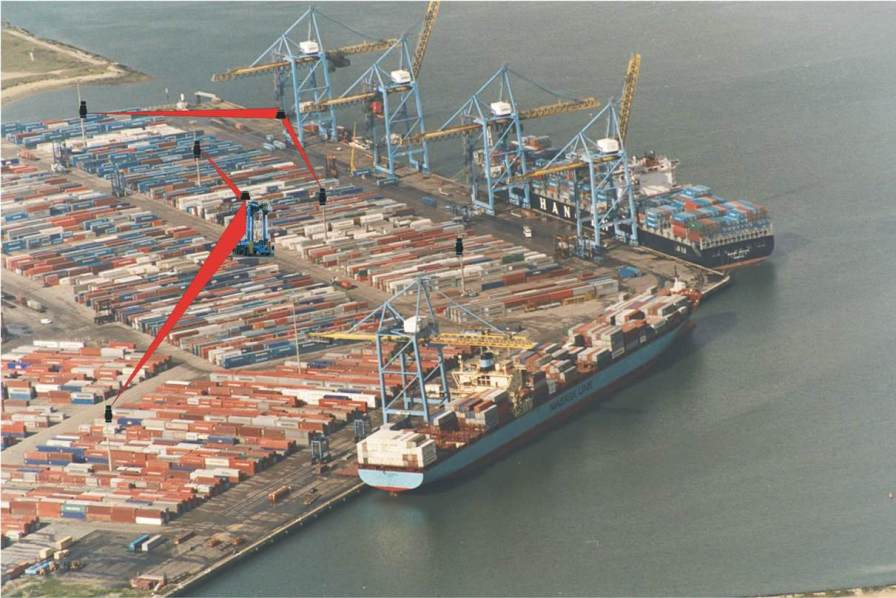
\includegraphics[width=0.6\textwidth]{./chapitres/simulation/bornesLaser.jpg}
  \caption{Réseau de bornes laser implantées sur le Terminal de Normandie (source : \href{http://www.ldtt-fr.com}{http://www.ldtt-fr.com})}
  \label{fig:bornesLaser}
\end{figure}

\begin{figure}[ht]
\centering
 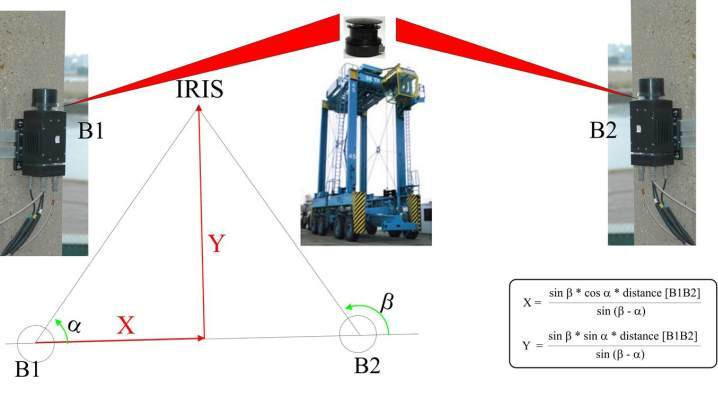
\includegraphics[width=0.6\textwidth]{./chapitres/simulation/triangularisationLaser.jpg}
  \caption{Triangularisation du signal infrarouge entre les bornes IRIS du terminal et celle d'un chariot cavalier (source : \href{http://www.ldtt-fr.com}{http://www.ldtt-fr.com})}
  \label{fig:triangularisation}
\end{figure}

Après plusieurs années de développement et de tests réels, cette technologie se montre performante et fiable et permet de connaître en temps réel la position des engins de manutention au sein du terminal. Cette information est la condition \textit{sine qua non} à toute recherche d'optimisation dynamique des activités des engins de manutention. Grâce à la position des véhicules il est ainsi possible d'optimiser dynamiquement le routage des chariots cavaliers et de prendre en compte les durées de parcours au sein du terminal. Ceci permet par conséquent, d'optimiser l'activité des chariots cavaliers tout en contrôlant le suivi de leurs opérations. En effet, lorsqu'un conteneur est chargé ou déposé par un chariot cavalier, un signal contenant la position du véhicule est envoyé au système. Ainsi, le système connaît la position de prise du conteneur (et par conséquent le conteneur chargé) ainsi que sa position de dépose. Ces informations permettent d'éviter les pertes de conteneurs au sein du terminal.

La partie LITIS du projet consistait à proposer des méthodes d'optimisation dynamique des activités des chariots cavaliers en utilisant l'information fournie par le système de géolocalisation laser. 


	%%%%%%%%%%
	\section{Spécifications}\label{partie:simulation-specification}
	% Spécifications du simulateur

\subsection{Technologie}

Le simulateur est écris en JAVA. Cette technologie a été choisie pour sa souplesse et sa puissance. Elle permet le développement du c\oe{}ur de l'application, de la vue et du contrôleur et assure l'interopérabilité des systèmes et des plates-formes. Une base de données MySQL est également utilisée afin de permettre la communication avec l'interface 3D de notre partenaire \textit{EADS Astrium}. L'accès en écriture et en lecture à cette base est réalisé  par un service web. Le terminal étant constitué de multiples entités en fortes interactions, les calculs sont distribuables sur plusieurs unités grâce à la technologie \textit{RMI} de JAVA.


\subsection{Objectifs}

Le simulateur doit permettre de représenter la structure d'un terminal à conteneurs (blocs, travées, emplacements, carrefours, routes, quais, voies ferrées, etc.) ainsi que ses composants (portiques de berge, portes conteneurs, chariots cavaliers, etc.). Il doit également permettre de modéliser son activité (arrivée/départ des clients (camions, trains, navires), déplacement de conteneurs par les chariots cavaliers, chargement/déchargement des clients par les chariots cavaliers et les portiques). Pour cela, le temps doit être pris en compte par le simulateur. Il a été décidé de discrétiser la représentation du temps dans le simulateur pour être en mesure de se soustraire de l'influence de la (ou les) machine(s) d'exécution et pour synchroniser efficacement les composants. Un pas de temps devra être déterminé avant le début de chaque simulation et déterminera à la fois la précision temporelle et la durée des calculs de la simulation.

\subsection{Flexibilité}

Afin de permettre de mesurer la performance de plusieurs méthodes d'optimisation, le simulateur doit être adapté au développement de ce multiples algorithmes. Il doit permettre d'ajouter, de modifier ou de supprimer rapidement et facilement une méthode d'optimisation. De même, les données concernant les composants et la structure du terminal doivent être aisément modifiables. Ainsi, il a été choisit de décrire toutes les données nécessaire à la fois à la configuration du programme et aux composants du terminal dans des fichiers XML dont la structure est décrite dans les sections suivantes.


	%%%%%%%%%%
% 	\section{Architecture}\label{partie:simulation-architecture}
	% Section Architecture du Simulateur


\section{Modélisation du système}

Un terminal portuaire à conteneurs est un système complexe. En effet, on peut définir un système complexe comme un groupe très important d'entités en interactions et dont le comportement ne peut pas, à lui seul, définir l'état futur du système. De plus, ce système est ouvert sur l'extérieur, il est donc soumis à des flux entrant et sortant d'information générant des perturbations sur l'état du système. Un terminal portuaire peut alors être vu comme la superposition de plusieurs sous-systèmes en interactions les uns avec les autres. Parmi ces sous-systèmes on trouve le réseau routier, les espaces de stockages, les véhicules ainsi que leur système de mobilité, et enfin les éléments stockés c'est-à-dire les conteneurs. Le simulateur a donc pour objectif de modéliser le plus fidèlement possible ces éléments ainsi que leurs interactions.

\subsection{Graphe routier}

Les carrefours et les routes composant le réseau routier du terminal décrivent un graphe $G=(V,A)$ où $V$ est l'ensemble des sommets et $A$ est l'ensemble des arcs. Les arcs sont orientés et lorsque la circulation d'un véhicule est possible dans les deux sens entre deux carrefours $v_i$ et $v_j$ alors il existe deux arcs $(v_i,v_j)$ et $(v_j,v_i)$. Chaque arc du graphe comporte un poids modélisant la distance séparant les deux sommets de l'arc. Un carrefour routier permet de relier au moins deux routes.

Afin de modéliser des routes sinueuses, la notion de point de route a été introduite. Un point de route est un sommet permettant de relier deux arcs d'une même route. Ainsi une même route comporte 2 carrefours et $n$ points de routes. Ce procédé permet de simplifier le calcul des plus court chemins en réduisant le nombre d'arcs dans le graphe.

La figure \ref{fig:simulation:grapheRoutier} montre la vue d'une partie du graphe routier d'un terminal dans le simulateur.

\begin{figure}[h]
 \centering
 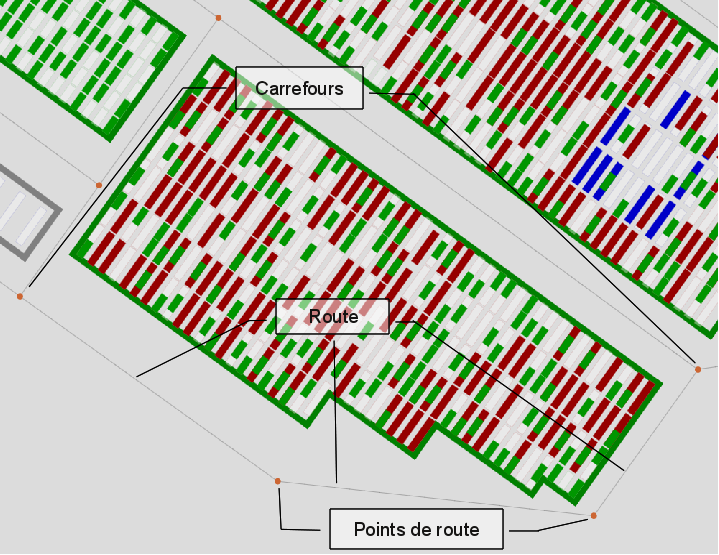
\includegraphics[width=0.6\textwidth]{chapitres/simulation/grapheRoutier.png}
 \caption{Exemple de routes comportant des points de route sur le Terminal de Normandie}
 \label{fig:simulation:grapheRoutier}
\end{figure}

Les travées sont des routes réservées aux chariots cavaliers sur lesquelles ces engins ne peuvent pas se croiser. Une travée est modélisée par un arc First In, First Out (FIFO) relié aux routes par des points de travées. Un point de travée est un point de route reliant à la fois deux arcs et une ou plusieurs travées. Avec cette modélisation il est possible de représenter le réseau routier de n'importe quel terminal à conteneurs.

\subsection{Réseau de stockage}

Avant le début du projet CALAS, le terminal était composé de 2 principaux sous-systèmes. D'une part le réseau routier permettant aux véhicules de se déplacer à l'intérieur du terminal et d'autre part le réseau de stockage. Ce dernier est composé de 3 zones (voir fig. \ref{fig:simulation:3zones}) :
\begin{itemize}
 \item La \textbf{zone maritime} (\textit{Quay side}) permettant de charger ou de décharger la cargaison des navires;
 \item La \textbf{zone de stockage interne} (\textit{Yard}) dédiée au stockage temporaire des conteneurs en attente de transit;
 \item La \textbf{zone terrestre} (\textit{Land side}) permettant de charger ou de décharger la cargaison des véhicules terrestres, c'est-à-dire des camions et des trains.
\end{itemize}

\begin{figure}[h]
 \centering
 \includegraphics[width=0.6\textwidth]{chapitres/simulation/3zonesDuTN.png}
 \caption{Les 3 types de zones du Terminal de Normandie}
 \label{fig:simulation:3zones}
\end{figure}

Chacune des zones est en interaction avec le réseau routier et comporte différents type d'engins de manutention. Des grues de quai sont utilisées dans la zone maritime pour charger/décharger les navires. Dans le cas d'un déchargement, les conteneurs sont posés sur le quai par la grue puis un chariot cavaliers se charge de transporter le conteneur vers sa destination, c'est-à-dire soit la zone de stockage, soit la zone terrestre, ou soit, dans le cas d'un cabotage, à un autre endroit sur la zone maritime. Dans le cas d'un chargement c'est le chariot cavalier qui amène le conteneur au pied de la grue. Concernant la zone de stockage et la zone terrestre, ce sont les chariots cavaliers qui sont affectés directement au chargement/déchargement des camions ou des trains et au transport des conteneurs entre les zones. Ces véhicules sont capables de transporter un conteneur sur 3 voire 4 niveaux pour les plus récents. Ils peuvent ainsi se déplacer avec un conteneur dans une travée de 3 étages pour les meilleurs et 2 étages pour les autres.

Chaque zone est composée de pavés. Un pavé (ou bloc) est un regroupement de travées de conteneurs. Chaque pavé comporte donc un certain nombre de travées. Une travée est reliée au réseau routier par des points de travée et représente donc une route particulière qui ne peut être empruntée que par les chariots cavaliers. Elles comportent une série d'emplacements de différentes longueurs pour stocker les conteneurs. Les emplacements où se garent les camions pour être chargés/déchargés sont ainsi modélisés par une travée ne comportant qu'un seul emplacement. Les wagons de trains sont eux aussi modélisés par des travées ne pouvant contenir qu'un seul étage de conteneurs. Pour ces deux types de véhicules, les emplacements sont disponibles si le camion ou le train est en place. Dans le cas contraire, les chariots cavaliers ne peuvent effectuer le chargement ou le déchargement du conteneur.

\subsection{Système de géolocalisation laser (LDTT)}

Suite au projet CALAS, le terminal de Normandie s'est vu doté d'un troisième sous-système : la géolocalisation des engins de manutention. En effet, un réseau de bornes laser a été déployé sur le terminal dans le but de mesurer avec précision la position des véhicules. Ces bornes communiquent avec un serveur central afin de transmettre les coordonnées des chariots. Ce système a été modélisé en simulant la détection des chariots par les bornes selon une certaine portée. Une fois détecté, la borne laser envoie la position du véhicule au système central qui mets à jour les informations connues sur ce chariot. De cette façon, si un véhicule se trouve en dehors de la couverture du réseau de bornes laser, le système ne reproduit que sa dernière position connue. La figure \ref{fig:simulation:laser} montre une la vue 2D du Terminal de Normandie dans le simulateur, et où chaque cercle représente la portée d'une borne laser.

\begin{figure}[h]
 \centering
 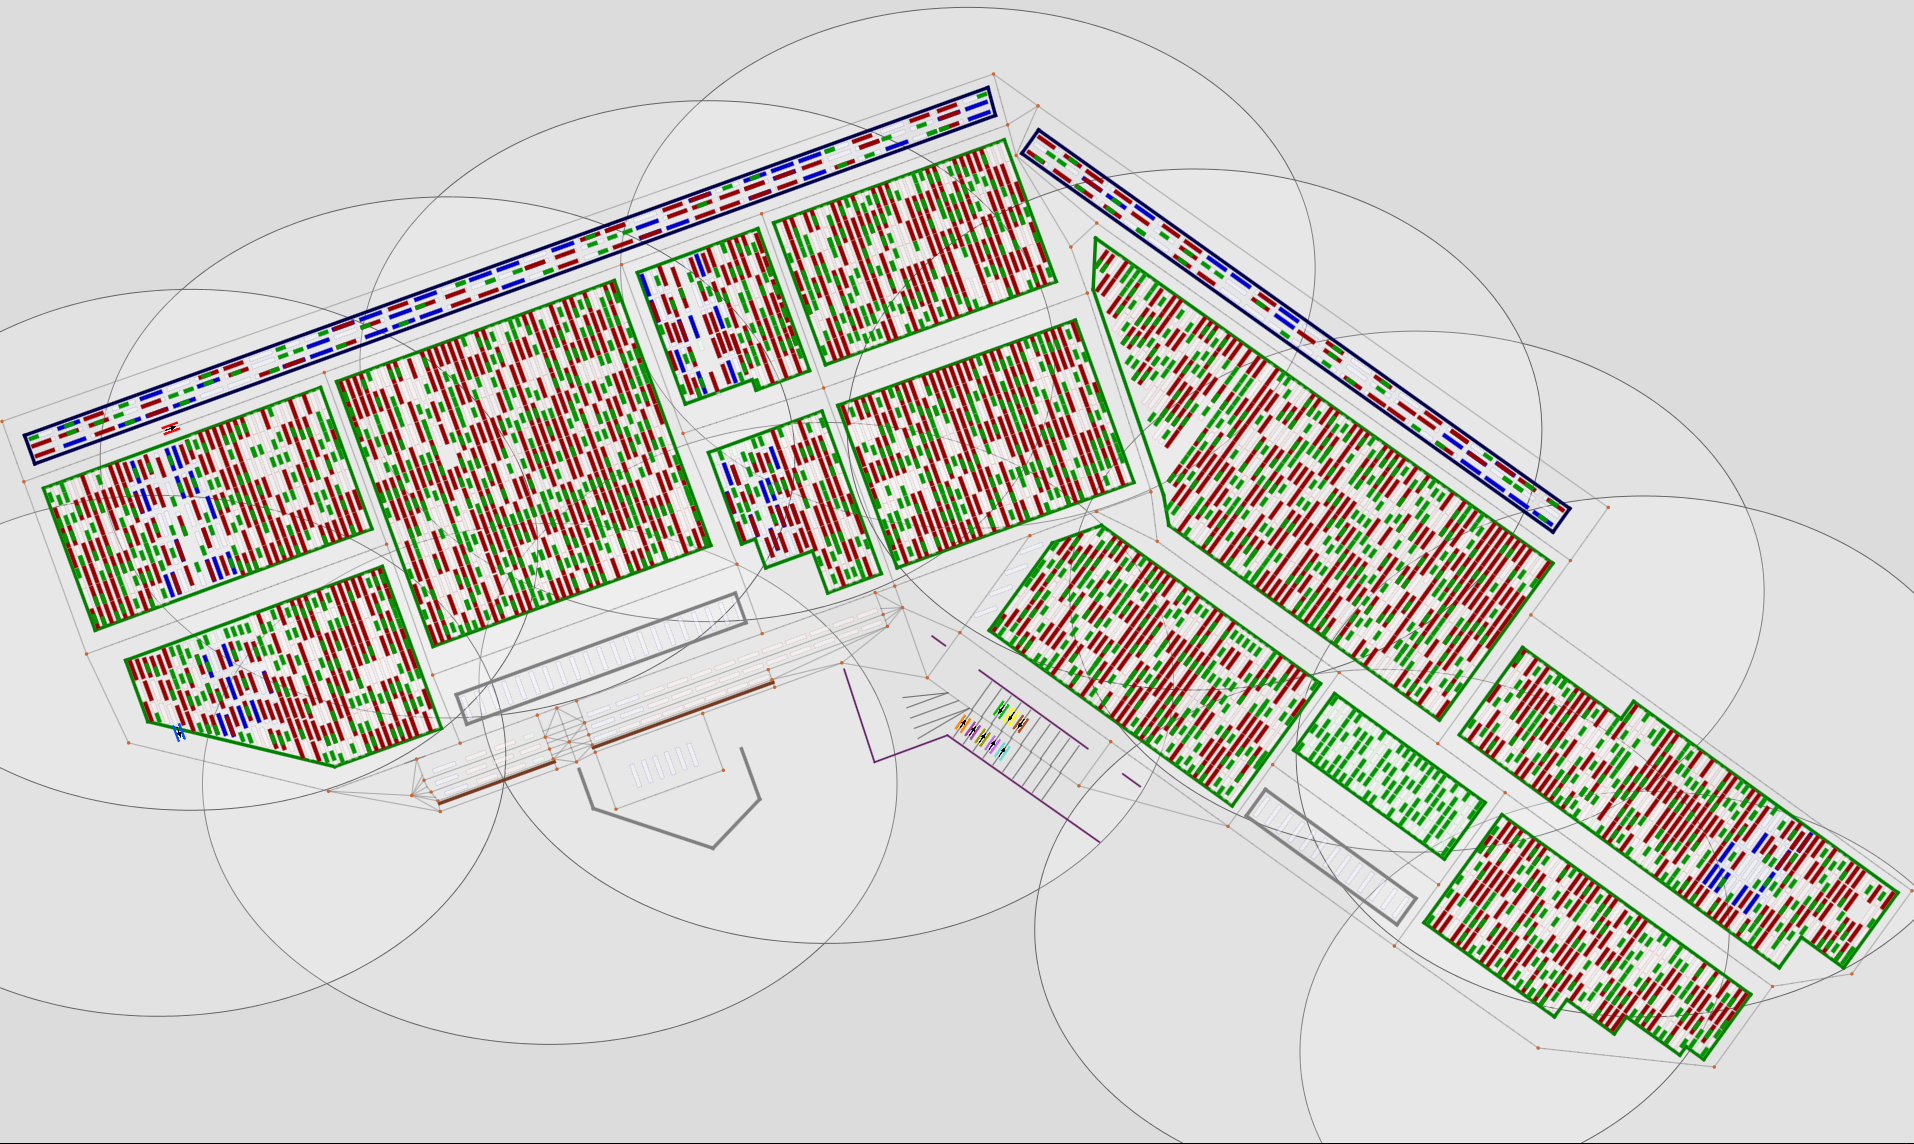
\includegraphics[width=0.8\textwidth]{chapitres/simulation/captureBornesLaser.png}
 \caption{Vue 2D du simulateur montrant le Terminal de Normandie ainsi que le système de localisation laser}
 \label{fig:simulation:laser}
\end{figure}

\subsection{Mobilité au sein du terminal}

Dans la modélisation choisie ici, seuls les chariots cavaliers sont mobiles. En effet, ils sont les seuls véhicules à pouvoir déplacer les conteneurs au sein du terminal. La mobilité des autres véhicules (navires, camions et trains) ne comporte que les actions d'arrivée et de départ. Ainsi, un camion est soit sur son emplacement de chargement/déchargement, soit en dehors du terminal. Toutefois, d'autres véhicules peuvent être ajoutés facilement en décrivant leur comportement dans le
simulateur. 

Les chariots cavaliers sont donc les seuls véhicules à pouvoir emprunter les travées de conteneurs. Cependant, ils ne peuvent pas se croiser à l'intérieur de celles-ci. C'est cet élément qui caractérise les arcs (ou arêtes) de type travée. En effet, les travées sont \textit{First-In-First-Out} (premier entré, premier sorti), c'est-à-dire que les véhicules sortent de la travée dans le même ordre qu'ils y sont entrés. Pour éviter des blocages, les chariots cavaliers n'ont pas l'autorisation d'emprunter une travée déjà occupée par un autre chariot. Si la travée est prise, ils devront attendre à l'entrée de celle-ci jusqu'à ce qu'elle soit libérée.

Sur les routes, les chariots peuvent se croiser et se doubler. Néanmoins, les dépassements ne sont pas modélisés fidèlement, c'est-à-dire que les différentes voies de circulation ne sont pas modélisées et que les collisions ne sont pas prises en compte. Ce procédé permet de simplifier la modélisation sans pour autant dégrader la qualité de la simulation. En effet, suite à une collision, les véhicules deviendront simplement indisponibles (en panne) durant un certain temps.

Le comportement des conducteurs des chariots est complexe à reproduire. En théorie, ces derniers choisissent une mission à effectuer parmi celles que le système leur propose et se rendent sur les emplacements de collecte et de livraison de conteneurs selon l'itinéraire affecté par le système. En réalité les conducteurs s'échangent des missions entres eux et choisissent leur propre itinéraire. Ces comportements ont été modélisés par des événements de non respect d'affectation et d'itinéraire. De cette façon, il est possible d'introduire de la dynamicité dans la simulation et surtout de pouvoir la quantifier facilement.

\subsection{Temporalité}

L'objectif étant d'étudier l'impact de la dynamicité sur l'évolution du système, la modélisation du temps est essentielle. Il a été décidé de se placer dans le cas discret, avec un pas de temps réglable. Ainsi, il est possible de modéliser les événements liés à la dynamique.

Le simulateur permettant de préciser le pas de temps pour une simulation, il sera possible d'étudier l'influence du choix du pas de temps sur les résultats des simulations au niveau macro. La figure \ref{fig:simulation:temporalite} montre deux captures d'écran d'une simulation à 1 pas de temps d'intervalle. Ici le véhicule mauve situé dans le quart inférieur droit de l'image continue son déplacement. La vitesse du véhicule étant de 27km/h, il aura effectué 15 mètres pendant les 2 secondes simulées.

\begin{figure}[h]
  \centering
  \begin{tabular}{c}
    \subfloat[Capture d'écran du simulateur à t=3m33s]{\label{subfig:capture1}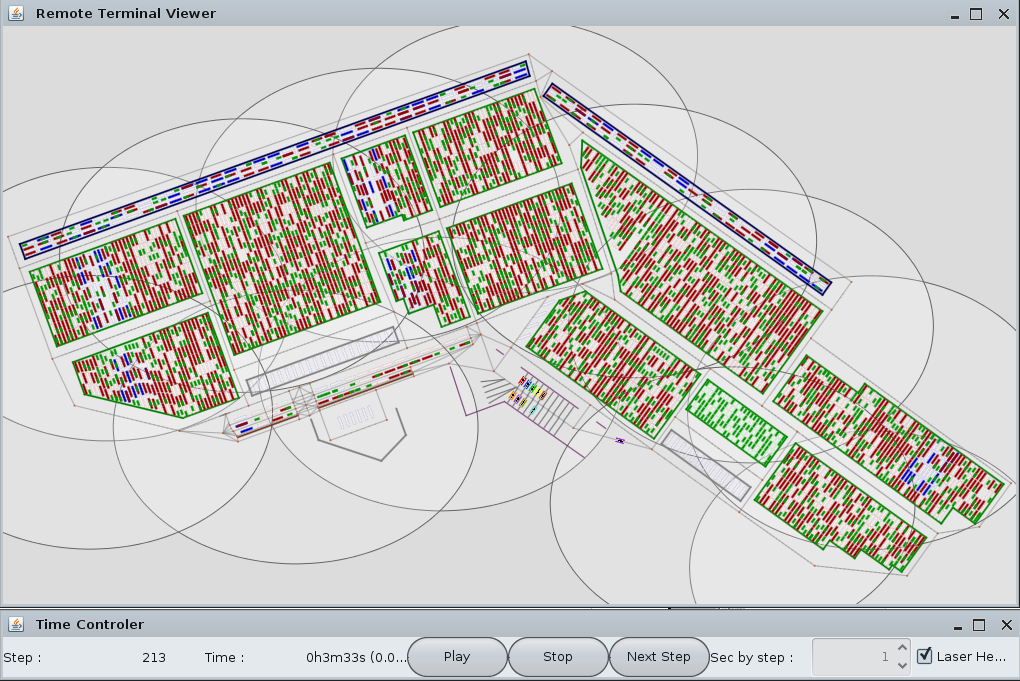
\includegraphics[width=0.9\textwidth]{chapitres/simulation/capture3m33s.png}} \\
    \subfloat[Capture d'écran du simulateur à t=3m35s]{\label{subfig:capture2}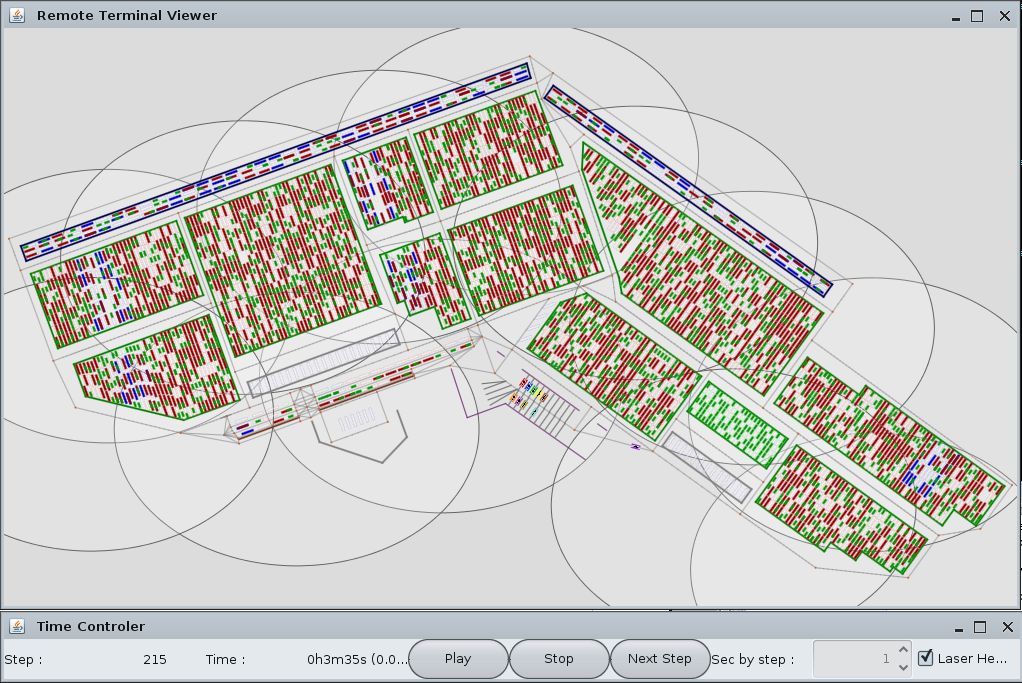
\includegraphics[width=0.9\textwidth]{chapitres/simulation/capture3m35s.png}} \\
  \end{tabular}
  \caption{Exemple de représentation discrète du temps, ici avec un pas de temps de 2 secondes par itération}
  \label{fig:simulation:temporalite}
\end{figure}

\FloatBarrier

\subsection{Événements}

Les événements interviennent au cours du temps et possèdent donc un marqueur temporel de déclenchement. Il existe des événements de différentes natures :
\begin{itemize}
 \item arrivée de mission : une nouvelle mission est connue du système;
 \item annulation de mission : une mission déjà connue est retirée du système;
 \item arrivée de véhicule (bateau, camion, train) : un véhicule est arrivé sur son/ses emplacements;
 \item départ de véhicule (bateau, camion, train) : un véhicule a quitté son/ses emplacements;
 \item panne de chariot cavalier : un chariot est indisponible;
 \item fin de panne de chariot cavalier : un chariot indisponible redevient disponible;
 \item non respect d'affectation de mission d'un chariot cavalier : le conducteur d'un chariot a choisi une mission qui ne lui était pas destinée;
 \item non respect d'itinéraire d'un chariot cavalier : le conducteur d'un chariot a choisi un itinéraire différent de celui proposé par le système;
 \item perte de conteneur : un conteneur ne se trouve pas à l'emplacement indiqué par le système.
\end{itemize}

L'objectif est de reproduire un terminal portuaire à conteneurs tant dans son contenu que dans son comportement. Chaque sous-système du terminal a donc été modélisé ainsi que les interactions, à la fois à l'intérieur et entre ces sous-systèmes.
 
\section{Collecte des données}

Une fois le modèle établi, il est nécessaire de collecter des données afin de décrire un terminal existant. Le choix s'est porté sur le Terminal de Normandie, un des terminaux du Port Autonome du Havre directement impliqué dans le projet CALAS.

La difficulté rencontrée quant à l'obtention d'information concernant les données du terminal est l'une des raisons pour lesquelles le développement d'un simulateur a été la solution retenue pour de mettre au point et tester la performance de nos méthodes. Une grande partie du temps alloué au projet a donc été consacré à la collecte d'informations sur : 
\begin{itemize}
 \item Les chariots cavaliers : dimensions, vitesse, comportement;
 \item Le fonctionnement du terminal : différentes zones d'échange, zone de stockage, engins de manutention;
 \item Le réseau routier du terminal : 
  \begin{itemize}
   \item coordonnées des carrefours;
   \item routes;
   \item travées;
   \item coordonnées des emplacements conteneurs dans les travées;
   \item zone de dépôt des engins de manutention.
  \end{itemize}
\end{itemize}

Les coordonnées des carrefours, routes, travées et emplacements conteneurs du Terminal de Normandie ont été obtenus grâce à un plan sommaire du terminal fourni par nos partenaires du projet CALAS (voir figure \ref{fig:planTerminalSommaire}) et au site internet de cartographie \href{http://wikimapia.org/\#lat=49.4694697\&lon=0.1676486\&z=16\&l=2\&m=b}{wikimapia.org}. Ce site permet de mesurer de façon relativement précise des distances sur des photos satellites d'une grande définition. Les coordonnées indiquées sur le plan fourni par nos partenaires sont exprimés en suivant la projection conique conforme de Lambert (zone centre : Lambert II). Un degré de ce système correspond à 100km. Cette équivalence permet de calculer aisément les coordonnées des points manquant du plan grâce aux distances mesurées sur le site \href{http://wikimapia.org/\#lat=49.4694697\&lon=0.1676486\&z=16\&l=2\&m=b}{wikimapia.org}.

\begin{figure}[ht]
\centering
 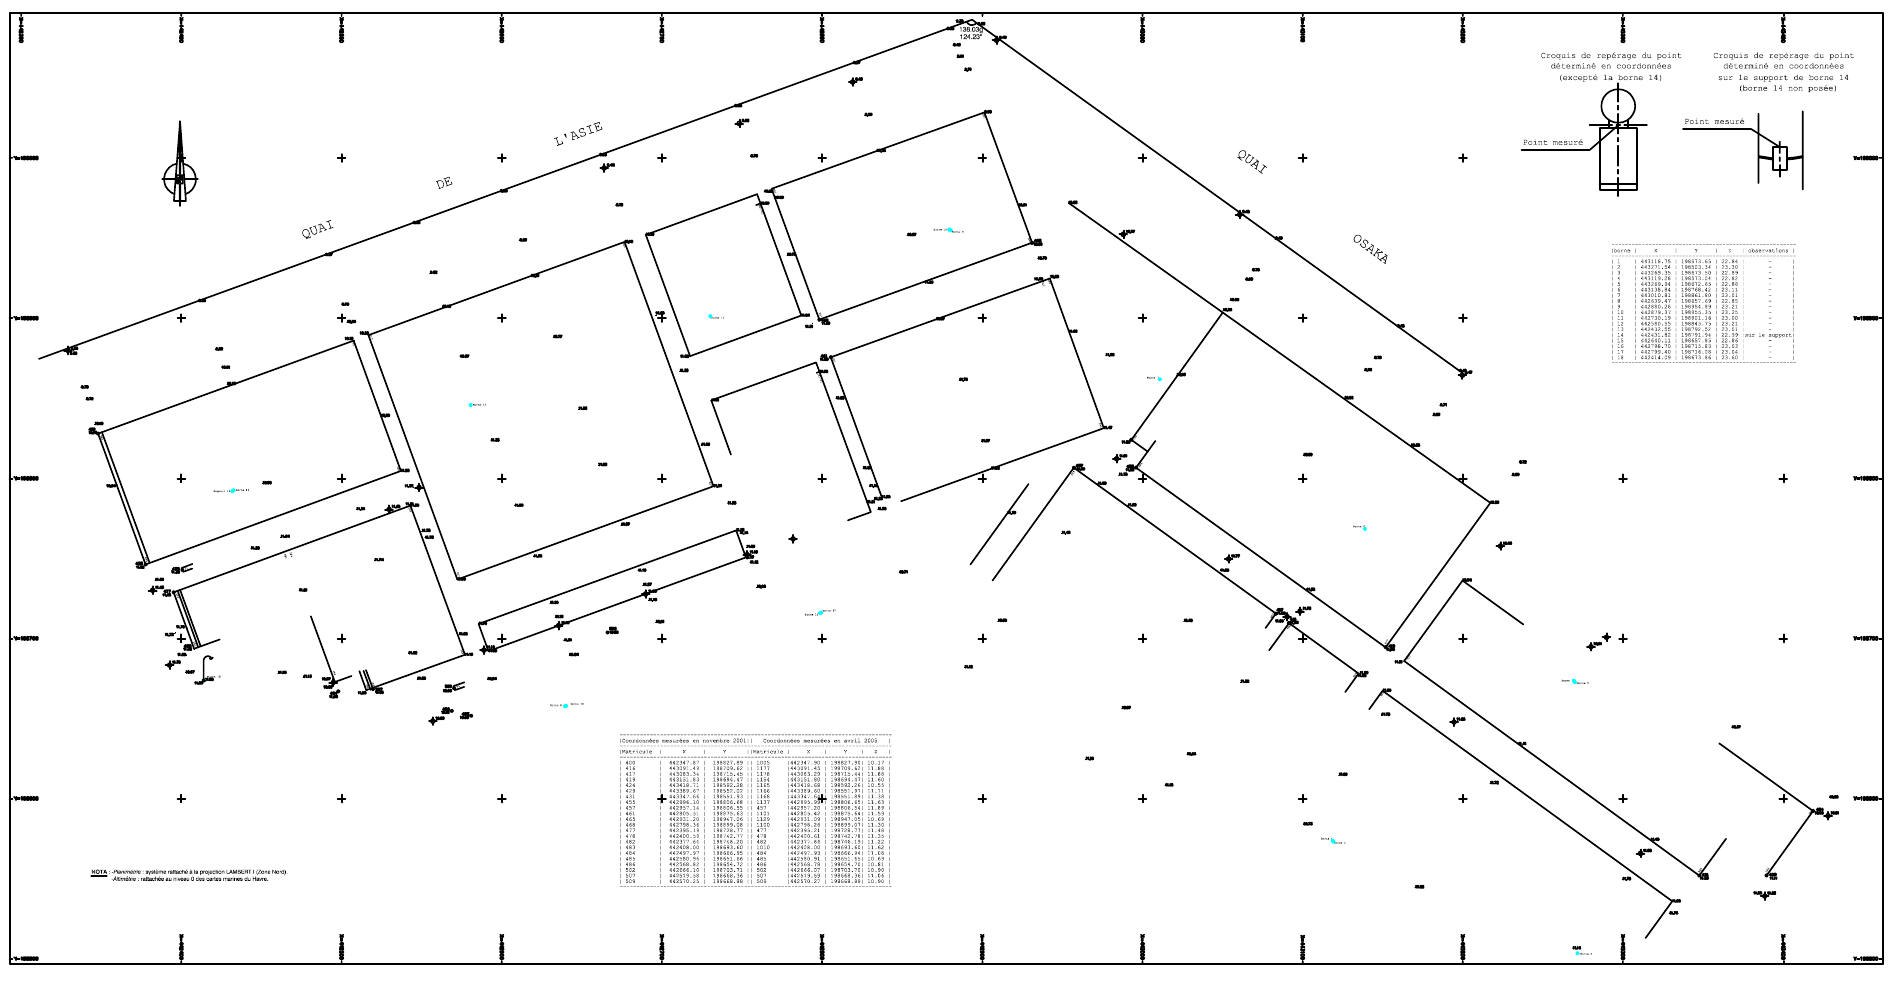
\includegraphics[width=0.8\textwidth]{./chapitres/simulation/planTerminalSommaire.png}
  \caption{Plan sommaire du Terminal de Normandie}
  \label{fig:planTerminalSommaire}
\end{figure}

La figure \ref{fig:planTerminalComplet} montre le plan obtenu grâce aux recroisemment des informations du plan sommaire et de \href{http://wikimapia.org/\#lat=49.4694697\&lon=0.1676486\&z=16\&l=2\&m=b}{wikimapia.org}. Le Terminal de Normandie, loin d'être le plus grand au monde, comporte tout de même 1170 carrefours, 170 routes, 531 travées et 3499 emplacements conteneurs.

\begin{figure}[ht]
\centering
 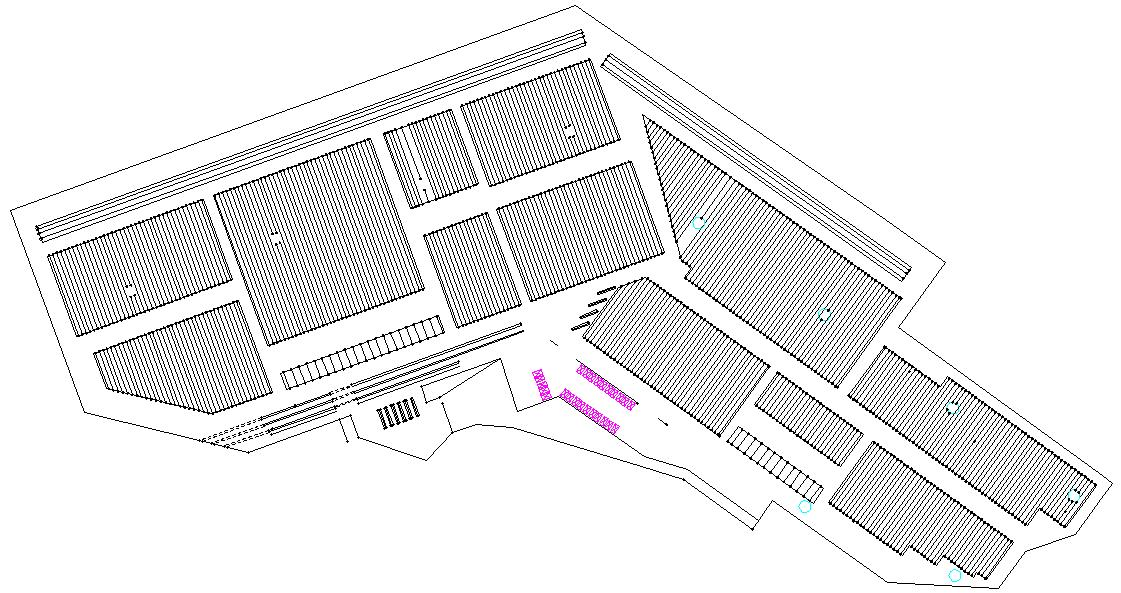
\includegraphics[width=0.8\textwidth]{./chapitres/simulation/planTerminalComplet.jpg}
  \caption{Plan du Terminal de Normandie obtenu après collecte et recoupement des données}
  \label{fig:planTerminalComplet}
\end{figure}

D'autre part, les images satellites ont également permis de collecter des données sur les chariots cavaliers et notamment leur lieu de stationnement (dépôt). Des données concernant les chariots
cavaliers ont également été récupérées sur les sites des constructeurs afin de connaître leurs principales dimensions :
\begin{itemize}
 \item longueur hors tout ;
 \item largeur hors tout ;
 \item hauteur hors tout ;
 \item longueur des panneaux latéraux ;
 \item largeur interne (entre les deux panneaux latéraux) ;
\end{itemize}

ainsi que des informations sur la vitesse moyenne de fonctionnement, les temps de manutention, etc. Toutes ces informations sont décrites dans des fichiers au format \verb!XML!.

\section{Structuration des données}\label{sec:structurationDonnees}

Les données des simulations sont décrites dans des fichiers \verb!XML!. L'Extensible Markup Language (langage extensible de balisage 5) permet de définir de façon lisible des caractéristiques et des comportements dans de simple fichiers texte et sont également rapidement interprétables par le programme. Il existe différents fichiers de configurations nécessaires au fonctionnement du simulateur :
\begin{itemize}
 \item le fichier de déploiement de l'application;
 \item le fichier de configuration du système de localisation laser (position et portée des bornes);
 \item le fichier de description des véhicules;
 \item le fichier de configuration du terminal (zones de stockage, réseau routier);
 \item le fichier d'initialisation du terminal permettant de décrire la position des conteneurs au démarrage de la simulation;
 \item les fichiers d'événements (missions, pannes de véhicule ou de borne laser, arrivées ou départs des véhicules clients, etc).
\end{itemize}

\subsection{Réseau routier}\label{sec:description:resRoutier}

Les routes et les carrefours d'un terminal portuaire à conteneurs constituent un graphe. Ainsi, les n\oe{}uds du graphe sont des carrefours et les routes sont des arcs. La structure \verb!XML! doit donc permettre de décrire ce graphe. Les coordonnées sont exprimées en mètres selon la projection conique de Lambert.

\begin{figure}[h]
 
\begin{lstlisting}[language=XML]
  <crossroad id='' x='' y=''/>
  <road
    id=''
    origin='crossroadId'
    destination='crossroadId'
    [directed='boolean']
  />
\end{lstlisting}
\caption{Code XML nécessaire à la description d'un carrefour et d'une route}
\label{fig:simulation:carrefourRoute}
\end{figure}

Un arc étant représenté par une droite entre deux n\oe{}uds, l'objet roadpoint (point de route) a été introduit pour permettre de modéliser des routes sinueuses. Ainsi une route est une liste d'arcs dont le premier part d'un n\oe{}ud et le dernier se termine par un autre n\oe{}ud. Tous les autres arcs de cette route relient des points de route. La figure \ref{fig:simulation:ptsRoute} donne un exemple de code \verb!XML! décrivant une route reliant le carrefours A au carrefour B et utilisant deux points de route, ainsi que le graphe ainsi généré.

\begin{figure}[h]
 
\begin{lstlisting}[language=XML]
<crossroad id='A' x='0' y='1' > </crossroad>
<crossroad id='B' x='3' y='1' > </crossroad>
<road id=' ' origin='A' destination='B'>
<roadpoint id='C' x='1' y='2' > premier point </roadpoint>
  <!--... autres points de route eventuels -->
<roadpoint id='D' x='2' y='0' > dernier point </roadpoint>
</road>
\end{lstlisting}

{
\centering
\tikzstyle{vertex}=[circle,draw,fill=white,line width=0.5pt,minimum size=25pt,inner sep=0pt,font=\tiny]
\tikzstyle{edge} = [draw,thick,->]
 \begin{tikzpicture}[xscale=3, yscale=0.5, auto,swap]
     \foreach \pos/\name in {
	{(0,1)/A},
	{(3,1)/B}, {(1,2)/C},
	{(2,0)/D}}
      \node[vertex] (\name) at \pos {$\name$};

    \foreach \source/ \dest in {A/C, C/D, D/B} \path[edge] (\source) node[] {} -- node[] {} (\dest);
\end{tikzpicture}\\
}
\caption{Exemple de description XML d'un arc comportant des points de route}
\label{fig:simulation:ptsRoute}
\end{figure}

\subsection{Zones de stockage}\label{sec:description:zonesStockage}

Il existe deux types de zones sur un terminal à conteneurs. D'une part, les zones d'échanges (quais, zone ferroviaire et zone routière) et les zones de stockage d'autre part. Une zone est modélisée par la balise \verb!<pave id='' type='{BOAT, ROAD, TRAIN, STOCK}'>! \verb!</pave>!. À l'intérieur de cette balise se trouvent les coordonnées des contours de la zone. La balise \verb!<wall from='' to=''>! \verb!</wall>! permet de relier ces points.

\begin{subfigures}
\begin{figure}
\centering
 \begin{lstlisting}[language=XML]
<pave id="L" type="ROAD">
<coordinate id="L-NW" x="443051.6250" y="198654.4978"/>
<coordinate id="L-NE" x="443138.2976" y="198591.7532"/>
<coordinate id="L-SE" x="443127.3772" y="198576.6273"/>
<coordinate id="L-SW" x="443040.6241" y="198639.2604"/>
<wall from="L-NW" to="L-NE"/>
<wall from="L-NE" to="L-SE"/>
<wall from="L-SE" to="L-SW"/>
<wall from="L-SW" to="L-NW"/>
</pave>
\end{lstlisting}
\caption{Code XML d'une zone de chargement/déchargement de camions}
\end{figure}

\begin{figure}[h]
  \centering
  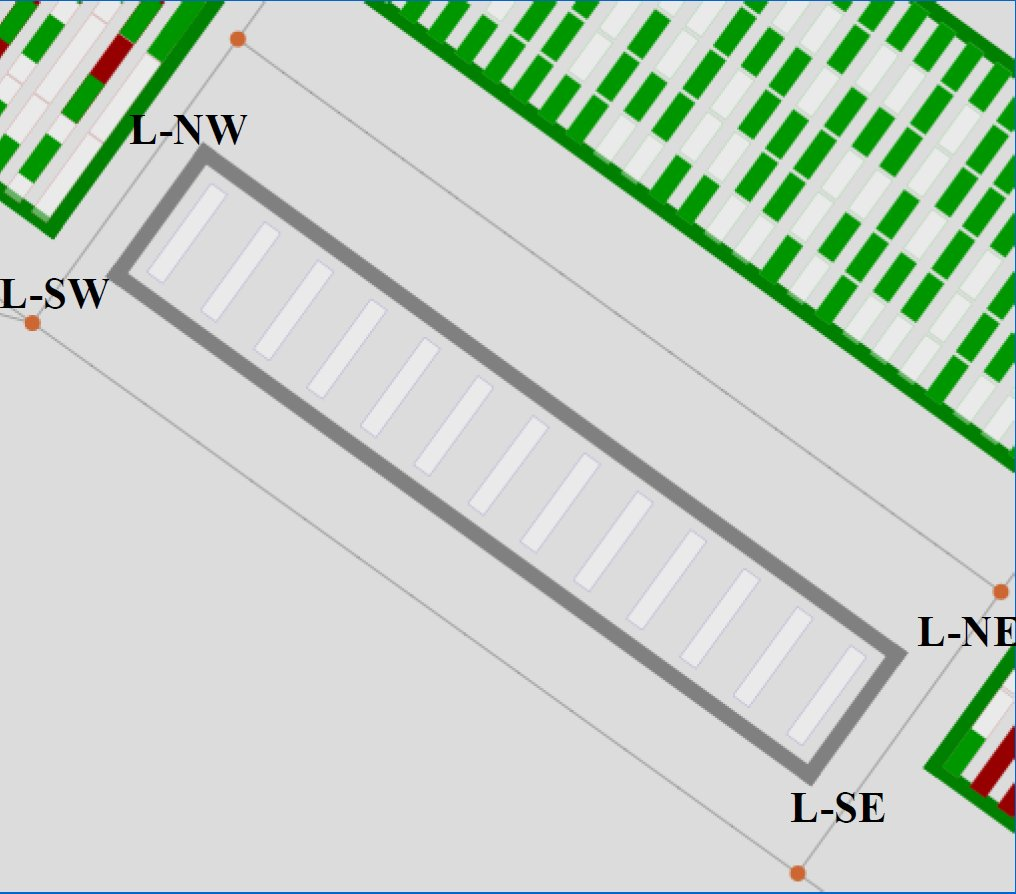
\includegraphics[width=0.75\textwidth]{chapitres/simulation/pave.jpg}
  \caption{Rendu 2D de cette zone dans $D^2CTS$ }
\end{figure}
\label{fig:simulation:pave}
\end{subfigures}

Les travées sont également décrites à l'intérieur de la balise \verb!<pave>! de la zone concernée. Les points d'entrée et de sortie des travées sur les routes sont des points de routes spécifiques décrits par la balise \verb!<laneCrossroad>! et sont insérés à l'intérieur de la balise \verb!<road>! de la route permettant d'accéder à la travée.
La balise \verb!<lane id='' origin='' destination='' slots=''>! permet de décrire une travée grâce à l'identifiant, le point d'entrée, le point de sortie et la description des emplacements conteneurs de cette travée. Cette dernière information est donnée sous la forme : $tailleConteneurEnPieds*nombreD'emplacementsDeCetteTaille$

Par exemple, une travée comportant 2 emplacements de 40 pieds puis 1 emplacement de 20 pieds sera décrite en \verb!XML! de la façon suivante :
\begin{lstlisting}[language=XML]
<lane id='' origin='' destination='' slots='40*2-20*1'/>
\end{lstlisting}

De plus, les coordonnées du premier et du dernier emplacement de la travée peuvent être précisées grâce aux paramètres \verb!in='coordX,coordY'! et \verb!out='coordX,coordY'!. Dans le cas contraire, ces coordonnées sont calculées de façon à conserver la même distance entre les conteneurs ainsi qu'entre le premier emplacement et le point d'entrée de la travée et entre le dernier emplacement et le point de sortie de la travée. Si les coordonnées \verb!in! et \verb!out! sont précisées alors les emplacements contenus entre le premier et le dernier sont répartis de façon régulière entre ces deux emplacements. 
Les emplacements de trains et de camions sont modélisés par des travées spécifiques. Ces travées sont décrites par la balise \verb!<exchangeLane>! en \verb!XML!. Les paramètres sont les mêmes que pour une travée classique (\verb!<lane>!). La figure \ref{fig:simulation:travee} donne un exemple d'utilisation de ces balises.

\begin{figure}[ht]
\centering
 \begin{lstlisting}[language=XML]
<pave id="L" type="ROAD">
<coordinate id="L-NW" x="443051.6250" y="198654.4978"/>
<coordinate id="L-NE" x="443138.2976" y="198591.7532"/>
<coordinate id="L-SE" x="443127.3772" y="198576.6273"/>
<coordinate id="L-SW" x="443040.6241" y="198639.2604"/>
<wall from="L-NW" to="L-NE"/>
<wall from="L-NE" to="L-SE"/>
<wall from="L-SE" to="L-SW"/>
<wall from="L-SW" to="L-NW"/>
<road id="c32-c38" origin="c32" destination="c38">
<laneCrossroad id="L_S_1" x="443037.4695" y="198627.9259"/>
<laneCrossroad id="L_S_2" x="443044.1513" y="198623.1196"/>
<laneCrossroad id="L_S_3" x="443050.8331" y="198618.3134"/>
<laneCrossroad id="L_S_4" x="443057.5149" y="198613.5071"/>
<laneCrossroad id="L_S_5" x="443064.1967" y="198608.7009"/>
<laneCrossroad id="L_S_6" x="443070.8785" y="198603.8946"/>
<laneCrossroad id="L_S_7" x="443077.5602" y="198599.0884"/>
<laneCrossroad id="L_S_8" x="443084.2420" y="198594.2822"/>
<laneCrossroad id="L_S_9" x="443090.9238" y="198589.4759"/>
<laneCrossroad id="L_S_10" x="443097.6056" y="198584.6697"/>
<laneCrossroad id="L_S_11" x="443104.2874" y="198579.8634"/>
<laneCrossroad id="L_S_12" x="443110.9692" y="198575.0572"/>
<laneCrossroad id="L_S_13" x="443117.6509" y="198570.2510"/>
</road>
<exchangeLane id="L-1/13" origin="L_N_1" destination="L_S_1" slots="45*1" in="443054.9578,198652.0845" out="443043.9608,198636.8514"/>
<exchangeLane id="L-2/13" origin="L_N_2" destination="L_S_2" slots="45*1" in="443061.6258,198647.2580" out="443050.6341,198632.0335"/>
<exchangeLane id="L-3/13" origin="L_N_3" destination="L_S_3" slots="45*1" in="443068.2929,198642.4315" out="443057.3074,198627.2155"/>
<exchangeLane id="L-4/13" origin="L_N_4" destination="L_S_4" slots="45*1" in="443074.9600,198637.6050" out="443063.9807,198622.3976"/>
<exchangeLane id="L-5/13" origin="L_N_5" destination="L_S_5" slots="45*1" in="443081.6271,198632.7785" out="443070.6540,198617.5797"/>
<exchangeLane id="L-6/13" origin="L_N_6" destination="L_S_6" slots="45*1" in="443088.2942,198627.9520" out="443077.3273,198612.7617"/>
<exchangeLane id="L-7/13" origin="L_N_7" destination="L_S_7" slots="45*1" in="443094.9613,198623.1255" out="443084.0007,198607.9438"/>
<exchangeLane id="L-8/13" origin="L_N_8" destination="L_S_8" slots="45*1" in="443101.6284,198618.2990" out="443090.6740,198603.1259"/>
<exchangeLane id="L-9/13" origin="L_N_9" destination="L_S_9" slots="45*1" in="443108.2956,198613.4724" out="443097.3473,198598.3080"/>
<exchangeLane id="L-10/13" origin="L_N_10" destination="L_S_10" slots="45*1" in="443114.9627,198608.6459" out="443104.0206,198593.4900"/>
<exchangeLane id="L-11/13" origin="L_N_11" destination="L_S_11" slots="45*1" in="443121.6298,198603.8194" out="443110.6939,198588.6721"/>
<exchangeLane id="L-12/13" origin="L_N_12" destination="L_S_12" slots="45*1" in="443128.2969,198598.9929" out="443117.3672,198583.8542"/>
<exchangeLane id="L-13/13" origin="L_N_13" destination="L_S_13" slots="45*1" in="443134.9640,198594.1664" out="443124.0405,198579.0362"/>
</pave>
\end{lstlisting}
\caption{Exemple de code XML de description d'une travée}
\label{fig:simulation:travee}
\end{figure}

\FloatBarrier

\subsection{Conteneurs}

Le simulateur tient compte de l'hypothèse selon laquelle il existe 3 types de conteneurs sur le Terminal de Normandie. D'abord les conteneurs de 20 pieds : 1 TEU (twenty feet equivalent unit); les conteneurs de 40 pieds : 2 TEU ; et enfin les conteneurs de 45 pieds : 2.25 TEU qui sont des conteneurs réfrigérés. Les dimensions de ces conteneurs sont les suivantes (normes ISO) :

\begin{center}
\footnotesize
\begin{tabular}{|c|c|c|c|}
  \hline
  \textbf{\textit{Type}} & \textbf{\textit{Longueur (m)}} & \textbf{\textit{Largeur (m)}} & \textbf{\textit{Hauteur (m)}} \tabularnewline
  \hline
  20 pieds & 6,058 & 2,438 & 2,591 \tabularnewline
  \hline
  40 pieds & 12,192 & 2,438 & 2,591 \tabularnewline
  \hline
  45 pieds & 13,716 & 2,438 & 2,896 \tabularnewline
  \hline
\end{tabular}
\end{center}

Pour pouvoir décrire un conteneur en \verb!XML! il faut donner l'identifiant du conteneur et son type (en TEU). Il est également possible de spécifier sa position. Cette dernière est définie par un pavé, une travée, un emplacement, un niveau et enfin un alignement. 
Le niveau correspond à l'étage auquel le conteneur est stocké sur l'emplacement. L'étage 0 correspond au rez-de-chaussé (le conteneur est posé sur le sol du terminal). Il est possible de stocker deux niveaux de conteneurs dans les travées de stockage et un seul niveau sur les trains et les camions.
L'alignement du conteneur permet de définir si le conteneur est centré sur son emplacement, c'est-à-dire que l'espace entre les extrémités de l'emplacement et le conteneur est le même, ou si le conteneur est aligné sur un coté de l'emplacement. La valeur \verb!'origin'! correspond à un alignement le plus proche du point d'entrée de la travée de l'emplacement. La valeur \verb!'destination'! correspond quant à elle à l'alignement le plus proche du point de sortie de la travée contenant l'emplacement de stockage.

\begin{figure}[ht]
\centering
 \begin{lstlisting}[language=XML]
<container id="LWCU 429852 1" teu="2.25">
  <containerLocation pave="Asie" lane="Asie-3/3" slot="Asie-3/3-34" level="0" align="center"/>
</container>
\end{lstlisting}
\caption{Exemple de code XML de description d'un conteneur}
\label{fig:simulation:conteneur}
\end{figure}

\subsection{Missions}

Une mission est un déplacement de conteneur au sein du terminal. Elle comporte 2 phases. Tout d'abord la phase de collecte du conteneur par le chariot cavalier, c'est la phase de \textit{pickup}. Dans cette phase le chariot effectue le trajet de son point de départ vers la position courante du conteneur. Il doit respecter une fenêtre de temps pour pouvoir le récupérer. Une fois le chariot en position et le conteneur récupéré, la deuxième phase, celle de livraison du conteneur (\textit{delivery}) commence. Cette phase consiste à amener le conteneur sur son emplacement de destination, tout en respectant également une fenêtre de temps. Une fois la destination atteinte, le conteneur est déchargé du chariot et déposé sur son emplacement de destination. La mission est alors terminée. Pour pouvoir décrire ces différentes opérations la structure \verb!XML! de la balise \verb!<mission>! se compose d'un identifiant, de l'identifiant du conteneur concerné et du type de mission. Une mission peut être de type :
\begin{itemize}
 \item STAY : un conteneur doit être déplacé d'une zone de stockage du terminal à une autre et donc va rester dans le terminal ;
 \item IN : un conteneur provenant d'un véhicule externe (train, camion ou bateau) doit être déplacé dans une zone de stockage du terminal et donc va entrer dans le terminal ;
 \item OUT : un conteneur d'une zone de stockage doit être chargé sur un véhicule extérieur (train, camion ou bateau) et donc va sortir du terminal ;
 \item IN\_AND\_OUT : un conteneur doit être déchargé d'un véhicule externe puis être chargé sur un autre véhicule externe. Dans ce type de mission, le conteneur ne passe pas par une zone de stockage.
\end{itemize}

Chaque type comporte un identifiant numérique :

\begin{center}
\footnotesize
\begin{tabular}{|c|c|}
  \hline
  \textbf{\textit{Type}} & \textbf{\textit{Identifiant}}\tabularnewline
  \hline
  STAY & 0 \tabularnewline
  \hline
  IN & 1 \tabularnewline
  \hline
  OUT & 2 \tabularnewline
  \hline
  IN\_AND\_OUT & 3 \tabularnewline
  \hline
\end{tabular}
\end{center}

Il est possible de spécifier dans le paramètre \verb!'kind'! de la balise \verb!<mission>! soit le type de mission, soit son identifiant. Une fois ces trois paramètres fournis, il faut définir les fenêtres de temps de collecte (\textit{pickup}) et de livraison (\textit{delivery}) et l'emplacement de destination du conteneur. La balise \verb!<timewindow>! correspond à la description d'une fenêtre de temps et comporte les paramètres \verb!start! et \verb!end! correspondant respectivement à l'heure de début et de fin de cette fenêtre de temps. Le temps est donné sous la forme \verb!hh:mm:ss.ms!. La destination du conteneur pour la mission est définie par la balise \verb!<containerLocation>! décrite précédemment.

\begin{figure}[ht]
\centering
 \begin{lstlisting}[language=XML]
<mission id="m24" container="TXIU 696005 5" kind="0">
  <timewindow start="00:10:39.49" end="00:15:59.24"/>
  <timewindow start="00:12:05.23" end="00:18:07.85"/>
  <containerLocation pave="N" lane="N-25/42" slot="N-25/42-0" level="1" align="center"/>
</mission>
\end{lstlisting}
\caption{Exemple de code XML de description d'une mission}
\label{fig:simulation:mission}
\end{figure}

\subsection{Bornes de positionnement laser}\label{sec:description:bornesLaser}

Le système de géolocalisation laser doit être décrit dans un fichier indépendant. Dans ce fichier la description du système comportera plusieurs informations. Une borne a un identifiant (\verb!'id'!), une position (\verb!'x'!, \verb!'y'! et \verb!'z'!) et une portée (\verb!'rangeX'!, \verb!'rangeY'! et \verb!'rangeZ'!) indiquée en mètres.

\begin{figure}[ht]
\centering
 \begin{lstlisting}[language=XML]
<laserheads>
  <laserhead id="1" x="443118.75" y="198573.65" z="22.84" rangeX="125" rangeY="100" rangeZ="40"/>
  <laserhead id="2" x="443271.54" y="198503.34" z="23.30" rangeX="125" rangeY="100" rangeZ="40"/>
</laserheads>
\end{lstlisting}
\caption{Exemple de code XML de description d'un réseau composé de deux bornes laser}
\label{fig:simulation:xmlbornes}
\end{figure}

Si un véhicule se trouve à portée de la borne, alors celle-ci va capter son signal et renvoyer la position au simulateur.

\subsection{Description des véhicules}\label{sec:description:vehicules}

Les informations permettant de décrire les types de chariots cavaliers présents sur le terminal ainsi que les instances de ces types doivent être regroupées dans un fichier. Il est nécessaire de décrire les types (ou modèles de chariots), puis chacun des véhicules.

\subsubsection{Types de chariots cavaliers}

Un type de chariot cavalier donne les informations permettant de décrire les attributs d'un chariot de ce modèle. Il comporte :
\begin{itemize}
\item un identifiant ;
\item la largeur (\verb!'width'!) en mètres ;
\item la hauteur (\verb!'height'!) en mètres ;
\item la longueur (\verb!'length'!) en mètres ;
\item la largeur intérieure (\verb!'innerWidth'!) en mètres correspondant à l'espace libre entre les roues gauches et les roues droites du chariot ;
\item la longueur intérieure (\verb!'innerLength'!) en mètres correspond à la longueur entre les deux barres transversales du chariot ;
\item les longueurs entre ces barres transversales et les extrémités du chariot (\verb!'backOverLength'! et \verb!'frontOverLength'!) en mètres ;
\item la largeur de la cabine (\verb!'cabWidth'!) en mètres ;
\item la vitesse du chariot (\verb!'speed'!) en mètres par seconde ;
\item la vitesse en marche arrière (\verb!'reverseSpeed'!) en mètres par seconde ;
\item la vitesse en travée (\verb!'laneSpeed'!) en mètres par seconde ;
\item la vitesse de demi-tour du poste de pilotage (\verb!'turnBackTime'!) en secondes ;
\item la compatibilité du chariot avec les conteneurs (\verb!'compatibility'!). Cette dernière est décrite de façon binaire. Le premier bit, bit de poids fort, correspond aux conteneurs de 20 pieds, le second aux conteneurs de 40 pieds, et enfin le troisième représente les conteneurs de 45 pieds. Un chariot compatible avec les conteneurs de 40 pieds uniquement aura comme paramètre de compatibilité la valeur \verb!'010'!. Dans le cas d'un chariot compatible avec tous les conteneurs (bras de levage réglable), il est possible de spécifier soit la valeur \verb!'111'! soit la valeur \verb!'all'!.
\end{itemize}

\begin{figure}[ht]
\centering
 \begin{lstlisting}[language=XML]
<type
  id="standard"
  width="5"
  height="15.4"
  length="10"
  innerWidth="3"
  innerLength="6"
  backOverLength="1"
  frontOverLength="3"
  cabWidth="2"
  speed="8.33"
  reverseSpeed="8.33"
  laneSpeed="5"
  turnBackTime="4"
  compatibility="all"
/>
\end{lstlisting}
\caption{Exemple de code XML de description d'un type de chariot cavalier}
\label{fig:simulation:typeChariot}
\end{figure}

\subsubsection{Instances de chariots cavaliers}

Une fois que les modèles de chariots ont été décrit, il est possible de donner la description de chaque chariot. Un chariot possède un identifiant, un type, un emplacement de stationnement dans le dépôt, une couleur, une machine pour la distribution, une route de départ, une position sur cette route sous forme de taux (entre 0 et 1, où 0 est le point d'origine de l'arc et 1 est le point de destination de l'arc), une direction sur cette route sous forme d'un booléen (\verb!true! signifie que le chariot se dirige dans le sens de l'arc, vers le point de destination). Le routage du chariot cavalier est indiqué dans la balise \verb!<routing>! à l'intérieur de la balise du chariot. Il est nécessaire de spécifier le type du routage et la machine qui devra se charger des calculs (\verb!host!).


\begin{figure}[ht]
\centering
 \begin{lstlisting}[language=XML]
<straddleCarrier id="cav1" type="standard" slot="Central_1" color="red" host="localhost" locationRoad="c2-c5" locationPourcent="0.5" direction="true">
  <routing type="RDijkstra" host="localhost"/>
</straddleCarrier>
<straddleCarrier id="cav2" type="standard" slot="Central_2" color="blue" host="localhost" locationRoad="B-4/38" locationPourcent="0.8" direction="true">
  <routing type="RDijkstra" host="localhost"/>
</straddleCarrier>
\end{lstlisting}
\caption{Exemple de code XML de description de deux chariots cavaliers}
\label{fig:simulation:chariot}
\end{figure}

\subsection{Description de l'ordonnanceur de missions}\label{sec:description:ordonnanceur}

L'optimisation de l'affectation et de l'ordonnancement des missions est l'un des objectifs de la participation du LITIS au projet CALAS. Le simulateur à été conçu de manière à permettre l'utilisation de diverses politiques et algorithmes d'ordonnancement et nottament ceux évoqués dans le chapitre précédent (voir \ref{chapitre:ordo} p\pageref{chapitre:ordo}).

La classe abstraite \verb!MissionScheduler! donne la signature des méthodes \verb!precompute()!, \verb!compute()!, et \verb!apply()!. La méthode \verb!precompute()! est appelée par le contrôleur temporel avant l'exécution  d'une itération de la simulation. Puis la méthode \verb!compute()! contient le code d'une itération de l'algorithme d'ordonnancement et doit être appelée à l'intérieur de la méthode \verb!precompute()!. Enfin, la méthode \verb!apply()! est exécutée à la fin de chaque itération de la simulation.
Le principe est que chaque objet puisse effectuer ses calculs sur les mêmes données, puis les résultats sont mis en application quand tous les calculs sont terminés.

La classe abstraite contient également toutes les structures de données nécessaire à l'élaboration de l'ordonnancement (liste des ressources et des tâches) ainsi que des files d'événements.
Les structures concernant les événements concernent : 
\begin{itemize}
 \item les missions et les véhicules à ajouter dans l'ordonnanceur;
 \item les missions et les véhicules à supprimer de l'ordonnanceur;
 \item les missions et les véhicules à mettre à jour (fenêtre de temps, position, vitesse, etc).
\end{itemize}

Chaque accès en écriture sur ces structures déclenche la prise en compte de leur contenu lors de l'exécution de la méthode \verb!precompute()! à l'itération suivante.

D'autre part, les paramètres de la fonction d'évaluation ($F_1'$, $F_2'$, $F_3'$) d'un ordonnancement doit également être défini dans la classe \verb!MissionScheduler!. En revanche, les autres paramètres dépendent de l'implémentation de l'algorithme et seront donc définis dans les classes filles.

Chaque algorithme d'ordonnancement sera donc modélisé par une classe héritant de \newline\verb!MissionScheduler! et contenant la définition des méthodes abstraites. L'implémentation est donc simplifiée au maximum.
Chaque classe fille devra contenir un identifiant unique indiqué dans la variable \verb!rmiBindingName! permettant au \textit{parser} \verb!XML! de déterminer quel algorithme instancier.

Il est donc impératif de modifier le code du \textit{parser} \verb!XML! lors de l'ajout d'un algorithme. Cette modification concerne la classe \verb!util.parser.XMLNetworkConfigurationParser! et plus particulièrement la méthode \verb!startElement(String uri,! \verb!String localName,! \verb!String qName,! \verb!Attributes atts)!. Il est nécessaire d'ajouter le nouveau type à prendre en compte ainsi que les paramètres de l'algorithme. Les modules d'ordonnancement développés avec le simulateur permettront au développeur de réaliser facilement les modifications nécessaires.

\subsection{Événements}

Le simulateur a pour objectif de modéliser un terminal portuaire à conteneurs dans son ensemble : sa structure (réseau routier, zones de stockages, composants...) et également sa dynamique (arrivée de véhicules, de missions, pannes de chariots cavaliers...). Pour cela la balise \verb!<event>! permet de définir une heure de prise en compte du contenu à l'intérieur de la balise par le système. Il devient alors possible de décrire des éléments et de déclencher leur arrivée à une date spécifique, simulant ainsi la dynamique du simulateur. Toute balise \verb!<event>! comportera un type (paramètre \verb!'type'!) et une heure de déclenchement (paramètre \verb!'time'!). D'autres paramètres peuvent être ajoutés en fonction du type de l'événement.

\subsubsection{Arrivée de véhicule}

Pour décrire l'arrivée d'un véhicule (train, camion ou bateau) sur le terminal il faut indiquer dans la balise \verb!<event>! que le type d'événement est une arrivée de véhicule \verb!'vehicleIn'! et également indiquer les travées sur lesquelles le véhicule est arrivé (paramètre \verb!'lanes'!, séparation des valeurs par une virgule). À l'intérieur de cette balise \verb!<event>! il est possible de décrire les conteneurs acheminés par le véhicule. Tous ces conteneurs seront alors stockés sur les travées lorsque la date de l'événement sera atteinte.

\begin{figure}[ht]
\centering
 \begin{lstlisting}[language=XML]
<event time="0:20:0" type="vehicleIn" lanes="train1_1/4,train1_4/4">
  <container id="SZWU 075947 3" teu="2.0">
    <containerLocation pave="train" lane="train1_1/4" slot="train1_1/4-0" level="0" align="origin"/>
  </container>
  <container id="GPMU 632388 2" teu="1.0">
    <containerLocation pave="train" lane="train1_4/4" slot="train1_4/4-1" level="0" align="center"/>
  </container>
  <container id="XOPU 972968 1" teu="2.0">
    <containerLocation pave="train" lane="train1_1/4" slot="train1_1/4-2" level="0" align="center"/>
  </container>
  <container id="ZGHU 515875 8" teu="1.0">
    <containerLocation pave="train" lane="train1_1/4" slot="train1_1/4-3" level="0" align="center"/>
  </container>
  <container id="TVLU 759330 5" teu="1.0">
    <containerLocation pave="train" lane="train1_4/4" slot="train1_4/4-0" level="0" align="destination"/>
  </container>
</event>
\end{lstlisting}
\caption{Exemple de code XML de description de l'événement associé à l'arrivée d'un train}
\label{fig:simulation:evt:arriveVehicule}
\end{figure}

\subsubsection{Départ de véhicule}

Le départ d'un véhicule est décrit de la même façon que pour son arrivée. Le type de l'événement devient \verb!'vehicleOut'!. Le paramètre \verb!'lanes'! permet de connaître l'emplacement de départ du véhicule. La liste des conteneurs devant être emportés par le véhicule est spécifié à l'intérieur de la balise \verb!<event>! par des balises \verb!<container>!. Si le véhicule ne contient pas l'intégralité des conteneurs spécifiés au moment du départ, alors il devra attendre pour partir.

\begin{figure}[ht]
\centering
 \begin{lstlisting}[language=XML]
<event time="0:30:0" type="vehicleOut" lanes="train3_1/4,train3_4/4">
  <container id="IBMU 639824 4"/>
  <container id="PIFU 715392 7"/>
  <container id="IKOU 345806 4"/>
  <container id="WDTU 864334 6"/>
  <container id="LYUU 819837 0"/>
  <container id="DNDU 050568 4"/>
  <container id="MKGU 520946 8"/>
  <container id="ANZU 209354 8"/>
  <container id="UGGU 129115 4"/>
  <container id="EAIU 487169 1"/>
  <container id="PXEU 295047 2"/>
  <container id="XSSU 356087 6"/>
  <container id="SIFU 857986 3"/>
  <container id="WYMU 125212 4"/>
  <container id="FIDU 063172 1"/>
</event>
\end{lstlisting}
\caption{Exemple de code XML de description de l'événement associé au départ d'un train}
\label{fig:simulation:evt:departVehicule}
\end{figure}

\subsubsection{Arrivée de mission}

Une nouvelle mission peut être connue après le départ de la simulation grâce à la balise \verb!<event>! en spécifiant le type \verb!'newMission'!. La mission en question est alors décrite à l'intérieur de la balise \verb!<event>! comme une mission classique.

\begin{figure}[ht]
\centering
 \begin{lstlisting}[language=XML]
<event time="00:08:26" type="newMission">
  <mission id="m52" container="EORU 945264 3" kind="0">
    <timewindow start="00:16:24.27" end="00:24:36.41"/>
    <timewindow start="00:18:02.41" end="00:27:03.62"/>
    <containerLocation pave="I" lane="I-4/73" slot="I-4/73-0" level="1" align="center"/>
  </mission>
</event>
\end{lstlisting}
\caption{Exemple de code XML de description de l'événement associé à l'arrivée d'une mission}
\label{fig:simulation:evt:newMission}
\end{figure}

\subsubsection{Affectation de mission à un chariot cavalier}

Pour simuler le choix d'un conducteur de chariot cavalier dans les missions, il est possible de décrire l'affectation de ces missions par la balise \verb!<event>! avec le paramètre type valant \verb!'affectMission'!. Le paramètre \verb!'mission'! correspond alors à l'identifiant de la mission à affecter, le paramètre \verb!'straddleCarrier'! est quant à lui, l'identifiant du chariot cavalier affecté à cette mission. 

\begin{figure}[ht]
\centering
 \begin{lstlisting}[language=XML]
<event time="0:10:0" type="affectMission" mission="m10" straddleCarrier="cav9"/>
\end{lstlisting}
\caption{Exemple de code XML de description de l'événement associé à l'affectation de la mission ``m10'' au chariot cavalier ``cav9''}
\label{fig:simulation:evt:affectMission}
\end{figure}

\subsubsection{Panne d'un chariot cavalier}

Les pannes sont décrites par la valeur \verb!'straddleFailure'! du paramètre \verb!'type'!. Trois autres paramètres sont alors nécessaires : 
\begin{itemize}
 \item l'identifiant du chariot en panne : \verb!straddleId!;
 \item le type de la panne : \verb!'failureType'!;
 \item la durée de la panne : \verb!'duration'!.
\end{itemize}

Le type de panne peut prendre trois valeurs : \verb!'move'!, \verb!'spreader'!, ou \verb!both!. Le premier type concerne une panne empêchant au chariot cavalier de se déplacer alors que le second type concerne une panne du système de manutention. Le dernier type correspond à l'association des deux pannes.

\begin{figure}[ht]
\centering
 \begin{lstlisting}[language=XML]
<event
  time="00:14:00"
  type="straddleCarrierFailure"
  straddleCarrierID="straddleCarrier_1"
  failureType="both"
  repairDuration ="00:15:00"
/>
\end{lstlisting}
\caption{Exemple de code XML de description d'une panne d'un chariot cavalier}
\label{fig:simulation:evt:failure}
\end{figure}

\subsubsection{Panne d'une borne laser}


Les pannes des bornes laser sont décrites par la valeur \verb!'laserHeadFailure'! du paramètre \verb!'type'!. Trois autres paramètres sont également nécessaires : 
\begin{itemize}
 \item l'identifiant de la borne concernée par la panne : \verb!laserHeadID!;
 \item le taux de fonctionnement de la borne : \verb!'range'!. Un taux de 0 indique une panne complète de la borne. Un taux supérieur à 1 indique une élévation de la portée;
 \item la durée de la panne : \verb!'duration'!.
\end{itemize}

\begin{figure}[ht]
\centering
 \begin{lstlisting}[language=XML]
<event 
  time="00:07:00" 
  type="laserHeadFailure" 
  laserHeadID="1" 
  range="0.1" 
  duration="00:10:00"
/>
\end{lstlisting}
\caption{Exemple de code XML de description de panne d'une borne laser qui fonctionnera à 10\% de sa capacité pendant 10 minutes}
\label{fig:simulation:evt:LHfailure}
\end{figure}

\FloatBarrier

Les données sont donc structurées de façon hiérarchique grâce au format \verb!XML!, ce qui permet de les lire rapidement et de générer les objets correspondant dans le simulateur. Le moteur de gestion de ces données est l'une des parties du logiciel.

\section{Architecture logicielle}

\subsection{Modularité}
Le simulateur développé a été écrit en JAVA. Ce langage permet une grande flexibilité à la fois dans le développement (langage objet) et dans l'utilisation puisqu'il est multi-plateformes. Le programme a été conçu pour être modulaire et permettre ainsi de développer des parties du logiciel sans avoir besoin de modifier de façon conséquente le noyau de l'application. Cette architecture permet une grande souplesse dans l'évolution du projet, mais requiert une certaine discipline de développement voire, dans certain cas, une baisse de performance du programme lors de l'exécution. Néanmoins, le système simulé étant complexe et lui même décomposé en sous-systèmes, un découpage de l'application en modules apparaît primordial.

\subsection{Distribution}
Cette architecture modulaire a facilité la distribution de l'application permettant ainsi de répartir la charge de calculs sur différentes machines. La technologie RMI (\textit{Remote Method Invocation}) est utilisée afin d'appeler les méthodes des objets distants. Ainsi chaque objet distribuable possède une interface (au sens Java du terme) permettant aux autres objets de pouvoir communiquer avec cet objet distant. La distribution de l'application est paramétrable grâce à un fichier de configuration écrit en \verb!XML!, de la même façon que pour les données du simulateur (voir \ref{sec:structurationDonnees} p\pageref{sec:structurationDonnees}). Ce fichier comporte les informations nécessaires au lancement du simulateur.

\subsubsection{Librairies tierces}

Les chemins vers les librairies nécessaires au fonctionnement de l'application doivent être décris dans le \textit{classpath} sur chaque machine utilisée afin que les machines virtuelles Java puissent y accéder. 

Ces librairies sont : 
\begin{itemize}
 \item \textbf{\textit{Graphstream}} : une librairie permettant de manipuler et de représenter des graphes dynamiques (voir \cite{Dutot2007}) sous licence CeCILL-C et GNU, disponible à l'adresse \href{http://graphstream-project.org/}{http://graphstream-project.org/}. Cette application est composée de 3 sous-librairies : 
 \begin{itemize}
  \item gs-core-\textit{version}.jar : noyau de l'application;
  \item gs-algo-\textit{version}.jar : librairie comportant les algorithmes les plus répandus (et bien d'autres!) concernant les graphes;
  \item gs-ui-\textit{version}.jar : librairie nécessaire à la représentation graphique des graphes;
 \end{itemize}

 \item \textbf{\textit{common.io.jar}} : une librairie fournie par \textit{Apache} à cette adresse : \href{http://commons.apache.org/io}{http://commons.apache.org/io}.
\end{itemize}

\subsubsection{Répartition des composants}\label{chap:simulateur:sec:archi:distribution:reseau}

Une fois la configuration système établie il faut avant tout définir le serveur RMI de l'application ainsi que son port. La balise \verb!<networkConfiguration>! remplit cette fonction et comporte deux paramètres : le nom de la machine servant d'annuaire et le port d'accès au service d'annuaire RMI sur cette machine. La troisième étape de configuration réseau consiste à définir la répartition des composants de l'application. Chaque composant est décrit par la balise \verb!<remoteObject>! et prend en paramètre le nom RMI du composant (\verb!rmiBindingName!) et le nom de la machine hôte (\verb!host!) sur laquelle le composant sera distribué.

Il existe 8 composants différents pour le simulateur : 
\begin {itemize}
 \item Le terminal en lui même : \verb!'TerminalImpl'!, c'est le noyau de l'application, il est en très forte interaction avec les autres composants ;
 \item Les consoles distantes : \verb!'display'!, ce sont des consoles permettant de recevoir un affichage texte distant du déroulement de la simulation ;
 \item L'interface graphique 2D : \verb!'JTerminal'!, c'est un composant \textit{Swing} utilisant \textit{GraphStream} permettant de dessiner le terminal et son évolution au cours du temps ;
 \item Le système de localisation laser : \verb!'LaserData'!, c'est le composant qui est chargé de capter les positions des chariots cavaliers et qui renvoie ces données au simulateur ;
 \item Le moteur du simulateur : \verb!'TimeScheduler'!, c'est le composant chargé de la gestion des itérations, le temps étant discrétisé ;
 \item La télécommande de gestion du simulateur : \verb!'TimeController'!, c'est un composant Swing permettant à l'utilisateur de lancer, arrêter, mettre en pause le simulateur, ainsi que de régler le pas de temps ;
 \item Le \textit{parser} \verb!XML! : \verb!'XMLTerminalComponentParser'!, c'est le composant permettant de décoder les fichiers \verb!XML! et de créer les objets qui y sont décrits;
 \item Le système d'optimisation : \verb!'MissionScheduler'!, c'est le composant chargé d'affecter les missions aux chariots cavaliers. 
\end {itemize}

Il est également possible de définir la graine du générateur de nombres aléatoires grâce à la balise \verb!<random/>!. Cette fonctionnalité permet de pouvoir reproduire à chaque exécution les même valeurs aléatoires et ainsi mettre de côté ce facteur lors des tests des différents algorithmes par exemple.

\subsection{Déscripteurs du contenu du terminal}\label{chap:simulateur:sec:archi:distribution:contenu}

Enfin, la dernière étape consiste à indiquer les liens vers les fichiers de configuration du système de localisation laser (voir \ref{sec:description:bornesLaser} p\pageref{sec:description:bornesLaser}), de configuration du terminal (voir \ref{sec:description:resRoutier} p\pageref{sec:description:resRoutier} et \ref{sec:description:zonesStockage} p\pageref{sec:description:zonesStockage}) et de configuration des chariots cavaliers (voir \ref{sec:description:vehicules} p\pageref{sec:description:vehicules}).

\begin{figure}[h]
 
\begin{lstlisting}[language=XML]
<?xml version="1.0" encoding="ISO-8859-1" ?>
<document>
  <!--Serveur RMI-->
  <networkConfiguration hostname="localhost" port="2000"/>
  <!--Terminal-->
  <remoteObject rmiBindingName="TerminalImpl" host="localhost"/>
  <!--Console distante-->
  <remoteObject rmiBindingName="display" host="localhost"/>
  <!--IHM-->
  <remoteObject rmiBindingName="JTerminal" host="localhost" id="JTerminal1"/>
  <!--Systeme de geolocalisation laser-->
  <remoteObject rmiBindingName="LaserData" host="localhost"/>
  <!--Systeme de gestion du temps-->
  <remoteObject rmiBindingName="TimeScheduler" host="localhost"/>
  <!--Controleur de simulation-->
  <remoteObject rmiBindingName="TimeController" host="localhost"/>
  <!--Parseur XML-->
  <remoteObject rmiBindingName="XMLTerminalComponentParser" host="localhost"/>
  <!--Systeme d optimisation-->
  <remoteObject rmiBindingName="MissionScheduler" type="TSPScheduler"
    t="1.0" l="5.0" e="0.0" 
    alpha="10.0" beta="10.0" gamma="0.0" 
    rho="0.000001" Q="10" sync="5000" 
    F1="1.0" F2="1000.0" F3="10.0"
    host="localhost" out="localhost"
  />
  <!--Graine aleatoire-->
  <random seed='100'/>
  <!--Systeme de geolocalisation laser-->
  <laserSystemFile file="xml/bornesTN-LARGE_RANGE.xml"/>
  <!--Configuration du terminal (structure, initialisation et evenements)-->
  <terminalFile file="xml/results/10missions/TN_33_0_0.xml"/>
  <!--Straddle Carriers-->
  <clientFile file="xml/results/10missions/4vehicles/vehicles-4.xml"/>
</document>
\end{lstlisting}
\caption{exemple de code XML nécessaire à la description d'un terminal}
\label{fig:simulation:descriptionTerminal}
\end{figure}

\subsection{Base de données}

EADS/Astrium, partenaire le projet CALAS, a été chargée de développer une vue en trois dimensions du terminal portuaire à conteneurs. Grâce à cette partie de l'application, un utilisateur peut piloter manuellement un ou plusieurs chariots cavaliers. La vue 3D communique avec le simulateur dans le but de représenter les données issue du simulateur dans la vue 3D d'une part, et d'autre part afin que le simulateur intègre les événements déclenchés par la vue 3D.
Nous avons travaillé en collaboration afin de fournir les informations sur la position des éléments simulés au cours du temps. Afin de permettre de transmettre ces informations, notre simulateur communique avec une base de données et y stocke des informations de la simulation. Ainsi, le programme est capable d'indiquer à notre partenaire l'évolution du terminal au cours du temps afin qu'ils puissent répercuter les changements de position sur leur application. La connexion à la base de données est configurée dans le fichier de configuration réseau comme décrit dans la figure \ref{fig:simulation:configDB}.

\begin{figure}[ht]
\begin{lstlisting}[language=XML]
<database
  name='dbname',
  server='servername',
  port='serverportnumber'
  user='username'
  password='password'
/>
\end{lstlisting}
\caption{configuration de l'accès à la base de données du simulateur}
\label{fig:simulation:configDB}
\end{figure}

\begin{figure}[ht]
\centering
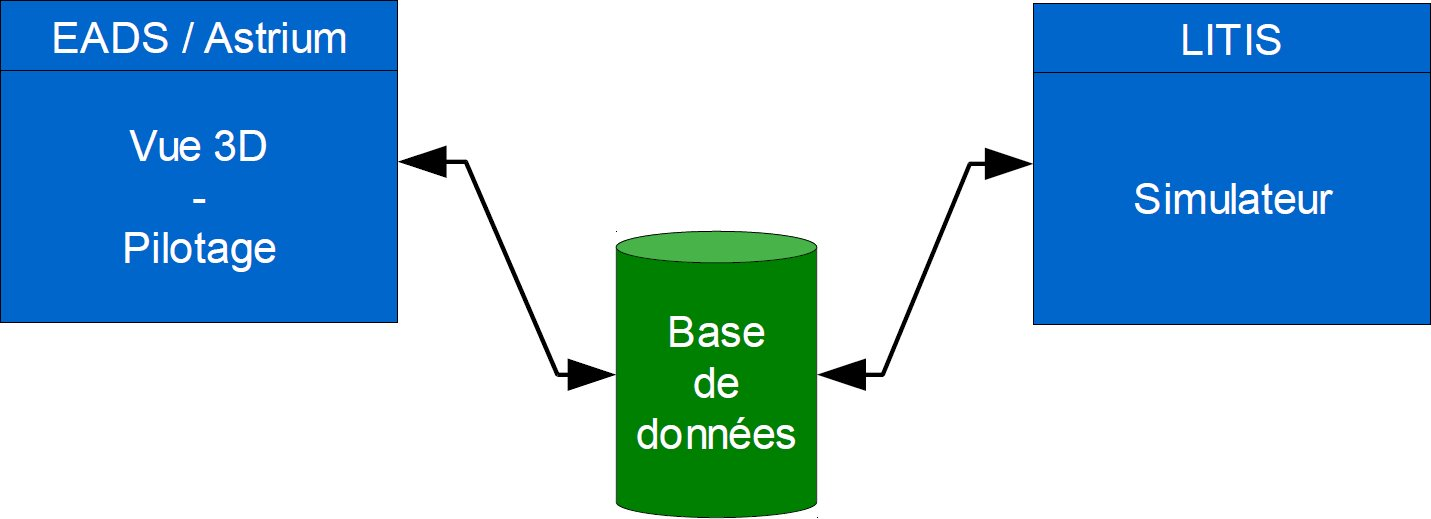
\includegraphics[width=0.75\textwidth]{chapitres/simulation/comEADSLITIS.jpg}
\caption{Communications entre la vue 3D et le simulateur}
\label{fig:simulation:comEADSLITIS}
\end{figure}

La lecture et l'écriture de données dans la base est réalisée à travers des scripts PHP hébergés sur un serveur web ayant accès à la base puis formate le résultat dans un tableau à l'intérieur d'un fichier \verb!XML!. La figure \ref{fig:simulation:scriptPHP} donne un exemple d'accès en lecture à la base de données.

\begin{figure}[ht]
\begin{lstlisting}[language=PHP,escapeinside={@}{@}]
<?php
  try {
    @\$@host = @\$@_POST['host'];
    @\$@dbName = @\$@_POST['dbName'];
    @\$@user = @\$@_POST['user'];
    @\$@password = @\$@_POST['password'];

    @\$@request = @\$@_POST['request'];
    @\$@request = stripslashes(@\$@request);
    @\$@pdo_options[PDO::ATTR_ERRMODE] = PDO::ERRMODE_EXCEPTION;
    @\$@bdd = new PDO("mysql:host=@\$host@;dbname=@\$dbName@", @\$@user, @\$@password, @\$@pdo_options);
    @\$@reponse = @\$@bdd->query(@\$@request);
?>
<table>
<?php while (@\$@donnees = @\$@reponse->fetch()){ ?>
  <tr>
  <?php
    @\$@i=0;
    while(@\$@i < count(@\$@donnees)-1) {
  ?>
    <td>
      <?php echo @\$@donnees[@\$@i]; @\$@i=@\$@i+1; ?>
    </td>
    <?php } ?>
  </tr>
  <?php } ?>
</table>
<?php
  @\$@reponse->closeCursor();
  }
  catch(Exception @\$@e) {
    die('Erreur : '.@\$@e->getMessage());
  }
?>
\end{lstlisting}
\caption{script PHP réalisant une requête sur la base de données}
\label{fig:simulation:scriptPHP}
\end{figure}

\FloatBarrier


\section{Modules proposés}

Le simulateur développé propose une liste extensible de modules.

\subsection{Module de mobilité des chariots cavaliers}

Les chariots peuvent être soit pilotés par une IA, soit par un pilote grâce à un joystick au travers de l'interface 3D de EADS / Astrium. Concernant la partie manuelle, les actions effectuées par le pilote sont inscrites dans la base de données et sont ensuite lues par le simulateur qui reproduit les actions sur le modèle. Aucune vérification d'applicabilité n'est alors effectué puisque cette action est réalisée dans le programme d'EADS / Astrium.
L'IA développée dans le module automatique permet de reproduire le comportement du véhicule en terme de déplacements et d'opérations. Les déplacements consistent à respecter le réseau routier et les zones de stockage du terminal ainsi que d'éviter les collisions entre les véhicules. À chaque itération du simulateur, un véhicule contrôlé par l'IA calcule sa future position en fonction de sa position courante, de sa destination et de sa vitesse. La direction à prendre lui est donnée par le module de routage.

\subsection{Module de routage des véhicules}

Ce module permet de calculer des plus court chemins entre deux points du terminal. Plusieurs algorithmes sont ainsi implémentés et des interfaces sont proposées afin de permettre d'ajouter facilement d'autres algorithmes.

\subsubsection{Floyd Warshall : All Pair Shortest Path}

Cet algorithme calcule une seule fois tous les plus court chemins et sauvegarde les résultats pour que leur récupération soit rapide. La complexité est en $O(n^ 3)$ et le temps d'exécution peut donc être assez long.
Cet algorithme est donc inutilisable dans des graphes trop dynamiques.

\subsubsection{Dijkstra}

Cet algorithme calcule les plus court chemins entre un sommet et tous les autres sommets du graphe. Avec un graphe de m arcs et n n\oe{}uds la complexité est de $O[(m+n)*ln(n)]$.

\subsubsection{A * (A Star)}

Il calcule un plus court chemin entre deux sommets du graphe grâce à une heuristique. C'est un algorithme très rapide mais la qualité de la solution ainsi que sa vitesse d'obtention dépend de l'adaptation de l'heuristique à la topologie du graphe. La complexité de cet algorithme dépend également de l'heuristique utilisée. 
Une seule heuristique a été pour le moment implémentée et réalise une estimation du temps de parcours entre deux sommets en calculant le ratio entre la distance (heuristique de Manhattan) et la vitesse du chariot.

\subsubsection{Dijkstra avec prise en compte des temps d'attente en entrée de travée}

Cet algorithme calcule les plus court chemins en temps entre un sommet et tous les autres sommets du graphe avec prise en compte des blocages dans les travées (arcs FIFO) (voir \ref{chap:contexte:opt:routageVehicules} p\pageref{chap:contexte:opt:routageVehicules}) grâce à un mécanisme de réservation de chemins. La complexité de cet algorithme est semblable à celle de Dijkstra.

\subsection{Module d'ordonnancement des missions}

Ce module permet de calculer l'ordonnancement des missions à réaliser sur le terminal. Les missions sont placées dans un pool de tâches à exécuter par les chariots cavaliers. Ces derniers représentent donc des ressources. Le calcul doit tenir compte des fenêtres de temps des missions afin de proposer une solution acceptable pour les clients du terminal (navires, trains ou camions).

\begin{figure}[h]
\centering
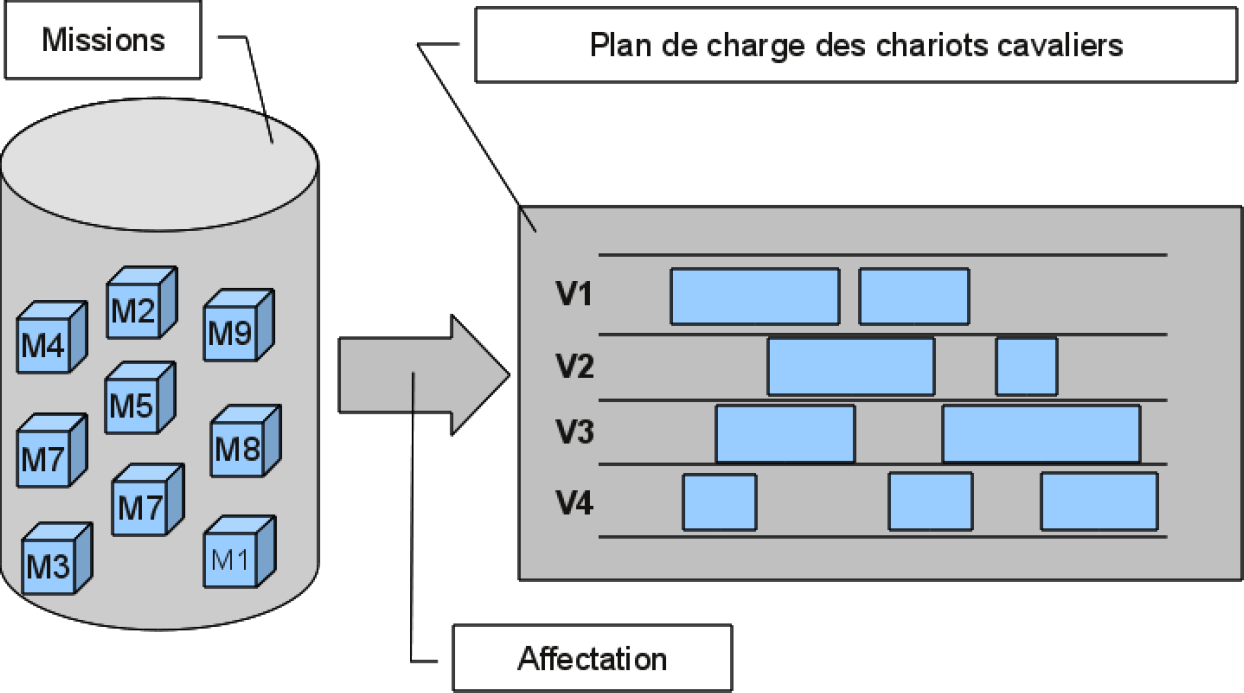
\includegraphics[width=0.75\textwidth]{chapitres/simulation/ordonnancement.png}
\caption{Affectation des missions aux chariots cavaliers}
 \label{fig:simulation:ordonnancement}
\end{figure}

Dans le soucis de réduire les coûts d'exploitation du terminal ainsi que de maintenir une qualité de service suffisante pour les clients, le système doit prendre en compte plusieurs paramètres lors de l'affectation des missions de chargement/déchargement aux chariots cavaliers. Ainsi, la distance à effectuer et le temps de parcours lié à une mission va avoir un impact direct sur le coût de la mission pour le chariot cavalier (consommation de carburant, temps occupé) ainsi que sur le respect des fenêtres de temps pour le client. En effet, si le chariot cavalier arrive trop tard sur le lieu de collecte ou de livraison, le client devra l'attendre. Cette attente a un coût et le client peut réclamer des indemnités au terminal. En revanche, si le chariot cavalier arrive en avance sur le lieu de collecte/livraison, alors il devra attendre le client devenant ainsi indisponible pour d'autres tâches dans le même temps. Plusieurs algorithmes sont développés afin de répondre à ces problématiques. Ils peuvent être statiques ou dynamiques. Les algorithmes statiques sont performants mais demandent de recalculer entièrement une solution dès qu'une mission est insérée ou supprimée ou qu'une ressource devient indisponible. En revanche, les algorithmes dynamiques proposent des solutions ``acceptables'' à tout moment.

Chaque algorithme d'ordonnancement et d'affectation présenté dans le chapitre \ref{chapitre:ordo} a été implémenté dans le simulateur. Le module d'ordonnancement contient donc les algorithmes décris dans le tableau suivant : 

% \begin{center}
%  \footnotesize
% \begin{tabular}{|p{7.9cm} p{2.75cm}| p{3.8cm}|}
% 
%   \hline 
%  \multicolumn{2}{|c|}{\textbf{Algorithme}} & \multicolumn{1}{c|}{\textbf{rmiBindingName}} \tabularnewline \hline
%  Branch-and-Bound & (voir \ref{chap:ordo:reso:BB} p\pageref{chap:ordo:reso:BB}) & BranchAndBoundScheduler \tabularnewline \hline
%  Aléatoire & (voir \ref{chap:ordo:reso:random} p\pageref{chap:ordo:reso:random}) & RandomScheduler \tabularnewline \hline
%  Répartition de charge & (voir \ref{chap:ordo:reso:linear} p\pageref{chap:ordo:reso:linear}) & LinearScheduler \tabularnewline \hline
%  Gloutonne : heuristique des plus proches voisins & (voir \ref{chap:ordo:sec:resolution:subsec:heuristiques:glouton} p\pageref{chap:ordo:sec:resolution:subsec:heuristiques:glouton}) & GreedyScheduler \tabularnewline \hline
%  Gloutonne élaborée & (voir \ref{chap:ordo:reso:greedyOpt} p\pageref{chap:ordo:reso:greedyOpt}) & GreedyOptScheduler \tabularnewline \hline
%  Métaheuristique fourmi hors-ligne & (voir \ref{chap:ordo:reso:offlineACO} p\pageref{chap:ordo:reso:offlineACO}) & OfflineACOScheduler \tabularnewline \hline
%  Métaheuristique fourmi en-ligne & (voir \ref{chap:ordo:reso:onlineACO} p\pageref{chap:ordo:reso:onlineACO}) & OnlineACOScheduler \tabularnewline \hline
% \end{tabular}
% \end{center}

\begin{center}
 \footnotesize
\begin{tabular}{|p{10cm}| p{3.8cm}|}
 \hline 
 \multicolumn{1}{|c|}{\textbf{Algorithme}} & \multicolumn{1}{c|}{\textbf{rmiBindingName}} \tabularnewline \hline
 Branch-and-Bound (voir \ref{chap:ordo:reso:BB} p\pageref{chap:ordo:reso:BB}) & BranchAndBoundScheduler \tabularnewline \hline
 Aléatoire (voir \ref{chap:ordo:reso:random} p\pageref{chap:ordo:reso:random}) & RandomScheduler \tabularnewline \hline
 Répartition de charge (voir \ref{chap:ordo:reso:linear} p\pageref{chap:ordo:reso:linear}) & LinearScheduler \tabularnewline \hline
 Gloutonne : heuristique des plus proches voisins (voir \ref{chap:ordo:sec:resolution:subsec:heuristiques:glouton} p\pageref{chap:ordo:sec:resolution:subsec:heuristiques:glouton}) & GreedyScheduler \tabularnewline \hline
 Gloutonne élaborée (voir \ref{chap:ordo:reso:greedyOpt} p\pageref{chap:ordo:reso:greedyOpt}) & GreedyOptScheduler \tabularnewline \hline
 Métaheuristique fourmi hors-ligne (voir \ref{chap:ordo:reso:offlineACO} p\pageref{chap:ordo:reso:offlineACO}) & OfflineACOScheduler \tabularnewline \hline
 Métaheuristique fourmi en-ligne (voir \ref{chap:ordo:reso:onlineACO} p\pageref{chap:ordo:reso:onlineACO}) & OnlineACOScheduler \tabularnewline \hline
\end{tabular}
\end{center}

\subsection{Module de représentation 2D du terminal}

Ce module permet de visualiser en 2 dimensions l'évolution du terminal. Il contient trois parties :
\begin{itemize}
 \item la vue;
 \item la partie informative;
 \item la partie contrôle;
 \item la partie ordonnancement.
\end{itemize}

\subsubsection{Vue}

La partie vue représente le graphe routier du terminal, le réseau de stockage, les conteneurs et les chariots cavaliers. Cette vue utilise la librairie GraphStream (voir \href{http://graphstream-project.org}{http://graphstream-project.org}) permettant de dessiner entièrement ces éléments de façon très simple grâce à des feuilles de style \verb!CSS!. Le module développé propose un \verb!Listener! sur les modifications du terminal et permet à l'utilisateur de définir des actions en cas d'ajout/suppression de routes ou de conteneurs, de déplacement de véhicule, etc. De cette façon, à tout moment, la vue 2D représente graphiquement et avec exactitude l'état du système.

\subsubsection{Informations}

La partie informative du module de représentation 2D contient des informations sous forme de texte à propos de l'état du terminal. On y trouve des informations sur les missions connues du systèmes (conteneur concerné, destination, fenêtres de temps, état, chariot cavalier affecté...), sur les conteneurs (position), sur les véhicules (position, état, plan de charge) ou sur les travées du terminal (contenu des emplacements). Lorsqu'un élément est sélectionné par l'utilisateur dans cette vue, les éléments de la vue 2D concernés par ces informations sont mis en évidence graphiquement. Cette vue est développée en \verb!JAVA! au travers de la librairie \verb!Swing!.

\subsubsection{Contrôleur}

La partie contrôle concerne le déroulement de la simulation. Elle permet à l'utilisateur de définir le pas de temps, puis de démarrer la simulation. Une fois lancée, il peut également la mettre en pause et avancer itération par itération, relancer la simulation ou quitter le programme. D'autre part, dans le cas où un chariot se trouve dans l'impossibilité de prendre/déposer un conteneur (conteneur bloqué sous un autre, problème d'alignement, problème d'étage, emplacement plein, etc), une boîte de dialogue apparaît et demande à l'utilisateur de régler ce problème. Pour cela, la boîte de dialogue propose des solutions et l'utilisateur n'a plus qu'à faire son choix.

\begin{figure}[h]
\centering
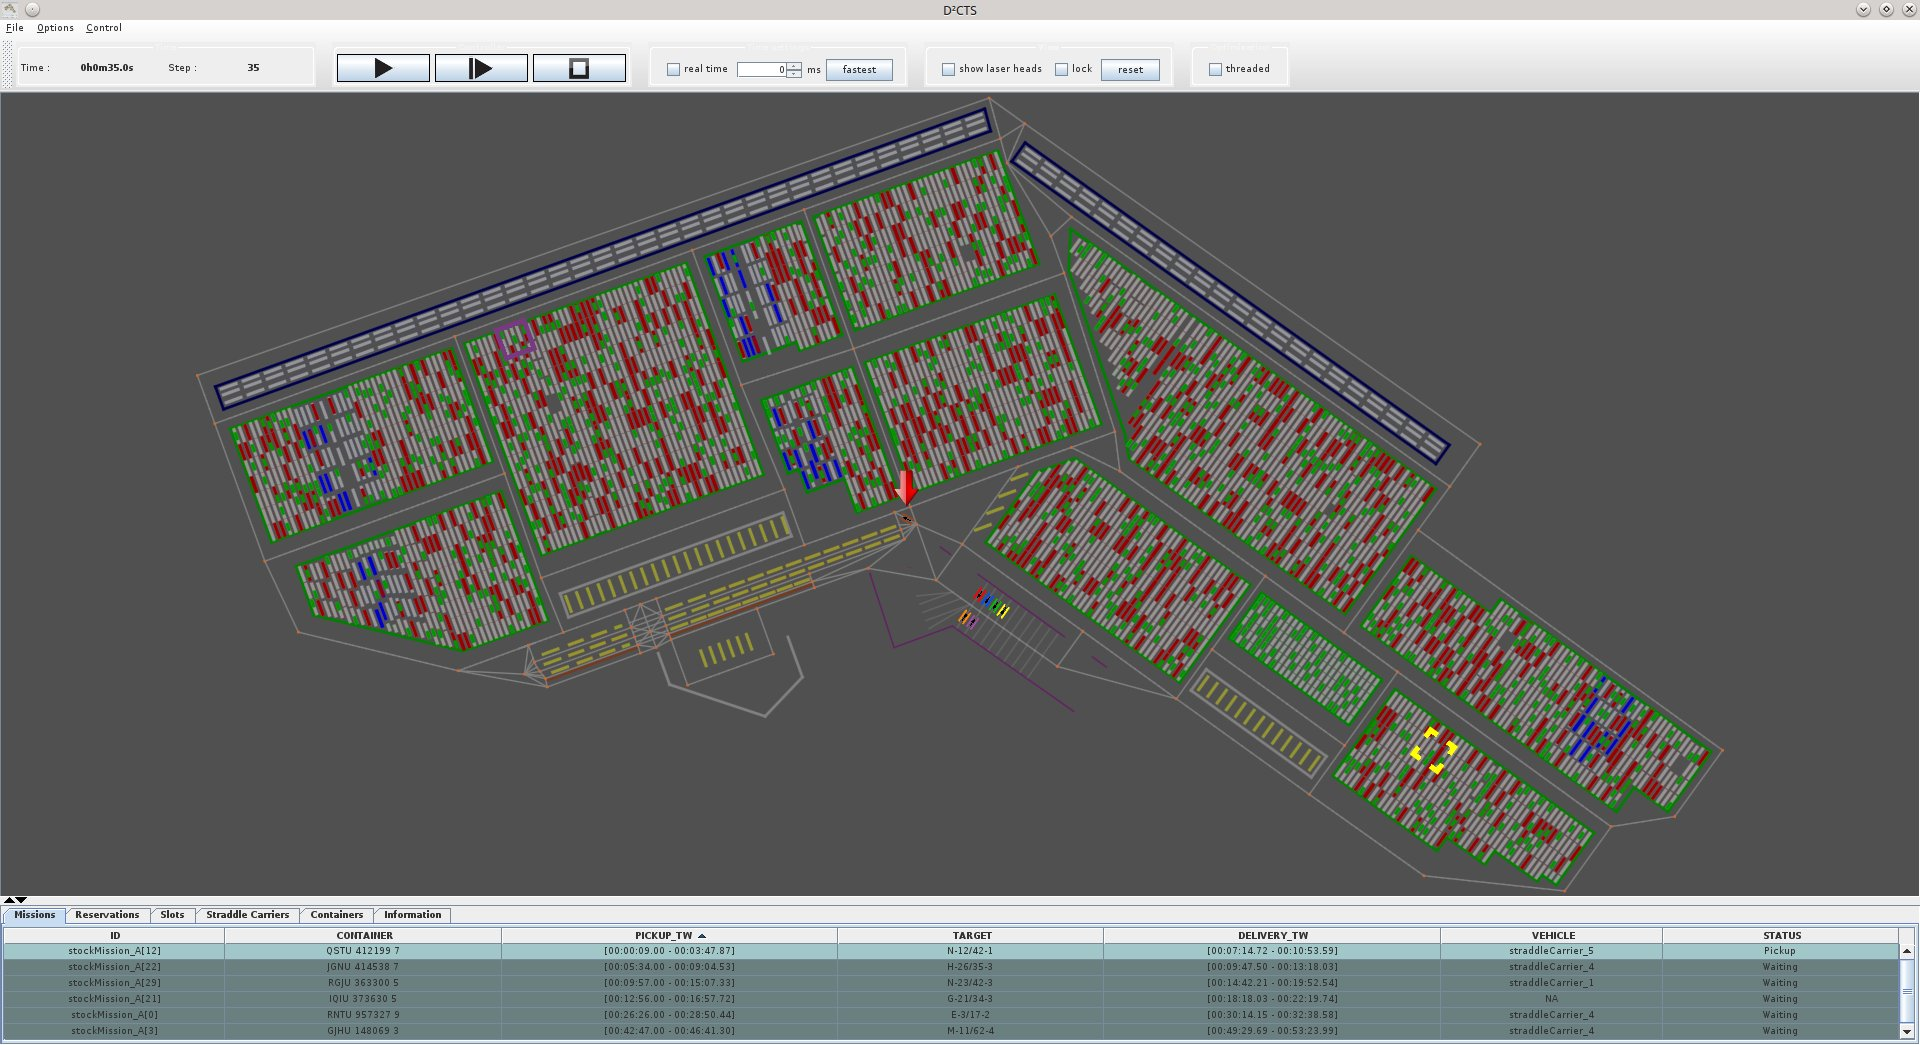
\includegraphics[width=0.85\textwidth]{chapitres/simulation/vue2D-vue-controle-infos.jpg}
\caption{Capture de la partie principale du module graphique du simulateur (en haut le contrôleur, au centre la vue du terminal, en bas la partie informative)}
 \label{fig:simulation:ihm2D}
\end{figure}

\subsubsection{Ordonnanceur}

La partie ordonnancement concerne la performance des affectations des missions aux chariots cavaliers. Selon les critères établis dans le chapitre précédent, cette performance dépend de la distance couverte par les véhicules, du retard lié au dépassement des fenêtres de temps (\textit{tardiness}), ainsi que de la durée d'attente des véhicules aux points de collecte et de livraison (\textit{earliness}). Lorsque l'algorithme de résolution le défini, des données supplémentaires peuvent être affichées, comme le graphe de résolution par exemple pour la méthode de résolution en-ligne utilisant la métaheuristique fourmi.

\begin{figure}[h]
 \centering
 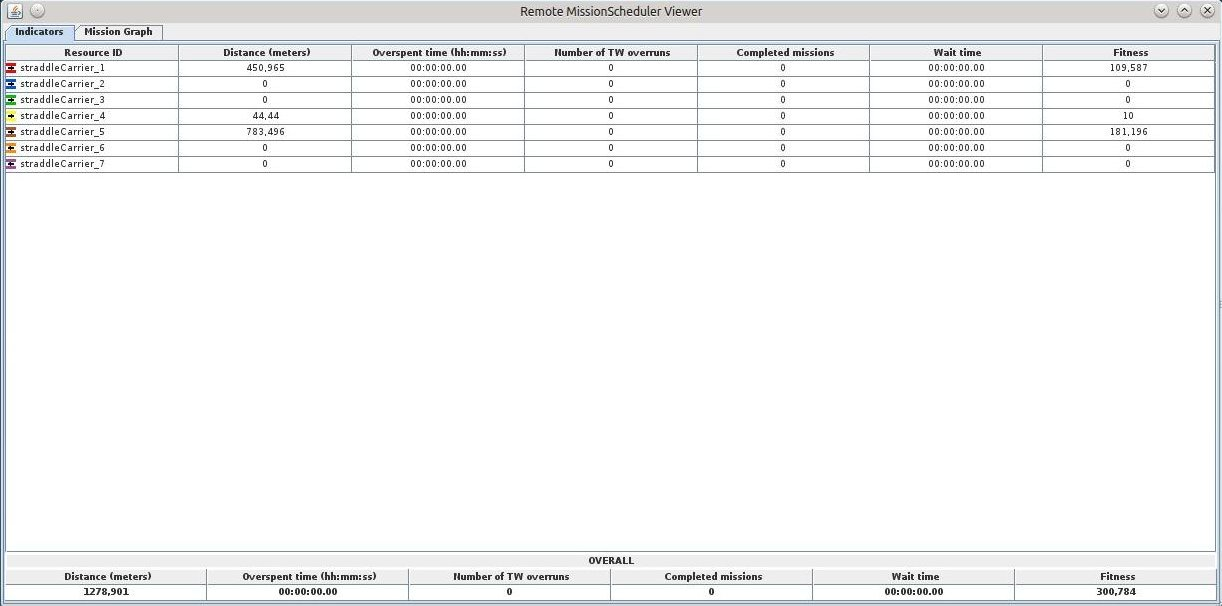
\includegraphics[width=0.85\textwidth]{chapitres/simulation/ordo2D-Infos.jpg}
 \caption{Partie ordonnancement du module graphique du simulateur : informations sur la performance de l'algorithme}
 \label{fig:simulation:ordonnancement2D}
\end{figure}

\begin{figure}[h]
 \centering
 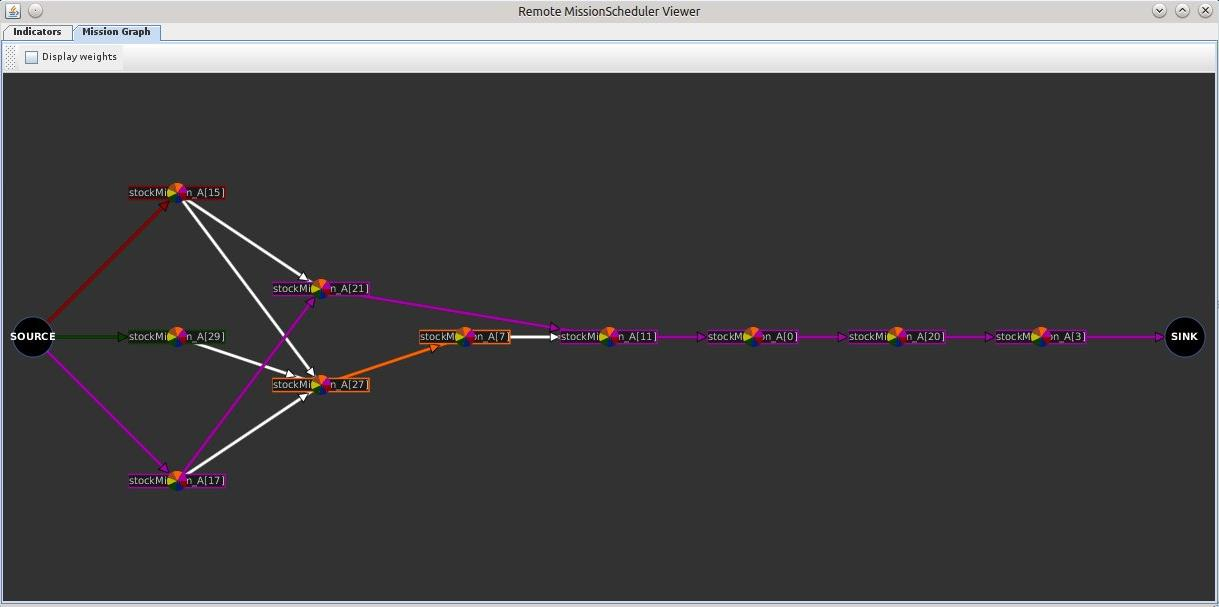
\includegraphics[width=0.85\textwidth]{chapitres/simulation/ordo3D-Graphe.jpg}
 \caption{Partie ordonnancement du module graphique du simulateur : graphe des missions de l'algorithme de résolution en-ligne}
 \label{fig:simulation:ordonnancement2D-2}
\end{figure}

\subsection{Module de transformation XML (\textit{parser})}

Ce module permet de transformer les données \verb!XML! concernant la simulation en informations. Il se compose de 3 parties :
\begin{itemize}
 \item Le \textit{parser} de configuration réseau : transforme les informations décrites dans le fichier de distribution (voir \ref{chap:simulateur:sec:archi:distribution:reseau} p\pageref{chap:simulateur:sec:archi:distribution:reseau});
 \item Le \textit{parser} de configuration du terminal : transforme selon le format défini (voir \ref{chap:simulateur:sec:archi:distribution:contenu} p\pageref{chap:simulateur:sec:archi:distribution:contenu}) les éléments \verb!XML! en objets informatiques afin de décrire les composants du terminal ainsi que son contenu;
 \item Le \textit{parser} de communication avec les chariots cavaliers : permet de définir les actions à réaliser par l'IA des chariots cavaliers en fonctions de messages \verb!XML!.
\end{itemize}
C'est dans ce module que sont définies les règles d'écritures des balises. Un modèle différent peut donc être facilement implémenté en redéfinissant ces classes.

\subsection{Modules de génération de données}
Les générateurs proposés sont des modules permettant de générer des fichiers \verb!XML!. Il existe pour le moment 3 générateurs de données :
\begin{itemize}
 \item le générateur d'état initial;
 \item le générateur de missions;
 \item le générateur d'événements.
\end{itemize}

\subsubsection{Générateur d'état initial}

Ce générateur permet de créer des conteneurs et de les répartir entre les différents emplacements de stockage du terminal. Il utilise les fichiers de configuration du terminal afin de définir la structure du terminal et de connaître son contenu. Il charge donc le graphe routier et le réseau de stockage avant de commencer à générer les conteneurs. La génération se fait selon différents paramètres. Il faut en effet fournir au générateur le nombre de conteneurs de 20 pieds, de 40 pieds et de 45 pieds à créer. De plus, il faut indiquer le nom de la machine sur laquelle le générateur est lancé ainsi que les fichiers de configuration réseau et de terminal à utiliser. Enfin il faut définir le nom du fichier \verb!XML! à générer.

\subsubsection{Générateur de missions}

Ce générateur permet de créer des missions pour les chariots cavaliers. Une mission consiste à déplacer un conteneur à l'intérieur du terminal. Selon le type de mission à définir, le générateur va créer ou non un véhicule (train, bateau, ou navire). Il détermine également si la mission à créer sera de type \verb!IN! ou \verb!OUT! puis, en fonction du résultat décidera du conteneur à déplacer. Si le conteneur entre dans le terminal (mission de type \verb!IN!) alors il sera créé. Ensuite le générateur défini un emplacement de destination pour la livraison du conteneur. Une fois ces informations déterminées le générateur détermine les fenêtres de temps de la mission ainsi que les fenêtres de temps des véhicules concernés. Pour cela il se base sur le temps moyen de parcours entre le point de collecte et de livraison du conteneur. Les fenêtres de temps sont ensuite décalées selon une marge de tolérance d'écart de temps. Ce paramètre est fourni en entrée de l'algorithme.

\subsubsection{Générateurs d'événements}

Le générateur d'événements permet de générer un fichier \verb!XML! contenant des balises \verb!<event>!\verb!</event>! afin de décrire des perturbations sur le système. Il est possible de générer des pannes sur les véhicules, des non respect d'itinéraires par les conducteurs ou de non respect d'affectation de mission. Il est également possible de générer des variations de portée des bornes lasers. Ces événements sont définis en fonction de taux indiqués en entrée du générateur.


L'objectif final de ces générateurs est de pouvoir les configurer en fonction de lois statistiques. Ainsi, les modules de générations sont composés d'interfaces permettant aux utilisateurs de redéfinir les fonctions de générations selon les besoins.

\section{Perspectives}

Les deux premières années de travail sur le projet CALAS ont consisté à modéliser les composants d'un terminal portuaire ainsi que leur dynamique. Le simulateur informatique de terminal a été élaboré autour de l'informatisation du plan du terminal de Normandie grâce à une longue phase de collecte de données.

Le simulateur développé a été conçu pour mettre à l'épreuve différentes approches d'ordonnancement et de routage pour obtenir des résultats permettant d'évaluer la qualité des diverses solutions. Toutefois, il est possible d'utiliser le simulateur pour concevoir des méthodes de résolution à tous les problèmes d'optimisation liés aux terminaux à conteneurs. Il est ainsi possible de mettre à l'épreuve des approches de résolution des problèmes de : 
\begin{itemize}
 \item la structure du terminal;
 \item l’allocation des berges aux navires;
 \item l’allocation des grues de quai;
 \item les plans de chargement des navires;
 \item le transbordement;
 \item la gestion des conteneurs vides;
 \item la gestion des effectifs;
 \item le stockage (allocation des travées et des blocs) ;
 \item les transferts (quai - stockage, stockage - stockage, stockage - terre);
 \item le routage des véhicules;
 \item l’allocation des engins de manutention.
\end{itemize}

Pour le moment, le simulateur n'a été utilisé que pour modéliser les 2 derniers problèmes, néanmoins il est capable de façon intrinsèque de répondre aux autres problématiques.


	%%%%%%%%%%
	\section*{Conclusions}\label{partie:simulation-conclusions}
	\addcontentsline{toc}{section}{Conclusions}
	%Conclusion sur l'application

Un terminal multimodal à conteneurs est une plate-forme logistique d'échange de marchandises ouverte à la fois sur la terre et sur l'eau. Leur développement important montre l'importance des enjeux économiques de ces structures qui doivent être de plus en plus performantes en terme de rapidité de service et de coûts d'exploitation.
L'optimisation du terminal est donc essentielle et concerne différents problèmes comme la définition de la structure du terminal, de l'allocation des berges, des portiques de quai, du positionnement des conteneurs, du routage des véhicules ainsi que de l'affectation des opérations de déplacement de conteneurs.\\


Ce chapitre à permis de définir les tenants et les aboutissants du contexte applicatif de cette thèse et à introduit le problème d'ordonnancement et d'affectation des missions aux chariots cavaliers qui sera étudié dans le chapitre suivant.

	%%%%%%%%%%%%%%%%%%%%%%%%%%%%%%%%%%%%%%%%%%%%%%%%%%%%%%%
	%%%%%%%%            RESULTATS		 	%%%%%%%
	%%%%%%%%%%%%%%%%%%%%%%%%%%%%%%%%%%%%%%%%%%%%%%%%%%%%%%%  
	\chapter{Expérimentations et résultats}\label{chapitre:resultats}

	\section*{Introduction}\label{partie:resultats-introduction}
	\addcontentsline{toc}{section}{Introduction}
	%Introduction chapitre III : Simulation

Ce chapitre présente $D^2CTS$ : un simulateur de terminal portuaire à conteneurs conçu et développé durant cette thèse. Les problèmes d'ordonnancement et d'affectation ainsi que de routage dynamique sont des problématiques théoriques ici inscrites dans un contexte concret. Les terminaux portuaires à conteneurs sont des structures privées difficilement abordables. Ils fonctionnent en continu et il est donc impossible de procéder à des tests grandeur nature sur une journée d'exploitation. Un simulateur permet ainsi de réaliser ces mesures de performance dans un environnement virtuel le plus réaliste possible avant d'hypothétiquement passer à la mise en place à l'échelle réelle. 

Le programme a été élaboré lors de la participation du LITIS au projet CALAS qui est l'acronyme de \textit{CArrier LAser tracking System}. Le projet consiste à élaborer une technologie de localisation des engins de manutention capable de fonctionner à n'importe quel endroit du terminal. En effet, la technologie de géolocalisation actuelle utilise des satellites (GPS : \textit{Global Positioning System}%TODO CHECK
) afin de déterminer les coordonnées d'un émetteur. Or, le signal des satellites traversant mal le métal, les véhicules qui se trouvent sous les portiques de déchargement ou dans les travées de conteneurs ne sont pas repérés.

La société \textit{Laser Data Technology Terminal} (LDTT) a mis au point une technologie de géolocalisation utilisant un rayon laser et exploitant la caractéristique physique principale des chariots cavaliers : leur hauteur. En effet, les chariots cavaliers sont les engins mobiles autonomes les plus élevés du terminal. Il est donc possible de déterminer leur position grâce à un signal horizontal émis à la hauteur du sommet des chariots cavaliers afin d'être en mesure de localiser les véhicules équipés à n'importe quel endroit du terminal. Le système est composé d'un réseau d'émetteurs/récepteurs laser (\textit{InfraRed Intelligent Sensors}) IRIS répartis sur le terminal (voir figure \ref{fig:bornesLaser}). D'autres bornes IRIS sont installées sur les chariots cavaliers et permettent de réaliser une triangularisation du signal infrarouge (voir figure \ref{fig:triangularisation}).


\begin{figure}[ht]
\centering
 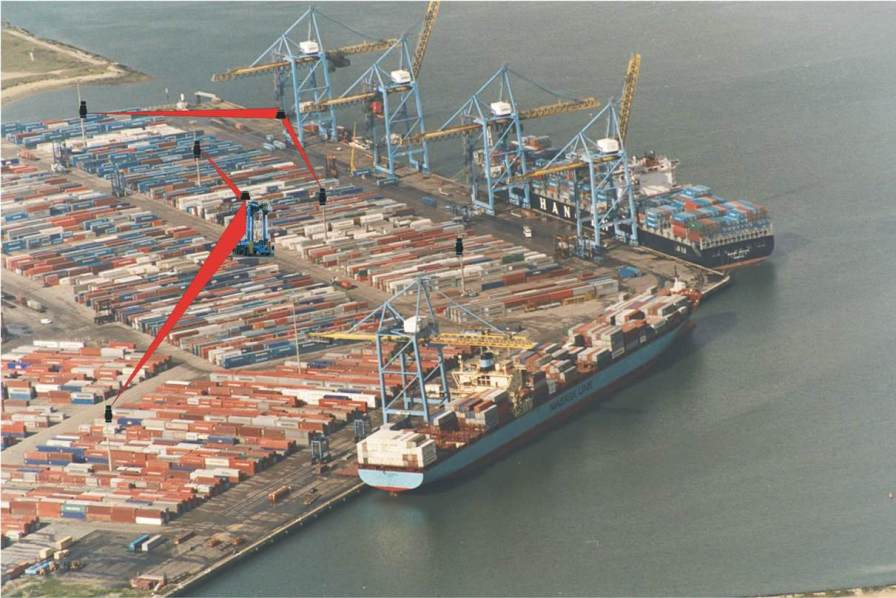
\includegraphics[width=0.6\textwidth]{./chapitres/simulation/bornesLaser.jpg}
  \caption{Réseau de bornes laser implantées sur le Terminal de Normandie (source : \href{http://www.ldtt-fr.com}{http://www.ldtt-fr.com})}
  \label{fig:bornesLaser}
\end{figure}

\begin{figure}[ht]
\centering
 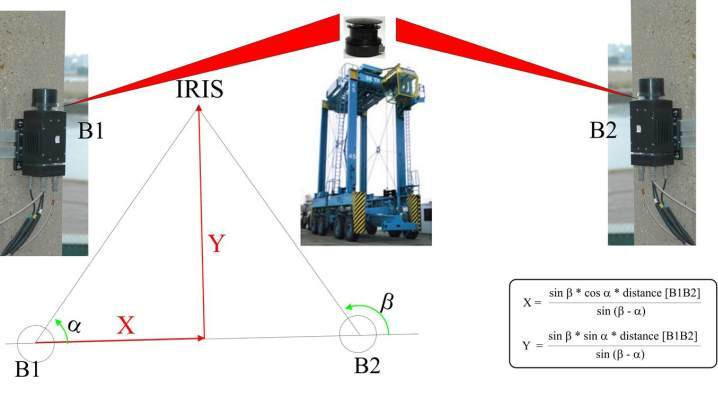
\includegraphics[width=0.6\textwidth]{./chapitres/simulation/triangularisationLaser.jpg}
  \caption{Triangularisation du signal infrarouge entre les bornes IRIS du terminal et celle d'un chariot cavalier (source : \href{http://www.ldtt-fr.com}{http://www.ldtt-fr.com})}
  \label{fig:triangularisation}
\end{figure}

Après plusieurs années de développement et de tests réels, cette technologie se montre performante et fiable et permet de connaître en temps réel la position des engins de manutention au sein du terminal. Cette information est la condition \textit{sine qua non} à toute recherche d'optimisation dynamique des activités des engins de manutention. Grâce à la position des véhicules il est ainsi possible d'optimiser dynamiquement le routage des chariots cavaliers et de prendre en compte les durées de parcours au sein du terminal. Ceci permet par conséquent, d'optimiser l'activité des chariots cavaliers tout en contrôlant le suivi de leurs opérations. En effet, lorsqu'un conteneur est chargé ou déposé par un chariot cavalier, un signal contenant la position du véhicule est envoyé au système. Ainsi, le système connaît la position de prise du conteneur (et par conséquent le conteneur chargé) ainsi que sa position de dépose. Ces informations permettent d'éviter les pertes de conteneurs au sein du terminal.

La partie LITIS du projet consistait à proposer des méthodes d'optimisation dynamique des activités des chariots cavaliers en utilisant l'information fournie par le système de géolocalisation laser. 


	%%%%%%%%%%
% 	\section{Routage des chariots cavaliers}\label{partie:resultats-routage}
 	\section{Protocole de test}\label{partie:resultats-protocole}
	 
	

	%%%%%%%%%%
	\section{Résultats}\label{partie:resultats-ordonnancement}
	 

	
	%%%%%%%%%%
	\section{Analyse et discussion}\label{partie:analyse-discussion}
	 


	%%%%%%%%%%
	\section*{Conclusions}\label{partie:resultats-conclusions}
	\addcontentsline{toc}{section}{Conclusions}
	%Conclusion sur l'application

Un terminal multimodal à conteneurs est une plate-forme logistique d'échange de marchandises ouverte à la fois sur la terre et sur l'eau. Leur développement important montre l'importance des enjeux économiques de ces structures qui doivent être de plus en plus performantes en terme de rapidité de service et de coûts d'exploitation.
L'optimisation du terminal est donc essentielle et concerne différents problèmes comme la définition de la structure du terminal, de l'allocation des berges, des portiques de quai, du positionnement des conteneurs, du routage des véhicules ainsi que de l'affectation des opérations de déplacement de conteneurs.\\


Ce chapitre à permis de définir les tenants et les aboutissants du contexte applicatif de cette thèse et à introduit le problème d'ordonnancement et d'affectation des missions aux chariots cavaliers qui sera étudié dans le chapitre suivant.
	
	%%%%%%%%%%%%%%%%%%%%%%%%%%%%%%%%%%%%%%%%%%%%%%%%%%%%%%%
	%%%%%%%%         	 CONCLUSIONS		%%%%%%%
	%%%%%%%%%%%%%%%%%%%%%%%%%%%%%%%%%%%%%%%%%%%%%%%%%%%%%%%  
	\chapter*{Conclusions}\label{chapitre:conclusions}
	\addcontentsline{toc}{chapter}{Conclusions}
	%Conclusion sur l'application

Un terminal multimodal à conteneurs est une plate-forme logistique d'échange de marchandises ouverte à la fois sur la terre et sur l'eau. Leur développement important montre l'importance des enjeux économiques de ces structures qui doivent être de plus en plus performantes en terme de rapidité de service et de coûts d'exploitation.
L'optimisation du terminal est donc essentielle et concerne différents problèmes comme la définition de la structure du terminal, de l'allocation des berges, des portiques de quai, du positionnement des conteneurs, du routage des véhicules ainsi que de l'affectation des opérations de déplacement de conteneurs.\\


Ce chapitre à permis de définir les tenants et les aboutissants du contexte applicatif de cette thèse et à introduit le problème d'ordonnancement et d'affectation des missions aux chariots cavaliers qui sera étudié dans le chapitre suivant.	
	
	
      % BIBLIOGRAPHIE
      \bibliographystyle{apalike}
      \bibliography{bibliographie/bibliographie_these}  % include bibliography
      
      % INDEX ?
      %\include{index}
\end{document}
